% !TEX program = xelatex
% ============================================================
% 北京高校数学建模校际联赛 / 数学建模竞赛论文 LaTeX 模板
% 编译方式：XeLaTeX（Overleaf 中选择 XeLaTeX）
% 说明：
% 1. 本模板默认 A4 纸，四周页边距 2.5 cm。
% 2. 默认无页眉，页码位于页脚居中，从摘要页开始编号为 1。
% 3. 第一页仅放论文标题、摘要、关键词；正文从第二页开始。
% 4. 不含学校、姓名、队员编号等身份信息，请勿在正文、附录、文件名、代码路径中出现身份信息。
% 5. 正文默认宋体五号字；一级标题黑体四号，二、三级标题黑体五号。
% ============================================================

\documentclass[UTF8,a4paper,zihao=5,fontset=fandol]{ctexart}

% ---------- 页面与字体 ----------
% 正文：宋体五号。ctex 会根据编译环境自动调用可用宋体/等价宋体；
% 在 Overleaf 或本地 TeXLive 中通常会使用 FandolSong，Windows 中通常对应 SimSun。
\AtBeginDocument{\songti\zihao{5}}
\usepackage{geometry}
\geometry{top=2.5cm,bottom=2.5cm,left=2.5cm,right=2.5cm}
\usepackage{setspace}
\setstretch{1.25}
\setlength{\parindent}{2em}
\setlength{\parskip}{0pt}

% ---------- 数学、图表、列表 ----------
\usepackage{amsmath,amssymb,amsfonts,bm,mathtools}
\usepackage{graphicx}
\usepackage{float}
\usepackage{subcaption}
\usepackage{booktabs,longtable,tabularx,array,multirow,makecell}
\usepackage{enumitem}
\usepackage{xcolor}
\usepackage{caption}
\usepackage{listings}
\usepackage{hyperref}
\newCJKfontfamily{\songtifallback}{Songti SC}

% ---------- 页眉页脚：不设页眉，仅页脚中部页码 ----------
\pagestyle{plain}
\pagenumbering{arabic}
\setcounter{page}{1}

% ---------- 章节格式 ----------
\ctexset{
  section = {
    name = {,、},
    number = \chinese{section},
    format = \zihao{4}\heiti\raggedright,
    aftername = \hspace{0.25em},
    beforeskip = 1.0em,
    afterskip = 0.55em
  },
  subsection = {
    format = \zihao{5}\heiti\raggedright,
    aftername = \hspace{0.35em},
    beforeskip = 0.75em,
    afterskip = 0.35em
  },
  subsubsection = {
    format = \zihao{5}\heiti\raggedright,
    aftername = \hspace{0.35em},
    beforeskip = 0.5em,
    afterskip = 0.25em
  }
}

% ---------- 图表标题 ----------
\captionsetup{font=normalsize,labelsep=space}
\numberwithin{equation}{section}
\numberwithin{figure}{section}
\numberwithin{table}{section}
\allowdisplaybreaks[4]

% ---------- 超链接 ----------
\hypersetup{
  colorlinks=true,
  linkcolor=black,
  citecolor=black,
  urlcolor=black,
  pdfauthor={},
  pdftitle={数学建模竞赛论文}
}

% ---------- 列表样式 ----------
\setlist[itemize]{leftmargin=2.2em,itemsep=0.15em,topsep=0.2em}
\setlist[enumerate]{leftmargin=2.6em,itemsep=0.15em,topsep=0.2em}

% ---------- 代码样式：若代码中包含大量中文注释，建议改用支撑文件提交，不强行全文排入正文 ----------
\lstset{
  basicstyle=\ttfamily\small,
  numbers=left,
  numberstyle=\tiny,
  frame=single,
  breaklines=true,
  columns=fullflexible,
  keepspaces=true,
  showstringspaces=false,
  tabsize=4,
  keywordstyle=\bfseries,
  xleftmargin=2em,
  framexleftmargin=1.5em
}

% ---------- 常用自定义命令 ----------
\newcommand{\diff}{\mathrm{d}}
\newcommand{\E}{\mathbb{E}}
\newcommand{\Var}{\mathrm{Var}}
\newcommand{\R}{\mathbb{R}}

\begin{document}

% ============================================================
% 第一页：标题、摘要、关键词。摘要不超过一页。
% ============================================================
\thispagestyle{plain}

\begin{center}
  {\zihao{3}\heiti 基于相对运动坐标与相似模板迁移的台风降水时空生成模型}\\[1.2em]
\end{center}

\begin{center}
  {\heiti 摘要}
\end{center}

台风极端降水具有明显的时空非均匀性，其形成和演变不仅受台风路径、强度和移动过程影响，也与海陆分布、近岸过程和地形环境等因素密切相关。本文基于 CMABST 台风路径资料和 GPM 半小时降水资料，围绕“路径--强度--环境--降水”的关系，建立了台风降水结构分析、缺测台风降水场生成和未来虚拟台风情景模拟的综合模型。首先对路径资料与降水资料进行时间对齐和空间匹配，构建降水结构指标体系；随后通过相关性分析和机器学习模型识别影响降水分布的关键因素；最后利用历史相似样本、\textbf{台风相对运动坐标系}、\textbf{EOF/PCA 结构修正}和\textbf{极端分位数校准}方法，生成目标台风及虚拟台风的可能降水时空分布。

针对问题一，本文首先建立以台风中心和移动方向为基准的\textbf{相对运动坐标系}，提取最大降水强度、P95 降水强度、强降水面积、降水质心偏移、前后左右非对称性和雨带各向异性等指标；同时引入最大风速、中心气压、移动速度、移动方向、距岸距离、陆地覆盖比例和地形起伏等解释变量，形成路径、强度、移动和环境共同作用下的降水特征指标体系。在此基础上，本文采用 Spearman 相关性分析和\textbf{增强随机森林模型}，定量分析各类台风因素对降水空间结构的影响。结果表明，模型对降水质心偏移和雨带各向异性的测试集 $R^2$ 分别达到 0.684 和 0.640，说明所构建的路径--强度--环境变量能够较好解释台风降水空间结构变化。

针对问题二，由于 2024 年 KONG-REY 和 MAN-YI 在 GPM 降水数据中没有对应记录，本文将其降水模拟转化为\textbf{条件降水场生成问题}。模型首先从历史台风样本中检索与目标时刻路径、强度、移动和近岸条件相似的时次，再将历史降水模板统一到台风相对运动坐标系中进行\textbf{相似模板迁移与加权融合}，并通过 \textbf{EOF/PCA} 方法修正大尺度空间结构，最后利用\textbf{极端分位数校准}恢复强降水尾部特征。最终生成了两场台风的完整半小时可能降水过程，其中 KONG-REY 和 MAN-YI 分别包含 421 和 553 个半小时时次，最大格点雨强分别为 53.733 mm/hr 和 54.405 mm/hr，主雨区均表现为移动方向左前侧占优。

针对问题三，本文以 KONG-REY 为基准台风，构造强度增强、路径近岸偏移、近岸段偏移、移速减慢和复合扰动等\textbf{虚拟台风情景}，并将扰动后的路径、强度、移动和环境变量重新输入前述条件降水场生成模型，从而得到未来情景下的半小时降水时空分布。结果表明，移速减慢情景对固定地理位置上的累计降水和持续时间放大最为明显：相较基准情景，S4 情景的最大累计降水由 723.48 mm 增至 1208.09 mm，固定地理格点最大强降水持续时间由 24.5 h 增至 39.0 h，说明台风移动速度减慢可能显著增强极端降水的滞留风险。

为检验模型可靠性，本文进一步设计\textbf{历史台风伪缺失实验}，将有真实 GPM 记录的历史台风视为未知降水事件，并用同一生成流程进行反推验证。验证结果显示，极端分位数校准后，P95 误差、P99 误差和 $10\ \mathrm{mm/hr}$ 强降水面积误差分别较初始模板场降低 39.73\%、39.41\% 和 37.13\%，说明本文模型能够较好恢复台风极端降水强度和强降水区域。综合来看，本文模型兼具物理解释性和数据驱动能力，可为台风极端降水风险识别和未来情景评估提供定量参考。

\vspace{0.8em}
\noindent{\heiti 关键词：}\textbf{台风降水}；\textbf{相对运动坐标系}；\textbf{随机森林}；\textbf{相似模板迁移}；\textbf{极端分位数校准}；\textbf{虚拟台风情景}

\newpage

% ============================================================
% 正文：校赛可不设置目录；如确需目录，不能超过一页。
% \tableofcontents
% \newpage
% ============================================================

\section{问题重述}

\subsection{问题背景}
台风是影响我国沿海地区的重要极端天气系统。台风降水往往具有强度高、范围广、持续时间长和空间分布不均等特点，容易引发城市内涝、山洪、滑坡和流域洪水等灾害。台风降水的形成不仅与最大风速、中心气压等强度特征有关，还与路径位置、移动速度、移动方向、海陆分布和地形起伏等因素共同作用。

本题提供多场台风路径资料和 GPM 半小时降水空间分布数据，要求从历史台风样本中提取路径、强度与降水分布之间的关系，并在目标台风缺少实测降水记录的情况下生成可能降水场。进一步地，还需要构造未来虚拟台风情景，分析路径和强度偏离历史规律时极端降水风险的变化。

\subsection{问题要求}
\begin{enumerate}
  \item 问题一：利用历史台风路径和 GPM 降水数据，提取台风路径、强度、移动和环境特征，构建降水空间结构指标体系，定量分析不同因素对降水中心偏向、非对称性、降水带宽和强降水范围的影响，并用图表展示台风演变过程与降水时空分布之间的关系。
  \item 问题二：基于问题一所得规律和历史台风降水样本，利用路径、强度、移动状态、是否登陆及环境变量等可获得信息，生成 2024 年 KONG-REY 和 MAN-YI 的可能降水时空分布。由于两场目标台风没有对应 GPM 降水记录，模型需避免使用真实降水派生变量，并重点检验极端降水空间分布和持续时间的合理性。
  \item 问题三：基于前两问模型，构造未来气候变化背景下路径偏移、强度增强或移动速度变化等虚拟台风情景，生成对应降水时空分布，展示一场典型未来虚拟台风在我国的降水分布图，并分析关键因素对极端降水量、强降水范围和持续时间的影响。
\end{enumerate}

\section{问题分析}

\subsection{问题一分析}
问题一的关键在于把高维降水图像转化为可解释的结构指标。仅使用最大雨强或平均雨强不足以描述台风降水的偏向、非对称性和雨带形态，因此本文从强度、范围、位置和形态四个方面提取降水指标，包括 P95/P99 分位雨强、强降水面积、质心偏移、雨带各向异性和降水带宽等。

在影响因素方面，本文将台风自身特征和环境特征同时纳入分析。最大风速和中心气压用于刻画强度，移动速度和移动方向用于刻画动力过程，距岸距离、海陆覆盖和地形起伏用于刻画近岸和下垫面环境。通过相关性分析和随机森林特征重要性，可以同时识别线性关系和非线性调制作用，为后续相似历史样本检索提供变量依据。

\subsection{问题二分析}
问题二的核心难点是目标台风没有真实 GPM 降水记录，因此不能把由真实降水图计算得到的 \texttt{rain\_max}、\texttt{rain\_p95}、质心偏移、非对称性等变量作为输入。若直接使用这些变量，会造成数据泄漏。

因此，本文将问题二处理为“条件降水场生成”问题：先利用路径、强度、移动、时间和近岸环境等安全变量，从历史样本中检索 Top-K 相似时次；再将对应历史降水场作为模板迁移到目标台风时刻；最后通过结构修正和极端分位数校准提高空间连续性和极端降水恢复能力。该方法的优势是生成场来源于历史真实降水结构，不依赖目标台风实测降水，且能够保持台风降水的物理形态。

\subsection{问题三分析}
问题三不是重新建立独立模型，而是在问题二降水生成模型基础上的情景扩展。本文拟选取目标台风路径作为基准，构造路径西偏、强度增强、移动减慢及复合扰动等虚拟情景，并重新计算对应的近岸和地形环境变量。

对每个虚拟情景，本文将使用同一套降水生成流程得到半小时降水场，并统计最大累计降水、最大半小时雨强、强降水面积和强降水持续时间。随后以基准情景为对照，计算各指标变化率和敏感性系数，从而判断路径、强度和移动速度对未来台风极端降水风险的影响。

\section{模型假设与符号说明}

\subsection{模型假设}
\begin{enumerate}[label={\textbf{假设\arabic*：}}]
  \item GPM 半小时降水资料能够表征台风降水的主要空间结构。\\
  \makebox[0pt][r]{\textbf{理由：}\hspace{\labelsep}}本文关注的是降水空间分布、强降水范围和时间演化，而非单站精确雨量。GPM 数据具有连续时空覆盖优势，适合作为历史台风降水模板来源。
  \item CMABST 路径资料经半小时插值后，可与 GPM 降水时刻近似同步。\\
  \makebox[0pt][r]{\textbf{理由：}\hspace{\labelsep}}GPM 降水资料为半小时尺度，而路径资料时间分辨率较低。本文通过插值和中心误差校验确认路径中心匹配误差较小，因此可用于路径--降水对齐。
  \item 目标台风生成过程中不使用任何真实降水派生指标。\\
  \makebox[0pt][r]{\textbf{理由：}\hspace{\labelsep}}KONG-REY 和 MAN-YI 在题目给定 GPM 数据集中没有对应降水记录，若使用由真实降水场计算出的降水强度、质心偏移、非对称性等变量，会造成数据泄漏。因此问题二仅使用路径、强度、移动、时间和近岸环境等安全变量。
  \item 在短时间窗口内，台风整体平移与内部降水结构变化可以近似分离。\\
  \makebox[0pt][r]{\textbf{理由：}\hspace{\labelsep}}本文使用半小时分辨率数据，在较短时间尺度内，台风中心平移是降水场位置变化的主要因素。因此可将降水场先转换到台风中心相对坐标系，再分析其内部结构。
  \item 台风相对运动坐标系能够更稳定地刻画降水非对称结构。\\
  \makebox[0pt][r]{\textbf{理由：}\hspace{\labelsep}}台风降水常受移动方向和环境风场影响，若仅在固定经纬度坐标下比较，不同移动方向会干扰结构判断。将降水场转换到以移动方向为参考轴的坐标系，有助于统一分析前后、左右和四象限降水偏向。
  \item 相似路径、强度、移动和近岸环境下的历史台风降水结构具有统计可迁移性。\\
  \makebox[0pt][r]{\textbf{理由：}\hspace{\labelsep}}本文采用 Top-K 历史相似模板生成目标台风降水场，其依据是相似台风状态往往对应相近的降水空间结构。该假设不要求逐格完全一致，只要求历史样本能提供合理的经验模板。
  \item 海陆覆盖和地形起伏主要作为邻域尺度环境调制因子。\\
  \makebox[0pt][r]{\textbf{理由：}\hspace{\labelsep}}题目要求补充海陆分布、地形等环境变量。本文使用陆地覆盖比例和 ETOPO 地形统计量刻画台风中心邻域的下垫面差异，但不假定单个格点高程与降水强度存在简单一一对应关系。
  \item 地形对降水的影响在本文尺度下可用邻域统计量近似表达，暂不显式模拟微物理平流滞后。\\
  \makebox[0pt][r]{\textbf{理由：}\hspace{\labelsep}}真实地形降水涉及抬升、凝结、水平输送和降落等复杂过程。本文主要处理半小时、$0.1^\circ$ 量级降水栅格，因此用邻域平均高程、最大高程和地形起伏标准差近似刻画地形背景，小尺度云微物理过程留待模型不足部分讨论。
  \item 未来虚拟台风情景可通过路径、强度和移动速度的有限扰动表示主要风险方向。\\
  \makebox[0pt][r]{\textbf{理由：}\hspace{\labelsep}}问题三并非对某一未来真实台风作确定性预报，而是分析模型对典型扰动情景的响应。因此，以路径偏移、强度增强和移动速度变化构造虚拟台风，能够满足未来极端降水趋势分析的需要。
\end{enumerate}

\subsection{符号说明}
\begin{table}[H]
  \centering
  \caption{主要符号说明}
  \footnotesize
  \renewcommand{\arraystretch}{1.02}
  \begin{tabularx}{\linewidth}{>{\centering\arraybackslash}p{0.22\linewidth}X>{\centering\arraybackslash}p{0.12\linewidth}}
    \toprule
    符号 & 含义 & 单位 \\
    \midrule
    $t$ & 台风过程中的半小时时刻或时刻编号 & h \\
    $(\lambda_t,\varphi_t)$ & 时刻 $t$ 的台风中心经度和纬度 & $^\circ$ \\
    $x,y$；$x',y'$ & 台风中心相对坐标；台风相对运动坐标，其中 $x'>0$ 表示移动前方、$y'>0$ 表示移动方向左侧 & km \\
    $\alpha_t,U_t$ & 台风移动方向和移动速度 & $^\circ$, km/h \\
    $V_t,P_t,\Delta P_t$ & 最大风速、中心气压和气压亏损量 & m/s, hPa \\
    $R_t(x,y)$ & 时刻 $t$ 的半小时降水强度场 & mm/h \\
    $R_{\max,t},R_{95,t},R_{99,t}$ & 最大格点雨强、95\% 和 99\% 分位雨强 & mm/h \\
    $A_{10,t},A_{20,t}$ & 雨强不低于 10 或 20 mm/h 的强降水面积 & km$^2$ \\
    $P_{\mathrm{sum}},P_{\mathrm{geo}}$ & 固定地理格点累计降水量和反投影后的累计降水场 & mm \\
    $(\bar x_t,\bar y_t),D_{c,t}$ & 降水质心位置及其相对台风中心的偏移距离 & km \\
    $A_{FB},A_{LR},\eta_t$ & 前后非对称性、左右非对称性和雨带各向异性指数 & -- \\
    $B_t,L_t$ & 时刻 $t$ 的雨带横向等效带宽和主轴等效长度 & km \\
    $d_t^s,I_t^{land},C_t$ & 有符号距岸距离、是否登陆和近岸影响指数 & km, -- \\
    $F_{\mathrm{land},R},H_{\mathrm{std},R}$ & 台风中心邻域陆地覆盖比例和地形起伏程度 & --, m \\
    $X_t,Y_k,\rho_{jk}$ & 安全输入特征向量、降水响应变量和 Spearman 秩相关系数 & -- \\
    $K,D(t,s_j),\omega_j(t)$ & 相似历史样本数量、相似距离和模板融合权重 & -- \\
    $R^{(0)}_t,R^{\mathrm{EOF}}_t,R^{\mathrm{cal}}_t$ & 初始模板融合场、EOF/PCA 修正场和最终校准降水场 & mm/h \\
    $K_{\mathrm{EOF}},\beta,T_{95,t},T_{99,t}$ & EOF/PCA 保留模态数、结构融合系数和极端分位数校准目标 & --, mm/h \\
    $D_{10},C_{\max}$ & 固定地理格点强降水持续时间和最大累计降水量 & h, mm \\
    $S0,S1\text{--}S5$ & 基准台风情景及虚拟台风扰动情景 & -- \\
    $\Delta C_{\max},\Delta A_{10},\Delta D_{10}$ & 虚拟情景相对基准情景的累计降水、强降水面积和持续时间变化率 & \% \\
    \bottomrule
  \end{tabularx}
\end{table}

\section{数据预处理与指标体系构建}

\subsection{数据来源与变量整理}
本文使用 CMABST 台风路径资料和 GPM 半小时降水空间分布资料作为主要数据来源。路径资料提供台风编号、名称、中心位置、中心气压、最大风速和强度等级等信息；GPM 数据提供半小时尺度的降水强度栅格。为刻画题目要求中的海陆分布和地形条件，本文补充 Natural Earth 陆地多边形数据和 ETOPO 2022 全球地形起伏数据，分别用于计算陆地覆盖比例、陆地判定变量以及台风中心邻域高程统计量。

需要说明的是，CMABSTdata 中可稳定用于本文建模的风速变量为 WND，即近中心最大风速；OWD 字段在本文所用数据中缺失，且不能形成统一的风速半径指标。因此，本文强度特征不包含风速半径，而采用 WND、PRES、气压亏损、强度等级及强度变化率作为替代强度表征。

为说明本文所用样本具有多场台风覆盖基础，图~\ref{fig:data_coverage_overview} 给出了与 GPM 降水样本成功匹配的历史台风路径及半小时样本点空间密度。灰色线条表示历史台风轨迹，暖色六边形表示 GPM 半小时样本中心的空间密度。可以看出，样本覆盖西北太平洋至我国近海多个路径类型，共包含 110 场 GPM 匹配台风事件和 33420 个半小时时次，可为后续统计学习、相似模板迁移和情景生成提供多场历史样本支撑。

\begin{figure}[H]
  \centering
  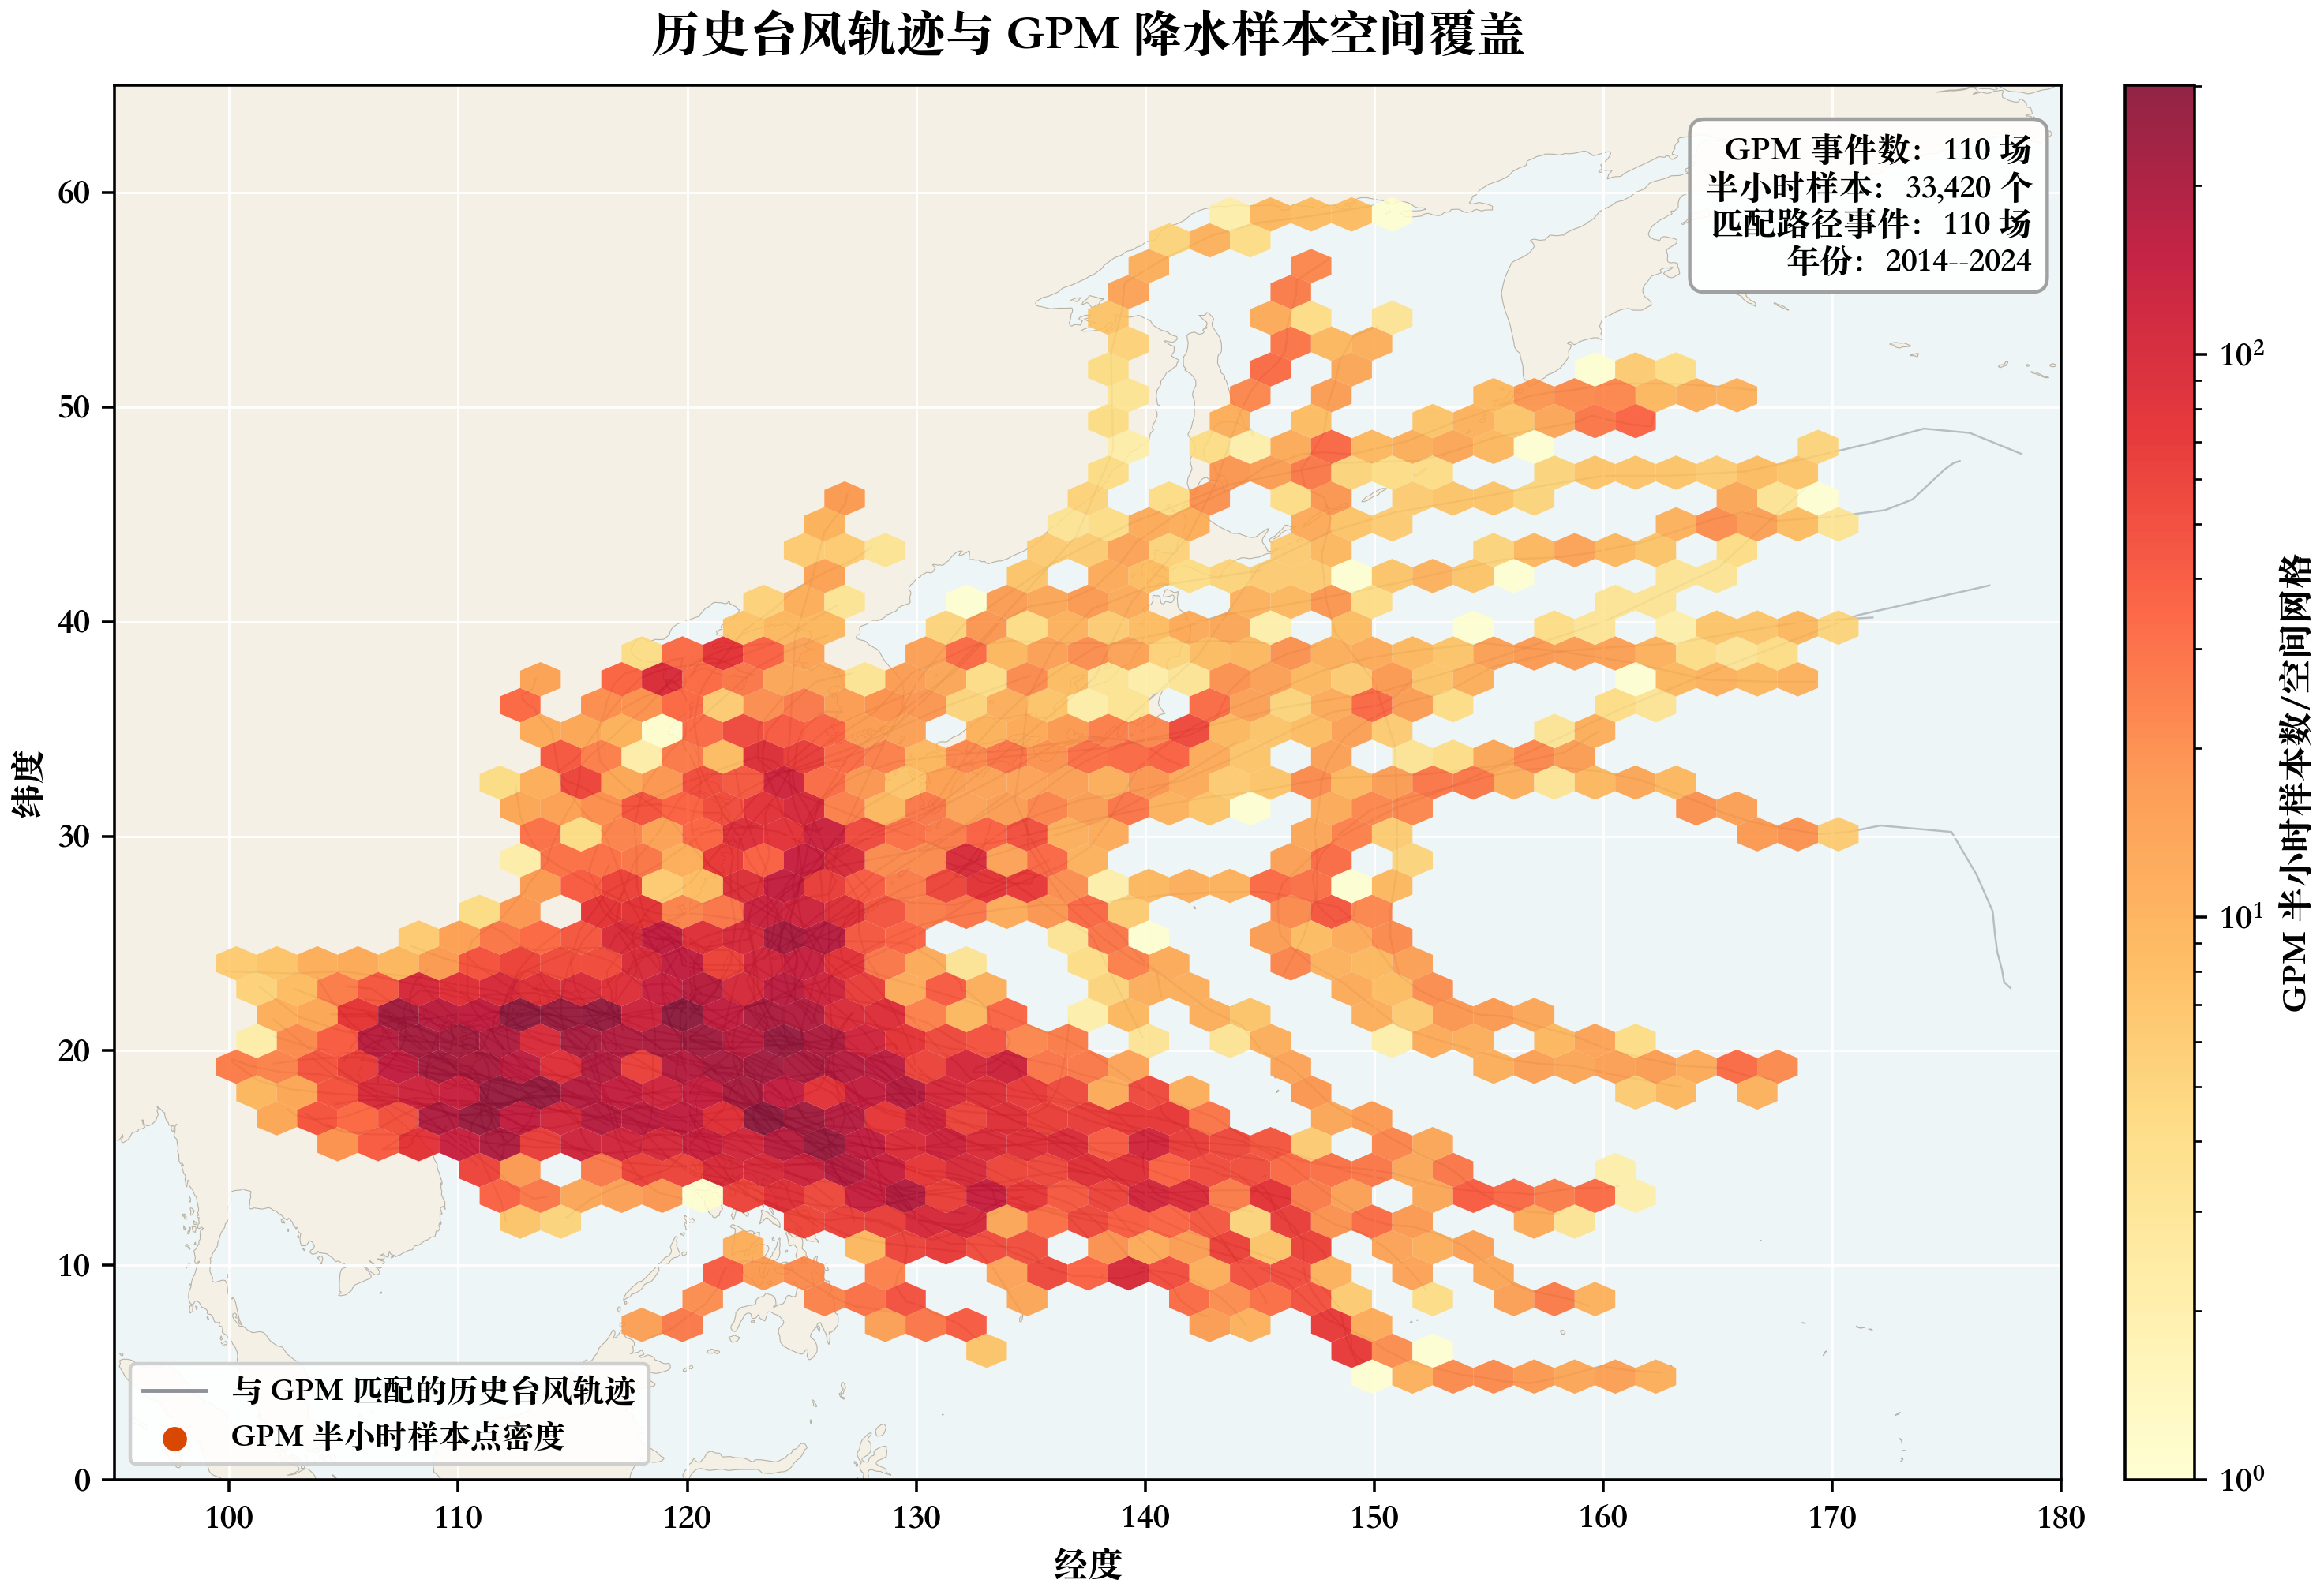
\includegraphics[width=0.95\textwidth]{outputs/figures/data_coverage/historical_tracks_gpm_sample_density.png}
  \caption{多场历史台风路径与 GPM 半小时降水样本空间覆盖示意}
  \label{fig:data_coverage_overview}
\end{figure}

\begin{table}[H]
  \centering
  \caption{数据来源与用途}
  \begin{tabularx}{\linewidth}{lXX}
    \toprule
    数据名称 & 主要字段 & 用途 \\
    \midrule
    CMABST台风路径资料 & 时间、经纬度、最大风速、中心气压、强度等级、距岸距离 & 构造路径、强度、移动和近岸环境解释变量 \\
    GPM半小时降水GeoTIFF & 半小时降水强度栅格、观测时间、台风中心与空间范围 & 提取降水强度、强降水面积、质心偏移和雨带结构指标 \\
    Natural Earth 陆地多边形数据 & land polygon & 计算台风中心邻域陆地覆盖比例 $landfrac\_200km$、$landfrac\_500km$ \\
    ETOPO 2022 全球地形起伏数据 & elevation / relief & 计算台风中心邻域地形平均高程、最大高程和地形起伏标准差 \\
    \bottomrule
  \end{tabularx}
\end{table}

\subsection{数据清洗与预处理}
\begin{enumerate}
  \item 路径时间对齐：将 CMABST 路径资料中的经度、纬度、中心气压、最大风速和距岸距离等连续变量插值到 GPM 半小时时刻，并利用 GPM 文件名中的台风中心位置进行中心误差校验。
  \item 降水栅格处理：读取 GPM 半小时 GeoTIFF 文件，统一空间坐标和单位口径，剔除无效值，并将雨强场转换到台风中心相对坐标系和台风相对运动坐标系中。
  \item 环境变量补充：基于 Natural Earth 陆地多边形计算台风中心邻域陆地覆盖比例和陆地判定变量，基于 ETOPO 2022 计算邻域平均高程、最大高程和地形起伏标准差。
  \item 安全输入构造：问题二和问题三仅使用路径、强度、移动、时间和近岸环境等可获得变量，不使用 \texttt{rain\_*}、\texttt{centroid\_*}、\texttt{quad\_*}、\texttt{rainband\_*} 等由真实降水场派生的泄漏变量。
  \item 标准化处理：历史相似样本检索中的连续变量均使用历史样本库的均值和标准差进行标准化，移动方向使用正弦和余弦表示，以避免角度循环误差。
\end{enumerate}

\subsection{指标体系构建}
\begin{table}[H]
  \centering
  \caption{台风降水空间结构指标体系}
  \begin{tabularx}{\linewidth}{lXlX}
    \toprule
    指标类别 & 指标名称 & 记号 & 计算方法 / 含义 \\
    \midrule
    强度类 & 最大雨强、分位雨强 & $R_{\max},R_{95},R_{99}$ & 描述单时次降水强度和极端尾部水平 \\
    范围类 & 强降水面积 & $A_{10},A_{20}$ & 统计雨强不低于给定阈值的格点面积 \\
    位置类 & 降水质心偏移 & $\Delta x,\Delta y$ & 计算降水质心相对台风中心的东西、南北偏移 \\
    非对称类 & 前后、左右及象限贡献 & $Q_F,Q_B,Q_L,Q_R$ & 在台风相对运动坐标系下统计各区域降水贡献 \\
    形态类 & 雨带各向异性、主轴长度与带宽 & $\kappa,L,B$ & 由降水加权协方差矩阵特征值计算，刻画雨带拉伸方向、主轴尺度和横向宽度 \\
    持续类 & 强降水持续时间 & $D_{10}$ & 统计固定地理格点达到强降水阈值的累计时长 \\
    \bottomrule
  \end{tabularx}
\end{table}

全文技术路线可概括为：首先完成路径资料与 GPM 降水资料的半小时时间对齐，并构造降水空间结构指标；其次在问题一中建立路径、强度、移动和环境变量对降水结构的解释模型；随后在问题二中基于安全输入检索相似历史模板，生成 KONG-REY 和 MAN-YI 的可能降水场；最后在问题三中对路径、强度和移动速度施加情景扰动，分析未来虚拟台风极端降水风险变化。

\section{问题一模型的建立与求解}

\subsection{模型思路}

问题一要求分析台风路径特征、强度特征与台风降水空间分布之间的关系。由于台风降水并非简单围绕台风中心对称分布，仅使用最大降水量或经纬度图难以刻画其空间结构。因此，本文从“路径--强度--移动--季节--海陆覆盖--地形环境--降水结构”的角度建立问题一模型。

具体而言，本文首先读取GPM半小时降水GeoTIFF文件，逐帧解析观测时间、台风中心位置和空间范围，并从降水栅格矩阵中提取降水强度、强降水范围、降水质心偏移、非对称性和雨带形态等指标。其次，由于CMABST路径资料时间分辨率低于GPM半小时降水资料，本文将台风路径中心、中心气压、最大风速和距岸距离等变量插值到每个GPM半小时时刻，并利用GPM文件名中给出的台风中心位置对插值结果进行误差校验。进一步地，本文根据题目要求自行补充 Natural Earth 陆地多边形数据和 ETOPO 2022 全球地形起伏数据，构造台风中心邻域陆地覆盖比例和地形起伏指标，从而辅助刻画海陆分布和地形抬升对台风降水空间结构的调制作用。最后，本文建立Spearman相关性分析和增强随机森林解释模型，定量分析路径、强度、移动、季节、海陆覆盖和地形环境对台风降水分布的影响。

此外，为进一步刻画台风降水相对于移动方向的空间偏向，本文不直接在经纬度坐标下分析降水场，而是建立以台风中心为原点、以台风移动方向为参考轴的台风相对运动坐标系，逐格计算前方、后方、左侧、右侧及四象限降水比例和强降水面积，从而更准确地刻画降水中心偏向、非对称性和雨带结构。

\subsection{路径数据与GPM降水数据的时间对齐}

GPM降水资料为半小时一帧，而CMABST路径资料通常不是半小时一条记录。若直接采用最近路径点匹配，会导致台风中心、强度和移动方向在半小时尺度上出现时间错位。为此，本文将路径资料插值到每一个GPM时刻。

设某场台风在路径资料中相邻两个时刻为$t_i$和$t_{i+1}$，对应的连续变量为$z_i$和$z_{i+1}$，其中$z$可表示经度、纬度、中心气压、最大风速或距岸距离等变量。对于任意GPM时刻$t\in[t_i,t_{i+1}]$，采用线性插值得到
\begin{equation}
    \hat{z}(t)=z_i+\frac{z_{i+1}-z_i}{t_{i+1}-t_i}(t-t_i).
\end{equation}

对于台风名称、编号、强度等级等离散变量，本文采用最近路径点赋值。对于经度变量，为避免跨越$180^\circ$经线时出现跳变，本文先对经度角度进行展开，再进行线性插值，最后归一化到$[-180^\circ,180^\circ]$范围内。

插值完成后，利用GPM文件名中给出的台风中心$(\lambda_t^G,\varphi_t^G)$与插值得到的路径中心$(\hat{\lambda}_t,\hat{\varphi}_t)$进行误差校验。中心误差采用Haversine球面距离：
\begin{equation}
    e_t=d_H\left((\lambda_t^G,\varphi_t^G),(\hat{\lambda}_t,\hat{\varphi}_t)\right).
\end{equation}

本文共对33420个GPM半小时时次完成路径插值匹配。校验结果如表\ref{tab:interp_quality_problem1}所示，所有样本均通过校验，中心误差均值为$0.331$ km，中位数为$0.371$ km，最大误差仅为$0.785$ km，说明插值得到的CMABST路径中心与GPM文件名中的台风中心高度一致。

\begin{table}[htbp]
    \centering
    \caption{路径插值到GPM半小时时刻后的中心误差校验}
    \label{tab:interp_quality_problem1}
    \begin{tabular}{ccccc}
        \hline
        样本数 & 正常匹配数 & 平均误差/km & 中位误差/km & 最大误差/km \\
        \hline
        33420 & 33420 & 0.331 & 0.371 & 0.785 \\
        \hline
    \end{tabular}
\end{table}

需要注意的是，GPM栅格值单位为$\mathrm{mm/hr}$，但每一帧代表半小时降水快照。因此，若某一时刻某格点降水强度为$R_t(x,y)$，则该半小时实际累计降水量为$0.5R_t(x,y)$。全过程累计降水应按
\begin{equation}
    P_{\mathrm{sum}}(x,y)=\sum_t 0.5R_t(x,y)
\end{equation}
计算。本文在问题一中主要分析半小时降水强度口径下的$R_t(x,y)$，因此$rain\_max$、$rain\_p95$等指标单位为$\mathrm{mm/hr}$；而$rain\_area\_10$表示降水强度不低于$10\ \mathrm{mm/hr}$的区域，等价于该半小时累计降水不低于$5\ \mathrm{mm}$的区域。

\subsection{降水分布特征指标体系}

设某一GPM时刻的降水强度场为$R_t(x_i,y_i)$，其中$(x_i,y_i)$为第$i$个格点的空间位置。本文从降水强度、强降水范围、降水质心偏移、固定地理方向非对称性、台风相对运动坐标系非对称性和雨带形态六个方面构建降水分布指标体系。

\subsubsection{台风中心相对坐标系}

虽然GPM降水栅格文件的空间边界已经随台风中心移动，但不同台风、不同时刻的经纬度位置不能直接用于比较降水结构。为统一刻画台风中心附近的降水空间分布，本文首先建立以台风中心为原点的局地相对坐标系。

设某一时刻台风中心经纬度为$(\lambda_c,\varphi_c)$，任一降水格点经纬度为$(\lambda,\varphi)$，则将经纬度差近似转换为以千米为单位的局地平面坐标：
\begin{equation}
    x=111\cos(\varphi_c)(\lambda-\lambda_c),
    \qquad
    y=111(\varphi-\varphi_c).
\end{equation}
其中，$x$轴正方向为正东，$y$轴正方向为正北，单位均为km。该坐标系将不同台风时刻的降水场统一到以台风中心为原点的相对空间中，便于比较降水中心偏移、降水半径和雨带形态。

\subsubsection{台风相对运动坐标系}

为了进一步分析降水结构相对于台风移动方向的前后与左右偏向，本文在台风中心相对坐标系的基础上构建台风相对运动坐标系。设台风移动方向方位角为$\alpha$，其中$\alpha=0^\circ$表示向北移动，$\alpha=90^\circ$表示向东移动，角度按顺时针方向增加。将局地坐标$(x,y)$投影到台风移动方向及其左侧法向方向，得到运动相对坐标：
\begin{equation}
    x'=x\sin\alpha+y\cos\alpha,
\end{equation}
\begin{equation}
    y'=-x\cos\alpha+y\sin\alpha.
\end{equation}

其中，$x'>0$表示格点位于台风移动前方，$x'<0$表示位于后方；$y'>0$表示位于移动方向左侧，$y'<0$表示位于右侧。由此可定义前方、后方、左侧和右侧区域：
\begin{equation}
    \Omega_F=\{(x',y'):x'>0\},\quad
    \Omega_B=\{(x',y'):x'<0\},
\end{equation}
\begin{equation}
    \Omega_L=\{(x',y'):y'>0\},\quad
    \Omega_R=\{(x',y'):y'<0\}.
\end{equation}

进一步定义四个相对运动象限：
\begin{equation}
    \Omega_{FL}=\{x'>0,y'>0\},\quad
    \Omega_{FR}=\{x'>0,y'<0\},
\end{equation}
\begin{equation}
    \Omega_{BL}=\{x'<0,y'>0\},\quad
    \Omega_{BR}=\{x'<0,y'<0\}.
\end{equation}
其中，$\Omega_{FR}$表示右前象限，$\Omega_{BL}$表示左后象限。

\subsubsection{降水强度特征}

为描述降水强度，本文计算降水场最大值、分位数和均值。重点使用最大降水强度$R_{\max}$和95分位数降水强度$R_{95}$：
\begin{equation}
    R_{\max,t}=\max_i R_t(x_i,y_i),
\end{equation}
\begin{equation}
    R_{95,t}=\mathrm{Quantile}_{0.95}\{R_t(x_i,y_i)\}.
\end{equation}
其中，$R_{\max}$反映局地极端降水峰值，$R_{95}$反映更稳定的强降水水平。

\subsubsection{强降水范围特征}

设$A_i$为第$i$个格点面积。由于GPM空间分辨率约为$0.1^\circ\times0.1^\circ$，本文按中心纬度修正格点面积：
\begin{equation}
    A_i \approx 11.1\times 11.1 \times \cos(\varphi_c)\quad(\mathrm{km^2}).
\end{equation}
定义降水强度不低于$10\ \mathrm{mm/hr}$的强降水面积为
\begin{equation}
    A_{10,t}=\sum_i A_i\mathbf{1}\{R_t(x_i,y_i)\geq 10\}.
\end{equation}
该指标等价于半小时累计降水不低于$5\ \mathrm{mm}$的区域面积。为便于解释，进一步定义强降水等效半径：
\begin{equation}
    r_{10,t}^{eq}=\sqrt{\frac{A_{10,t}}{\pi}}.
\end{equation}

\subsubsection{降水质心偏移特征}

在台风中心相对坐标系下，以降水强度为权重，定义降水质心：
\begin{equation}
    \bar{x}_t=\frac{\sum_i R_t(x_i,y_i)x_i}{\sum_i R_t(x_i,y_i)},\qquad
    \bar{y}_t=\frac{\sum_i R_t(x_i,y_i)y_i}{\sum_i R_t(x_i,y_i)}.
\end{equation}
其中，$x_i$和$y_i$分别表示第$i$个格点相对于台风中心的东西向和南北向距离，单位为km。因此，降水质心偏移距离可直接用平面距离表示为
\begin{equation}
    D_{c,t}=\sqrt{\bar{x}_t^2+\bar{y}_t^2}.
\end{equation}

若需要刻画降水质心偏移方向，则定义
\begin{equation}
    \theta_{c,t}=\operatorname{atan2}(\bar{y}_t,\bar{x}_t).
\end{equation}
其中，$\theta_{c,t}$为相对于正东方向的数学角，逆时针为正。进一步将其与台风移动方向进行比较，即可得到降水质心相对于台风运动方向的偏移角，用于判断降水中心偏向移动前方、后方、左侧或右侧。

\subsubsection{固定地理方向非对称性特征}

在台风相对坐标系下，本文首先从固定地理方向定义东西、南北非对称性。以台风中心为分界，定义东西方向非对称性：
\begin{equation}
    S_{EW,t}=
    \frac{\sum_{x_i\geq x_{c,t}}R_t(x_i,y_i)-\sum_{x_i<x_{c,t}}R_t(x_i,y_i)}
    {\sum_i R_t(x_i,y_i)}.
\end{equation}
类似地，定义南北方向非对称性：
\begin{equation}
    S_{NS,t}=
    \frac{\sum_{y_i\geq y_{c,t}}R_t(x_i,y_i)-\sum_{y_i<y_{c,t}}R_t(x_i,y_i)}
    {\sum_i R_t(x_i,y_i)}.
\end{equation}
其中，$S_{EW}>0$表示降水偏向台风中心东侧，$S_{EW}<0$表示偏向西侧；$S_{NS}>0$表示偏向北侧，$S_{NS}<0$表示偏向南侧。

\subsubsection{运动相对非对称性特征}

在台风相对运动坐标系下，以降水强度$R_i$为权重，定义前方、后方、左侧和右侧降水比例：
\begin{equation}
    Q_F=\frac{\sum_{(x'_i,y'_i)\in\Omega_F}R_i}{\sum_i R_i},
    \qquad
    Q_B=\frac{\sum_{(x'_i,y'_i)\in\Omega_B}R_i}{\sum_i R_i},
\end{equation}
\begin{equation}
    Q_L=\frac{\sum_{(x'_i,y'_i)\in\Omega_L}R_i}{\sum_i R_i},
    \qquad
    Q_R=\frac{\sum_{(x'_i,y'_i)\in\Omega_R}R_i}{\sum_i R_i}.
\end{equation}

前后非对称性和左右非对称性分别定义为：
\begin{equation}
    A_{FB}=
    \frac{
    \sum_{(x'_i,y'_i)\in\Omega_F}R_i-
    \sum_{(x'_i,y'_i)\in\Omega_B}R_i
    }{\sum_i R_i},
\end{equation}
\begin{equation}
    A_{LR}=
    \frac{
    \sum_{(x'_i,y'_i)\in\Omega_L}R_i-
    \sum_{(x'_i,y'_i)\in\Omega_R}R_i
    }{\sum_i R_i}.
\end{equation}
其中，$A_{FB}>0$表示降水偏向台风移动前方，$A_{LR}>0$表示降水偏向台风移动方向左侧。由于比例型指标分子和分母同时使用$R_i$，若改用半小时累计雨量$0.5R_i$，常数因子会同时抵消，因此不影响比例和非对称性指标的计算。

进一步地，本文还计算四象限降水比例，以及运动坐标系下前方、后方、左侧、右侧的$10\ \mathrm{mm/hr}$以上强降水面积，用于刻画强降水区相对于台风移动方向的位置。

\subsubsection{雨带形态特征}

为描述降水带是否呈狭长形态，本文将格点经纬度近似转换为以台风中心为原点的局地平面坐标，并以降水强度为权重计算二维协方差矩阵$\Sigma_t$。设$\lambda_{1,t}\geq\lambda_{2,t}$为$\Sigma_t$的两个特征值，则定义雨带各向异性指数：
\begin{equation}
    \eta_t=\frac{\sqrt{\lambda_{1,t}}-\sqrt{\lambda_{2,t}}}
    {\sqrt{\lambda_{1,t}}+\sqrt{\lambda_{2,t}}}.
\end{equation}
当$\eta_t$接近0时，降水分布接近圆形；当$\eta_t$较大时，降水带呈更明显的狭长结构。进一步地，本文计算雨带主轴方向与台风移动方向之间的夹角，用于刻画降水带相对于台风运动方向的伸展关系。

为进一步刻画题目要求中的降水带宽，本文在台风相对运动坐标系下取有效降水格点集合
\[
    \Omega_t=\{i:R_i\geq 1.0\ \mathrm{mm/hr},\ R_i\ \mathrm{finite}\},
\]
并以雨强 $w_i=R_i$ 为权重计算降水加权协方差矩阵 $\Sigma_t$。若有效格点少于5个或总权重不为正，则该时次带宽记为缺失。设 $\Sigma_t$ 的特征值为 $\lambda_{1,t}\geq\lambda_{2,t}$，本文定义雨带主轴等效长度和横向等效带宽为
\[
    L_t=4\sqrt{\lambda_{1,t}},\qquad
    B_t=4\sqrt{\lambda_{2,t}}.
\]
其中 $B_t$ 越大，表示主要降水带在垂直主轴方向上的扩展越宽；在相同强降水面积下，较小的 $B_t$ 往往对应更狭长集中的雨带，较大的 $B_t$ 则表示降水横向铺展更明显。系数4对应约 $\pm2\sigma$ 范围内的等效尺度。作为极端雨带诊断，本文还在 $R_i\geq10\ \mathrm{mm/hr}$ 的强降水格点上计算 $B_{10,t}=4\sqrt{\lambda_{2,t}^{(10)}}$。

\subsection{路径、强度与环境解释变量构造}

在路径和强度特征方面，本文使用台风最大风速$V_t$、中心气压$P_t$、移动速度$U_t$、移动方向$\alpha_t$等变量。由于移动方向是周期变量，直接作为数值变量会导致$359^\circ$与$1^\circ$在数值上相差很大但实际方向接近的问题。因此，本文将移动方向转化为正弦和余弦形式：
\begin{equation}
    M_{\sin,t}=\sin\left(\frac{\pi\alpha_t}{180}\right),\qquad
    M_{\cos,t}=\cos\left(\frac{\pi\alpha_t}{180}\right).
\end{equation}

为综合描述台风强度，构造气压亏损量：
\begin{equation}
    \Delta P_t=\bar{P}-P_t,
\end{equation}
其中$\bar{P}$为样本平均中心气压。再将最大风速和气压亏损标准化，得到综合强度指数：
\begin{equation}
    I_t=\frac{1}{2}Z(V_t)+\frac{1}{2}Z(\Delta P_t).
\end{equation}
其中$Z(\cdot)$表示标准化处理。$I_t$越大，表示台风强度越强。

在海陆环境方面，使用距岸距离$d_t$、有符号距岸距离$d_t^s$、是否登陆标记$I_t^{land}$及近岸影响指数：
\begin{equation}
    C_t=\exp\left(-\frac{|d_t|}{200}\right).
\end{equation}
其中，$C_t$越大表示台风中心越接近海岸线，海陆热力差异、陆面摩擦和地形抬升对降水分布的调制可能越明显。

为进一步刻画台风中心附近的海陆覆盖和地形起伏，本文补充 Natural Earth 陆地多边形数据和 ETOPO 2022 全球地形起伏数据，构造陆地覆盖比例与地形统计量。设 $\Omega_R(t)$ 为以第 $t$ 个台风中心为圆心、半径 $R$ km 的邻域，$I_i^{land}$ 表示第 $i$ 个采样点是否位于陆地，则定义
\[
F_{land,R}(t)=\frac{1}{N_R}\sum_{i\in\Omega_R(t)}I_i^{land}.
\]
本文取 $R=200$ km 和 $R=500$ km，分别得到 $landfrac\_200km$ 和 $landfrac\_500km$，用于刻画台风核心区和外围环流影响范围内的陆地覆盖比例。

设 $H_i$ 为陆地点高程，则定义
\[
\bar H_R(t)=\frac{1}{N_R}\sum_{i\in\Omega_R(t)}H_i,\quad
H_{max,R}(t)=\max_{i\in\Omega_R(t)}H_i,
\]
\[
H_{std,R}(t)=
\sqrt{\frac{1}{N_R}\sum_{i\in\Omega_R(t)}(H_i-\bar H_R(t))^2}.
\]
本文取 $R=300$ km，得到 $terrain\_mean\_300km$、$terrain\_max\_300km$ 和 $terrain\_std\_300km$，用于刻画台风中心附近地形抬升和地形起伏条件。

此外，为表征季节背景和日变化背景，本文构造月份和小时的周期特征：
\begin{equation}
    T_{\mathrm{month},\sin}=\sin\left(\frac{2\pi m}{12}\right),\quad
    T_{\mathrm{month},\cos}=\cos\left(\frac{2\pi m}{12}\right),
\end{equation}
\begin{equation}
    T_{\mathrm{hour},\sin}=\sin\left(\frac{2\pi h}{24}\right),\quad
    T_{\mathrm{hour},\cos}=\cos\left(\frac{2\pi h}{24}\right).
\end{equation}

综上，问题一中用于解释降水分布的主要变量包括台风强度、移动过程、强度变化率、海陆覆盖、距岸距离、地形起伏和时间背景等。主要变量如表\ref{tab:variables_problem1}所示。

\begin{table}[htbp]
    \centering
    \caption{问题一主要解释变量与响应变量}
    \label{tab:variables_problem1}
    \begin{tabular}{p{0.25\textwidth}p{0.65\textwidth}}
        \hline
        变量类别 & 具体变量 \\
        \hline
        强度变量 & 最大风速 WND、中心最低气压 PRES、气压亏损、强度等级、综合强度指数、风速变化率、气压变化率；由于 OWD 缺失，未构造风速半径变量。 \\
        移动变量 & 移动速度、移动方向正弦、移动方向余弦 \\
        演变变量 & 风速变化率、气压变化率、增强/减弱状态 \\
        海陆与地形变量 & 是否登陆、距岸距离、有符号距岸距离、近岸影响指数、200 km/500 km陆地覆盖比例、300 km邻域平均高程、最大高程、地形起伏标准差 \\
        时间背景 & 月份正弦、月份余弦、小时正弦、小时余弦 \\
        降水响应变量 & 最大降水强度、P95降水强度、强降水面积、强降水等效半径、降水质心偏移、东西/南北非对称性、前后/左右非对称性、四象限降水比例、雨带各向异性 \\
        \hline
    \end{tabular}
\end{table}

\subsection{路径--强度--环境与降水分布关系模型}

为从不同角度刻画台风因素与降水分布的关系，本文采用Spearman相关性分析和增强随机森林解释模型。

\subsubsection{Spearman相关性分析}

首先计算解释变量$X_j$与降水分布特征$Y_k$之间的Spearman秩相关系数：
\begin{equation}
    \rho_{jk}=\mathrm{corr}_{S}(X_j,Y_k).
\end{equation}
Spearman相关系数不要求变量满足线性关系，能够刻画单调相关性，适合初步分析台风因子与降水指标之间的方向性关系。本文将所有解释变量与降水响应变量之间的Spearman相关系数绘制成热力图，如图\ref{fig:spearman_heatmap_problem1}所示。

\begin{figure}[htbp]
    \centering
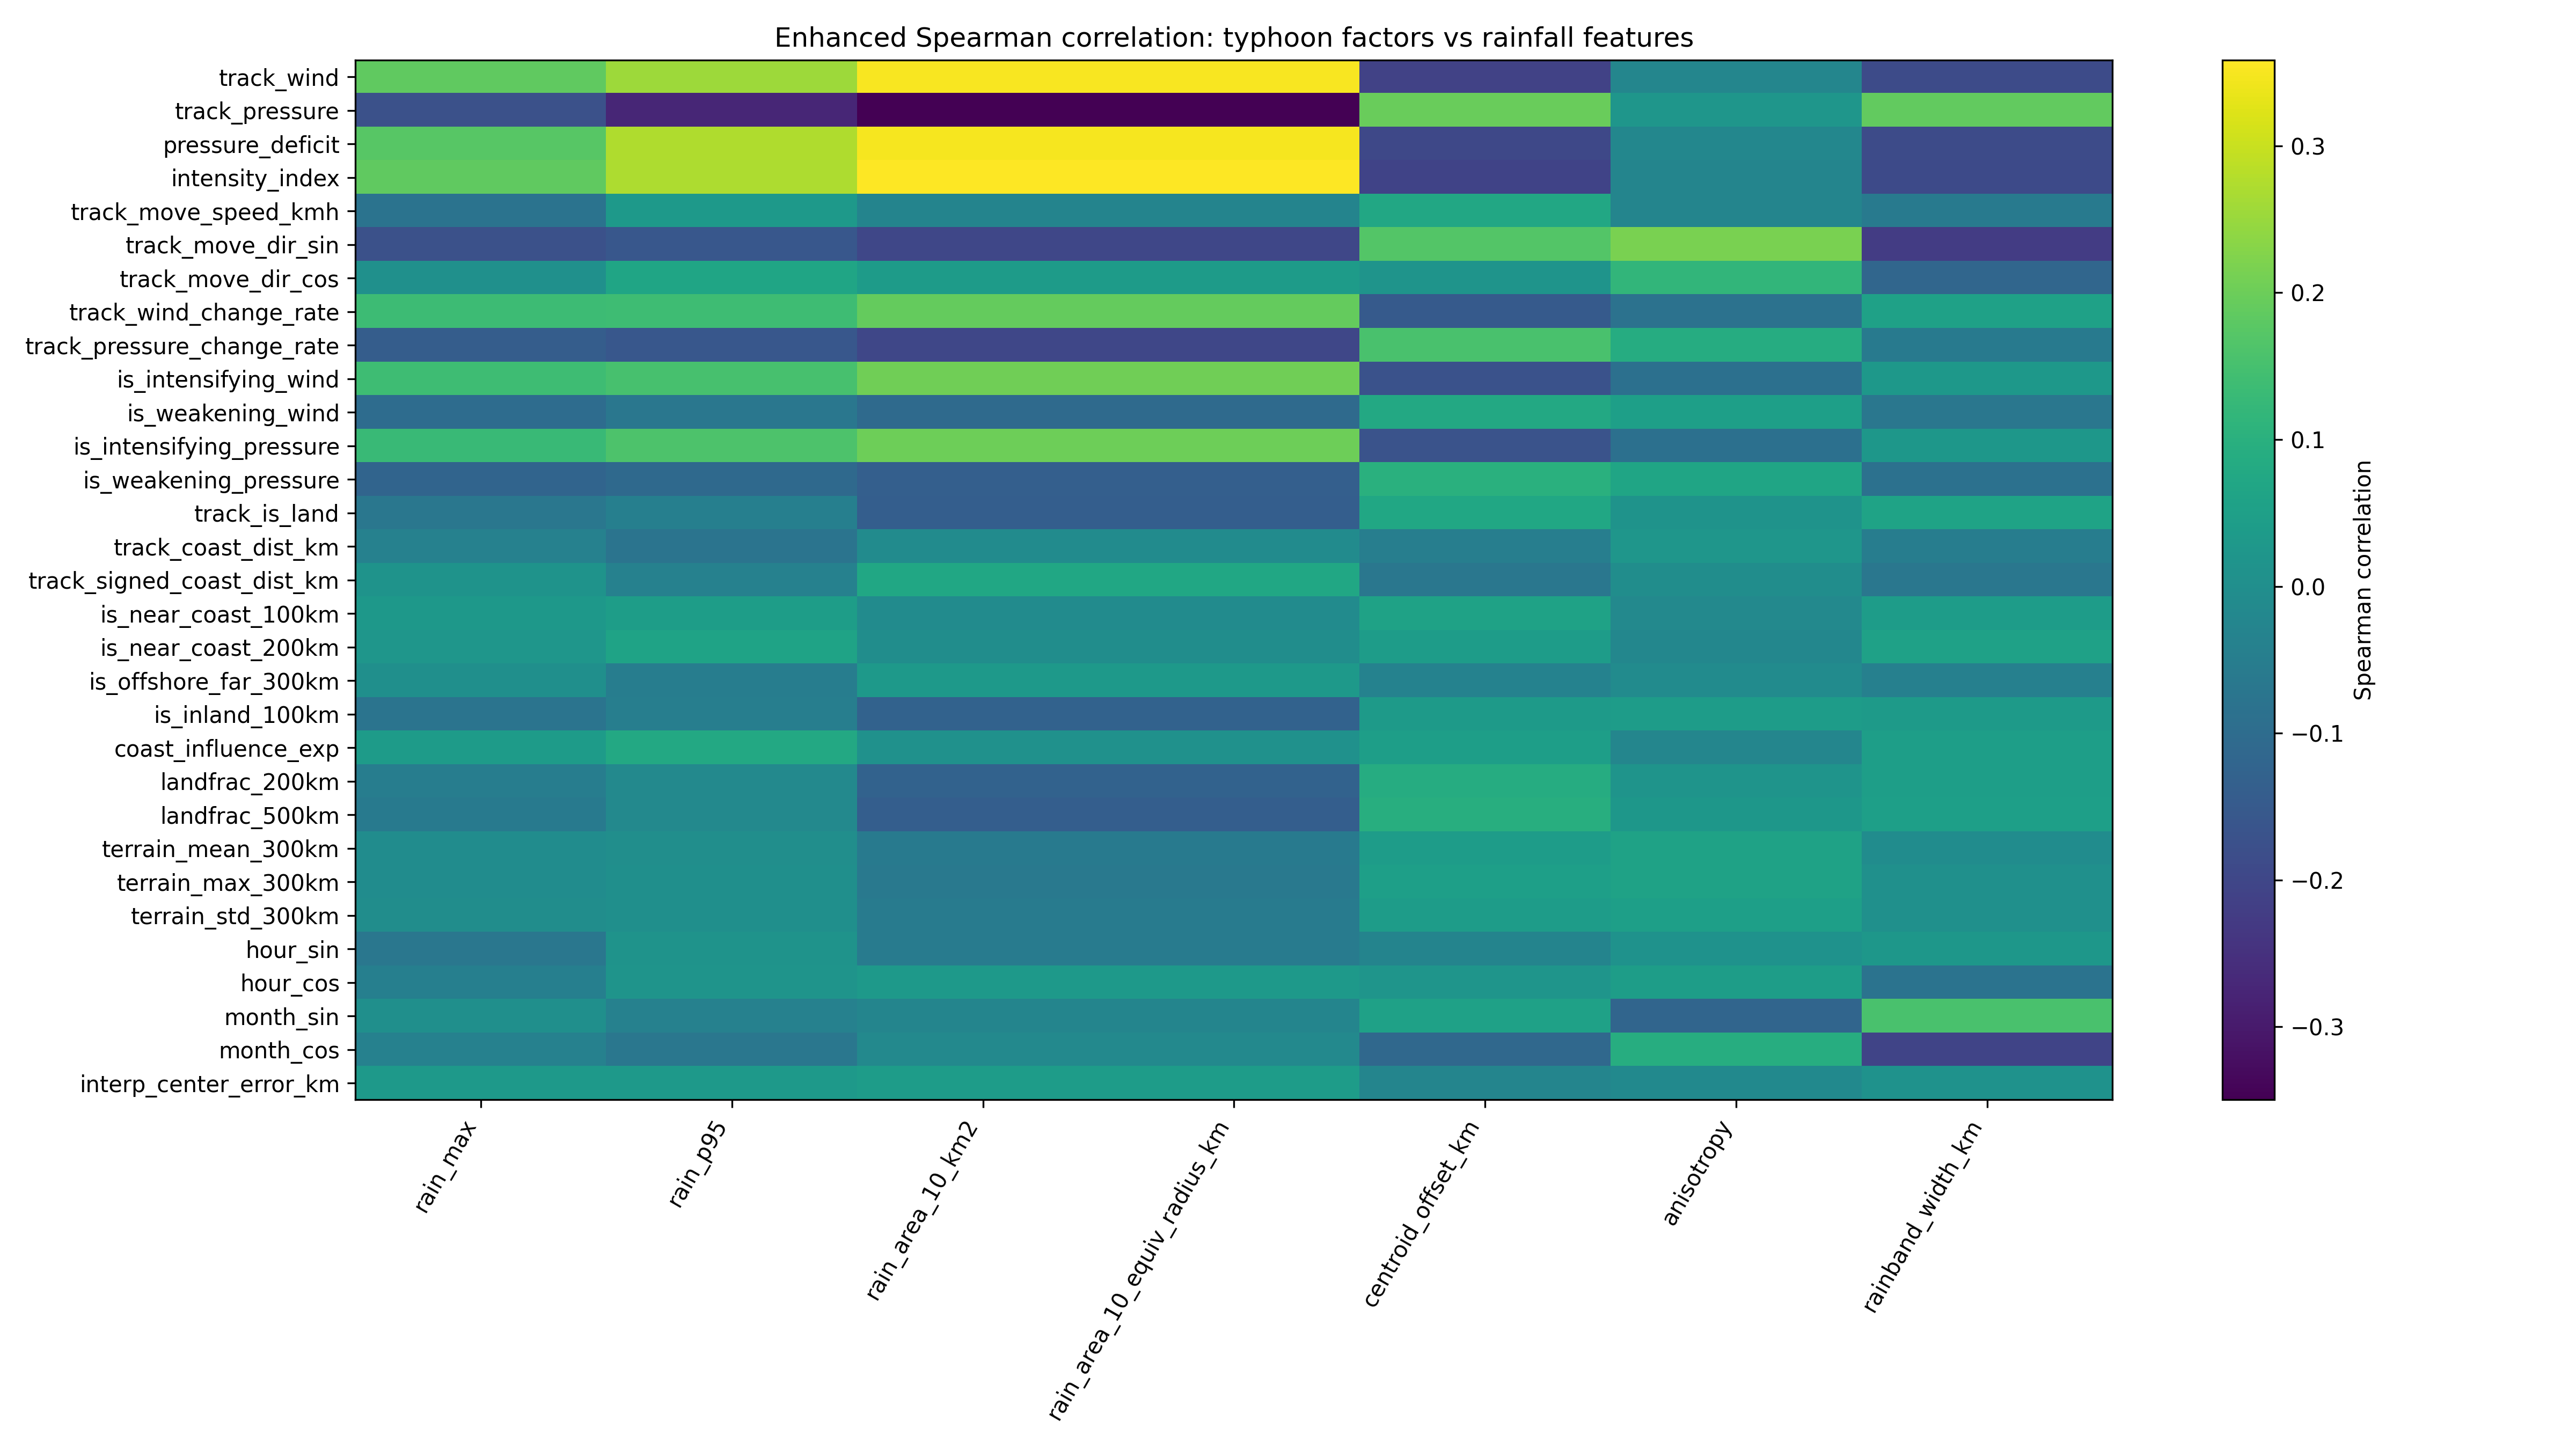
\includegraphics[width=0.95\textwidth]{outputs/figures/problem1_env/01_enhanced_spearman_heatmap.png}
    \caption{补充环境变量后路径、强度、环境因子与降水分布特征的Spearman相关性热力图}
    \label{fig:spearman_heatmap_problem1}
\end{figure}

\subsubsection{增强随机森林解释模型}

由于台风降水分布受多因素共同影响，且变量之间可能存在非线性关系，本文进一步建立增强随机森林回归模型。对每一个降水响应变量$Y_k$，以路径、强度、移动、季节、海陆覆盖和地形环境变量组成特征向量$\mathbf{X}_t$，建立模型：
\begin{equation}
    Y_{k,t}=f_k(\mathbf{X}_t)+\varepsilon_t.
\end{equation}
其中$f_k(\cdot)$由随机森林模型拟合，$\varepsilon_t$为残差项。本文使用的随机森林主要参数为：树数量$n_{\mathrm{estimators}}=250$，最大深度$max\_depth=14$，叶节点最小样本数$min\_samples\_leaf=20$。训练集和测试集按$3:1$随机划分，并采用置换重要性衡量不同解释变量对目标变量的贡献。

随机森林置换重要性定义为：在测试集上随机打乱某一特征后，模型预测性能下降的幅度。若某变量被打乱后模型性能下降越大，则说明该变量对解释目标降水特征越重要。

\subsection{模型求解结果}

\subsubsection{模型总体拟合效果}

基于插值后的半小时路径--降水联合样本，本文对六个主要降水响应变量分别建立增强随机森林模型。模型测试集$R^2$结果如表\ref{tab:rf_r2_problem1}所示。

\begin{table}[htbp]
    \centering
    \caption{增强随机森林模型对主要降水分布特征的解释效果}
    \label{tab:rf_r2_problem1}
    \begin{tabular}{lcc}
        \hline
        响应变量 & 含义 & 测试集$R^2$ \\
        \hline
        $rain\_max$ & 单点最大降水强度 & 0.409 \\
        $rain\_p95$ & P95降水强度 & 0.666 \\
        $rain\_area\_10\_km^2$ & 强降水面积 & 0.614 \\
        $rain\_area\_10\_equiv\_radius$ & 强降水等效半径 & 0.665 \\
        $centroid\_offset$ & 降水质心偏移 & 0.684 \\
        $anisotropy$ & 雨带各向异性 & 0.640 \\
        \hline
    \end{tabular}
\end{table}

由表\ref{tab:rf_r2_problem1}可见，引入陆地覆盖比例和地形起伏变量后，模型对所有目标变量的解释能力均未下降，且对P95降水强度、强降水面积、强降水等效半径和降水质心偏移的解释效果均有一定提升，说明补充环境变量能够提供原有距岸距离无法完全刻画的下垫面信息。模型对P95降水强度、强降水等效半径、降水质心偏移和雨带各向异性的测试集$R^2$均超过0.64，说明路径、强度、移动、海陆、地形和季节背景特征能够较好解释台风降水空间结构的主要变化。相比之下，单点最大降水强度$rain\_max$的$R^2$为0.409，解释能力相对较弱。这主要是因为单点最大值更容易受到局地强对流、遥感反演误差和孤立极值格点影响，稳定性弱于分位数和面积类指标。

\subsubsection{台风强度对降水强度与强降水范围的影响}

由于路径数据中 OWD 缺失，本文无法直接分析风速半径对降水结构的影响。考虑到 WND 与 PRES 是 CMABSTdata 中最稳定的强度字段，本文以最大风速、中心最低气压、气压亏损和强度等级刻画台风强度，并进一步引入风速变化率和气压变化率刻画强度演变过程。

Spearman相关性结果显示，P95降水强度与中心气压呈负相关，与气压亏损、综合强度指数和最大风速呈正相关。其中，$rain\_p95$与中心气压的相关系数为$-0.274$，与气压亏损的相关系数为$0.274$，与综合强度指数的相关系数为$0.271$，与最大风速的相关系数为$0.254$。

对于强降水面积$rain\_area\_10\_km^2$，其与综合强度指数的相关系数为$0.358$，与最大风速的相关系数为$0.352$，与中心气压的相关系数为$-0.350$，与气压亏损的相关系数为$0.350$。这表明台风强度是降水强度和强降水范围的主控因子。中心气压越低、气压亏损越大、最大风速越高，台风的强降水水平和强降水覆盖范围越大。

图\ref{fig:intensity_p95_problem1}和图\ref{fig:intensity_area10_problem1}分别展示了综合强度指数与P95降水强度、强降水面积之间的关系。

\begin{figure}[htbp]
    \centering
    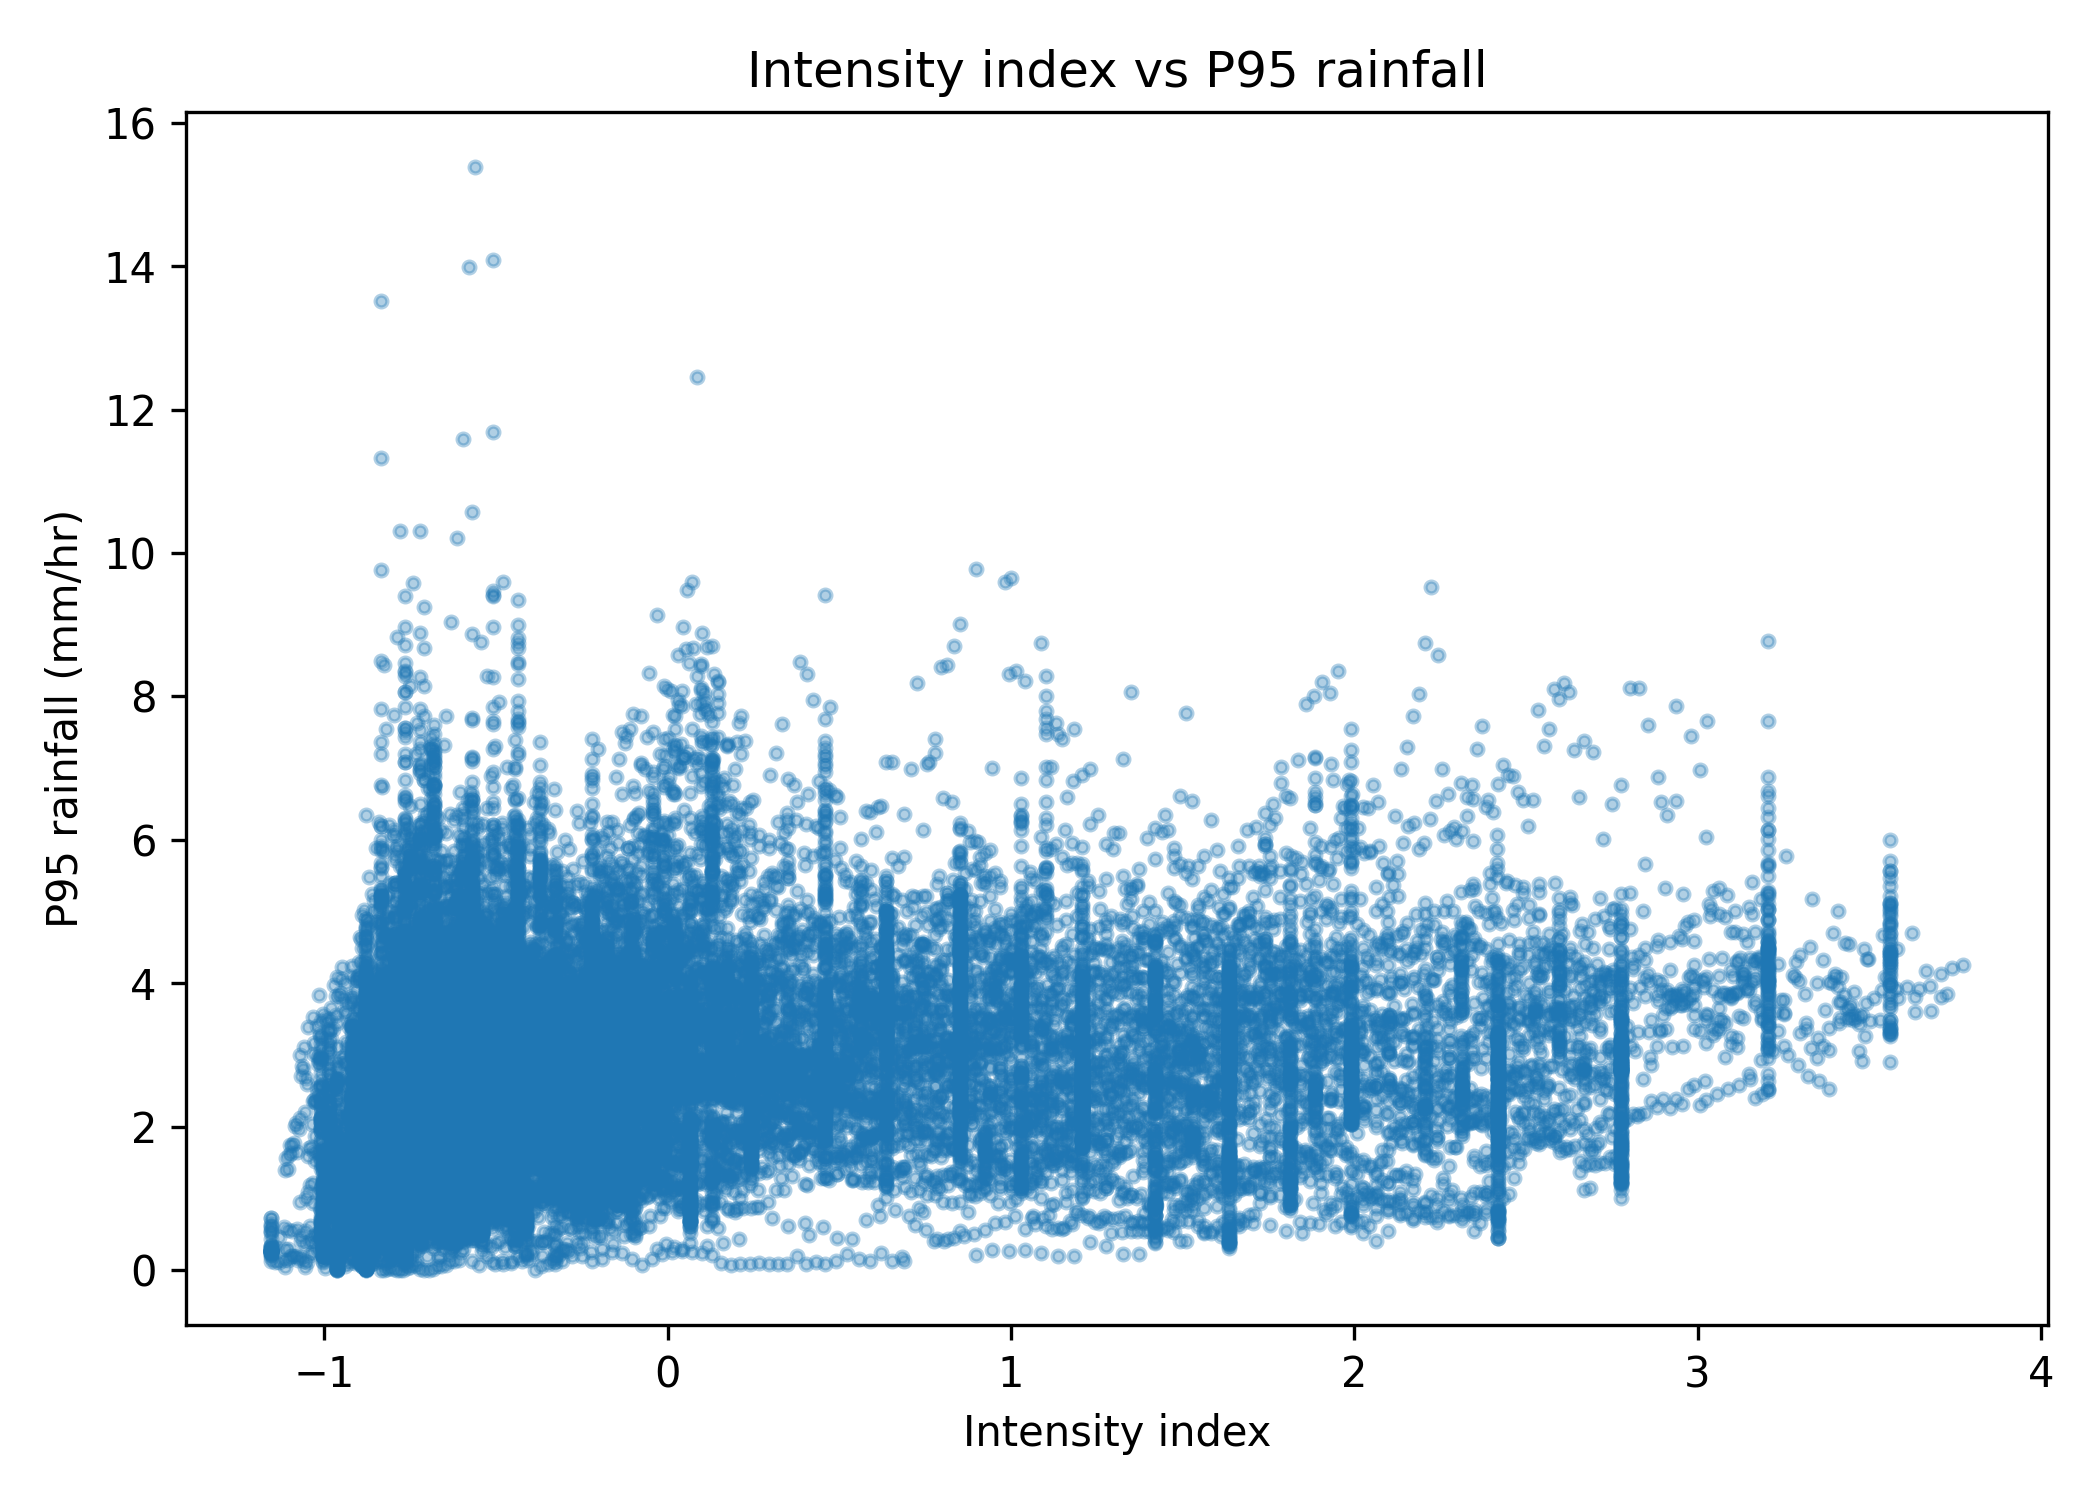
\includegraphics[width=0.72\textwidth]{outputs/figures/problem1_env/02_intensity_index_vs_rain_p95.png}
    \caption{补充环境变量后综合强度指数与P95降水强度的关系}
    \label{fig:intensity_p95_problem1}
\end{figure}

\begin{figure}[htbp]
    \centering
    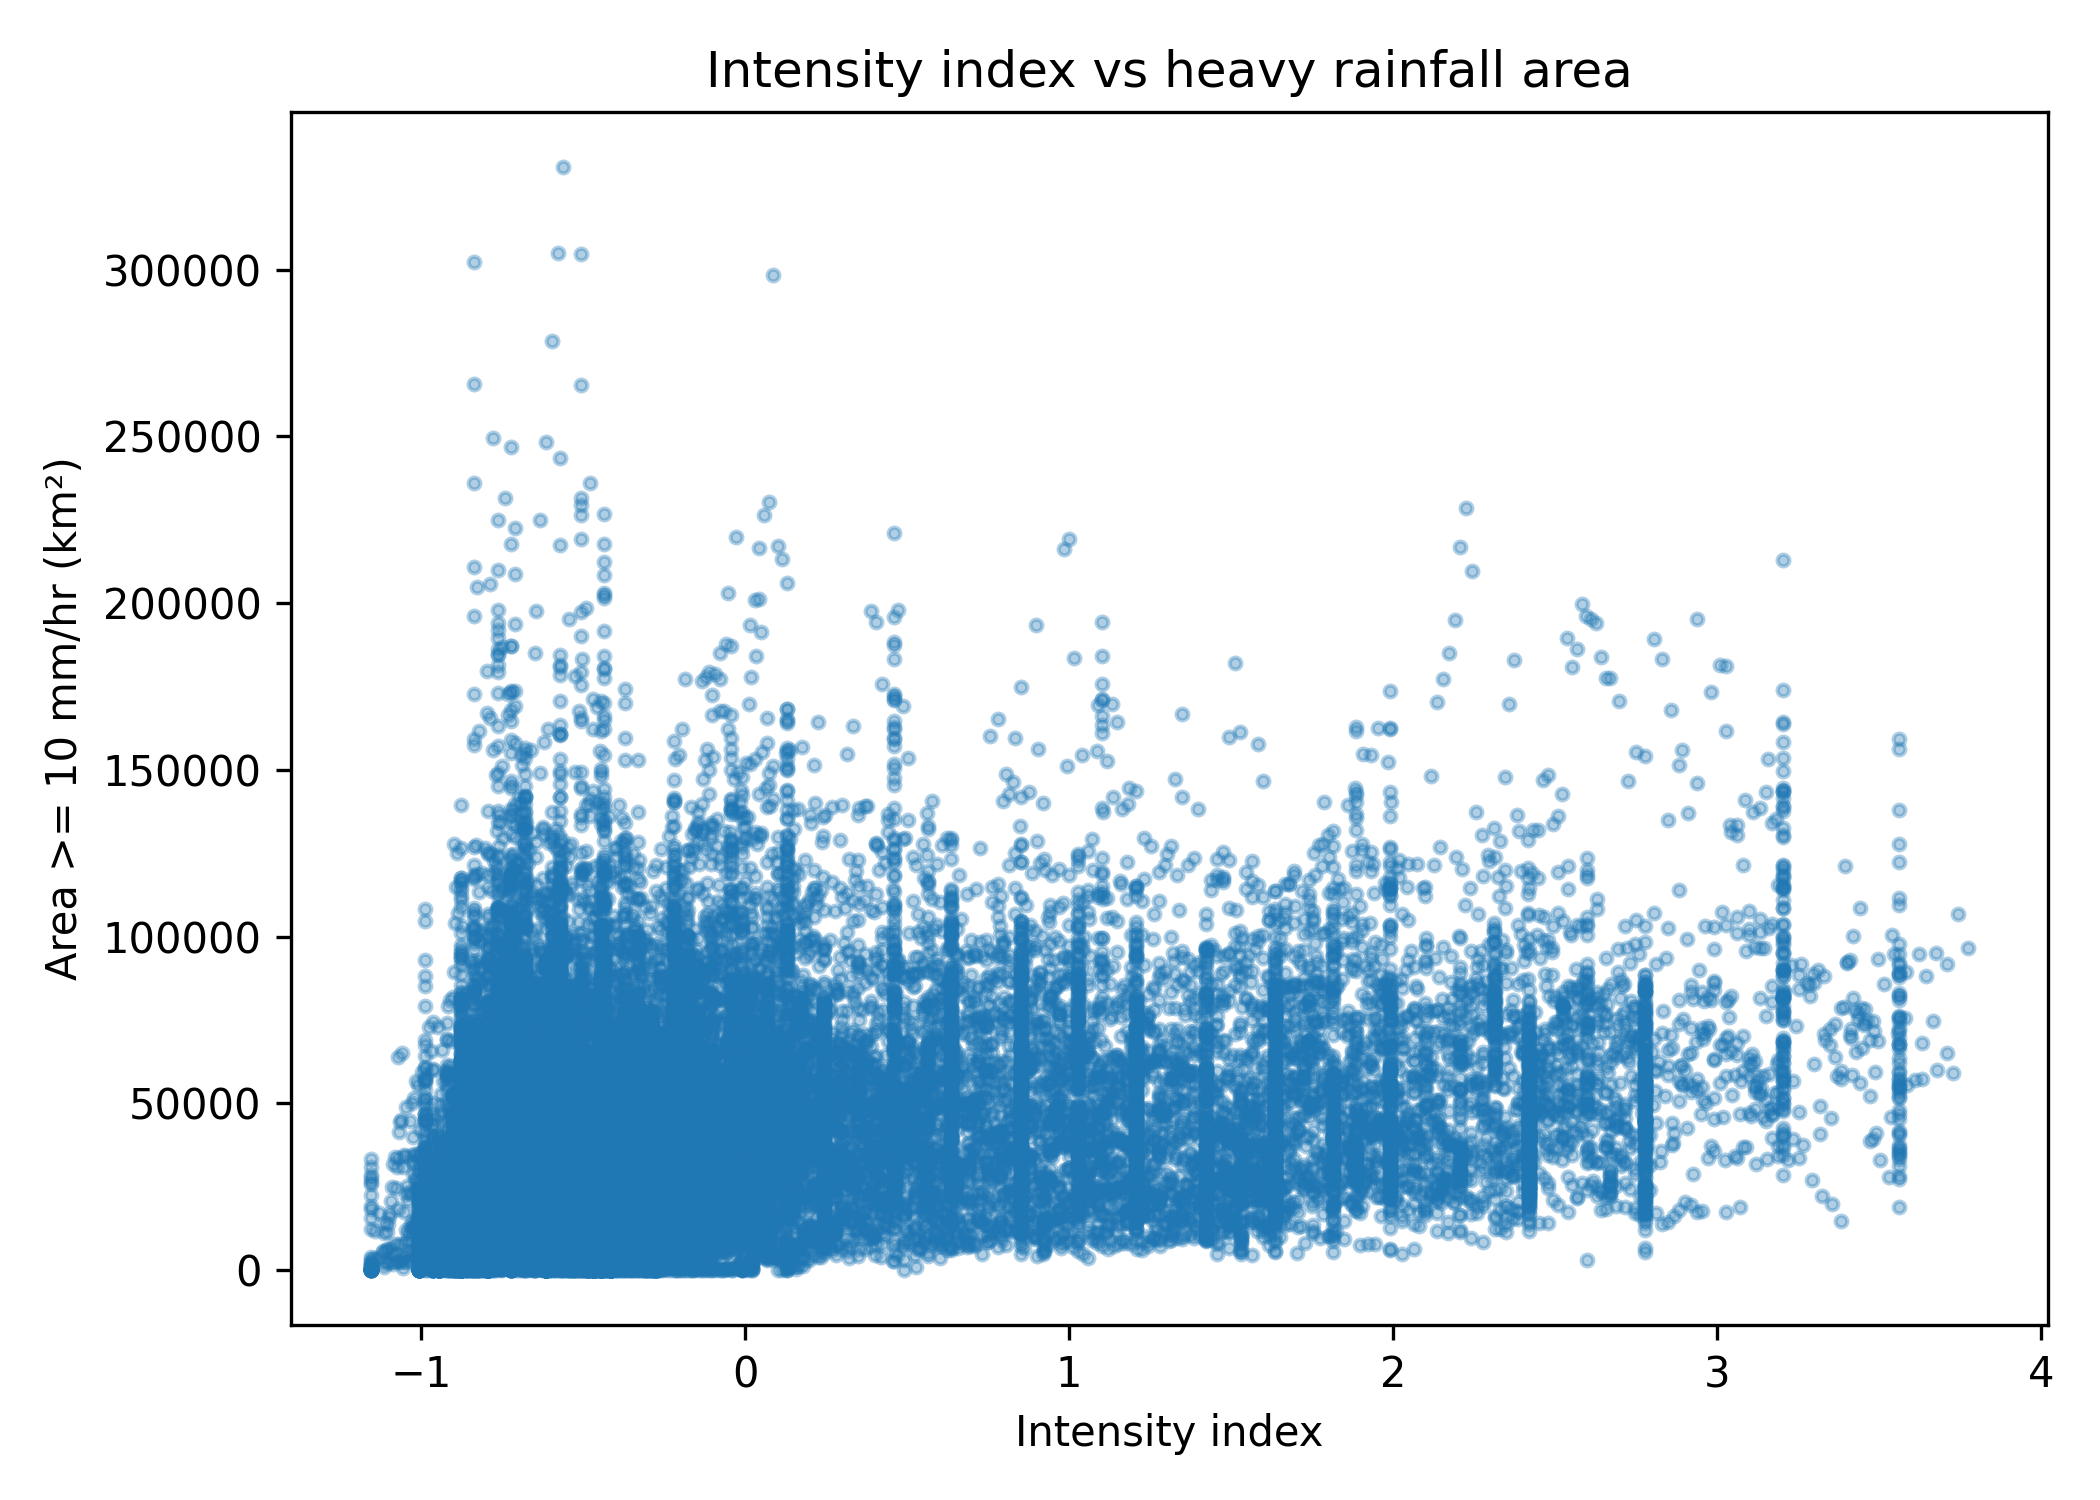
\includegraphics[width=0.72\textwidth]{outputs/figures/problem1_env/03_intensity_index_vs_area10_km2.png}
    \caption{补充环境变量后综合强度指数与强降水面积的关系}
    \label{fig:intensity_area10_problem1}
\end{figure}

随机森林置换重要性进一步支持上述结论。对于$rain\_p95$，移动方向正弦、月份余弦、综合强度指数、移动方向余弦和中心气压为前五个重要因素；对于$rain\_area\_10\_km^2$，移动方向正弦、最大风速、$landfrac\_500km$、气压亏损和移动方向余弦为前五个重要因素。虽然随机森林中的变量重要性体现了非线性和交互效应，但强度相关变量始终位于前列，同时较大尺度陆地覆盖比例也对强降水范围具有明显解释贡献。

\begin{figure}[htbp]
    \centering
    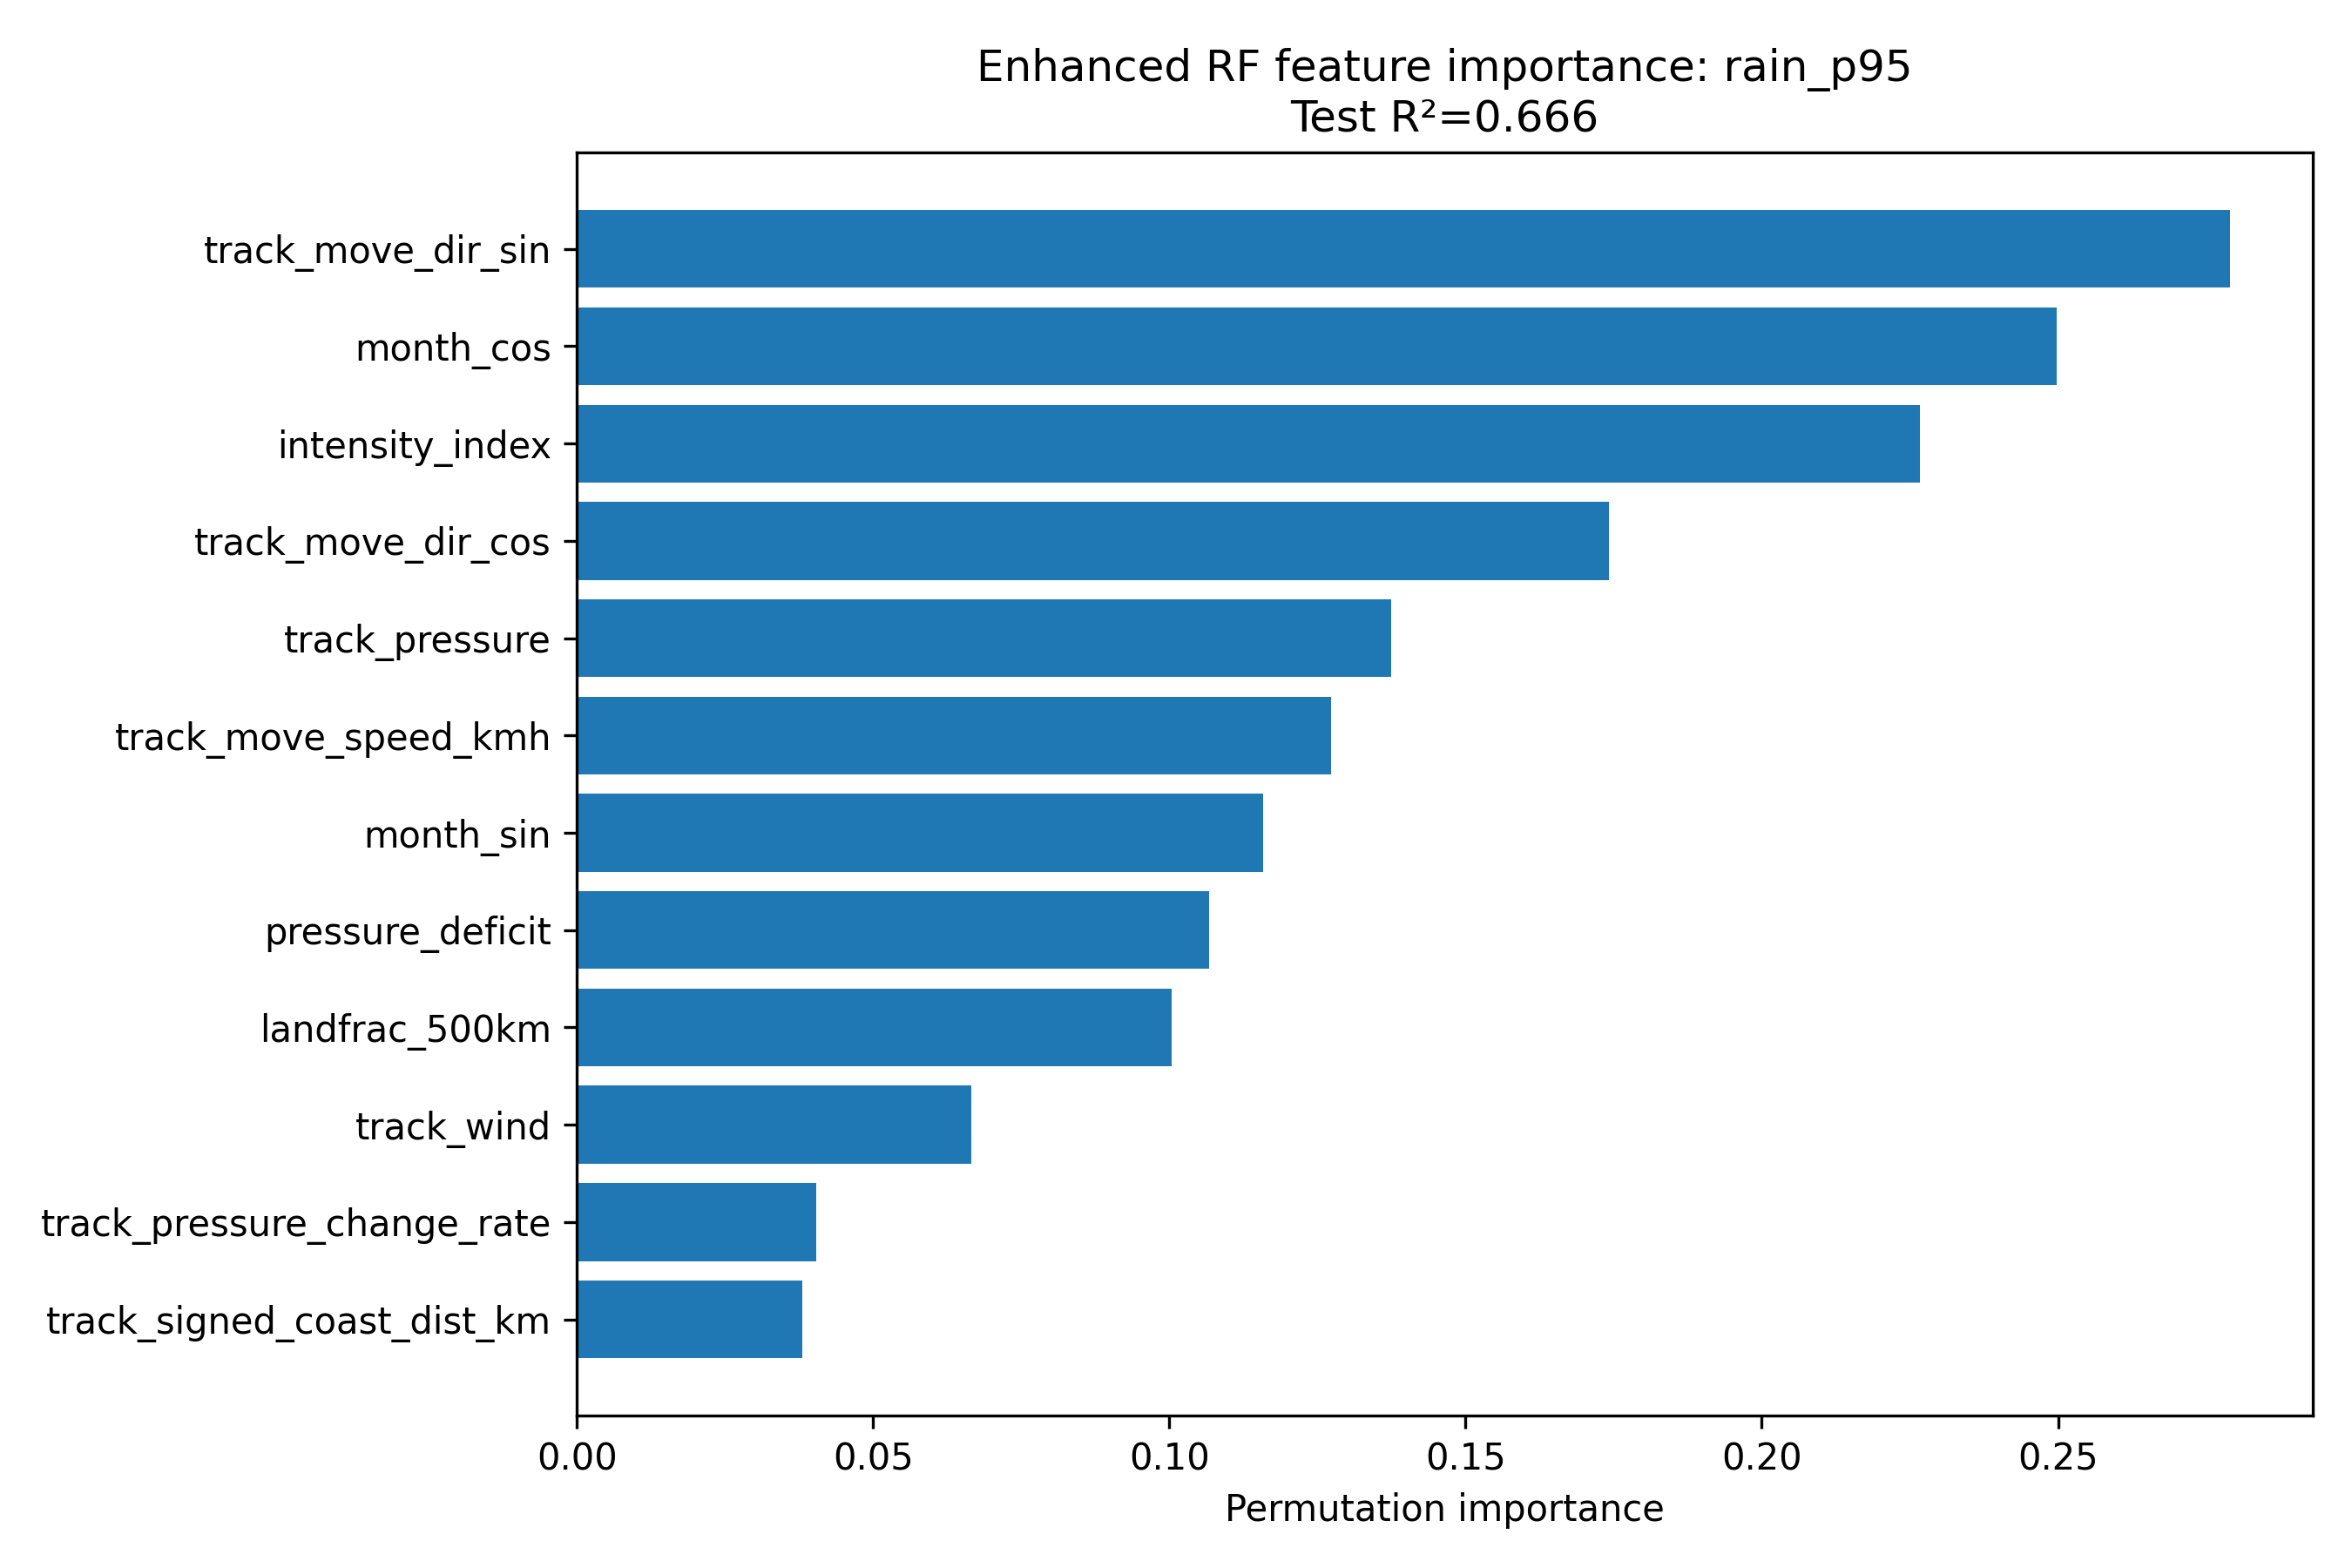
\includegraphics[width=0.78\textwidth]{outputs/figures/problem1_env/07_enhanced_rf_importance_rain_p95.png}
    \caption{补充环境变量后P95降水强度模型的随机森林特征重要性}
    \label{fig:rf_importance_p95_problem1}
\end{figure}

\begin{figure}[htbp]
    \centering
    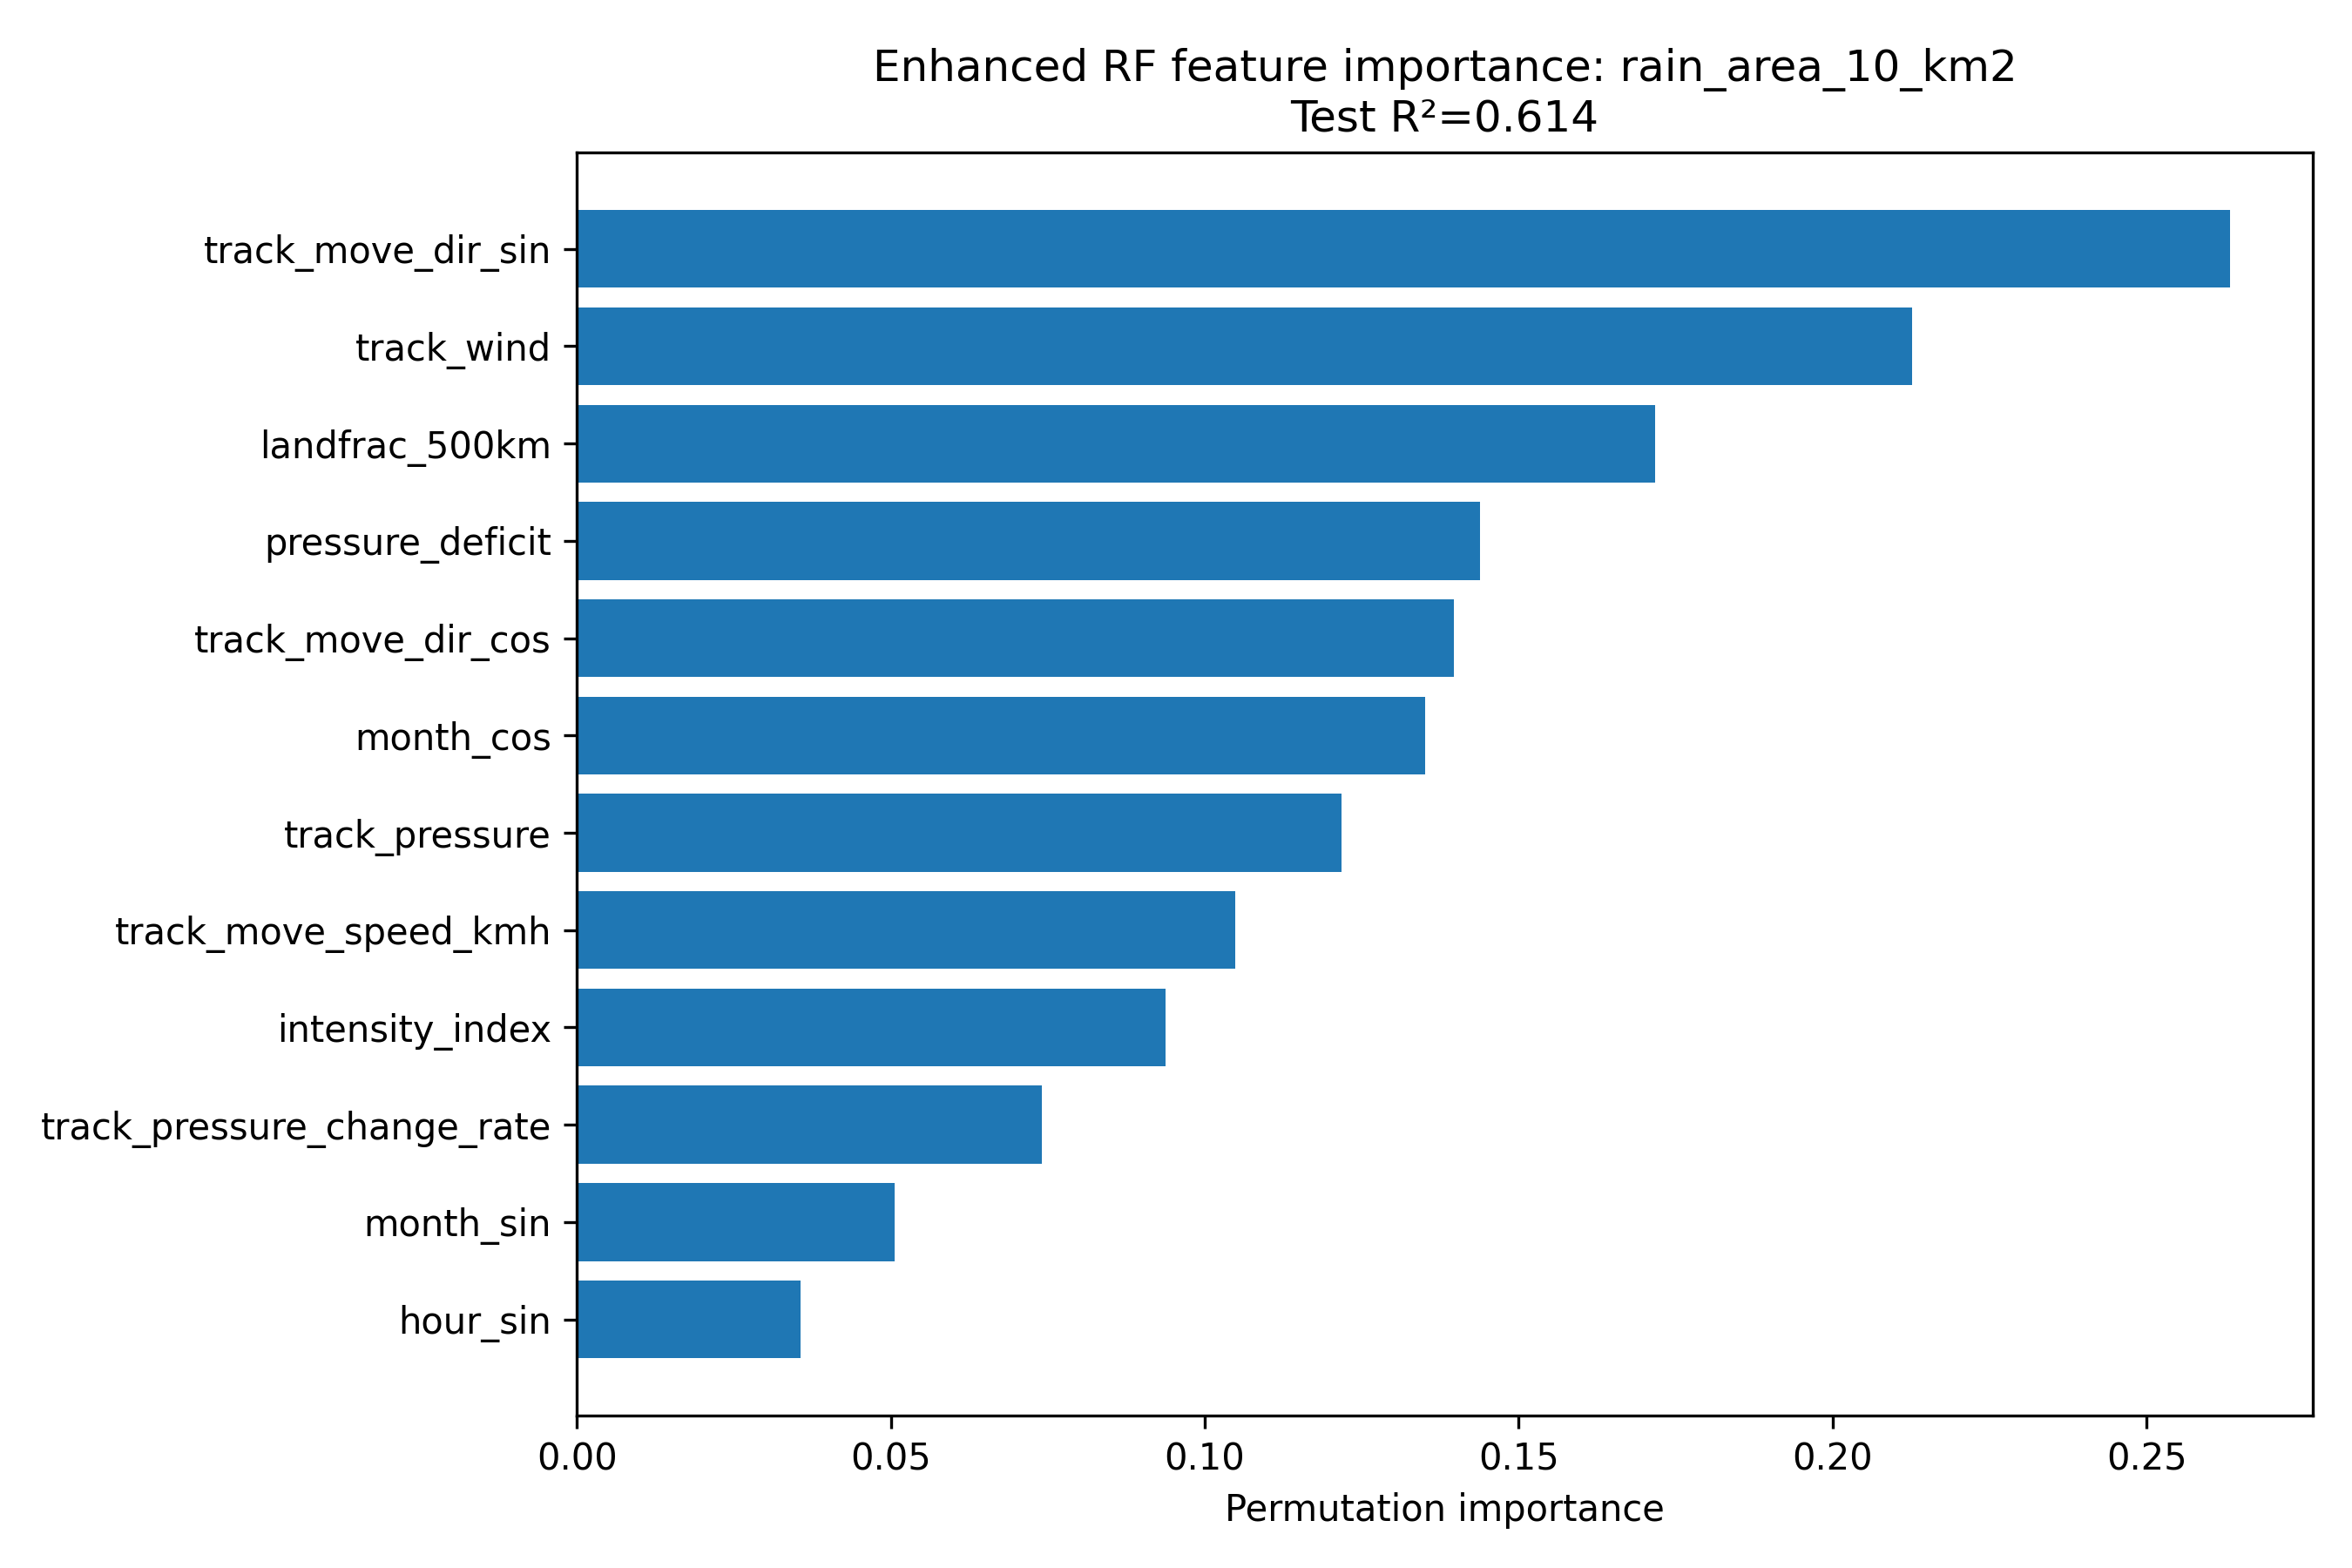
\includegraphics[width=0.78\textwidth]{outputs/figures/problem1_env/07_enhanced_rf_importance_rain_area_10_km2.png}
    \caption{补充环境变量后强降水面积模型的随机森林特征重要性}
    \label{fig:rf_importance_area10_problem1}
\end{figure}

\subsubsection{移动方向和移动速度对降水空间结构的影响}

降水质心偏移模型的测试集$R^2$为0.684，是本问题中解释效果较好的目标变量之一。随机森林结果显示，影响降水质心偏移的前五个变量依次为：移动方向正弦、移动速度、综合强度指数、月份余弦和移动方向余弦，$landfrac\_500km$ 也进入前十。说明降水中心相对于台风中心的偏移不仅与台风强度有关，也显著受到台风移动方向、移动速度和周边陆地覆盖背景影响。

图\ref{fig:move_centroid_problem1}展示了移动速度与降水质心偏移之间的关系。总体来看，移动速度越大，降水质心偏移的变化范围越大，说明台风移动过程会改变水汽输送和降水落区相对于台风中心的位置。

\begin{figure}[htbp]
    \centering
    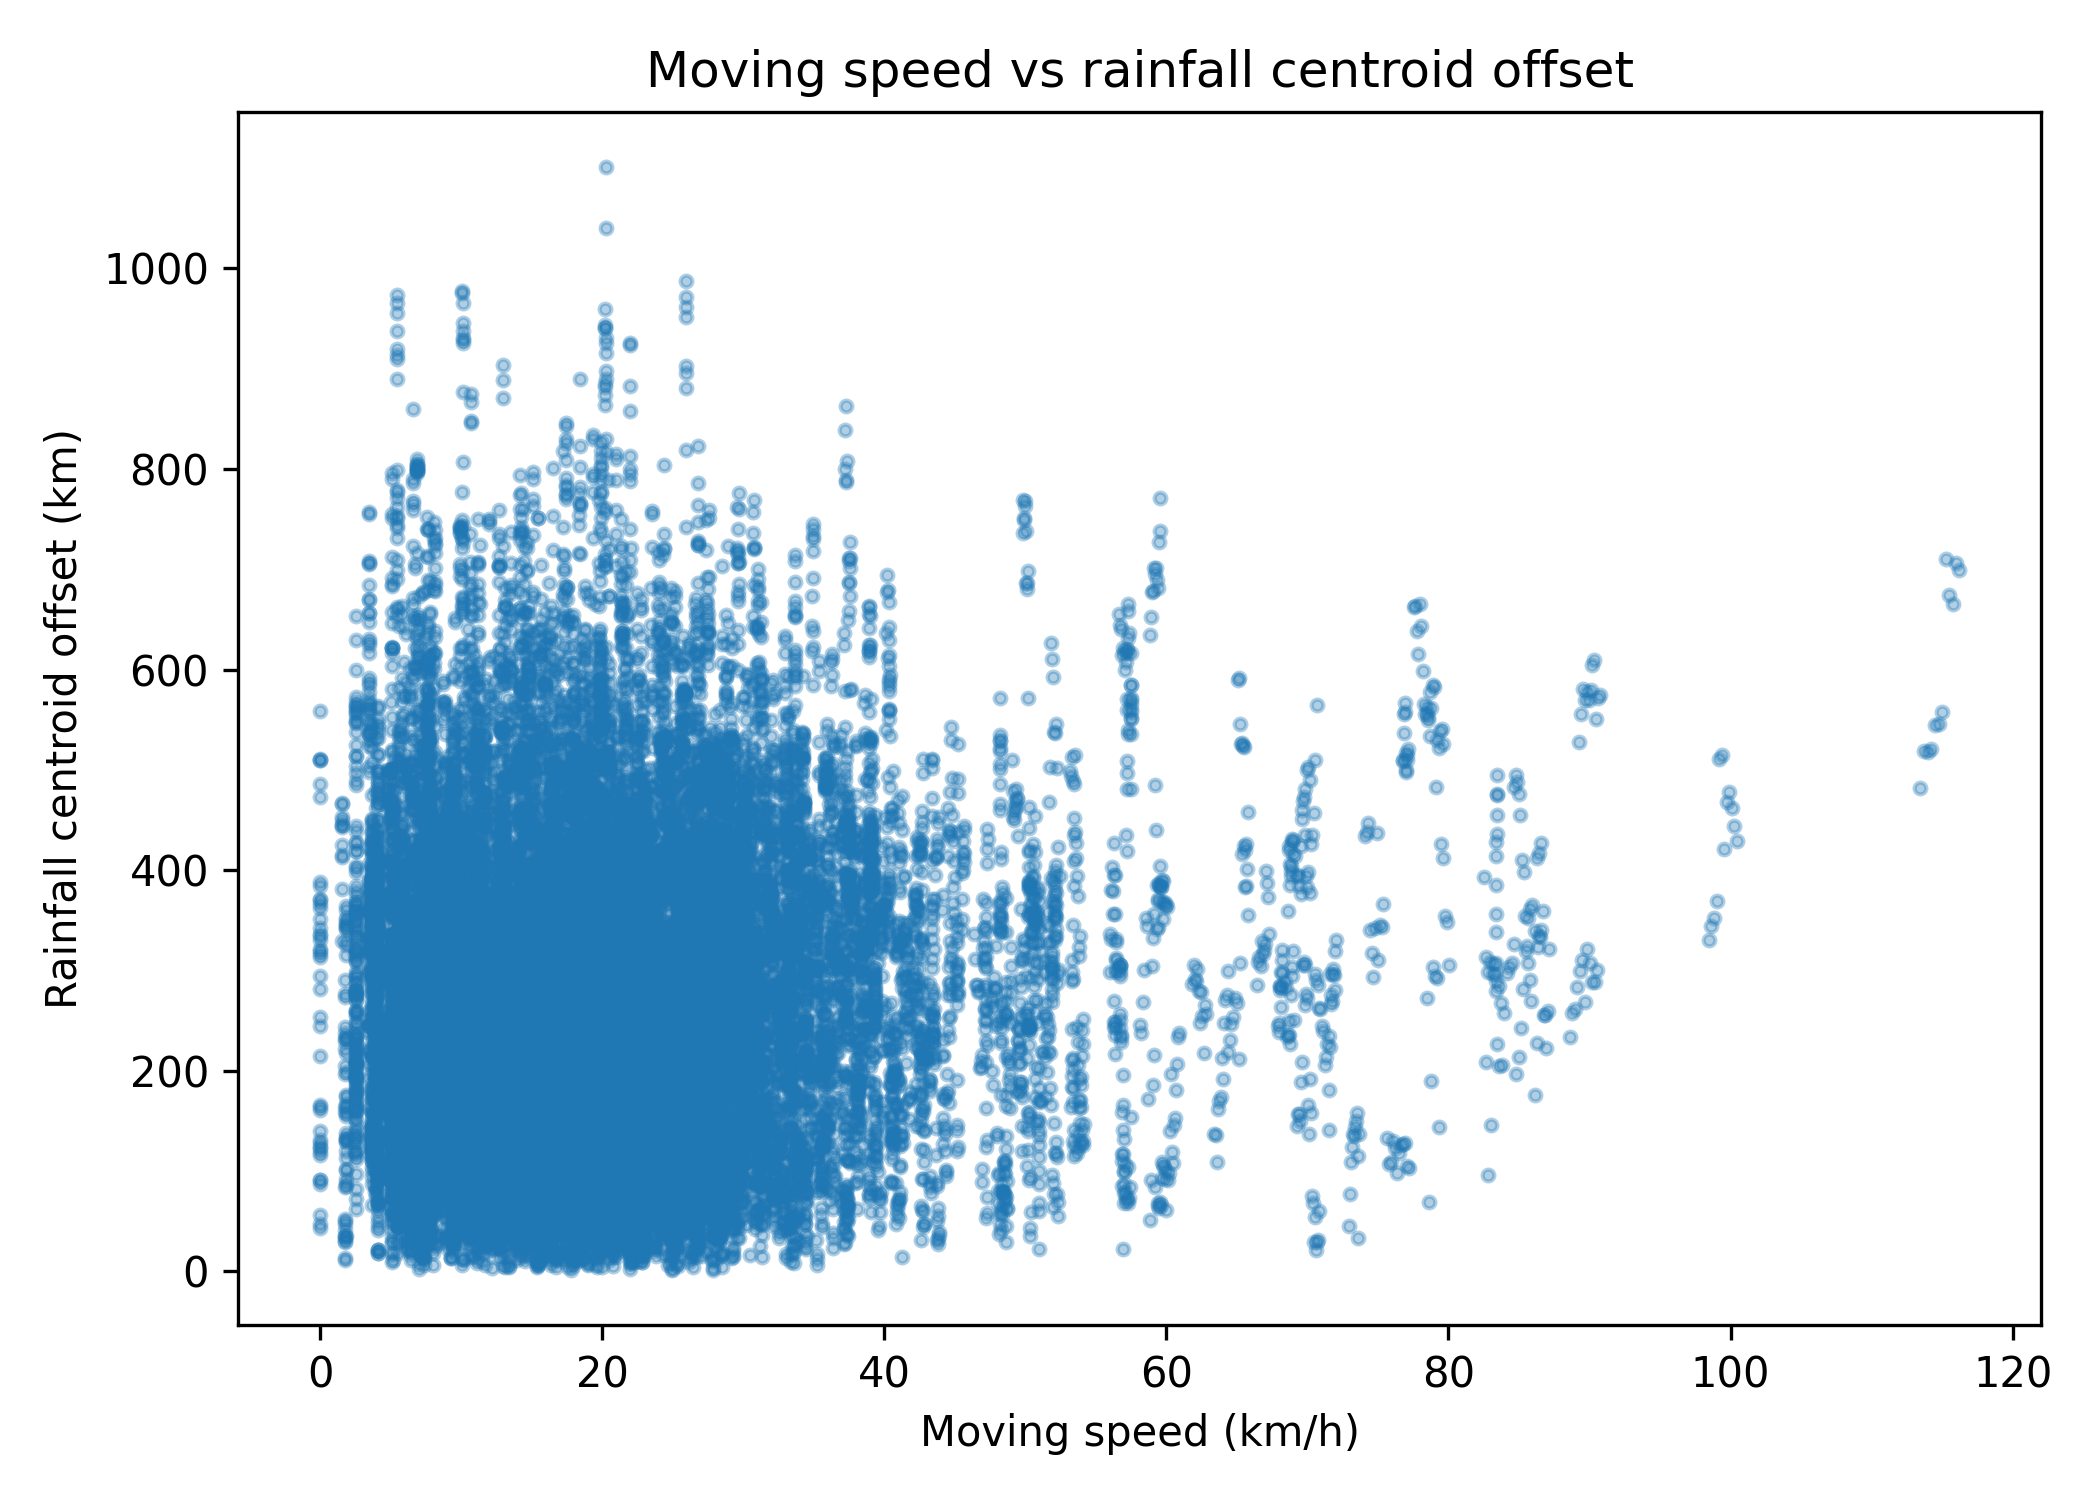
\includegraphics[width=0.72\textwidth]{outputs/figures/problem1_env/05_move_speed_vs_centroid_offset.png}
    \caption{补充环境变量后移动速度与降水质心偏移的关系}
    \label{fig:move_centroid_problem1}
\end{figure}

雨带各向异性模型的测试集$R^2$为0.640。其前五个重要变量依次为：移动方向正弦、月份余弦、移动速度、移动方向余弦和$terrain\_std\_300km$。这说明雨带是否呈狭长形态与台风行进方向、移动速度、季节背景和台风中心附近地形起伏复杂度密切相关。移动方向正弦和余弦同时进入前列，也表明用周期变量表示移动方向是必要的。

\begin{figure}[htbp]
    \centering
    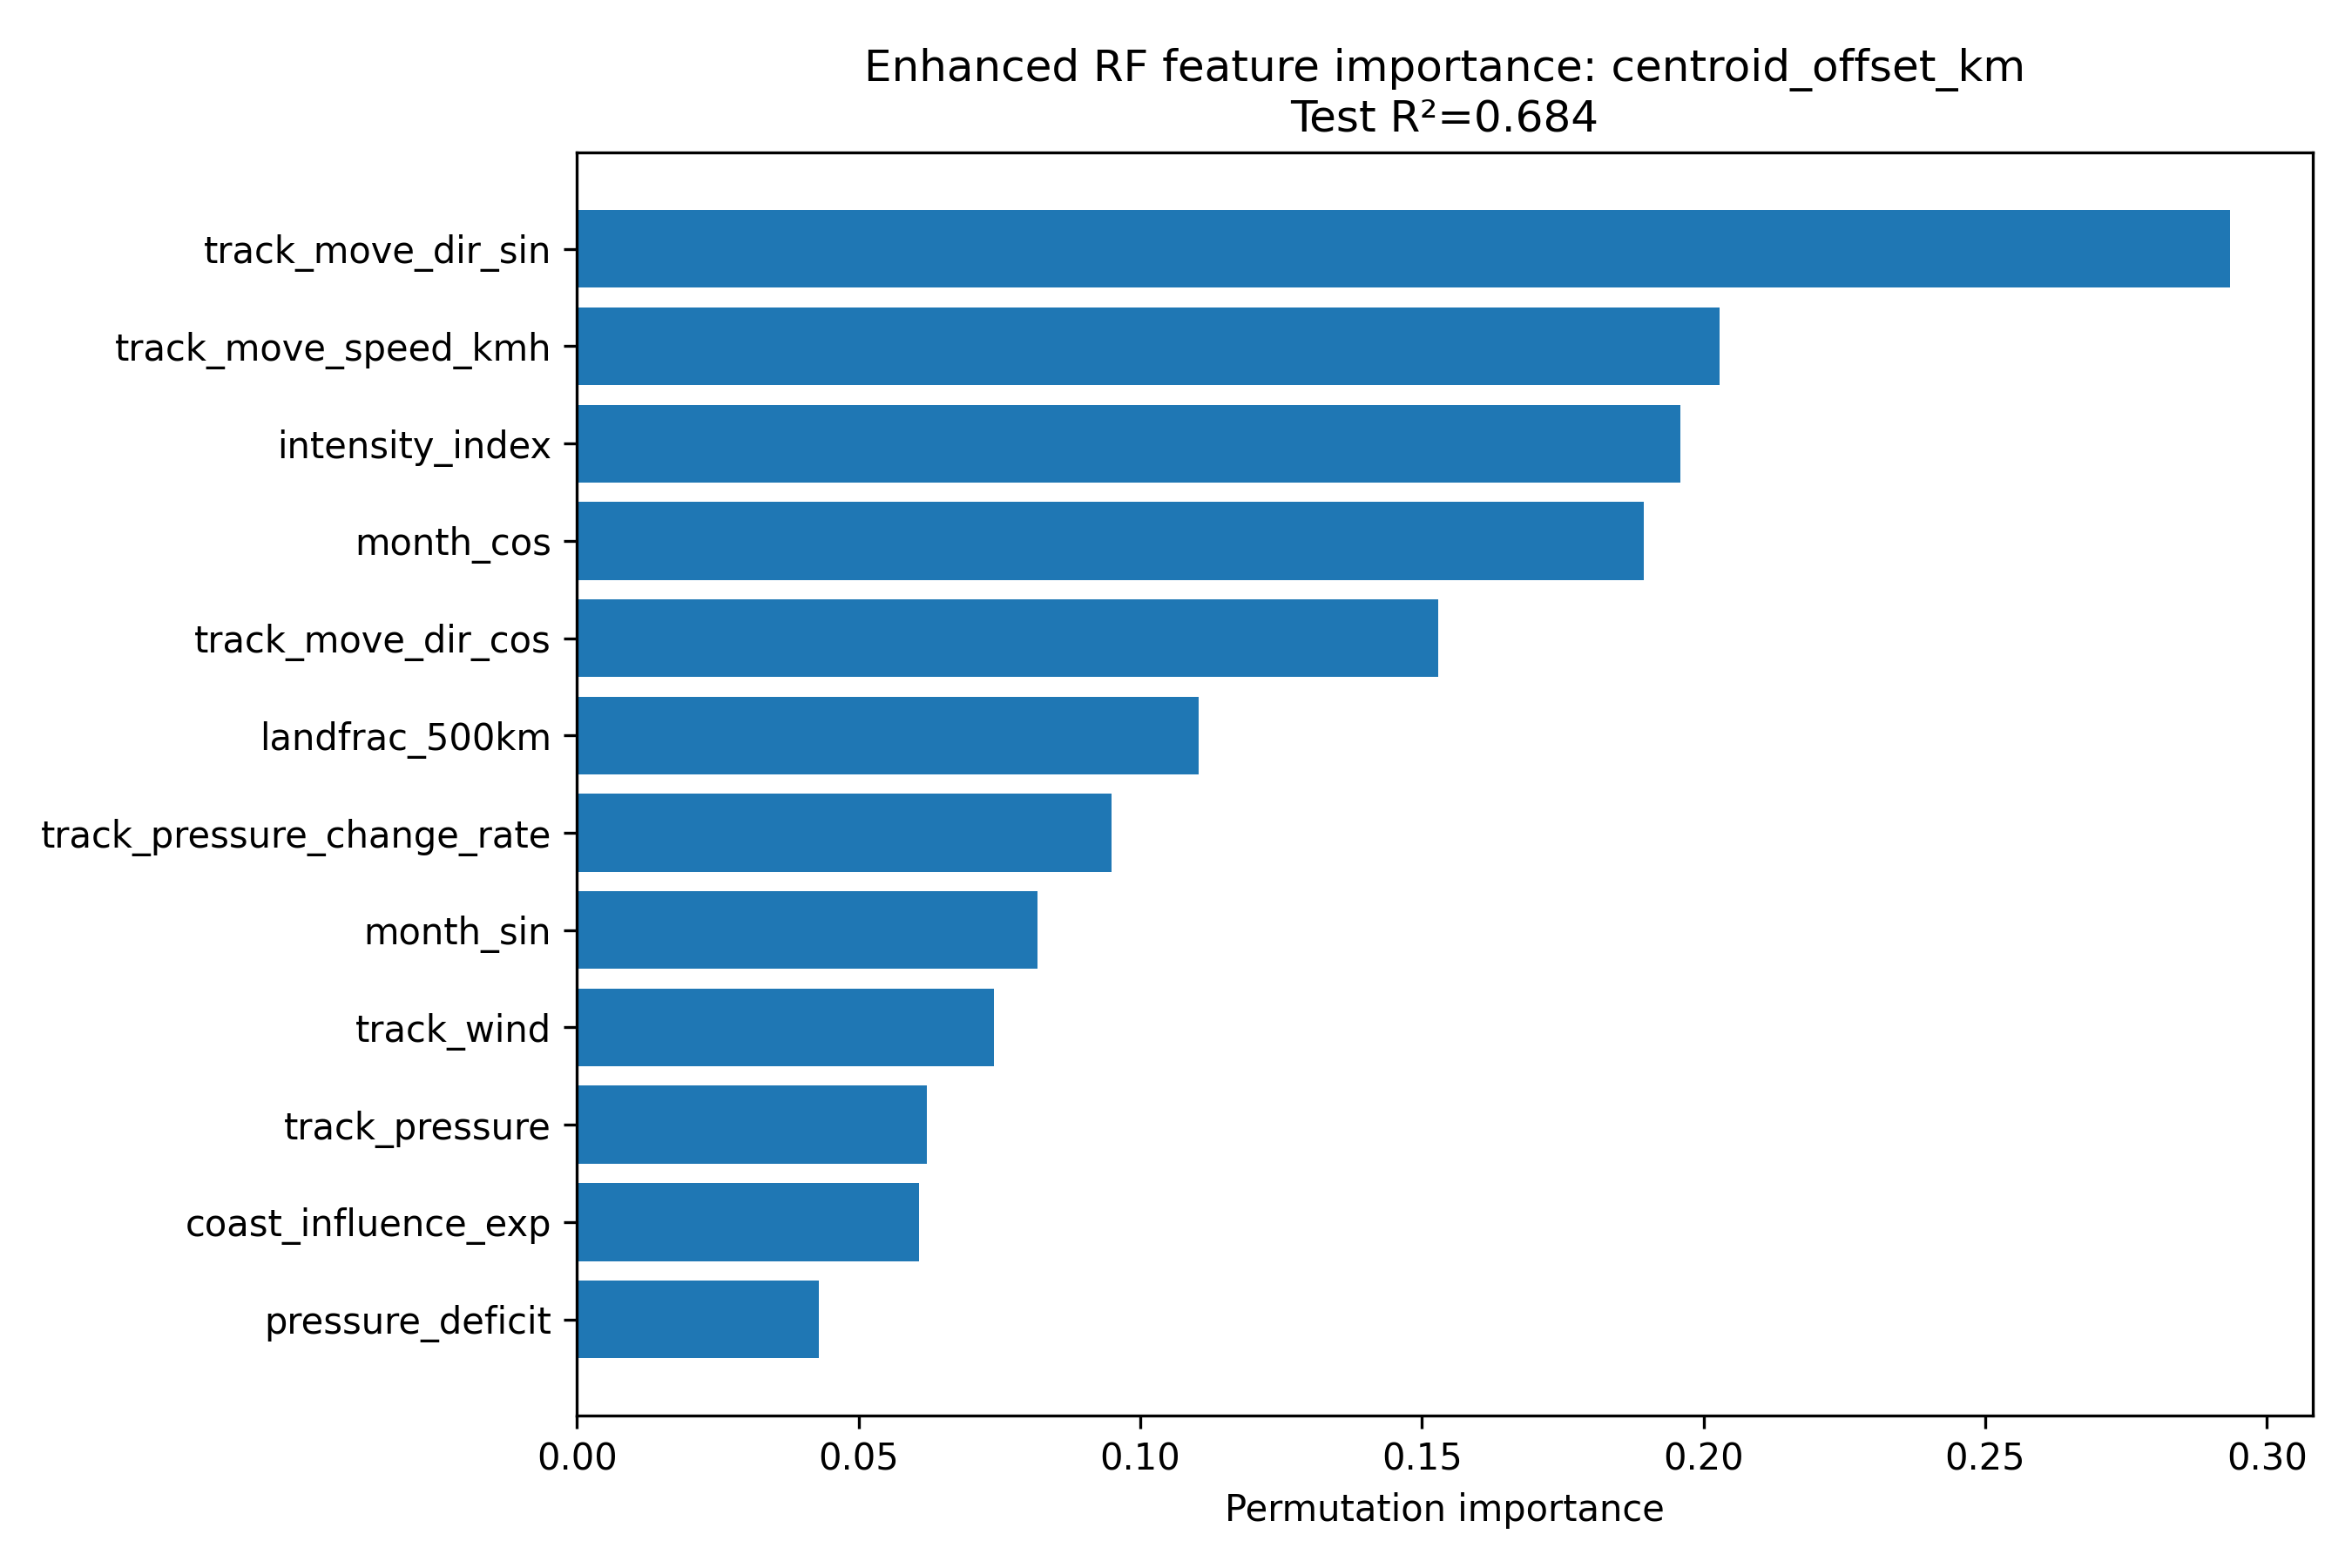
\includegraphics[width=0.78\textwidth]{outputs/figures/problem1_env/07_enhanced_rf_importance_centroid_offset_km.png}
    \caption{补充环境变量后降水质心偏移模型的随机森林特征重要性}
    \label{fig:rf_importance_centroid_problem1}
\end{figure}

\begin{figure}[htbp]
    \centering
    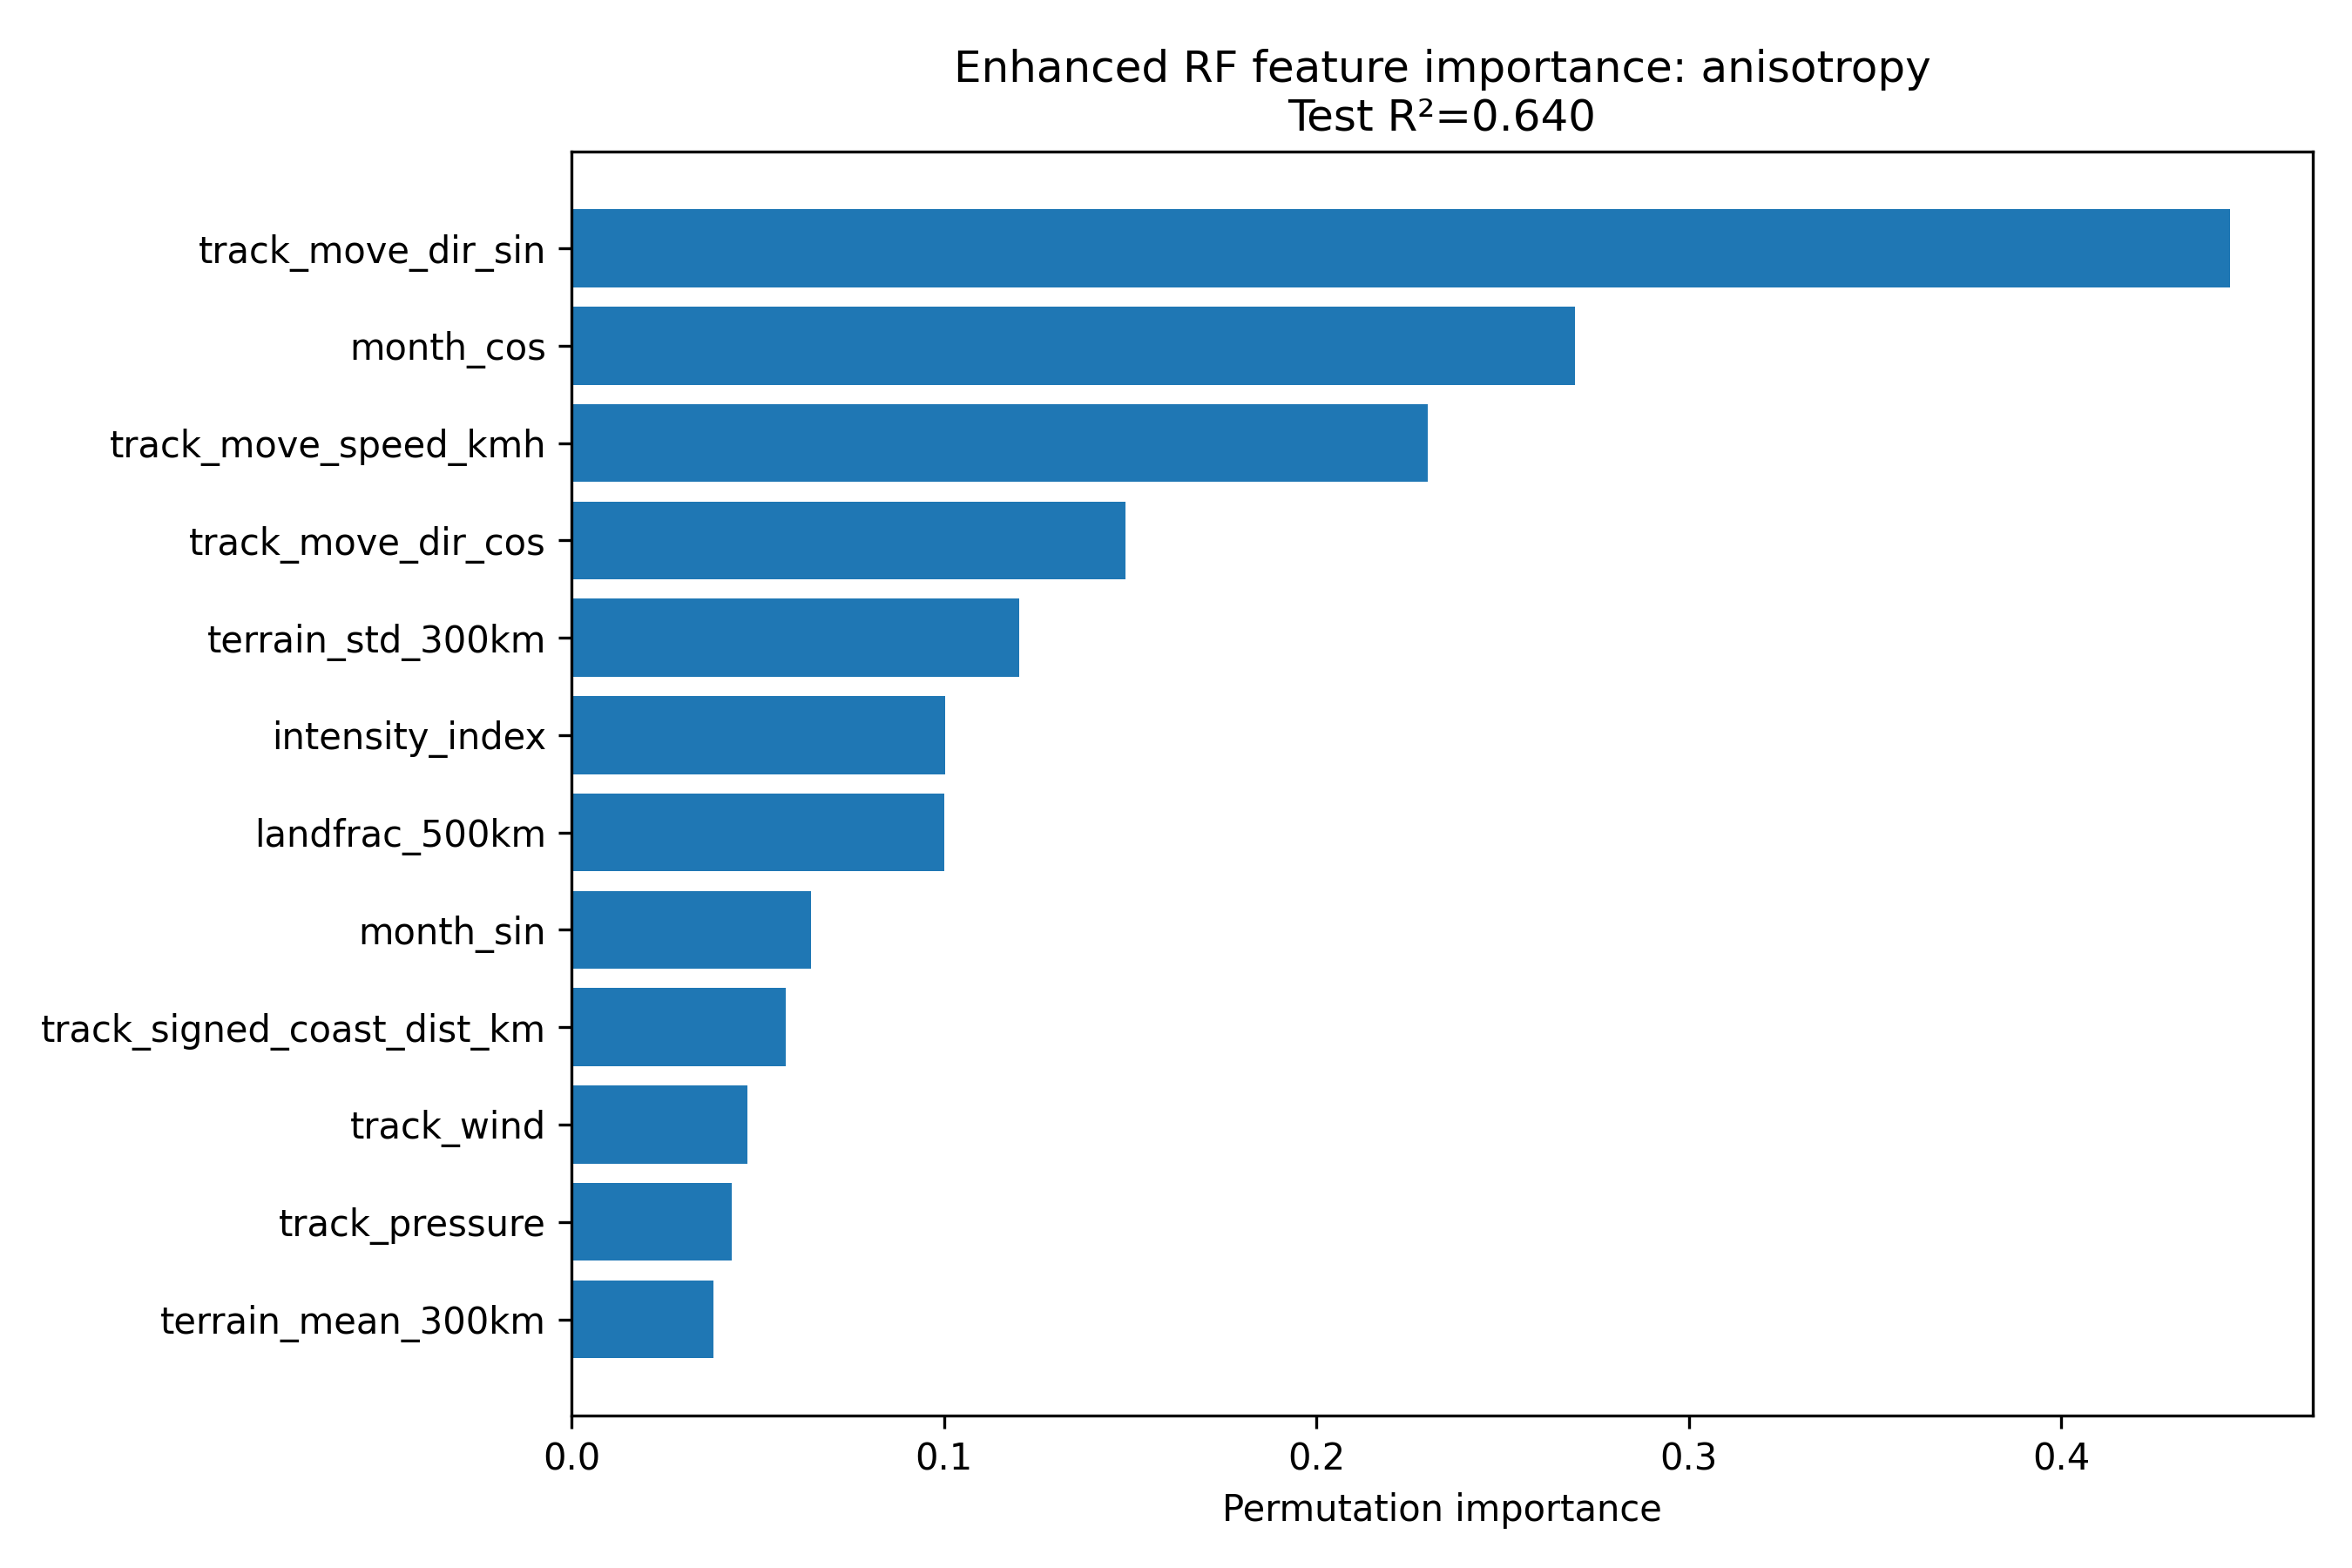
\includegraphics[width=0.78\textwidth]{outputs/figures/problem1_env/07_enhanced_rf_importance_anisotropy.png}
    \caption{补充环境变量后雨带各向异性模型的随机森林特征重要性}
    \label{fig:rf_importance_anisotropy_problem1}
\end{figure}

\subsubsection{固定地理方向下降水非对称性与台风演变的关系}

相关性结果显示，东西方向非对称性$asym\_EW$与移动方向正弦的Spearman相关系数为$0.395$，与气压变化率的相关系数为$0.184$，与风速变化率的相关系数为$-0.174$。南北方向非对称性$asym\_NS$与移动方向正弦的相关系数为$0.362$，与月份余弦的相关系数为$0.315$，与气压变化率的相关系数为$0.258$，与风速变化率的相关系数为$-0.245$。

这些结果表明，固定地理方向下的降水非对称性不是单纯由当前风速或中心气压决定，而与台风移动方向、增强或减弱过程以及季节背景共同相关。换言之，台风降水空间偏向不仅反映台风当前强度，也反映台风演变状态和背景环流条件。

图\ref{fig:centroid_motion_hist_problem1}展示了降水质心方向相对于台风移动方向的分布，用于辅助说明降水偏移与台风运动方向之间的联系。

\begin{figure}[htbp]
    \centering
    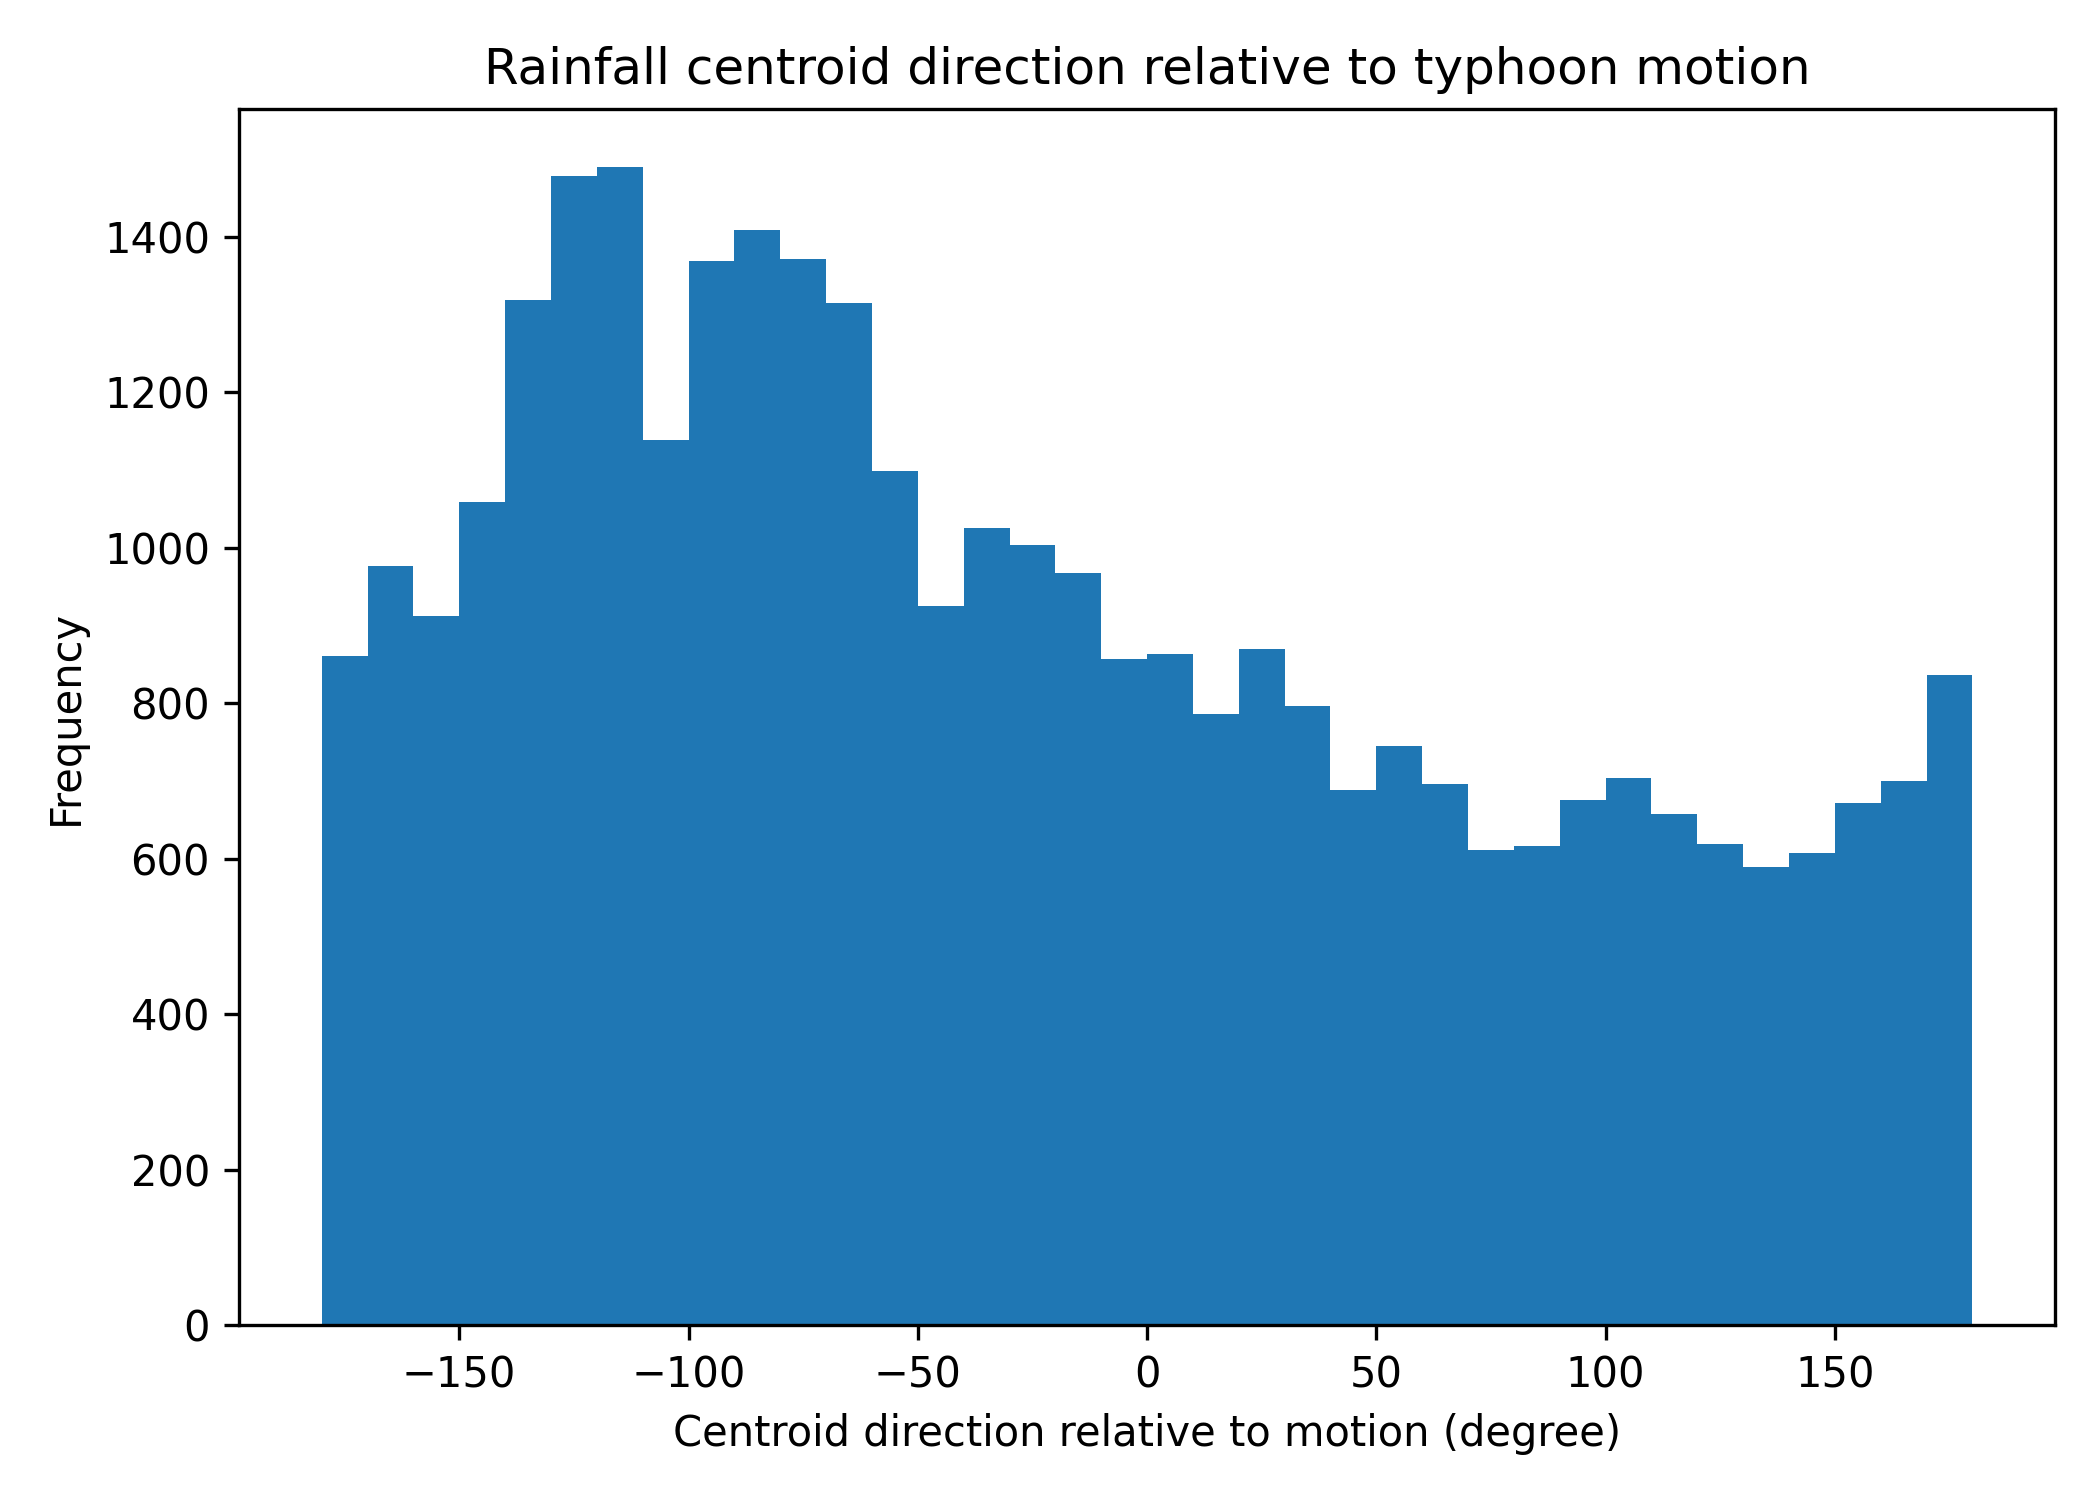
\includegraphics[width=0.72\textwidth]{outputs/figures/problem1_interp/06_centroid_relative_to_motion_hist.png}
    \caption{降水质心方向相对于台风移动方向的分布}
    \label{fig:centroid_motion_hist_problem1}
\end{figure}

\subsubsection{台风相对运动坐标系下的降水偏向特征}

为进一步检验降水分布是否相对于台风移动方向存在系统性偏向，本文基于逐格旋转后的台风相对运动坐标系，统计了前后、左右及四象限降水比例。结果显示，历史样本中降水整体更偏向台风移动前方和左侧。所有有效样本中，前方降水比例均值为$54.1\%$，后方为$45.9\%$；左侧降水比例均值为$55.0\%$，右侧为$45.0\%$。对应地，前后非对称性$A_{FB}$的均值和中位数分别为$0.083$和$0.056$，左右非对称性$A_{LR}$的均值和中位数分别为$0.100$和$0.138$。

\begin{figure}[htbp]
    \centering
    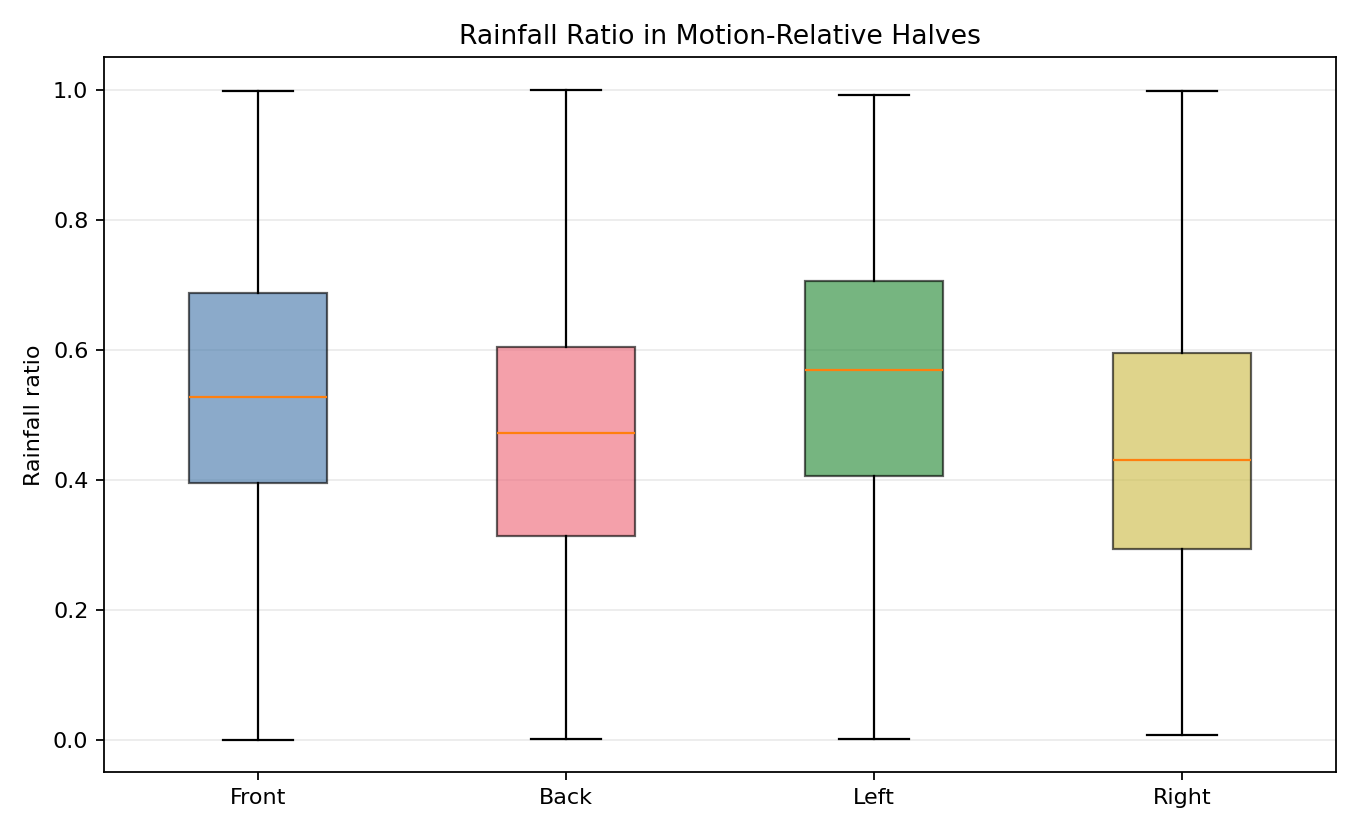
\includegraphics[width=0.78\textwidth]{outputs/figures/problem1_motion/01_motion_half_ratio_boxplot.png}
    \caption{台风相对运动坐标系下前后、左右降水比例分布}
    \label{fig:motion_fb_lr_ratio_problem1}
\end{figure}

进一步考察四象限降水比例可发现，平均和中位数最大的均为前左象限。四象限平均比例分别为：前左象限$30.2\%$、前右象限$24.0\%$、后左象限$24.8\%$、后右象限$21.0\%$。这说明台风降水并不是在台风中心周围均匀分布，而是相对于移动方向存在明显的前侧和左侧偏向。

\begin{figure}[htbp]
    \centering
    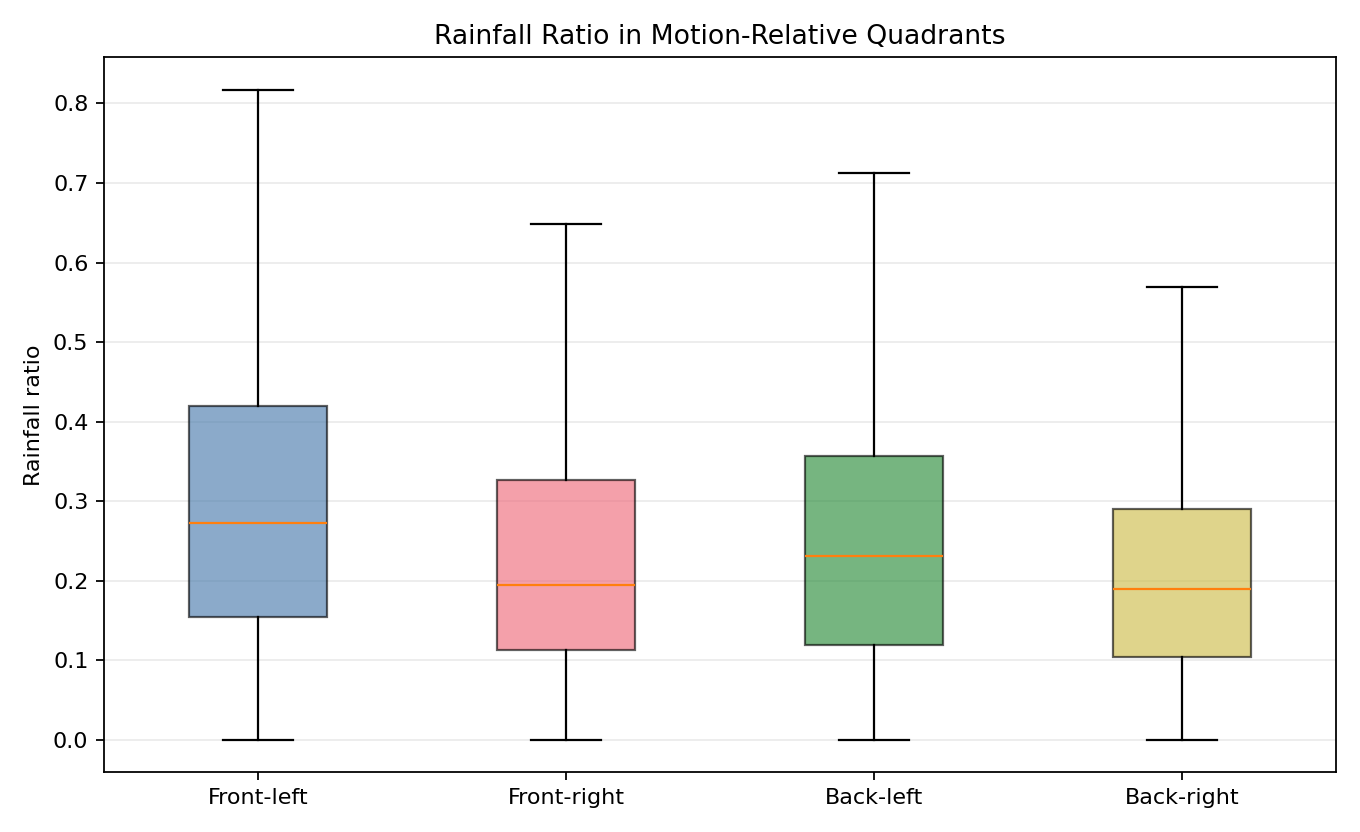
\includegraphics[width=0.78\textwidth]{outputs/figures/problem1_motion/02_motion_quadrant_ratio_boxplot.png}
    \caption{台风相对运动坐标系下四象限降水比例分布}
    \label{fig:motion_quadrant_ratio_problem1}
\end{figure}

从强降水面积看，$10\ \mathrm{mm/hr}$以上强降水面积在台风前方和左侧也更大。其中，前方强降水面积中位数为$17158.9\ \mathrm{km^2}$，后方为$11962.6\ \mathrm{km^2}$；左侧强降水面积中位数为$17761.9\ \mathrm{km^2}$，右侧为$11591.7\ \mathrm{km^2}$。这进一步表明，台风运动方向不仅影响降水总量分布，也会影响强降水区域的位置。

\begin{figure}[htbp]
    \centering
    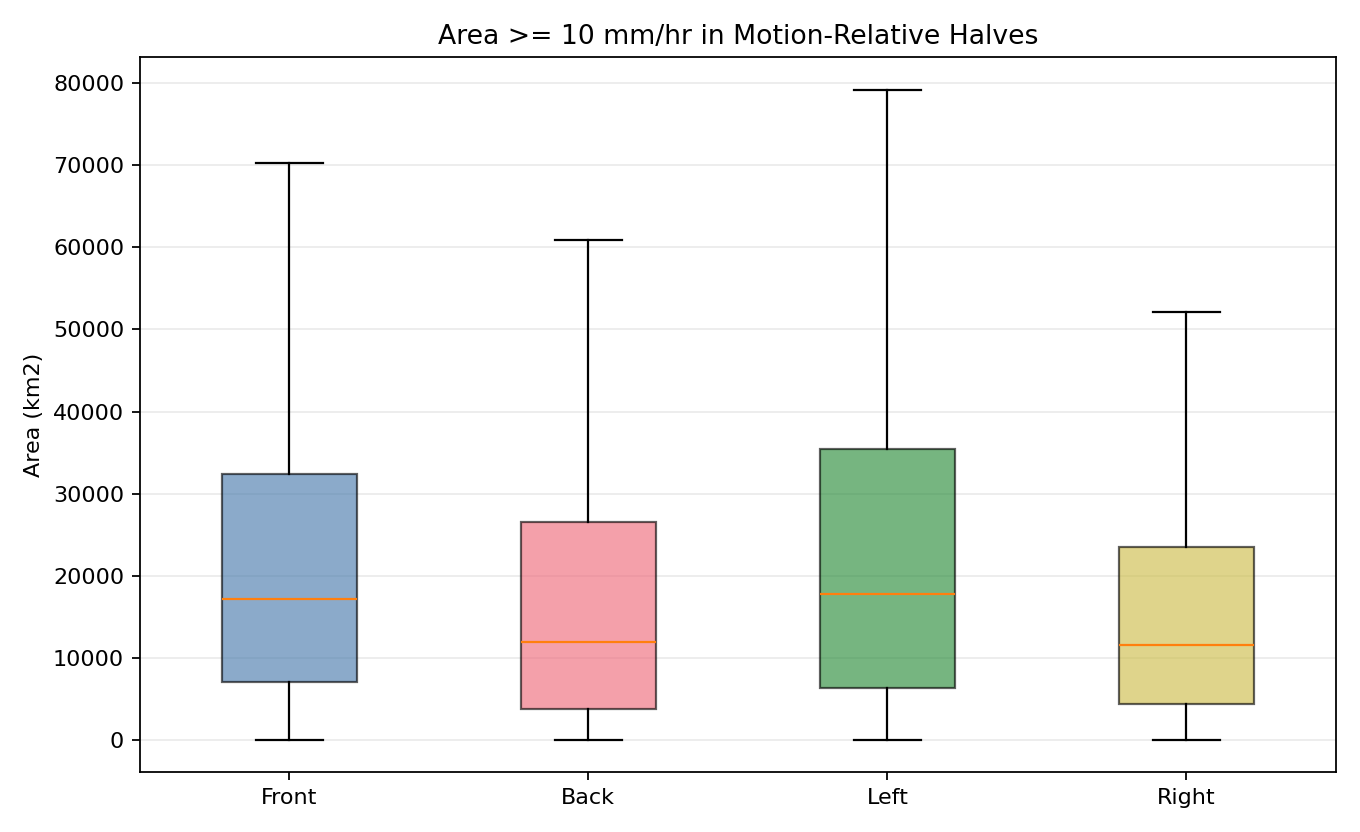
\includegraphics[width=0.78\textwidth]{outputs/figures/problem1_motion/05_motion_area10_boxplot.png}
    \caption{台风相对运动坐标系下$10\ \mathrm{mm/hr}$以上强降水面积分布}
    \label{fig:motion_area10_problem1}
\end{figure}

此外，雨带主轴相对于台风移动方向的夹角均值和中位数分别约为$44.9^\circ$和$44.8^\circ$，说明降水带通常并非严格沿台风移动方向伸展，而是与移动方向存在一定斜交角。这一结果表明，雨带结构受到台风移动方向、环境风场和水汽输送方向共同调制。

\begin{figure}[htbp]
    \centering
    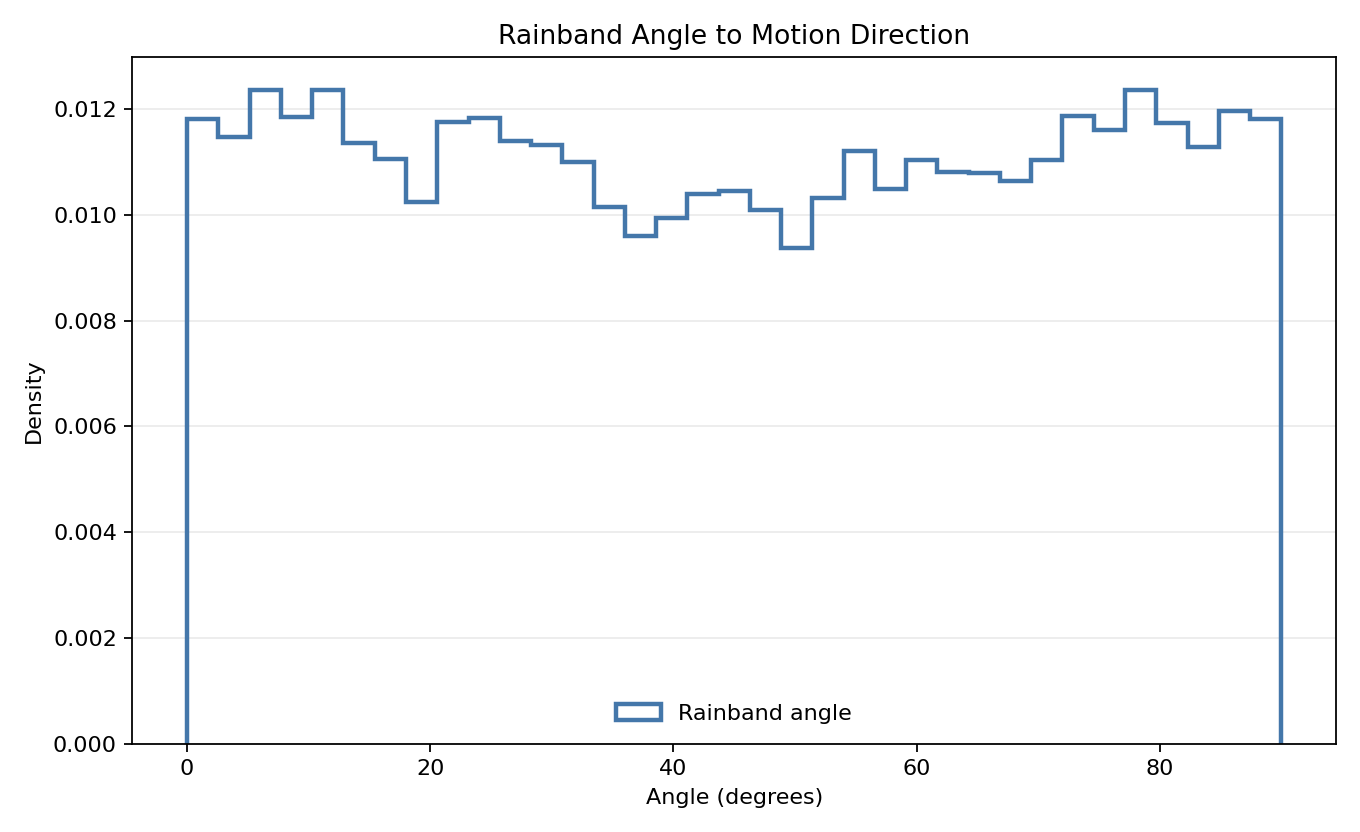
\includegraphics[width=0.72\textwidth]{outputs/figures/problem1_motion/04_rainband_angle_to_motion_hist.png}
    \caption{雨带主轴相对于台风移动方向的夹角分布}
    \label{fig:rainband_motion_angle_problem1}
\end{figure}

表\ref{tab:motion_relative_stats_problem1}汇总了台风相对运动坐标系下的主要降水结构指标。

\begin{table}[htbp]
    \centering
    \caption{台风相对运动坐标系下降水结构指标统计}
    \label{tab:motion_relative_stats_problem1}
    \begin{tabular}{lcc}
        \hline
        指标 & 均值 & 中位数 \\
        \hline
        前方降水比例 & 0.541 & -- \\
        后方降水比例 & 0.459 & -- \\
        左侧降水比例 & 0.550 & -- \\
        右侧降水比例 & 0.450 & -- \\
        前后非对称性$A_{FB}$ & 0.083 & 0.056 \\
        左右非对称性$A_{LR}$ & 0.100 & 0.138 \\
        前左象限比例 & 0.302 & -- \\
        前右象限比例 & 0.240 & -- \\
        后左象限比例 & 0.248 & -- \\
        后右象限比例 & 0.210 & -- \\
        雨带相对运动方向夹角 & $44.9^\circ$ & $44.8^\circ$ \\
        雨带横向等效带宽$B$ / km & 1149.4 & 1118.0 \\
        雨带主轴等效长度$L$ / km & 1978.8 & 1952.7 \\
        \hline
    \end{tabular}
\end{table}

\subsubsection{降水带宽的影响因素分析}

按上述协方差定义计算后，历史样本中主雨带横向等效带宽 $B$ 的有效样本数为33310，均值为 $1149.4\ \mathrm{km}$，中位数为 $1118.0\ \mathrm{km}$；对应主轴等效长度 $L$ 的均值和中位数分别为 $1978.8\ \mathrm{km}$ 和 $1952.7\ \mathrm{km}$。强降水格点（$R\geq10\ \mathrm{mm/hr}$）上的带宽 $B_{10}$ 有效样本数为32568，均值为 $675.6\ \mathrm{km}$，中位数为 $602.1\ \mathrm{km}$，说明极端雨带通常比总体雨带更集中。

以 $rainband\_width\_km$ 为响应变量建立增强随机森林模型，普通随机划分测试集 $R^2=0.708$，MAE 为 $154.8\ \mathrm{km}$，RMSE 为 $200.4\ \mathrm{km}$。置换重要性前五变量依次为移动方向正弦、月份余弦、移动速度、500 km 陆地覆盖比例和最大风速，说明雨带横向扩展不仅受路径方向和移动速度控制，也受季节背景、海陆分布和台风强度共同调制。移动较快或方向差异明显时，降水带相对于移动方向的组织方式更容易改变；较大的陆地覆盖和复杂下垫面条件会通过摩擦、地形抬升和水汽供应差异影响雨带横向铺展；强度变量则主要反映台风环流能够维持的降水组织尺度。

需要注意的是，按台风事件分组验证后，$rainband\_width\_km$ 的测试集 $R^2$ 降至 $-0.015$，20次重复分组验证的平均 $R^2$ 约为 $-0.011$。这表明该模型适合解释历史样本内部的带宽变化关系，但不能直接作为未知台风的逐时带宽外推模型。因此，在问题二和问题三中，降水带宽仅作为生成结果的诊断指标输出，不作为目标台风生成的安全输入变量。

\begin{figure}[htbp]
    \centering
    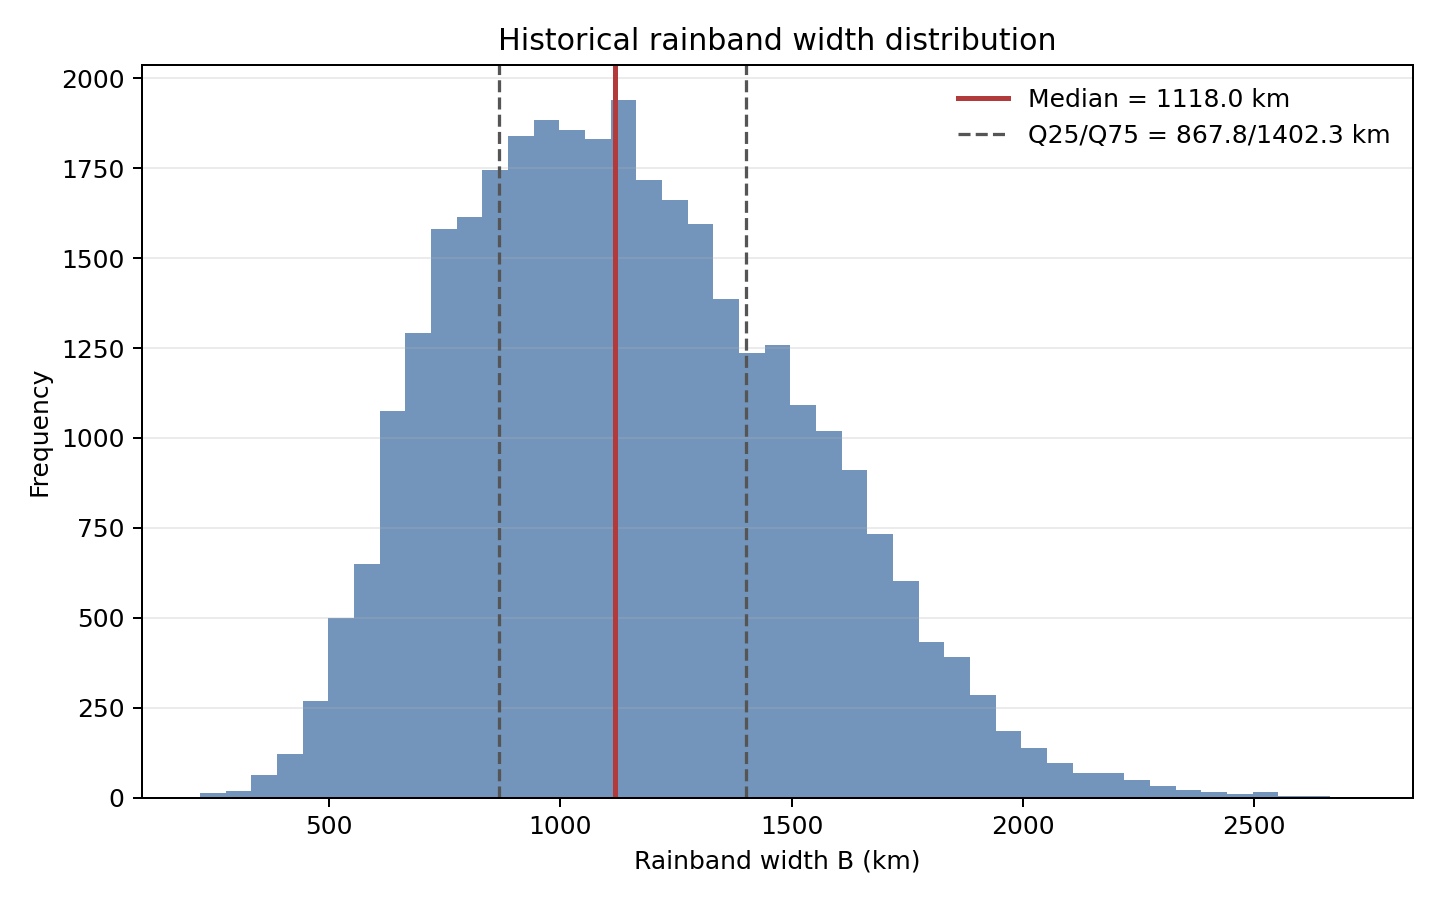
\includegraphics[width=0.72\textwidth]{outputs/figures/problem1_env/rainband_width_distribution.png}
    \caption{历史样本雨带横向等效带宽分布}
    \label{fig:rainband_width_distribution}
\end{figure}

\begin{figure}[htbp]
    \centering
    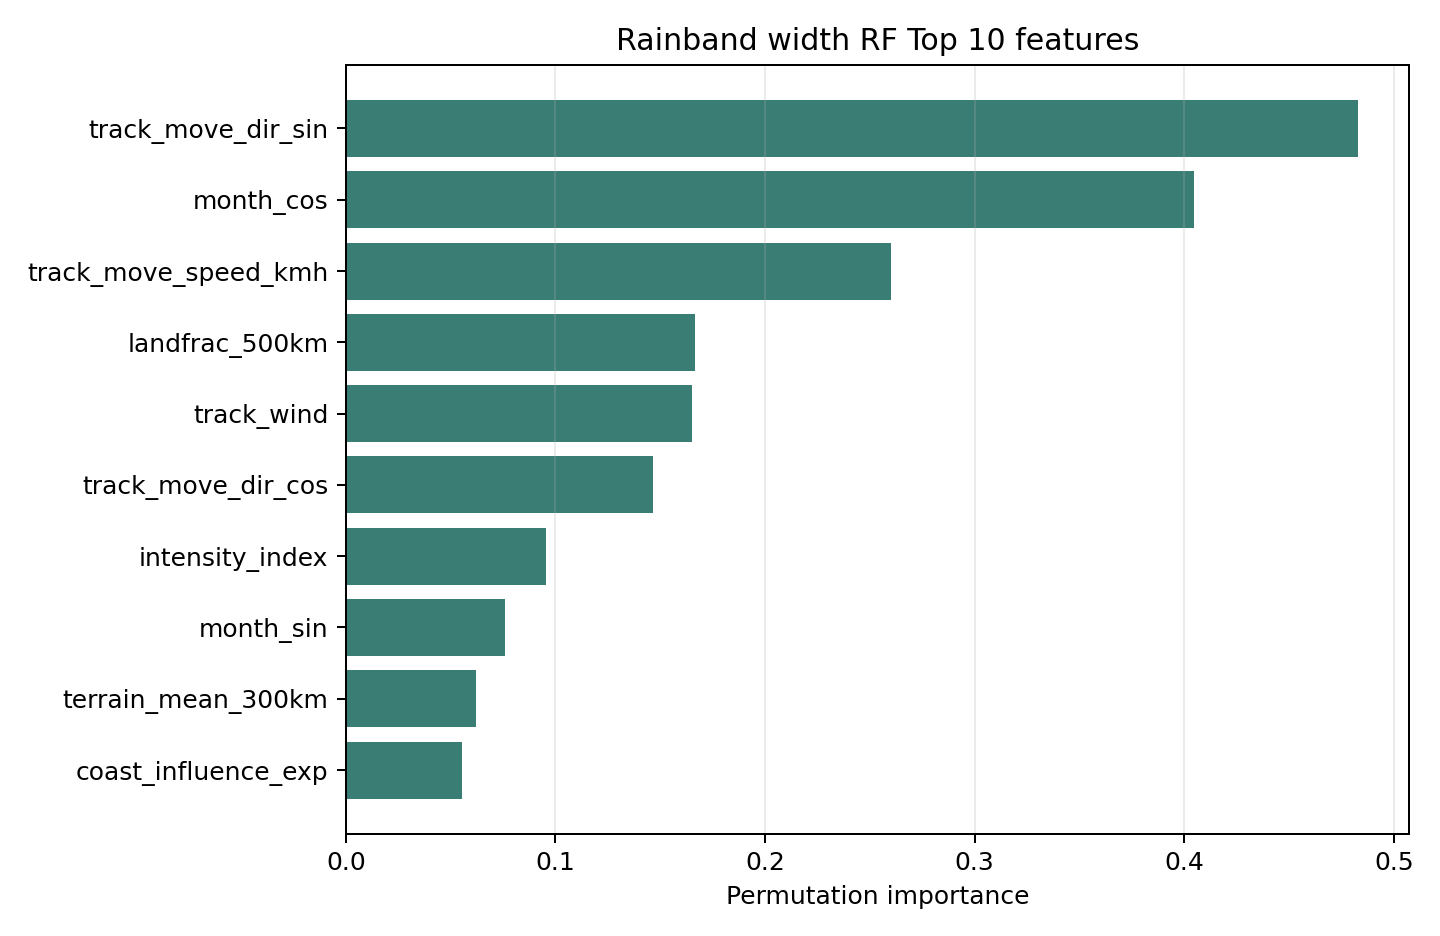
\includegraphics[width=0.82\textwidth]{outputs/figures/problem1_env/rainband_width_feature_importance.png}
    \caption{雨带横向等效带宽随机森林重要变量}
    \label{fig:rainband_width_feature_importance}
\end{figure}

\begin{figure}[htbp]
    \centering
    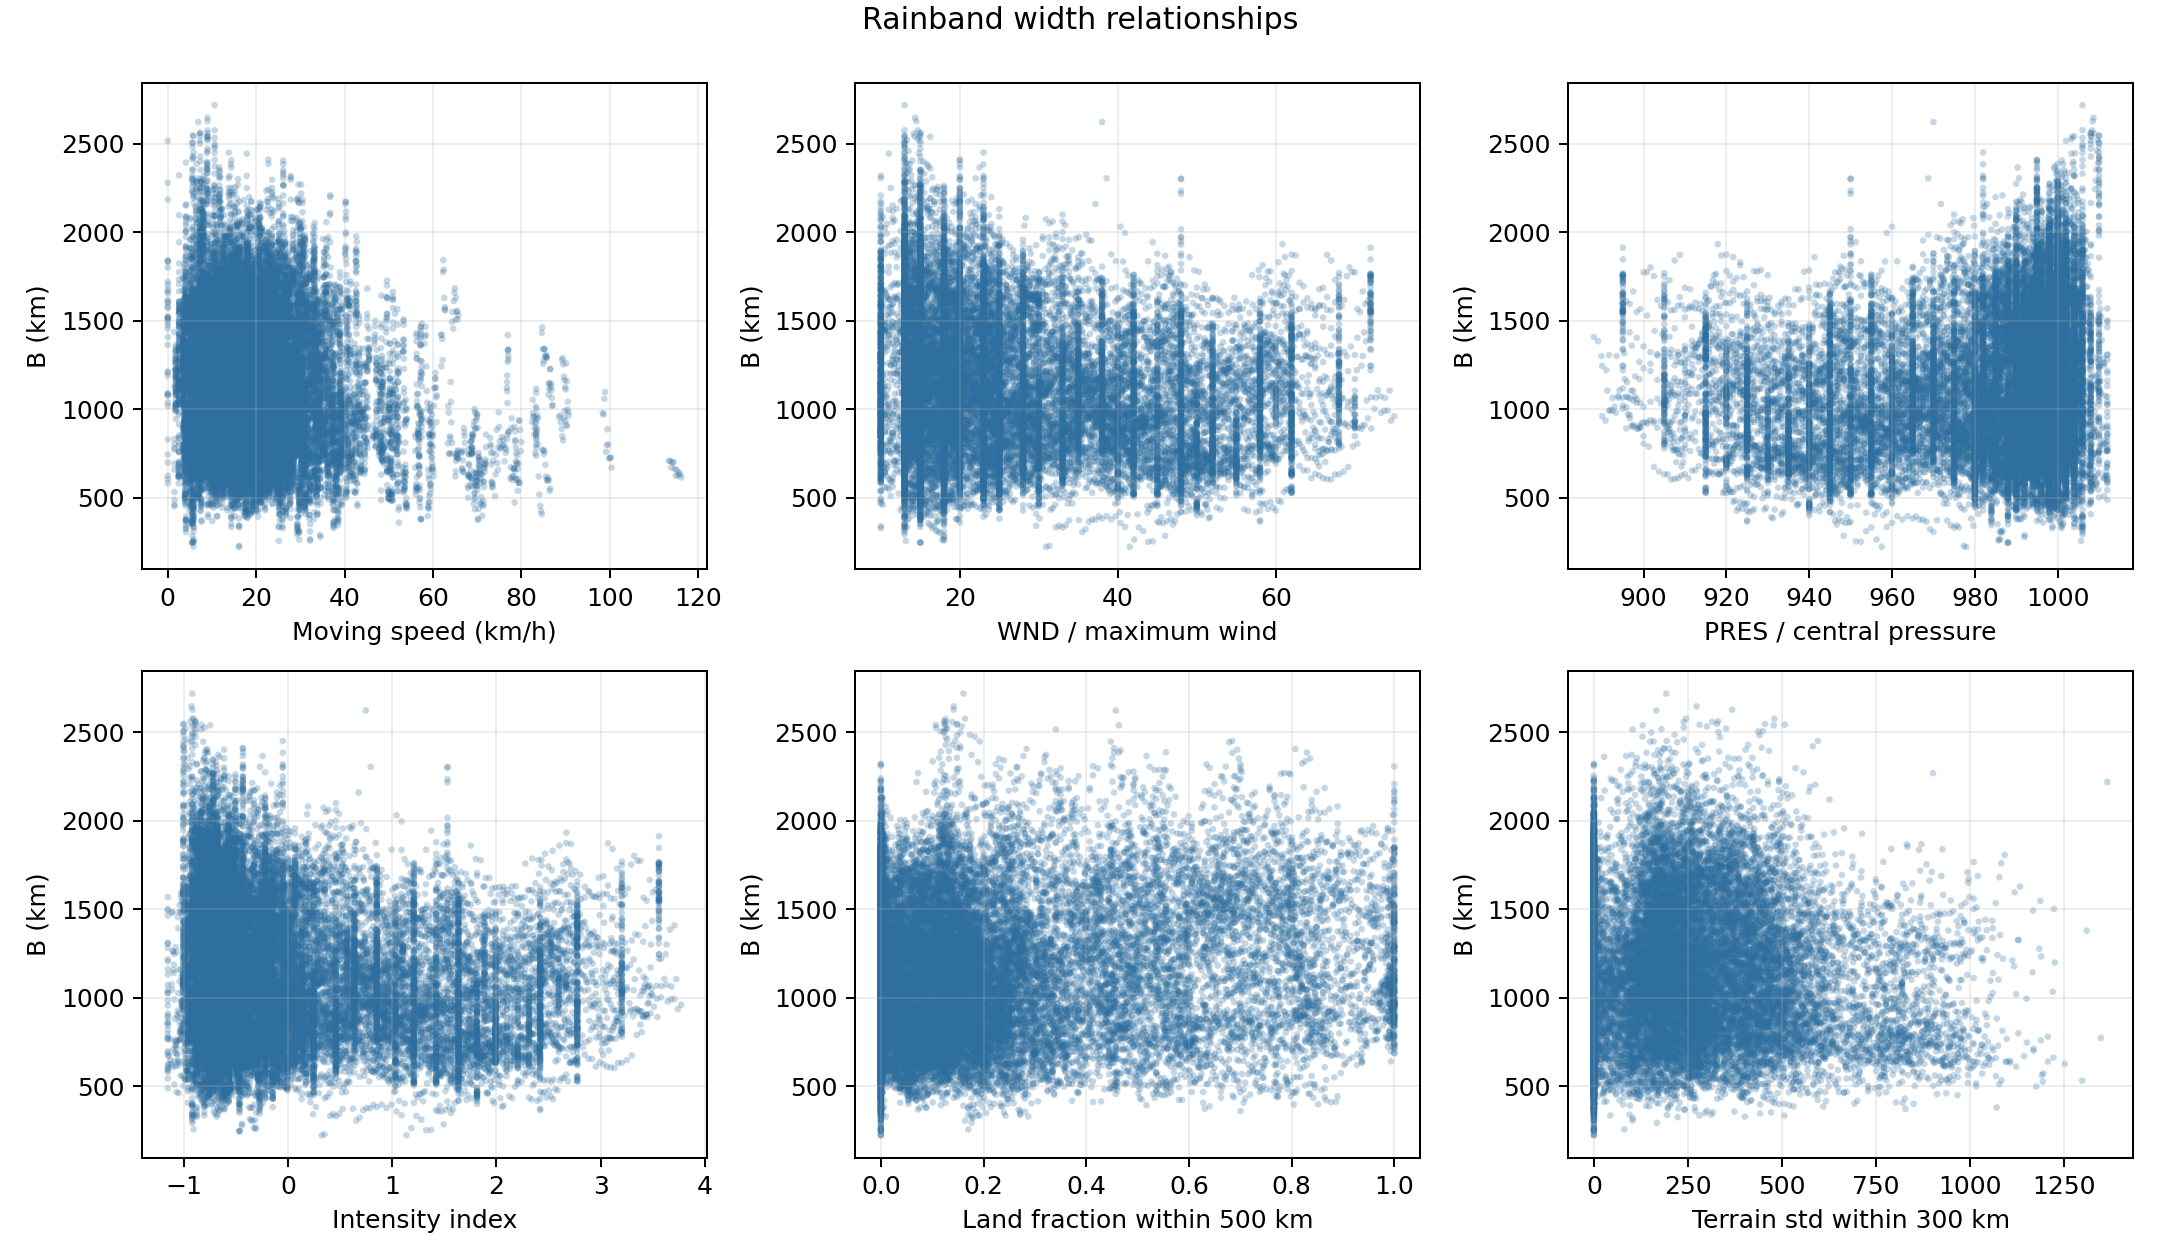
\includegraphics[width=0.95\textwidth]{outputs/figures/problem1_env/rainband_width_relationships.png}
    \caption{雨带横向等效带宽与主要路径、强度及环境变量关系}
    \label{fig:rainband_width_relationships}
\end{figure}

\subsubsection{典型历史台风演变过程综合展示}

为直接展示台风演变过程中台风特征与降水时空分布之间的关系，本文在排除 KONG-REY 和 MAN-YI 后，从问题一最终历史半小时样本中按时次数、字段完整性和指标变化幅度自动筛选代表性台风，得到 2023 年 MAWAR（CH2023\_0003）。该过程共包含 709 个半小时时次，时间范围为 2023-05-19 18:00 至 2023-06-03 12:00。图\ref{fig:typical_typhoon_evolution_problem1}给出了 MAWAR 的路径、强度、降水结构指标和四个代表时刻降水场。

\begin{figure}[htbp]
    \centering
    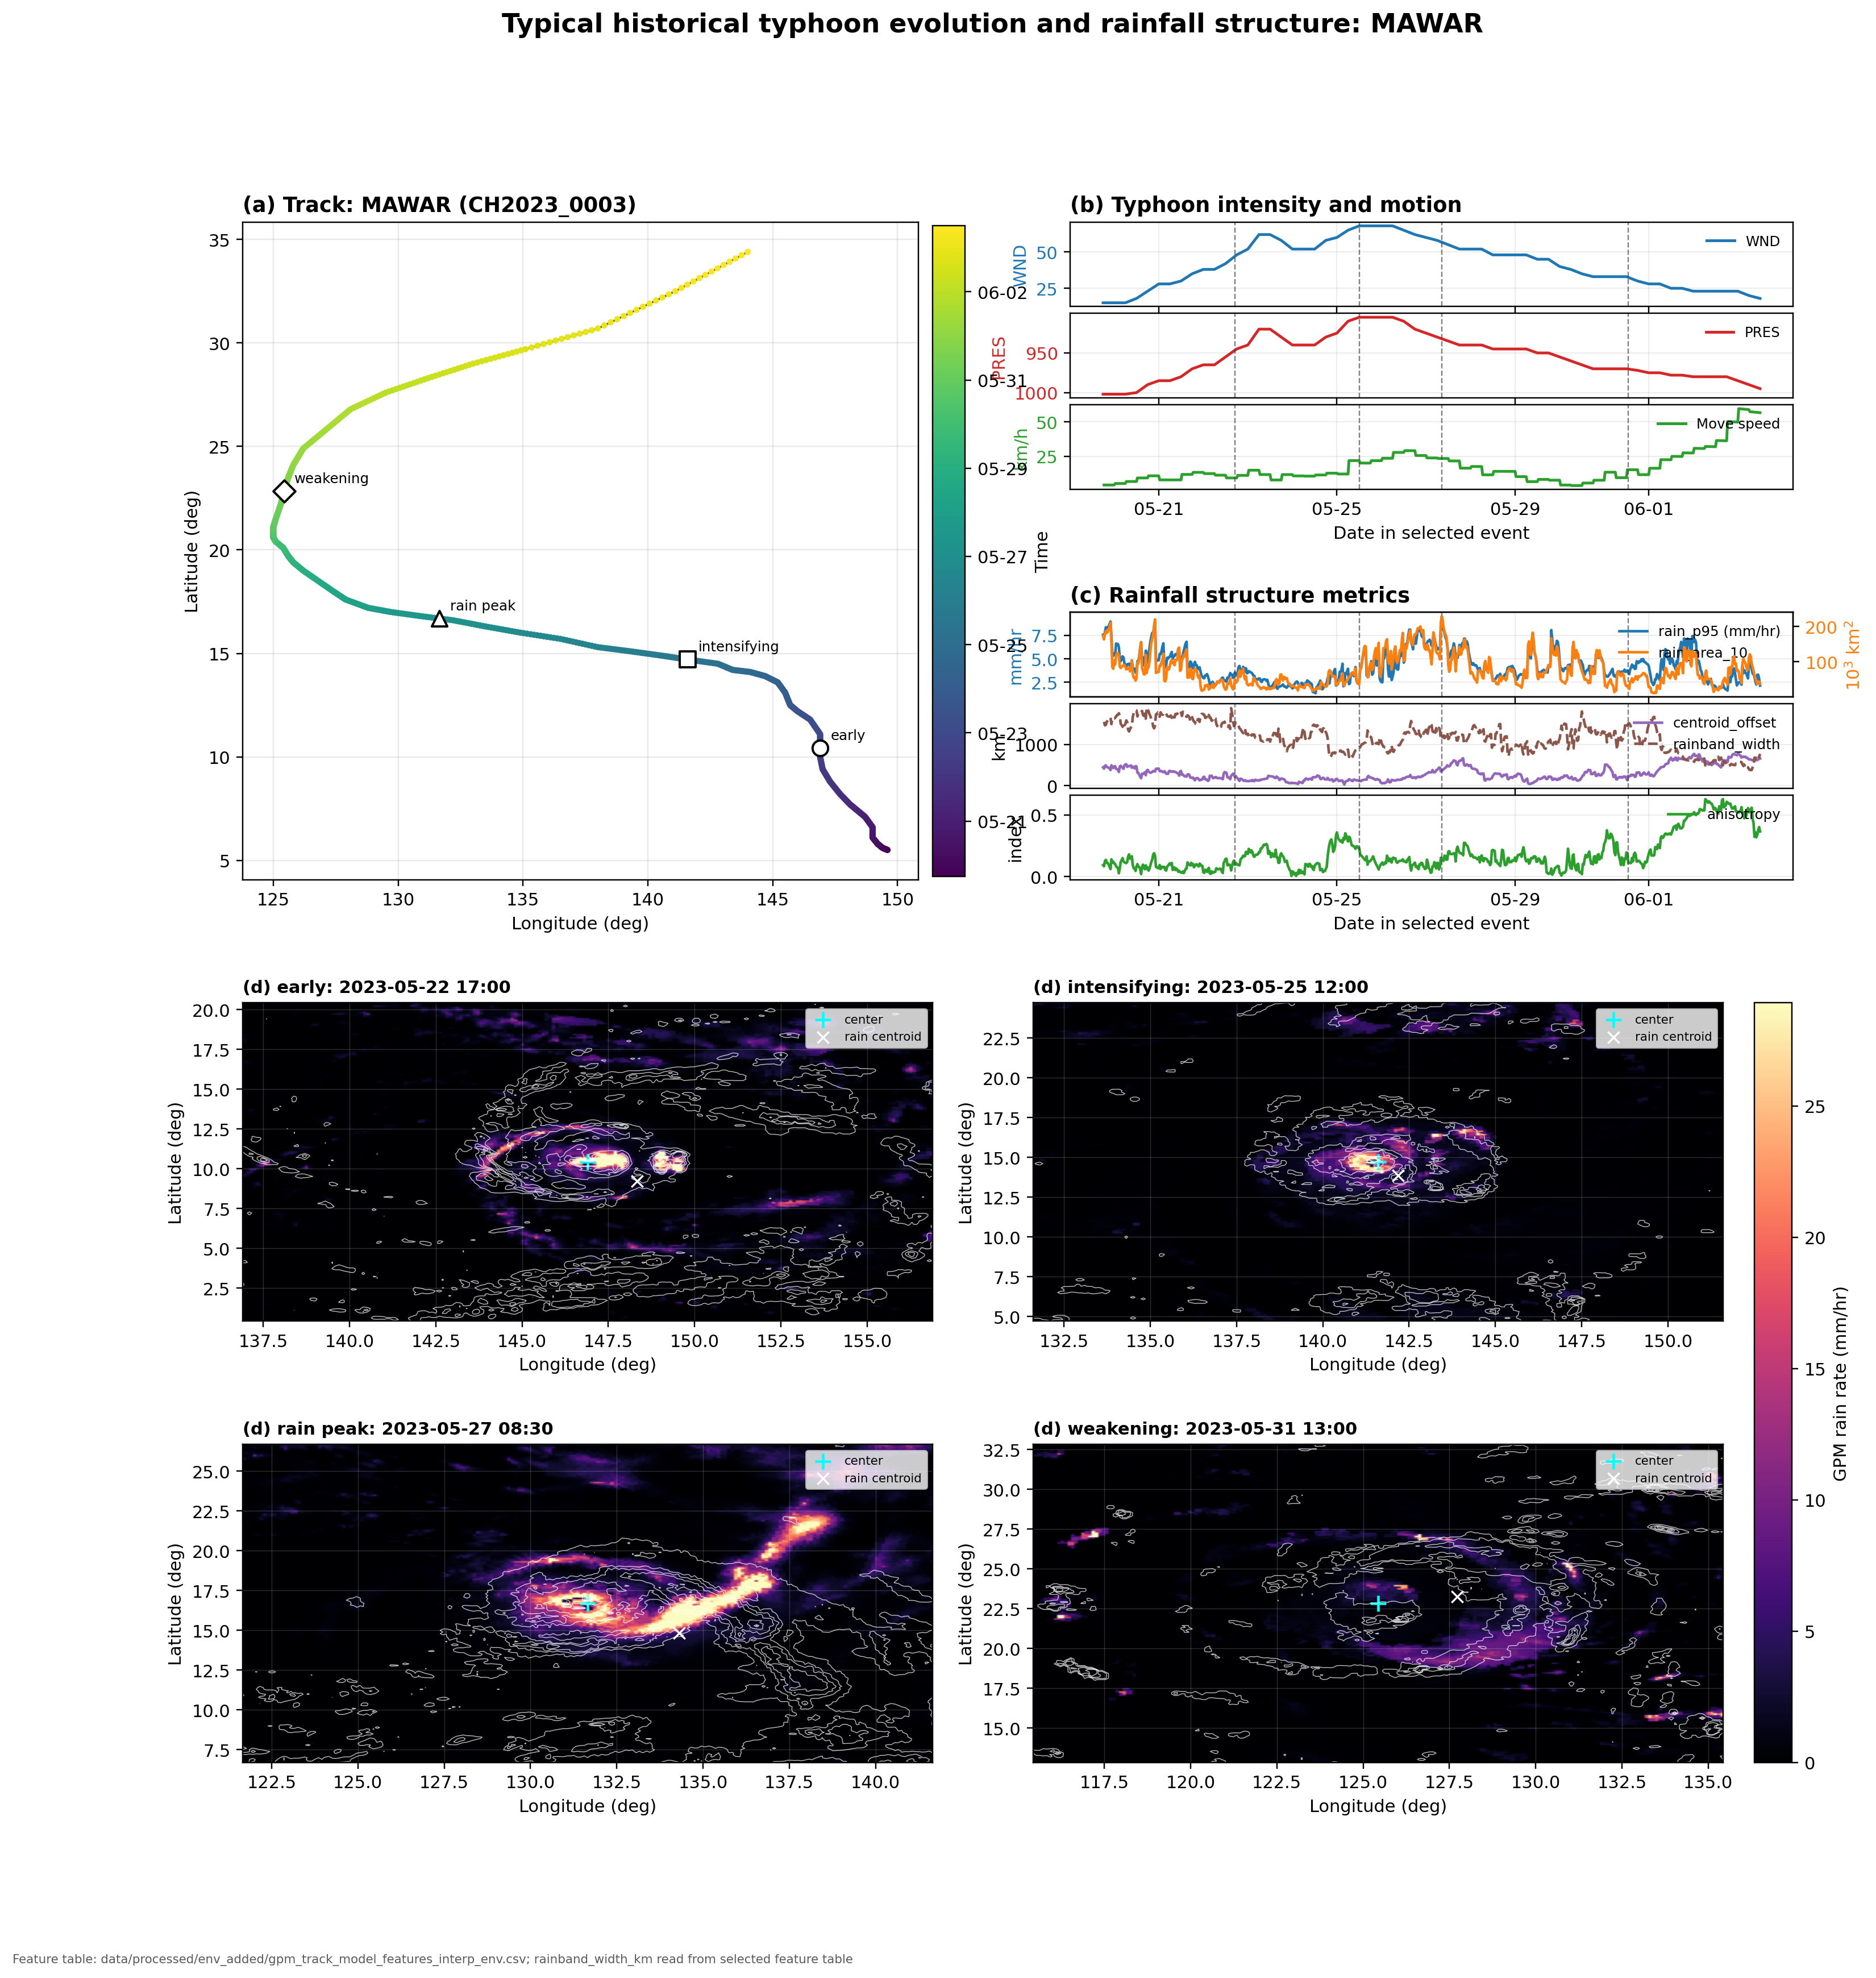
\includegraphics[width=0.98\textwidth]{outputs/figures/problem1_env/problem1_typical_typhoon_evolution.png}
    \caption{典型历史台风 MAWAR 演变过程综合图}
    \label{fig:typical_typhoon_evolution_problem1}
\end{figure}

由图\ref{fig:typical_typhoon_evolution_problem1}可见，MAWAR 前期从西北太平洋低纬海域向西北方向移动，随后在菲律宾以东海域附近转向北上并在后期继续向东北侧移动，路径转折使降水落区相对于台风中心的位置持续调整。强度演变上，MAWAR 在 2023-05-25 12:00 左右达到最强，最大风速 WND 为 68、中心气压 PRES 降至 905 hPa；但降水峰值出现在 2023-05-27 08:30，$rain\_p95$ 达到 9.53 mm/hr，$rain\_area\_10$ 达到 $2.28\times10^5\ \mathrm{km^2}$，说明强降水范围相对最大强度存在滞后。降水结构指标随时间也发生明显变化：全过程中降水质心最大偏移为 771.3 km，雨带各向异性最大为 0.628，雨带横向等效带宽最大为 1889.8 km；四个代表时刻中，生成前期雨区已围绕低纬中心组织，增强期在强风速和低气压下强降水更集中，降水峰值期雨带向台风东侧和东北侧扩展并形成最大的 P95 与强降水面积，减弱期虽然风速下降至 32.5、中心气压回升至 970.3 hPa，但雨带带宽仍约为 1504.7 km，表明衰减阶段降水强度减弱的同时，空间分布仍可保持较宽的外围雨带结构。

\subsubsection{季节背景与海陆因素的调制作用}

从随机森林重要性看，月份周期变量在多个目标变量中具有较高贡献。例如，$month\_cos$在$rain\_p95$、$rain\_area\_10\_km^2$、$centroid\_offset$和$anisotropy$模型中均排名靠前。这说明台风降水结构不仅受台风自身路径和强度影响，还受到季节背景环流和水汽供应条件的调制。不同月份西太平洋水汽输送、季风背景和副热带高压位置存在差异，这些因素会改变台风降水带的组织形态和强降水范围。

海陆、陆地覆盖和地形起伏因素也在多个模型中具有一定贡献。引入新增环境变量后，$landfrac\_500km$ 在最大降水强度、强降水面积、强降水等效半径和质心偏移等模型中均进入前十重要特征，其中在 $rain\_max$、$rain\_area\_10\_km^2$ 和强降水等效半径模型中均排名第3，在 $centroid\_offset\_km$ 模型中排名第6，在 $rain\_p95$ 模型中排名第9。$terrain\_std\_300km$ 在雨带各向异性模型中排名第5，同时 $landfrac\_500km$ 在该模型中排名第7。上述结果说明，较大尺度陆地覆盖背景能够补充单一距岸距离变量，对强降水范围和降水中心偏移具有调制作用；台风中心附近地形起伏复杂度则会影响雨带形态和空间不均匀性。

新增环境变量与主要降水指标的 Spearman 相关系数如表\ref{tab:env_spearman_problem1}所示。

\begin{table}[htbp]
    \centering
    \caption{新增环境变量与主要降水指标的Spearman相关系数}
    \label{tab:env_spearman_problem1}
    \small
    \begin{tabular}{lrrrrr}
        \hline
        环境变量 & $rain\_p95$ & $rain\_area\_10\_km^2$ & $centroid\_offset$ & $anisotropy$ & $B$ \\
        \hline
        $landfrac\_200km$ & -0.0175 & -0.1266 & 0.0894 & 0.0163 & 0.0478 \\
        $landfrac\_500km$ & -0.0167 & -0.1393 & 0.0946 & 0.0246 & 0.0511 \\
        $terrain\_mean\_300km$ & 0.0003 & -0.0575 & 0.0425 & 0.0586 & -0.0055 \\
        $terrain\_max\_300km$ & 0.0028 & -0.0623 & 0.0499 & 0.0572 & 0.0055 \\
        $terrain\_std\_300km$ & 0.0029 & -0.0553 & 0.0420 & 0.0509 & 0.0052 \\
        \hline
    \end{tabular}
\end{table}

由表\ref{tab:env_spearman_problem1}可见，新增环境变量与主要降水指标的 Spearman 相关性整体不强，说明 $landfrac$ 和 $terrain$ 类变量并非以简单线性或单调关系影响降水结构；但随机森林中这些变量具有较高置换重要性，说明其作用主要通过与台风强度、移动方向、季节背景和近岸过程的非线性交互体现。因此，本文将海陆覆盖和地形变量定位为降水结构的调制因子，而非唯一主控因子。

\subsection{主要影响因素综合排序}

为了进一步比较不同目标变量的主控因子，本文整理随机森林置换重要性排名前五的变量，如表\ref{tab:rf_top_factors_problem1}所示。

\begin{table}[htbp]
    \centering
    \caption{不同降水分布特征的主要影响因素}
    \label{tab:rf_top_factors_problem1}
    \begin{tabular}{p{0.25\textwidth}p{0.62\textwidth}c}
        \hline
        响应变量 & 随机森林重要性前五变量 & 测试集$R^2$ \\
        \hline
        $rain\_max$ & 移动方向正弦、最大风速、$landfrac\_500km$、移动速度、气压亏损 & 0.409 \\
        $rain\_p95$ & 移动方向正弦、月份余弦、综合强度指数、移动方向余弦、中心气压 & 0.666 \\
        $rain\_area\_10\_km^2$ & 移动方向正弦、最大风速、$landfrac\_500km$、气压亏损、移动方向余弦 & 0.614 \\
        强降水等效半径 & 最大风速、移动方向正弦、$landfrac\_500km$、月份余弦、气压亏损 & 0.665 \\
        降水质心偏移 & 移动方向正弦、移动速度、综合强度指数、月份余弦、移动方向余弦 & 0.684 \\
        雨带各向异性 & 移动方向正弦、月份余弦、移动速度、移动方向余弦、$terrain\_std\_300km$ & 0.640 \\
        雨带带宽 & 移动方向正弦、月份余弦、移动速度、$landfrac\_500km$、最大风速 & 0.708 \\
        \hline
    \end{tabular}
\end{table}

由表\ref{tab:rf_top_factors_problem1}可知，移动方向正弦在所有主要目标变量中均排名靠前，说明台风降水分布对台风路径方向具有显著依赖。强度相关变量主要控制降水强度和强降水范围；移动速度和移动方向主要控制降水质心偏移、雨带各向异性和雨带带宽；月份周期变量在多个目标变量中均有贡献，表明季节背景不可忽略；$landfrac\_500km$ 和 $terrain\_std\_300km$ 的进入表明海陆覆盖与地形起伏能够在非线性模型中补充距岸距离信息。进一步在台风相对运动坐标系下计算前后、左右和四象限降水比例后，可以发现历史台风降水总体偏向运动前方和左侧，这进一步说明降水非对称性并非固定的东西南北偏向，而是与台风动力过程、移动方向和周边下垫面条件密切相关。

\subsection{模型检验与进一步讨论}

为检验模型是否仅仅拟合同一台风事件内部的连续演变，本文设置两种验证方式。第一种为普通随机划分，即随机抽取半小时时次样本进入训练集和测试集；第二种为按台风事件分组划分，即以$track\_event\_uid$为分组单位，保证同一场台风不会同时出现在训练集和测试集中。前者主要检验模型对同一台风过程内部降水演变规律的解释能力，后者则更接近对未知台风事件的外推检验。两种验证方式的结果如表\ref{tab:random_vs_group_validation_problem1}所示。

\begin{table}[htbp]
    \centering
    \caption{普通随机划分与按台风事件分组划分的模型验证结果对比}
    \label{tab:random_vs_group_validation_problem1}
    \small
    \begin{tabular}{lrrrr}
        \hline
        指标 & 随机划分$R^2$ & 按台风分组$R^2$ & $R^2$下降 & MAE增幅/\% \\
        \hline
        最大降水强度 & 0.409 & -0.031 & 0.440 & 42.6 \\
        95分位降水强度 & 0.666 & 0.032 & 0.633 & 91.0 \\
        强降水面积 & 0.614 & 0.039 & 0.575 & 75.3 \\
        强降水等效半径 & 0.665 & 0.079 & 0.586 & 81.6 \\
        降水中心偏移距离 & 0.684 & -0.112 & 0.795 & 91.2 \\
        雨带各向异性 & 0.640 & 0.017 & 0.624 & 67.1 \\
        雨带带宽 & 0.708 & -0.015 & 0.723 & 101.1 \\
        \hline
    \end{tabular}
\end{table}

由表\ref{tab:random_vs_group_validation_problem1}可见，在普通随机划分下，引入环境变量后的增强随机森林模型对95分位降水强度、强降水面积、强降水等效半径、降水中心偏移距离和雨带各向异性均具有较高解释能力，测试集$R^2$大多在0.61以上。这说明路径、强度、移动方向、季节背景、海陆覆盖和地形环境能够较好刻画同一台风过程内部的降水结构演变。与未加入新增环境变量的版本相比，普通随机划分下各目标$R^2$均略有提升；按台风事件分组验证中，除 $rain\_p95$ 分组$R^2$小幅下降约0.003外，其余目标多数改善，说明新增环境变量没有导致事件外推检验的整体恶化。

然而，在按台风事件分组划分后，测试集$R^2$仍明显下降，其中部分目标变量的$R^2$接近0或为负，MAE也显著增加。这表明当测试集为模型从未见过的台风事件时，仅依赖路径、强度、近岸、陆地覆盖、地形和时间背景变量仍难以稳定外推逐时降水结构。换言之，不同台风事件之间存在显著个体差异，台风降水还受到水汽输送、垂直风切变、背景环流、海温等因素的影响。

该检验结果具有重要意义：问题一中的随机森林模型更适合用于解释历史台风过程中路径、强度和环境因素对降水分布的影响规律，而不宜直接作为问题二中KONG-REY和MAN-YI的逐格降水生成模型。因此，在后续问题二中，本文不采用简单监督回归直接预测目标台风降水场，而采用“相似历史时次筛选—台风相对坐标下降水模板迁移—强度、极端分位数与近岸因子校准”的生成思路。同时，由于问题一结果表明降水结构具有明显的台风相对运动方向偏向，后续模板迁移将在台风相对运动坐标系下进行，以避免直接在经纬度坐标中比较不同路径方向台风导致的结构错位。

需要特别说明的是，问题一中提取的降水结构特征变量，如
$\mathrm{rain\_p95}$、$\mathrm{rain\_area\_10\_km^2}$、$\mathrm{centroid\_offset}$、$\mathrm{anisotropy}$、$\mathrm{rainband\_width\_km}$，
以及前后向、左右向降水比例等，均由GPM降水场计算得到。然而，由于台风KONG-REY和MAN-YI在GPM数据集中不存在对应的降水记录，上述降水结构变量在问题二中无法作为目标台风的输入特征使用。因此，这些变量仅用于历史样本的输出指标描述、生成结果的校准目标以及模型合理性的检验依据。问题二的模型输入仅选取目标台风可直接获取或可由路径数据派生的变量，包括路径特征（位置、移动速度与方向）、强度特征（气压、风速）、时间季节特征，以及环境特征（海陆分布、近岸距离等）。

综上，模型检验表明：本文所建问题一模型能够较好解释同一台风过程内部的降水时空演变规律，并能识别影响降水强度、范围、质心偏移和雨带形态的主要因素；但对于完全未知的台风事件，单纯依靠路径和强度变量进行逐时外推存在明显局限。因此，问题一模型在全文中的定位是“关系解释与特征筛选模型”，其结论为问题二中相似样本筛选、降水模板迁移和生成结果校准提供依据。


\subsection{问题一结论}

综合以上分析，得到如下结论：

\begin{enumerate}
    \item 台风强度是影响降水强度和强降水范围的主控因子。中心气压越低、气压亏损越大、最大风速越强，P95降水强度和强降水面积越大。
    \item 台风移动方向和移动速度显著影响降水空间结构。移动方向正弦和余弦特征在多个模型中排名靠前，说明降水质心偏移、非对称性、雨带各向异性和降水带宽均具有明显路径方向依赖。
    \item 在台风相对运动坐标系下，降水总体偏向移动前方和左侧。前左象限为平均降水比例最大的区域，且$10\ \mathrm{mm/hr}$以上强降水面积也主要集中在前方和左侧，说明台风降水非对称性与台风移动方向密切相关。
    \item 台风增强或减弱过程会改变降水非对称性。风速变化率和气压变化率与东西、南北非对称性存在较明显相关，说明降水偏向不仅由当前强度决定，还与台风演变趋势有关。
    \item 季节背景是不可忽略的调制因子。月份周期变量在多个模型中具有较高重要性，说明水汽供应和背景环流条件会影响台风降水强度、范围和雨带形态。
    \item 海陆与距岸因素对降水结构具有调制作用。距岸距离和近岸影响指数对强降水范围、降水质心偏移、雨带各向异性和雨带横向扩展具有一定贡献，但其作用通常弱于强度、移动方向和季节背景。
    \item 本文补充的陆地覆盖比例和地形起伏变量对降水空间结构具有非线性调制作用。其中，500 km陆地覆盖比例对强降水面积、强降水等效半径和降水质心偏移具有较强解释贡献；300 km地形起伏标准差对雨带各向异性具有一定贡献。这说明台风降水空间结构不仅受路径、强度和移动因素影响，也受到周边下垫面和地形起伏的调制。
\end{enumerate}

\section{问题二模型的建立与求解}

问题二要求在 KONG-REY 和 MAN-YI 两场台风没有 GPM 降水记录的条件下，依据历史台风的“路径--强度--环境--降水”关系生成其可能的半小时降水时空分布。因此，本问不是普通的标量预测问题，而是一个条件降水场生成问题。本文将生成过程分解为七个环节：历史半小时样本库构建、目标台风安全输入构造、历史相似时次检索、台风相对坐标模板迁移、EOF/PCA 大尺度结构修正、极端分位数校准和历史台风伪缺失验证。最终以极端校准后的降水场作为 KONG-REY 与 MAN-YI 的可能降水分布结果。

\subsection{建模思路与安全输入说明}

由于 KONG-REY 和 MAN-YI 在 GPM 降水数据集中没有真实降水记录，模型输入必须严格限定为目标台风在生成时可获得的信息，包括路径、强度、移动、时间和海陆环境特征。本文将由历史 GPM 降水场计算得到的降水指标仅作为历史标签、模板校准目标和验证指标，而不作为目标台风输入，以避免数据泄漏。

为避免目标台风名称、时间窗或路径样本发生误配，本文首先对 KONG-REY 和 MAN-YI 的目标输入表进行匹配核验，结果见表~\ref{tab:p2_target_match_check}。核验同时依据 CMABST 事件编号和台风名称在已完成路径匹配的 GPM 样本表中查找对应记录，结果均为不存在。因此，后续模型不把相邻时段其他台风的 GPM 降水场误认为目标台风观测，而是仅使用目标台风路径、强度、移动和近岸环境等安全变量进行条件降水场生成。

\begin{table}[H]
  \centering
  \caption{KONG-REY 与 MAN-YI 目标台风匹配核验}
  \label{tab:p2_target_match_check}
  \small
  \resizebox{\textwidth}{!}{
  \begin{tabular}{l c c c c c c c}
    \toprule
    名称 & 时间窗 & 时次数 & 经度范围 & 纬度范围 & 最大风速/(m/s) & 最低气压/hPa & GPM 是否存在 \\
    \midrule
    KONG-REY & 2024-10-24 18:00--2024-11-02 12:00 & 421 & 119.9--146.5$^\circ$E & 12.8--34.7$^\circ$N & 60.0 & 920.0 & 不存在 \\
    MAN-YI & 2024-11-08 12:00--2024-11-20 00:00 & 553 & 111.0--163.6$^\circ$E & 10.4--18.8$^\circ$N & 62.0 & 920.0 & 不存在 \\
    \bottomrule
  \end{tabular}
  }
\end{table}

对任一目标半小时时刻 $t$，构造安全输入向量
\begin{equation}
\boldsymbol{X}_t=
\left[
\varphi_t,\lambda_t,WND_t,PRES_t,I_t,U_t,
\sin \alpha_t,\cos \alpha_t,
\Delta WND_t,\Delta PRES_t,
I_t^{land},d_t^s,d_t^a,
\sin m_t,\cos m_t,p_t
\right],
\end{equation}
其中，$\varphi_t,\lambda_t$ 分别为台风中心纬度和经度，$WND_t$ 为最大风速字段，$PRES_t$ 为中心最低气压，$I_t$ 为强度等级，$U_t$ 为移动速度，$\alpha_t$ 为移动方向，$\Delta WND_t,\Delta PRES_t$ 为强度变化率，$I_t^{land}$ 为是否登陆或陆地标记，$d_t^s$ 为有符号距岸距离，$d_t^a$ 为距岸距离绝对值，$m_t$ 为月份，$p_t$ 为生命周期进程。由于路径数据中 OWD 字段缺失，本文不使用 OWD。

历史半小时样本库共包含 $32842$ 个历史时次、$88$ 个字段，每行对应一个历史台风的一个半小时时刻。问题一中完成路径匹配的 GPM 半小时时次数为 $33420$；问题二构建历史模板库时，为避免目标台风降水信息泄漏，将 2024 年目标台风名称或目标时间窗对应的 $578$ 个 GPM 半小时时次从历史库中排除，剩余样本全部成功入库，因此最终得到 $32842$ 个可用于相似检索和模板迁移的历史半小时时次。目标台风安全输入采用完成环境重算后的 leakage-safe 输入表，而不使用缺少经纬度字段的目标台风对齐表。目标台风安全输入表共包含 $974$ 个半小时时刻，其中 KONG-REY 包含 $421$ 个时刻，时间范围为 2024-10-24 18:00:00 至 2024-11-02 12:00:00；MAN-YI 包含 $553$ 个时刻，时间范围为 2024-11-08 12:00:00 至 2024-11-20 00:00:00。

需要特别说明的是，以下由 GPM 降水场计算得到的字段均不参与目标台风输入和相似检索：
\begin{equation}
\texttt{rain\_*},\quad
\texttt{centroid\_*},\quad
\texttt{quad\_*},\quad
\texttt{anisotropy},\quad
\texttt{rain\_radius\_*},\quad
\texttt{rain\_band\_width}.
\end{equation}
这些字段只用于历史样本描述、极端分位数校准和伪缺失验证。本文根据题目要求补充陆地覆盖比例和地形高程类环境变量，包括 $landfrac\_200km$、$landfrac\_500km$、$terrain\_mean\_300km$、$terrain\_max\_300km$ 和 $terrain\_std\_300km$。问题一解释模型表明，上述变量对强降水面积、降水质心偏移和雨带各向异性具有非线性调制作用。进一步在问题二伪缺失验证中进行环境变量消融实验后发现，加入全部新增环境变量未能稳定提升降水生成效果。因此，为保证新台风生成的稳健性，问题二最终相似检索中的环境距离仍采用 \texttt{is\_land}、\texttt{signed\_coast\_dist\_km} 和 \texttt{coast\_dist\_km}；新增环境变量作为机理解释、模型消融和第三问虚拟路径情景重算的辅助环境信息。同时，本文在消融实验中将 $landfrac\_200km$、$landfrac\_500km$、$terrain\_mean\_300km$、$terrain\_max\_300km$、$terrain\_std\_300km$ 作为候选环境输入进行检验，最终根据伪缺失验证结果决定是否纳入最终生成模型。

\subsection{历史相似样本检索模型}

\subsubsection{安全特征标准化}

对每个目标时刻 $t$，本文从历史样本库中检索与其路径、强度、移动、季节和海陆环境最相似的历史半小时时次。所有连续变量均使用历史库均值与标准差进行标准化：
\begin{equation}
z_j(x)=\frac{x-\mu_j}{\sigma_j+\varepsilon},
\end{equation}
其中 $\mu_j,\sigma_j$ 分别为历史库中特征 $j$ 的均值和标准差，$\varepsilon$ 为防止除零的小常数。移动方向采用 $\sin \alpha$ 和 $\cos \alpha$ 表示，避免角度循环造成的距离误差。

\subsubsection{分量距离与总距离}

本文将相似距离分解为六个部分：
\begin{align}
D_{\mathrm{track}} &= \operatorname{mean}\left[
\Delta z(\varphi)^2,\Delta z(\lambda)^2
\right],\\
D_{\mathrm{intensity}} &= \operatorname{mean}\left[
\Delta z(WND)^2,\Delta z(PRES)^2,\Delta z(I)^2
\right],\\
D_{\mathrm{motion}} &= \operatorname{mean}\left[
\Delta z(U)^2,\Delta z(\sin\alpha)^2,\Delta z(\cos\alpha)^2,
\Delta z(\Delta WND)^2,\Delta z(\Delta PRES)^2
\right],\\
D_{\mathrm{env}} &= \operatorname{mean}\left[
\Delta z(I^{land})^2,\Delta z(d^s)^2,\Delta z(d^a)^2
\right],\\
D_{\mathrm{time}} &= \operatorname{mean}\left[
\Delta z(\sin m)^2,\Delta z(\cos m)^2
\right],\\
D_{\mathrm{life}} &= \Delta z(p)^2.
\end{align}
总距离定义为
\begin{equation}
D(t,s)=
1.0D_{\mathrm{track}}
+1.5D_{\mathrm{intensity}}
+1.2D_{\mathrm{motion}}
+1.2D_{\mathrm{env}}
+0.8D_{\mathrm{time}}
+0.8D_{\mathrm{life}},
\end{equation}
其中 $s$ 表示历史候选时次。若某类特征整体缺失，则自动跳过该特征，并对该分量按实际可用特征数取平均，避免某一类变量因字段数较多而天然占据更高权重。

上述距离分量权重并非任意设定，而是依据问题一中变量解释结果和台风降水物理含义确定。问题一的结果表明，强度变量（WND、PRES）对 $R_{95}$、$R_{99}$ 以及强降水面积具有稳定影响，因此本文对强度分量赋予较高权重 $1.5$；移动速度和移动方向直接影响降水质心偏移、前后/左右非对称性和雨带各向异性，因此移动分量权重设为 $1.2$，略高于单纯路径位置分量；近岸距离和是否登陆等海陆环境变量会改变台风降水的空间范围和雨带形态，因此环境分量同样设为 $1.2$；月份变量主要反映背景水汽条件和季节环流差异，作为辅助筛选因素，权重设为 $0.8$；生命周期进程用于避免将台风初生阶段、成熟阶段和减弱阶段错误匹配，也作为辅助约束，权重设为 $0.8$。由此，本文相似距离既强调强度和移动结构对降水场的主导作用，又保留季节和生命周期对历史样本匹配的修正作用。进一步地，表 \ref{tab:p2_sensitivity_result} 的敏感性分析表明，关键参数扰动下模型性能未出现明显突变，说明该权重设置具有一定鲁棒性。

为检验补充海陆覆盖比例和地形变量是否能够提升问题二降水生成效果，本文在伪缺失验证框架下设置三组环境距离对比实验：
\begin{enumerate}
    \item Base-old：仅使用是否登陆、有符号距岸距离和距岸距离；
    \item Env-full：在 Base-old 基础上加入 $landfrac\_200km$、$landfrac\_500km$、$terrain\_mean\_300km$、$terrain\_max\_300km$、$terrain\_std\_300km$；
    \item Env-key：在 Base-old 基础上仅加入问题一解释贡献较突出的 $landfrac\_500km$ 和 $terrain\_std\_300km$。
\end{enumerate}
三组设置除环境距离变量外，其余相似检索、模板迁移、EOF/PCA 修正和极端校准参数均保持一致。后文环境变量消融结果表明，Base-old 在极端降水恢复指标上表现更稳健，因此本文最终主模型采用上述 $D_{\mathrm{env}}$ 设置。

对每个目标时刻，选取距离最小的 $K=20$ 个历史时次作为相似样本。为避免相似样本被某一场历史台风垄断，设置同一历史事件在单个目标时刻的 Top-$K$ 中最多出现 $3$ 次。最终每个目标时刻的 Top-$K$ 中唯一历史台风事件数均值为 $7.165$，最小值为 $7$，说明相似模板来源具有一定多样性。

\subsubsection{相似权重}

对选出的 Top-$K$ 历史样本，采用 softmax 距离权重：
\begin{equation}
\omega_j(t)=
\frac{\exp[-D(t,s_j)/\tau_t]}
{\sum_{k=1}^{K}\exp[-D(t,s_k)/\tau_t]},
\end{equation}
其中 $\tau_t$ 取该目标时刻 Top-$K$ 距离的中位数。最终得到 $974\times 20=19480$ 条目标--历史相似样本匹配记录，每个目标时刻均有 $20$ 个历史相似样本，且权重和为 $1$。相似距离的中位数为 $1.156$，$95\%$ 分位数为 $2.345$。Top-$K$ 历史样本中不包含 KONG-REY、MAN-YI 及其目标时间窗样本。

\subsection{\texorpdfstring{storm-relative}{storm-relative} 模板迁移生成模型}

\subsubsection{台风相对运动坐标系}

直接在经纬度坐标下比较不同台风的降水场会混淆移动方向差异。为统一不同台风的雨带结构，本文将历史 GPM 降水场转换到台风相对运动坐标系。设台风中心为 $(\lambda_c,\varphi_c)$，原始相对坐标中的 $x$ 表示向东距离，$y$ 表示向北距离：
\begin{equation}
x=111.32\cos(\varphi_c)(\lambda-\lambda_c),\qquad
y=111.32(\varphi-\varphi_c).
\end{equation}
设 $\alpha$ 为台风移动方向角，$0^\circ$ 表示正北，$90^\circ$ 表示正东。定义
\begin{equation}
x_f=x\sin\alpha+y\cos\alpha,\qquad
y_l=-x\cos\alpha+y\sin\alpha,
\end{equation}
其中 $x_f>0$ 表示台风移动前方，$y_l>0$ 表示移动方向左侧。本文采用统一相对坐标网格：
\begin{equation}
x_f,y_l\in[-1000,1000]\ \mathrm{km},\qquad
201\times 201.
\end{equation}

\subsubsection{Top-$K$ 模板加权生成}

对每个目标时刻 $t$，读取其 Top-$K$ 历史样本的 GPM 降水场 $R_{s_j}$，重采样到上述台风相对运动坐标网格。为减弱极端值对加权平均的影响，并保证雨场非负，本文在 $\log(1+R)$ 空间进行模板迁移：
\begin{equation}
G_t^{(0)}(x_f,y_l)
=
\sum_{j=1}^{K}\omega_j(t)\log\left[1+R_{s_j}(x_f,y_l)\right],
\end{equation}
\begin{equation}
R_t^{(0)}(x_f,y_l)
=
\exp\left(G_t^{(0)}(x_f,y_l)\right)-1.
\end{equation}
这里 $R_t^{(0)}$ 为初始生成场，单位为 \(\mathrm{mm/hr}\)。若计算半小时累计量，则使用 $0.5R_t^{(0)}$。

初始场共生成 $974$ 个半小时时次，数组维度为 $(974,201,201)$，没有 NaN、Inf、负值或全零场。其最大格点降水 $R_{\max}$ 的中位数、$95\%$ 分位数和最大值分别为 $8.178$、$23.329$ 和 $29.443\ \mathrm{mm/hr}$。但初始场相对于 Top-$K$ 历史样本加权最大值的比值中位数仅为 $0.184$，表明 $\log(1+R)$ 加权平均虽能较好保留大尺度雨区形态，但会明显平滑局地极端降水。因此后续需要引入极端分位数校准。

\subsection{EOF/PCA 大尺度结构修正}

\subsubsection{EOF/PCA 空间模态分解}

为增强生成雨场的大尺度结构稳定性和可解释性，本文进一步对历史相似模板进行 EOF/PCA 分解。选取目标相关的唯一 Top-$K$ 历史模板作为训练集，共 $2166$ 个历史相似降水模板。对每个模板取
\begin{equation}
G_s(x_f,y_l)=\log\left[1+R_s(x_f,y_l)\right],
\end{equation}
并在 $\log(1+R)$ 空间进行 PCA 分解：
\begin{equation}
G_s(x_f,y_l)
\approx
\mu(x_f,y_l)+
\sum_{k=1}^{K_{\mathrm{EOF}}}a_{k,s}\phi_k(x_f,y_l),
\end{equation}
其中 $\mu$ 为历史平均场，$\phi_k$ 为第 $k$ 个 EOF 空间模态，$a_{k,s}$ 为对应系数。本文取 $K_{\mathrm{EOF}}=20$。前五个 EOF 模态的解释率分别为
\[
0.1037,\quad 0.0850,\quad 0.0516,\quad 0.0447,\quad 0.0304,
\]
20 个 EOF 模态累计解释率为 $0.5007$。这说明 EOF/PCA 模态主要刻画台风降水的大尺度空间结构，而不试图完全还原局地极端雨强。

\subsubsection{目标初始场投影与 EOF 重构}

对目标台风的初始场 $R_t^{(0)}$，令
\begin{equation}
G_t^{(0)}=\log\left(1+R_t^{(0)}\right).
\end{equation}
将其投影到 EOF 空间，得到目标 EOF 系数：
\begin{equation}
\hat a_{k,t}
=
\left\langle
G_t^{(0)}-\mu,\phi_k
\right\rangle.
\end{equation}
由此得到 EOF 重构场：
\begin{equation}
G_t^{\mathrm{EOF}}
=
\mu+\sum_{k=1}^{K_{\mathrm{EOF}}}\hat a_{k,t}\phi_k,
\end{equation}
\begin{equation}
R_t^{\mathrm{EOF}}
=
\exp\left(G_t^{\mathrm{EOF}}\right)-1.
\end{equation}

由于 EOF/PCA 重构也可能削弱局地极端降水，本文不直接以 $R_t^{\mathrm{EOF}}$ 作为生成结果，而采用保守融合：
\begin{equation}
R_t^{\mathrm{blend}}
=
(1-\beta)R_t^{(0)}+\beta R_t^{\mathrm{EOF}},
\qquad \beta=0.3.
\end{equation}
其中 $R_t^{\mathrm{blend}}$ 为大尺度结构修正场。结果表明，$R_t^{\mathrm{blend}}$ 与 $R_t^{(0)}$ 的空间相关系数中位数为 $0.995$，$95\%$ 分位数为 $0.998$，说明 EOF/PCA 修正没有破坏初始模板场的主要结构。$R_t^{\mathrm{blend}}$ 相对于初始场最大雨强的比值中位数为 $0.884$，说明 $\beta=0.3$ 的融合方式较为保守。

\subsection{极端分位数校准}

\subsubsection{校准与验证目标构造}

由上一节可知，模板加权和 EOF/PCA 修正均可能削弱局地极端降水。为使生成结果更符合历史相似台风的极端分布，本文以 Top-$K$ 历史样本的 P95 和 P99 作为直接校准目标，同时计算 $A_{10}$ 和 $A_{20}$ 作为强降水面积合理性的辅助检验指标。由于强降水面积与雨场空间结构密切相关，若直接强制匹配面积，可能破坏模板迁移得到的雨带形态，因此本文不对 $A_{10}$ 和 $A_{20}$ 做硬约束，而在校准后检验其误差变化。对每个目标时刻 $t$，计算：
\begin{align}
T_{95,t} &= \sum_{j=1}^{K}\omega_j(t)Q_{0.95}(R_{s_j}),\\
T_{99,t} &= \sum_{j=1}^{K}\omega_j(t)Q_{0.99}(R_{s_j}),\\
T_{\max,t} &= \sum_{j=1}^{K}\omega_j(t)\max(R_{s_j}),\\
T_{A10,t} &= \sum_{j=1}^{K}\omega_j(t)A_{10}(R_{s_j}),\\
T_{A20,t} &= \sum_{j=1}^{K}\omega_j(t)A_{20}(R_{s_j}),
\end{align}
其中 $Q_{0.95}$ 和 $Q_{0.99}$ 分别表示 $95\%$ 和 $99\%$ 分位数，$A_{10},A_{20}$ 分别表示降水强度超过 $10\ \mathrm{mm/hr}$ 和 $20\ \mathrm{mm/hr}$ 的面积。$T_{95,t}$ 和 $T_{99,t}$ 用于尾部增强的直接分位数校准，$T_{\max,t}$ 用于约束极端尾部的合理量级，$T_{A10,t}$ 和 $T_{A20,t}$ 则作为强降水面积验证目标。为降低个别异常历史样本影响，对 Top-$K$ 历史极端指标先进行温和 winsorize 处理，再计算加权目标。

\subsubsection{尾部增强校准}

本文不采用简单全场乘法校准，因为整体放大会同时放大弱降水区，导致雨区面积虚高。设结构底图为 $R_t^{\mathrm{blend}}$，其分位数为 $q_{90},q_{95},q_{99}$。本文采用分段尾部增强函数：
\begin{equation}
w_{\mathrm{tail}}(r)
=
\mathrm{clip}
\left(
\frac{r-q_{90}}{q_{99}-q_{90}+\varepsilon},0,1
\right),
\end{equation}
对中高雨强区进行 P95 校准：
\begin{equation}
R_1
=
R_t^{\mathrm{blend}}
\left[
1+w_{\mathrm{tail}}(R_t^{\mathrm{blend}})
\left(
\frac{T_{95,t}}{q_{95}+\varepsilon}-1
\right)
\right].
\end{equation}
随后对 $R_1\ge Q_{0.99}(R_1)$ 的极端尾部进行进一步增强，使 P99 和最大雨强接近历史相似目标。最终得到校准场 $R_t^{\mathrm{cal}}$。校准过程中设置非负约束和物理上限：
\begin{equation}
0\le R_t^{\mathrm{cal}}\le
\min\left(120,\ 1.25\max_{j\in\mathrm{Top}K}\max(R_{s_j})\right).
\end{equation}
本次生成中没有出现物理上限截断。

\subsubsection{校准效果}

校准前后极端指标对比如表 \ref{tab:p2_calibration_effect} 所示。可以看出，校准前的 blended 场最大雨强明显偏低；校准后，P95 和 P99 与历史相似样本给出的目标分布基本一致，最大格点雨强也提升到合理量级。

\begin{table}[H]
\centering
\caption{极端分位数校准前后指标对比}
\label{tab:p2_calibration_effect}
\resizebox{\textwidth}{!}{
\begin{tabular}{lccc}
\toprule
指标 & 目标值 P50/P95/max & blended 场 P50/P95/max & calibrated 场 P50/P95/max \\
\midrule
$R_{\max}$ / mm$\cdot$h$^{-1}$ 
& 44.781 / 54.918 / 59.325
& 7.186 / 21.554 / 26.553
& 35.931 / 49.728 / 54.405 \\
$R_{95}$ / mm$\cdot$h$^{-1}$ 
& 2.728 / 4.053 / 4.993
& -- 
& 2.722 / 4.053 / 4.993 \\
$R_{99}$ / mm$\cdot$h$^{-1}$ 
& 9.926 / 14.242 / 17.141
& -- 
& 9.041 / 14.238 / 17.141 \\
\bottomrule
\end{tabular}}
\end{table}

校准后 $R_{95}$ 和 $R_{99}$ 相对于目标值的比值中位数均为 $1.000$，说明极端分位数目标得到了有效匹配；$R_{\max}$ 相对于目标值的比值中位数为 $0.790$，说明本文没有强行将单格点最大值完全贴合目标。由于单格点最大雨强具有较强不稳定性，本文优先校准 P95 和 P99 等稳定极端分位数指标，并以 $A_{10}$、$A_{20}$ 强降水面积作为校准后合理性的辅助检验指标，以避免产生不合理的孤立极端点或破坏模板迁移得到的雨带形态。校准场与 blended 场的空间相关系数中位数为 $0.948$，$95\%$ 分位数为 $0.991$，说明尾部增强主要作用于强降水区域，没有破坏大尺度空间结构。

\subsection{伪缺失验证}

\subsubsection{验证设计}

由于 KONG-REY 和 MAN-YI 没有真实 GPM 降水场，无法直接检验其生成结果。为验证模型可靠性，本文设计历史台风伪缺失实验：从历史样本库中选取 $8$ 场有真实 GPM 降水记录的台风，逐一假设其降水场未知，仅保留路径、强度、移动、时间和海陆环境安全特征；生成时从历史库中删除该台风自身所有样本，再执行相似检索、模板迁移、EOF/PCA 修正和极端校准；最后将生成场与真实 GPM 降水场在同一台风相对坐标系下比较。

验证共包含 $640$ 个历史半小时时次。对每个时次，分别评估三种模型版本：
\begin{enumerate}
    \item initial：Top-$K$ 相似模板加权初始场；
    \item blend：EOF/PCA blended 结构修正场；
    \item calibrated：极端分位数校准场。
\end{enumerate}
验证过程中，Top-$K$ 检索不使用验证事件自身样本，且不使用任何由验证台风真实降水计算得到的 \texttt{rain\_*} 或空间结构指标。

\subsubsection{评价指标}

格点评价指标包括：
\begin{align}
RMSE &= \sqrt{\frac{1}{n}\sum_{i=1}^{n}(\hat R_i-R_i)^2},\\
MAE &= \frac{1}{n}\sum_{i=1}^{n}|\hat R_i-R_i|,\\
Bias &= \frac{1}{n}\sum_{i=1}^{n}(\hat R_i-R_i),
\end{align}
并计算预测场与真实场的 Pearson 相关系数。极端指标包括 $R_{95}$、$R_{99}$、$R_{\max}$、$A_{10}$ 和 $A_{20}$ 的绝对误差与相对误差。强降水识别能力采用阈值分类指标：
\begin{align}
CSI &= \frac{H}{H+M+F+\varepsilon},\\
POD &= \frac{H}{H+M+\varepsilon},\\
FAR &= \frac{F}{H+F+\varepsilon},\\
F1 &= \frac{2H}{2H+F+M+\varepsilon},
\end{align}
其中 $H$ 为命中格点数，$M$ 为漏报格点数，$F$ 为虚警格点数。本文重点报告 $10\ \mathrm{mm/hr}$ 阈值下的 CSI10 和 F1\_10。

\subsubsection{验证结果}

伪缺失验证结果如表 \ref{tab:p2_pseudo_validation} 所示。blend 场相较 initial 场略微改善 RMSE 与空间相关系数，说明 EOF/PCA 低维修正主要提升了大尺度结构稳定性。calibrated 场显著降低 P95、P99、Rmax 和强降水面积误差，并提高强降水识别能力，但 RMSE 和相关系数略有下降。

\begin{table}[H]
\centering
\caption{历史台风伪缺失验证结果}
\label{tab:p2_pseudo_validation}
\resizebox{\textwidth}{!}{
\begin{tabular}{lcccccccccc}
\toprule
模型版本 & RMSE & MAE & Corr & P95误差 & P99误差 & Rmax误差 & area10误差 & area20误差 & CSI10 & F1\_10 \\
\midrule
initial & 2.5367 & 0.8741 & 0.3664 & 3.2110 & 9.7756 & 36.6279 & 62371.1 & 19825.9 & 0.0230 & 0.0390 \\
blend & 2.5330 & 0.8679 & 0.3806 & 3.2608 & 9.8537 & 37.7123 & 62807.3 & 19847.7 & 0.0203 & 0.0340 \\
calibrated & 2.6815 & 0.9607 & 0.3531 & 1.9351 & 5.9228 & 19.0788 & 39214.4 & 16833.6 & 0.1097 & 0.1773 \\
\bottomrule
\end{tabular}}
\end{table}

相较 initial 场，calibrated 场使 P95 误差降低 $39.73\%$，P99 误差降低 $39.41\%$，$10\ \mathrm{mm/hr}$ 强降水面积误差降低 $37.13\%$，CSI10 从 $0.0230$ 提升至 $0.1097$，F1\_10 从 $0.0390$ 提升至 $0.1773$。这说明本文模型能够显著改善极端降水强度和强降水区域识别能力。

需要指出的是，极端校准后 RMSE 和 Corr 略有下降。这是因为尾部增强提高了局地强降水强度，使其更符合历史相似台风的极端分布，但会牺牲部分全场均方误差表现。考虑到问题二重点关注极端降水的空间分布和持续时间，本文将 P95、P99、强降水面积和 CSI10 作为更重要的模型有效性评价指标。

\begin{figure}[H]
\centering
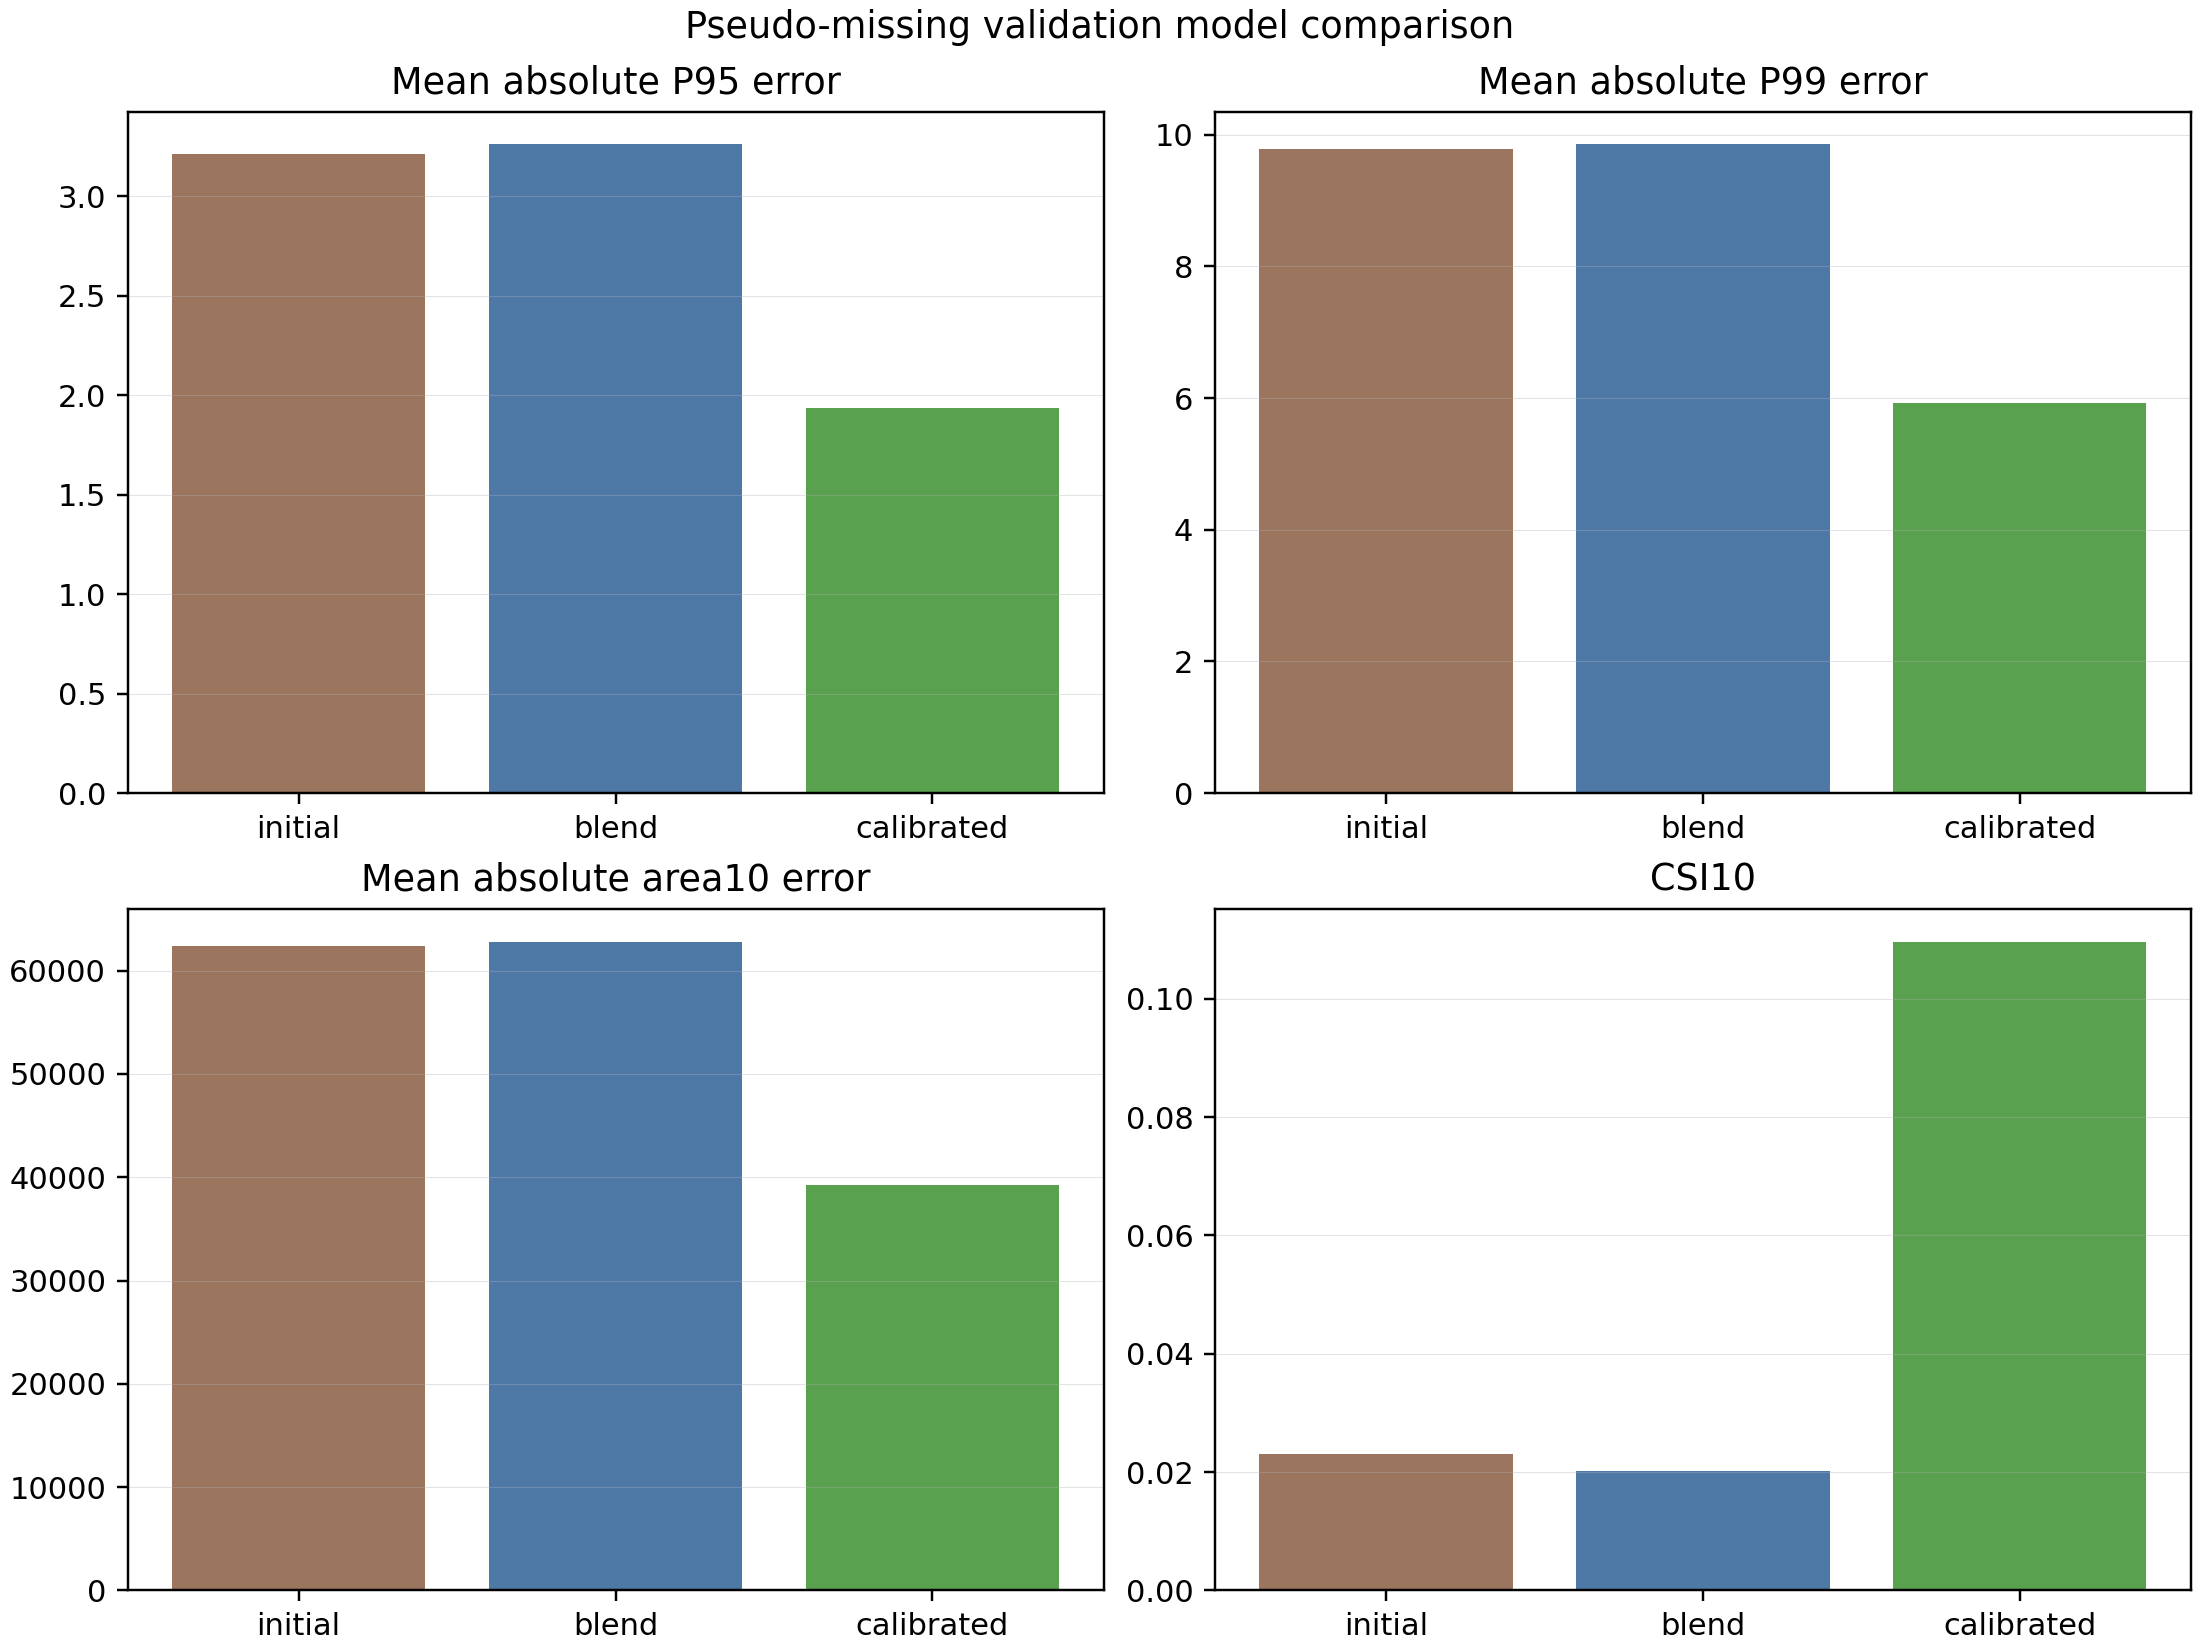
\includegraphics[width=0.85\textwidth]{outputs/figures/problem2_env/problem2_final_validation_model_comparison.png}
\caption{完成环境变量消融后伪缺失验证中不同模型版本的极端降水评价指标对比}
\label{fig:p2_validation_comparison}
\end{figure}

\subsubsection{环境变量消融检验}

为进一步判断新增环境变量是否适合直接纳入问题二相似检索，本文在伪缺失验证框架下比较 Base-old、Env-full 和 Env-key 三组环境距离设置，结果如表\ref{tab:p2_env_ablation}所示。

\begin{table}[H]
\centering
\caption{环境变量消融验证结果}
\label{tab:p2_env_ablation}
\resizebox{\textwidth}{!}{
\begin{tabular}{lcccccccccc}
\toprule
环境设置 & RMSE & MAE & Corr & P95误差 & P99误差 & Rmax误差 & $A_{10}$误差 & $A_{20}$误差 & CSI10 & F1\_10 \\
\midrule
Base-old & 2.6815 & 0.9607 & 0.3531 & 1.9351 & 5.9228 & 19.0788 & 39214.4 & 16833.6 & 0.1097 & 0.1773 \\
Env-full & 2.6923 & 0.9637 & 0.3537 & 1.9763 & 6.0206 & 18.8179 & 38861.9 & 16856.1 & 0.1084 & 0.1762 \\
Env-key & 2.6808 & 0.9614 & 0.3528 & 1.9507 & 6.0195 & 18.9924 & 39101.6 & 16950.8 & 0.1094 & 0.1777 \\
\bottomrule
\end{tabular}}
\end{table}

由表\ref{tab:p2_env_ablation}可见，三组环境距离设置的整体差异较小。Env-key 在 RMSE 和 F1\_10 上略优，Env-full 在 Rmax 误差和 $A_{10}$ 误差上略有改善，但二者在 P95、P99、$A_{20}$ 或空间相关系数上均未形成一致优势。Base-old 在 P95、P99、$A_{20}$、CSI10 等极端降水恢复指标上保持较稳定表现。考虑到问题二的目标是生成 KONG-REY 和 MAN-YI 的稳定可能降水场，而非单一指标最优，本文最终采用 Base-old 作为问题二相似检索中的环境距离设置。

这并不否定新增环境变量的物理意义。问题一结果表明 $landfrac\_500km$ 和 $terrain\_std\_300km$ 对降水结构具有非线性解释力；但在问题二有限样本相似检索中，过多环境变量可能提高匹配维度并稀释强度、路径和移动特征的主导作用。因此，本文将新增环境变量主要用于问题一机理解释和第三问虚拟路径情景下的环境重算，而不强行纳入最终问题二生成模型。

\subsubsection{关键参数敏感性分析}

前文模型中包含若干经验性超参数，包括 Top-$K$ 相似样本数量、相似距离各分量权重以及 EOF/PCA 融合系数 $\beta$。为检验参数设置对生成结果的影响，本文基于历史台风伪缺失验证框架进一步开展关键参数敏感性分析。为保证不同设置之间可比，选取与伪缺失验证一致的 $8$ 个历史验证事件，每个事件抽取 $60$ 个半小时时次，共 $480$ 个有效验证时次。每组参数均重新执行相似检索、模板迁移、EOF/PCA 融合和极端分位数校准，并统计 calibrated 版本与真实 GPM 降水场之间的误差。

敏感性分析的参数设置如表 \ref{tab:p2_sensitivity_setting} 所示。其中基准设置为 $K=20$、强度权重 $1.5$、移动权重 $1.2$、环境权重 $1.2$、EOF/PCA 融合系数 $\beta=0.3$。S1 与 S2 分别用于检验相似样本数量减少和增加时的影响；S3--S5 用于检验主要距离权重扰动；S6 与 S7 用于检验 EOF/PCA 融合强度变化。

\begin{table}[H]
\centering
\caption{相似检索与结构融合参数敏感性设置}
\label{tab:p2_sensitivity_setting}
\resizebox{\textwidth}{!}{
\begin{tabular}{lcccccc}
\toprule
设置 & $K$ & 强度权重 & 移动权重 & 环境权重 & EOF融合系数$\beta$ & 目的 \\
\midrule
基准 & 20 & 1.5 & 1.2 & 1.2 & 0.3 & 当前模型设定 \\
S1 & 10 & 1.5 & 1.2 & 1.2 & 0.3 & 检验较少相似样本时的稳定性 \\
S2 & 30 & 1.5 & 1.2 & 1.2 & 0.3 & 检验更多相似样本是否引入噪声 \\
S3 & 20 & 1.2 & 1.2 & 1.2 & 0.3 & 检验强度权重下降的影响 \\
S4 & 20 & 1.5 & 1.5 & 1.2 & 0.3 & 检验移动特征权重上升的影响 \\
S5 & 20 & 1.5 & 1.2 & 1.5 & 0.3 & 检验海陆环境权重上升的影响 \\
S6 & 20 & 1.5 & 1.2 & 1.2 & 0.0 & 不使用 EOF/PCA 融合 \\
S7 & 20 & 1.5 & 1.2 & 1.2 & 0.5 & 提高 EOF/PCA 融合强度 \\
\bottomrule
\end{tabular}}
\end{table}

各参数设置下的主要验证指标如表 \ref{tab:p2_sensitivity_result} 所示。总体来看，不同参数设置下 P95 误差、P99 误差、强降水面积误差和 CSI10 均未出现突变，说明本文生成模型对关键超参数具有一定鲁棒性。

\begin{table}[H]
\centering
\caption{关键参数敏感性分析结果}
\label{tab:p2_sensitivity_result}
\resizebox{\textwidth}{!}{
\begin{tabular}{lccccccccc}
\toprule
设置 & RMSE & MAE & Corr & P95误差 & P99误差 & Rmax误差 & $A_{10}$误差 & CSI10 & F1\_10 \\
\midrule
基准 & 2.7355 & 0.9749 & 0.3614 & 1.9761 & 6.1577 & 19.7977 & 40352.9 & 0.1160 & 0.1867 \\
S1 & 2.8055 & 0.9977 & 0.3371 & 2.0271 & 5.7534 & 15.5196 & 40074.8 & 0.1108 & 0.1791 \\
S2 & 2.7219 & 0.9706 & 0.3658 & 1.9990 & 6.3977 & 21.6752 & 40733.1 & 0.1153 & 0.1857 \\
S3 & 2.7313 & 0.9746 & 0.3606 & 1.9817 & 6.1744 & 19.8931 & 40318.8 & 0.1157 & 0.1861 \\
S4 & 2.7328 & 0.9739 & 0.3630 & 1.9779 & 6.1738 & 19.7450 & 40338.3 & 0.1161 & 0.1866 \\
S5 & 2.7334 & 0.9744 & 0.3614 & 1.9887 & 6.1668 & 19.7821 & 40237.7 & 0.1153 & 0.1858 \\
S6 & 2.7620 & 0.9881 & 0.3492 & 1.9588 & 6.0119 & 17.8568 & 40232.9 & 0.1133 & 0.1830 \\
S7 & 2.7276 & 0.9687 & 0.3677 & 1.9967 & 6.2303 & 21.2688 & 40552.9 & 0.1176 & 0.1888 \\
\bottomrule
\end{tabular}}
\end{table}

由表 \ref{tab:p2_sensitivity_result} 可见，当 $K$ 从 $20$ 调整为 $10$ 或 $30$ 时，模型性能整体保持稳定。$K=10$ 时，P99 误差和 Rmax 误差有所下降，但 Corr 和 CSI10 略低于基准，说明较少相似样本可能更容易突出局地极端值，但也更容易受个别历史样本影响，空间结构稳定性略弱。$K=30$ 时，Corr 略有提高，但 P99 和 Rmax 误差增大，说明引入更多相似性较弱的历史样本可能平滑或扰动极端结构。因此，本文取 $K=20$，在历史模板多样性和样本相似性之间取得折中。

当强度权重由 $1.5$ 降至 $1.2$ 时，P95、P99 与 Rmax 误差均较基准略有增大或基本持平，说明强度变量对极端降水刻画具有必要作用，这与问题一中强度变量对 $R_{95}$、$R_{99}$ 和强降水面积影响稳定的结论一致。提高移动权重至 $1.5$ 后，Corr 略有提升，P95 误差基本不变，说明移动速度和移动方向主要影响雨带空间结构，而非单独决定极端强度。提高环境权重至 $1.5$ 后，强降水面积误差略有下降，但 CSI10 略降，说明近岸和海陆环境变量对强降水范围具有一定调制作用，但过高权重可能使样本匹配过度偏向地理环境相似性。

对 EOF/PCA 融合系数的敏感性结果显示，$\beta=0$ 时模型不使用 EOF/PCA 结构修正，P95、P99 与 Rmax 误差略低，但 Corr 和 CSI10 低于基准；$\beta=0.5$ 时 Corr、CSI10 和 F1\_10 略高，但 Rmax 误差有所增大。说明 EOF/PCA 融合可以提高大尺度结构稳定性和强降水识别能力，但过强的 EOF 约束可能进一步平滑局地极端峰值。综合极端误差、空间相关和强降水识别指标，$\beta=0.3$ 能在大尺度结构稳定性和局地极端保留之间取得较好平衡，因此作为本文最终设置。

综上，关键参数扰动下模型评价指标未发生方向性突变，表明本文相似检索--模板迁移--EOF/PCA 修正--极端校准的生成链条具有较好的参数鲁棒性。基准设置下虽然并非每一项指标均达到最优，但在 P95/P99 极端误差、强降水面积误差、CSI10 和空间相关性之间取得了较均衡的表现，适合作为后续 KONG-REY 与 MAN-YI 可能降水分布生成的最终参数组合。

\begin{figure}[H]
\centering
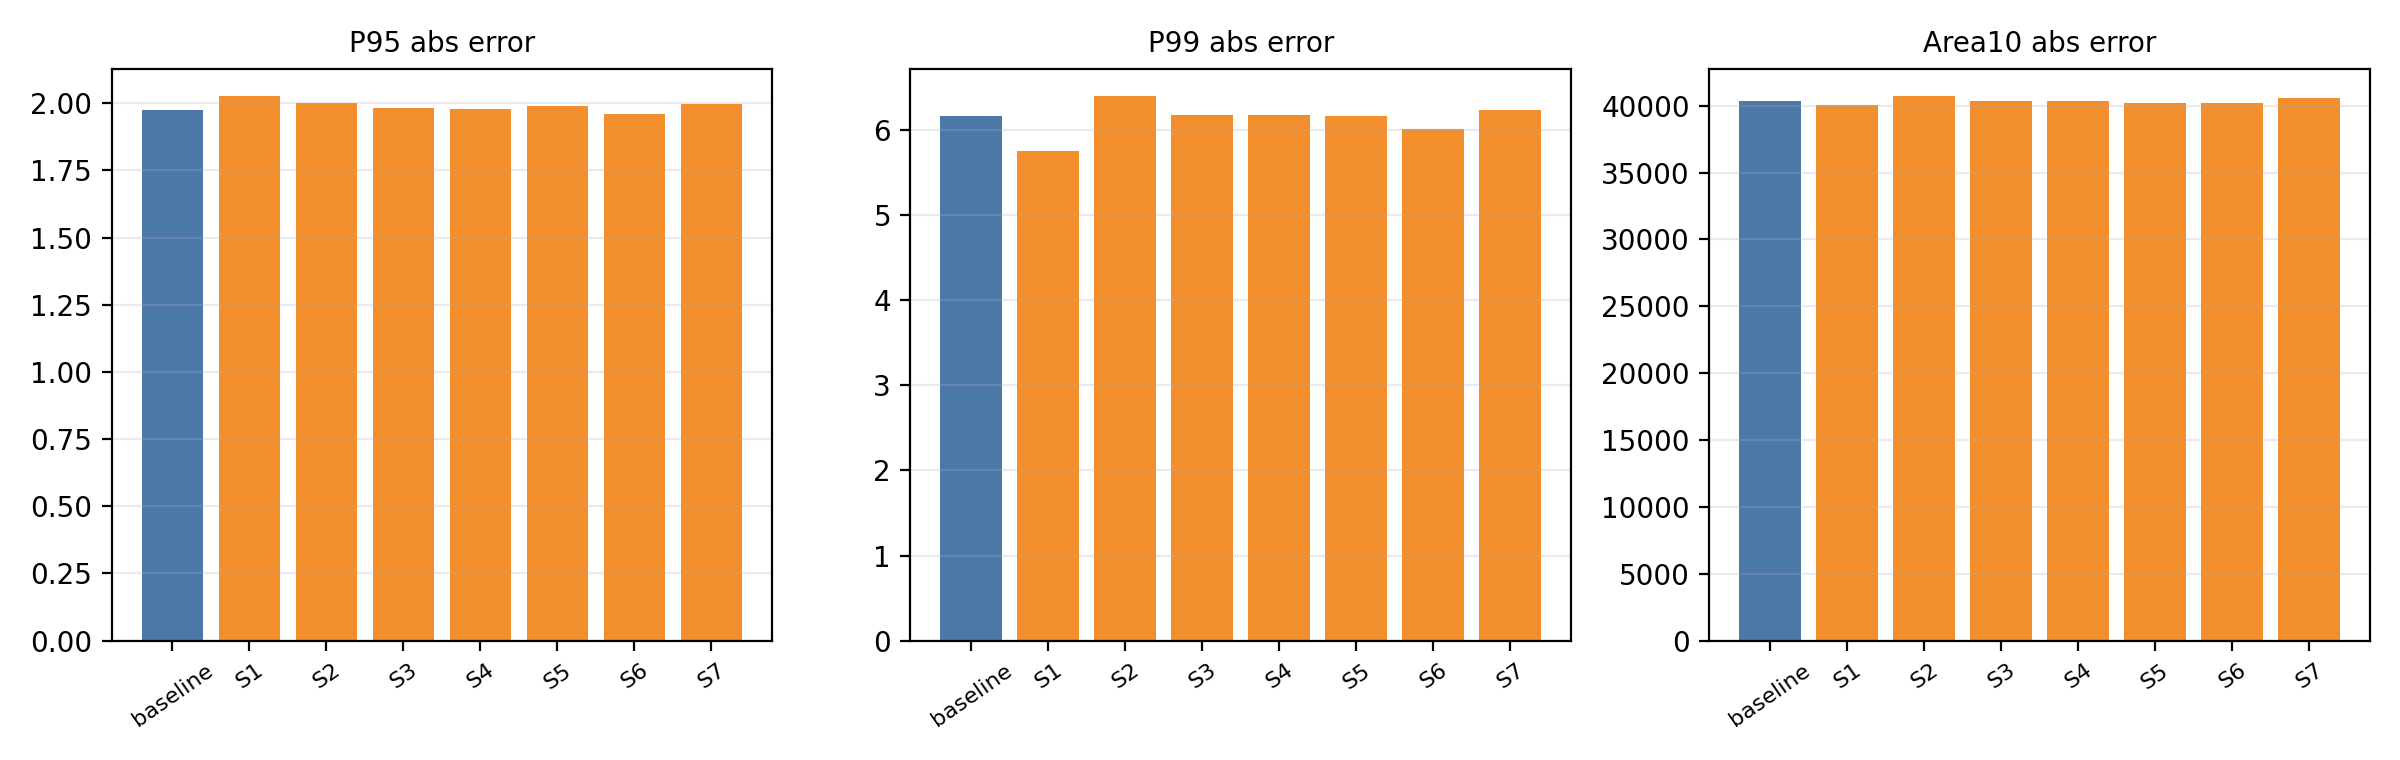
\includegraphics[width=0.9\textwidth]{outputs/figures/problem2_sensitivity_analysis/sensitivity_bar_extreme_errors.png}
\caption{不同参数设置下极端降水误差对比}
\label{fig:p2_sensitivity_extreme}
\end{figure}

\begin{figure}[H]
\centering
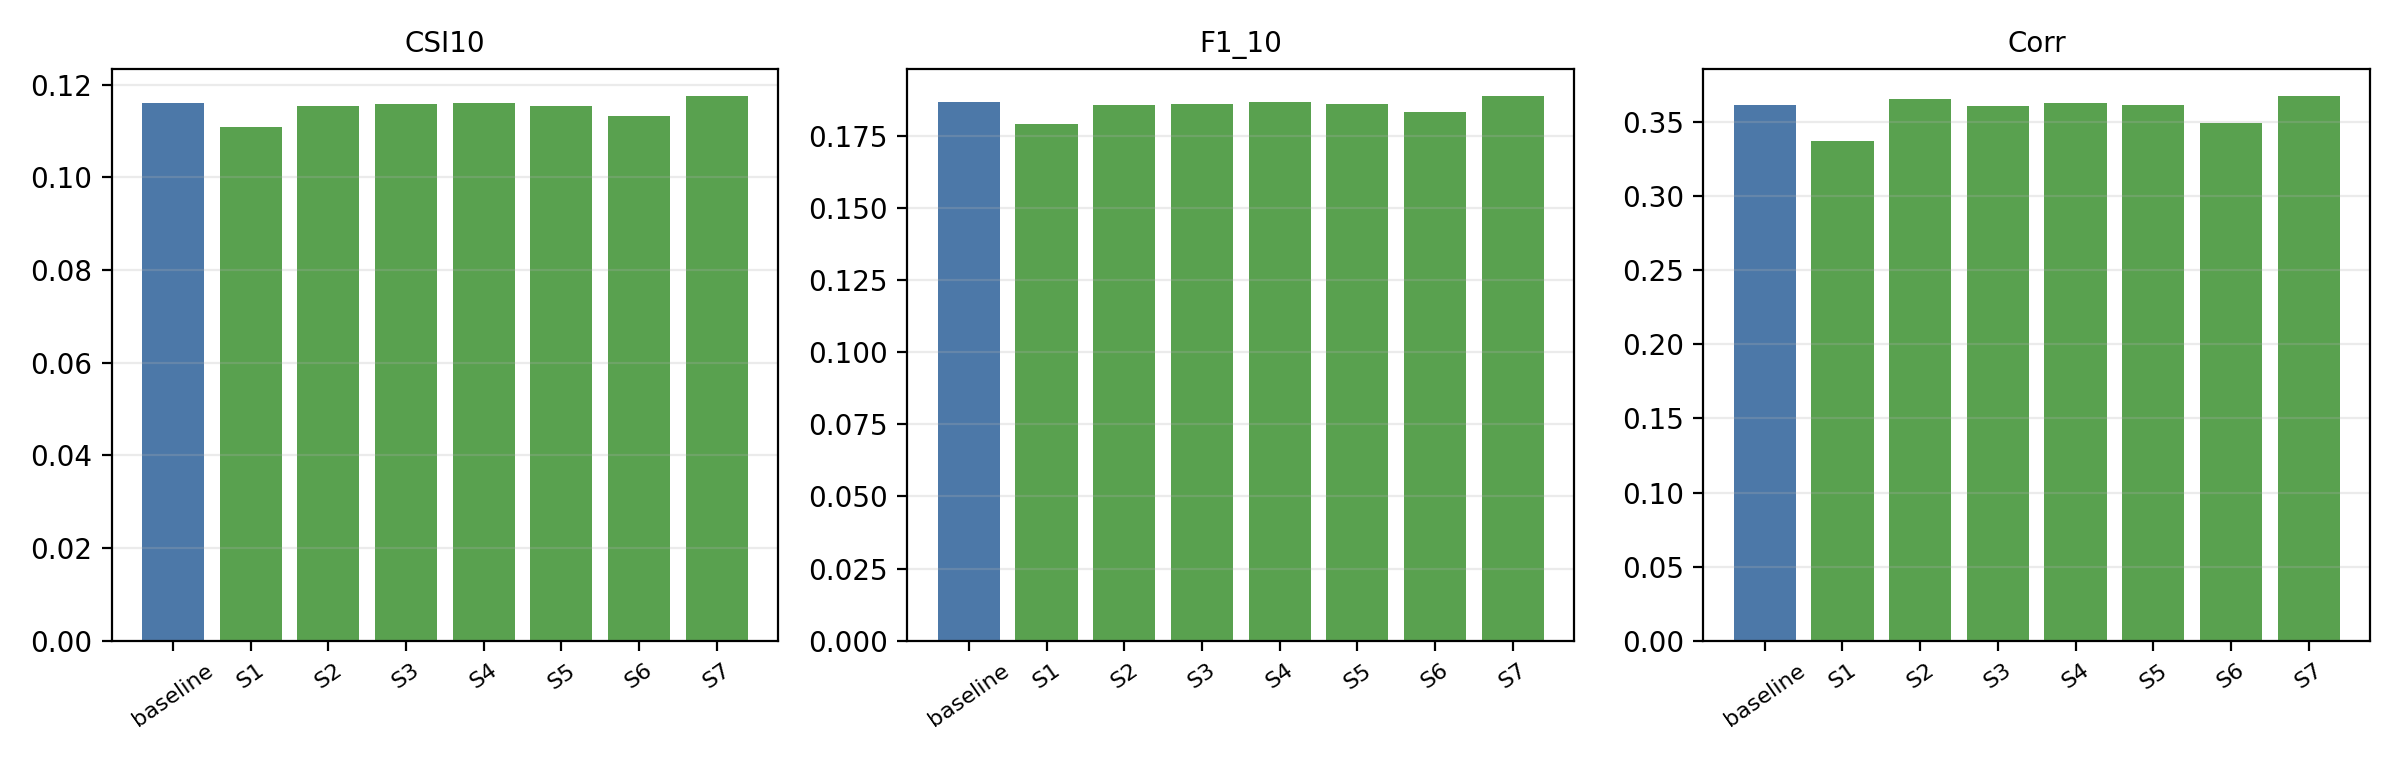
\includegraphics[width=0.9\textwidth]{outputs/figures/problem2_sensitivity_analysis/sensitivity_bar_skill_scores.png}
\caption{不同参数设置下空间相关与强降水识别指标对比}
\label{fig:p2_sensitivity_skill}
\end{figure}

\subsection{KONG-REY 与 MAN-YI 生成结果分析}

\subsubsection{最终结果说明}

基于 6.5 节得到的极端分位数校准场，本文得到 KONG-REY 和 MAN-YI 的最终半小时可能降水分布。需要强调的是，本结果为基于历史相似台风、路径强度条件和海陆环境生成的可能降水场，不是 GPM 真实观测。

表 \ref{tab:p2_final_summary_a} 和表 \ref{tab:p2_final_summary_b} 给出了两场台风的最终生成结果摘要。其中，表 \ref{tab:p2_final_summary_a} 侧重目标台风过程与 storm-relative 结构指标，表 \ref{tab:p2_final_summary_b} 侧重固定经纬度网格上的真实地理落区指标，从而区分降水结构随台风移动反复维持的持续性和真实地理位置经历强降水的累计时长。

\begingroup
\renewcommand{\thetable}{\thesection.\arabic{table}A}
\renewcommand{\theHtable}{\thetable}
\begin{table}[H]
\centering
\caption{目标台风过程与 storm-relative 结构指标（最终 Base-old 生成）}
\label{tab:p2_final_summary}
\label{tab:p2_final_summary_a}
\small
\setlength{\tabcolsep}{3pt}
\resizebox{\textwidth}{!}{
\begin{tabular}{lrrrrrrrrrrrl}
\toprule
台风 
& \makecell{时次数}
& \makecell{WND最大值\\/(m/s)}
& \makecell{PRES最小值\\/hPa}
& \makecell{最大P95\\/(mm/h)}
& \makecell{最大P99\\/(mm/h)}
& \makecell{最大Rmax\\/(mm/h)}
& \makecell{最大$A_{10}$\\/km$^2$}
& \makecell{最大$A_{20}$\\/km$^2$}
& \makecell{相对坐标\\$D_{10}^{\max}$/h}
& \makecell{相对坐标\\$D_{20}^{\max}$/h}
& \makecell{总量代理\\/(mm$\cdot$km$^2$)}
& \makecell{主雨象限} \\
\midrule
KONG-REY 
& 421
& 60.0 
& 920.0 
& 3.8809 
& 16.8213 
& 53.7328 
& 87800.0 
& 30600.0 
& 146.0
& 112.5
& 492974958.99
& front\_left \\
MAN-YI 
& 553
& 62.0 
& 920.0 
& 4.9931 
& 17.1411 
& 54.4054 
& 115500.0 
& 29000.0 
& 196.0
& 98.5
& 686489406.31
& front\_left \\
\bottomrule
\end{tabular}}
\end{table}

\addtocounter{table}{-1}
\renewcommand{\thetable}{\thesection.\arabic{table}B}
\renewcommand{\theHtable}{\thetable}
\begin{table}[H]
\centering
\caption{真实地理坐标落区指标}
\label{tab:p2_final_summary_b}
\small
\setlength{\tabcolsep}{4pt}
\begin{tabularx}{\textwidth}{lcccc>{\raggedright\arraybackslash}X}
\toprule
台风
& \makecell{地理最大\\累计降水/mm}
& \makecell{地理\\$D_{10}^{\max}$/h}
& \makecell{$P_{\mathrm{geo}}\ge100$ mm\\面积/km$^2$}
& \makecell{$D_{10,\mathrm{geo}}\ge3$ h\\面积/km$^2$}
& 主要特征 \\
\midrule
KONG-REY
& 722.047
& 27.0
& $1.229\times 10^6$
& $8.055\times 10^5$
& \makecell[l]{局地累计峰值更高；\\固定地理单点持续时间略长} \\
MAN-YI
& 533.592
& 23.5
& $2.071\times 10^6$
& $1.307\times 10^6$
& \makecell[l]{累计雨区和持续强降水\\覆盖范围更广} \\
\bottomrule
\end{tabularx}
\end{table}
\endgroup

需要说明的是，表中“相对坐标$D_{10}^{\max}$”和“相对坐标$D_{20}^{\max}$”是在台风相对运动坐标系下统计得到的强降水持续结构指标，表示某一相对台风中心方位在台风生命史中反复处于强降水区的累计时长；“地理$D_{10}^{\max}$”则是在固定经纬度网格上统计得到的强降水持续时间，表示某一真实地理位置经历 $10\ \mathrm{mm/hr}$ 及以上强降水的累计时长。二者刻画对象不同，前者用于解释降水结构，后者用于刻画真实地理落区。

KONG-REY 的生成过程持续 $210.5$ h，共 $421$ 个半小时时次，最大风速为 $60.0$，最低气压为 $920.0$。其生成降水场中，最大格点雨强达到 $53.733\ \mathrm{mm/hr}$，发生于 2024-10-26 23:00:00；最大 P95 降水强度为 $3.881\ \mathrm{mm/hr}$，最大 P99 降水强度为 $16.821\ \mathrm{mm/hr}$，二者均发生于 2024-10-30 09:00:00；$10\ \mathrm{mm/hr}$ 以上强降水面积峰值为 $87800\ \mathrm{km^2}$，$20\ \mathrm{mm/hr}$ 以上强降水面积峰值为 $30600\ \mathrm{km^2}$。其累计降水体量代理值为 $4.930\times 10^8\ \mathrm{mm\cdot km^2}$，累计降水主导象限为移动方向左前侧。

MAN-YI 的生成过程持续 $276.5$ h，共 $553$ 个半小时时次，最大风速为 $62.0$，最低气压为 $920.0$。其最大格点雨强为 $54.405\ \mathrm{mm/hr}$，发生于 2024-11-14 10:30:00；最大 P95 为 $4.993\ \mathrm{mm/hr}$，发生于 2024-11-14 03:30:00；最大 P99 为 $17.141\ \mathrm{mm/hr}$，发生于 2024-11-14 04:30:00；$10\ \mathrm{mm/hr}$ 以上强降水面积峰值达到 $115500\ \mathrm{km^2}$，发生于 2024-11-14 04:00:00，$20\ \mathrm{mm/hr}$ 以上强降水面积峰值为 $29000\ \mathrm{km^2}$。其累计降水体量代理值为 $6.865\times 10^8\ \mathrm{mm\cdot km^2}$，累计降水主导象限同样为移动方向左前侧。

\subsubsection{两场台风对比}

从极端降水强度看，MAN-YI 的最大 P95、最大 P99 和最大格点雨强均略高于 KONG-REY；从空间范围看，MAN-YI 的 $10\ \mathrm{mm/hr}$ 强降水面积峰值为 $115500\ \mathrm{km^2}$，明显高于 KONG-REY 的 $87800\ \mathrm{km^2}$；从台风相对坐标下的结构持续性看，MAN-YI 的相对坐标 $D_{10}^{\max}$ 为 $196.0$ h，高于 KONG-REY 的 $146.0$ h，说明其强降水结构在相对台风中心方位上维持更久。固定经纬度落区上，KONG-REY 的地理 $D_{10}^{\max}$ 为 $27.0$ h，略高于 MAN-YI 的 $23.5$ h；但 MAN-YI 的 $P_{\mathrm{cum}}\ge100\ \mathrm{mm}$ 面积和 $D_{10}\ge3\ \mathrm{h}$ 面积均更大，表明其真实地理影响范围更广。

作为生成结果的形态诊断，本文进一步计算最终校准场的雨带横向等效带宽。KONG-REY 的平均 $B$ 为 $503.2\ \mathrm{km}$、最大 $B$ 为 $824.0\ \mathrm{km}$；MAN-YI 的平均 $B$ 为 $570.7\ \mathrm{km}$、最大 $B$ 为 $1439.2\ \mathrm{km}$。这说明在生成结果中，MAN-YI 不仅强降水面积更大，其主要降水带的横向铺展也更明显。该指标仅用于生成场诊断，不参与目标台风安全输入和相似检索。

\begin{figure}[htbp]
    \centering
    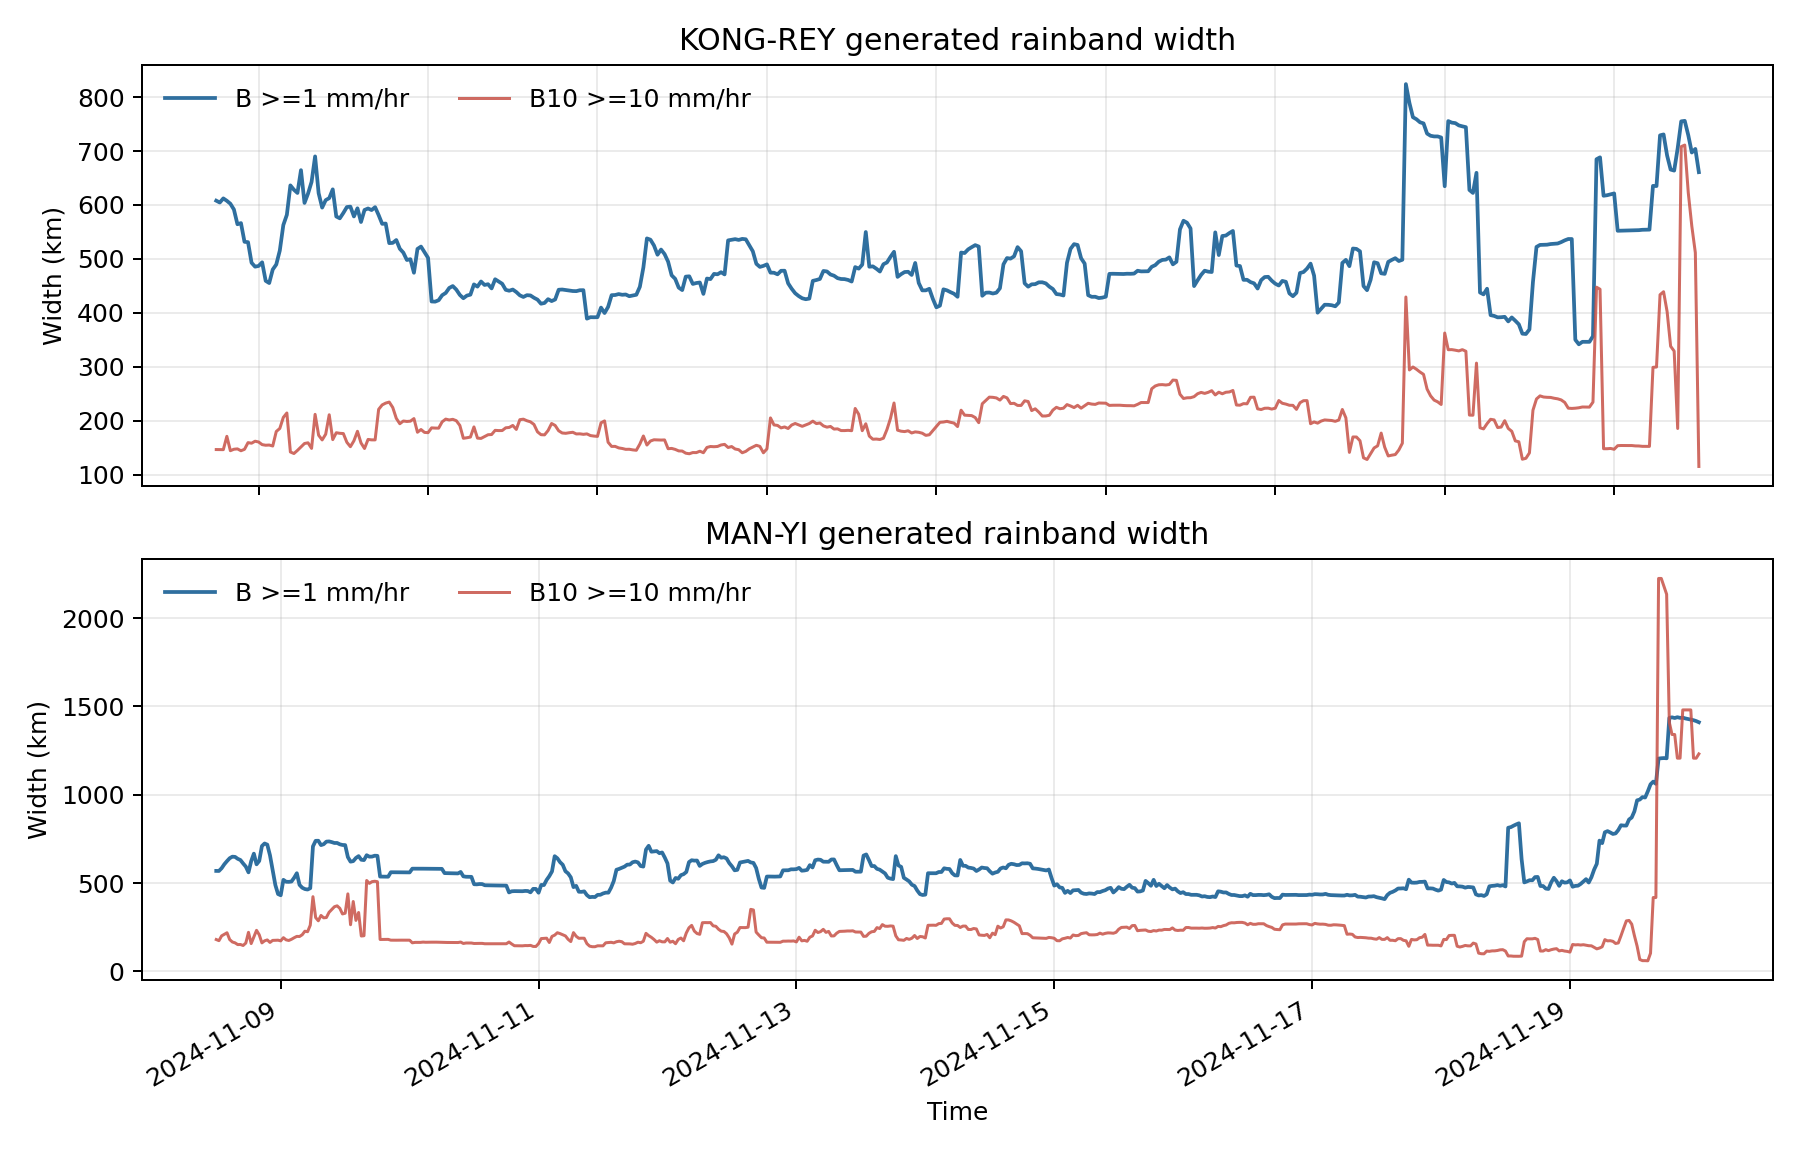
\includegraphics[width=0.90\textwidth]{outputs/figures/problem2_env/problem2_rainband_width_timeseries.png}
    \caption{KONG-REY 和 MAN-YI 生成雨带带宽随时间变化}
    \label{fig:problem2_rainband_width_timeseries}
\end{figure}

两场台风的累计降水主导象限均为移动方向左前侧（front\_left），说明生成结果保持了台风降水相对于移动方向的非对称结构特征。这与问题一中发现的台风降水质心偏移、移动方向和非对称雨带之间的关系一致。

\begin{figure}[H]
\centering
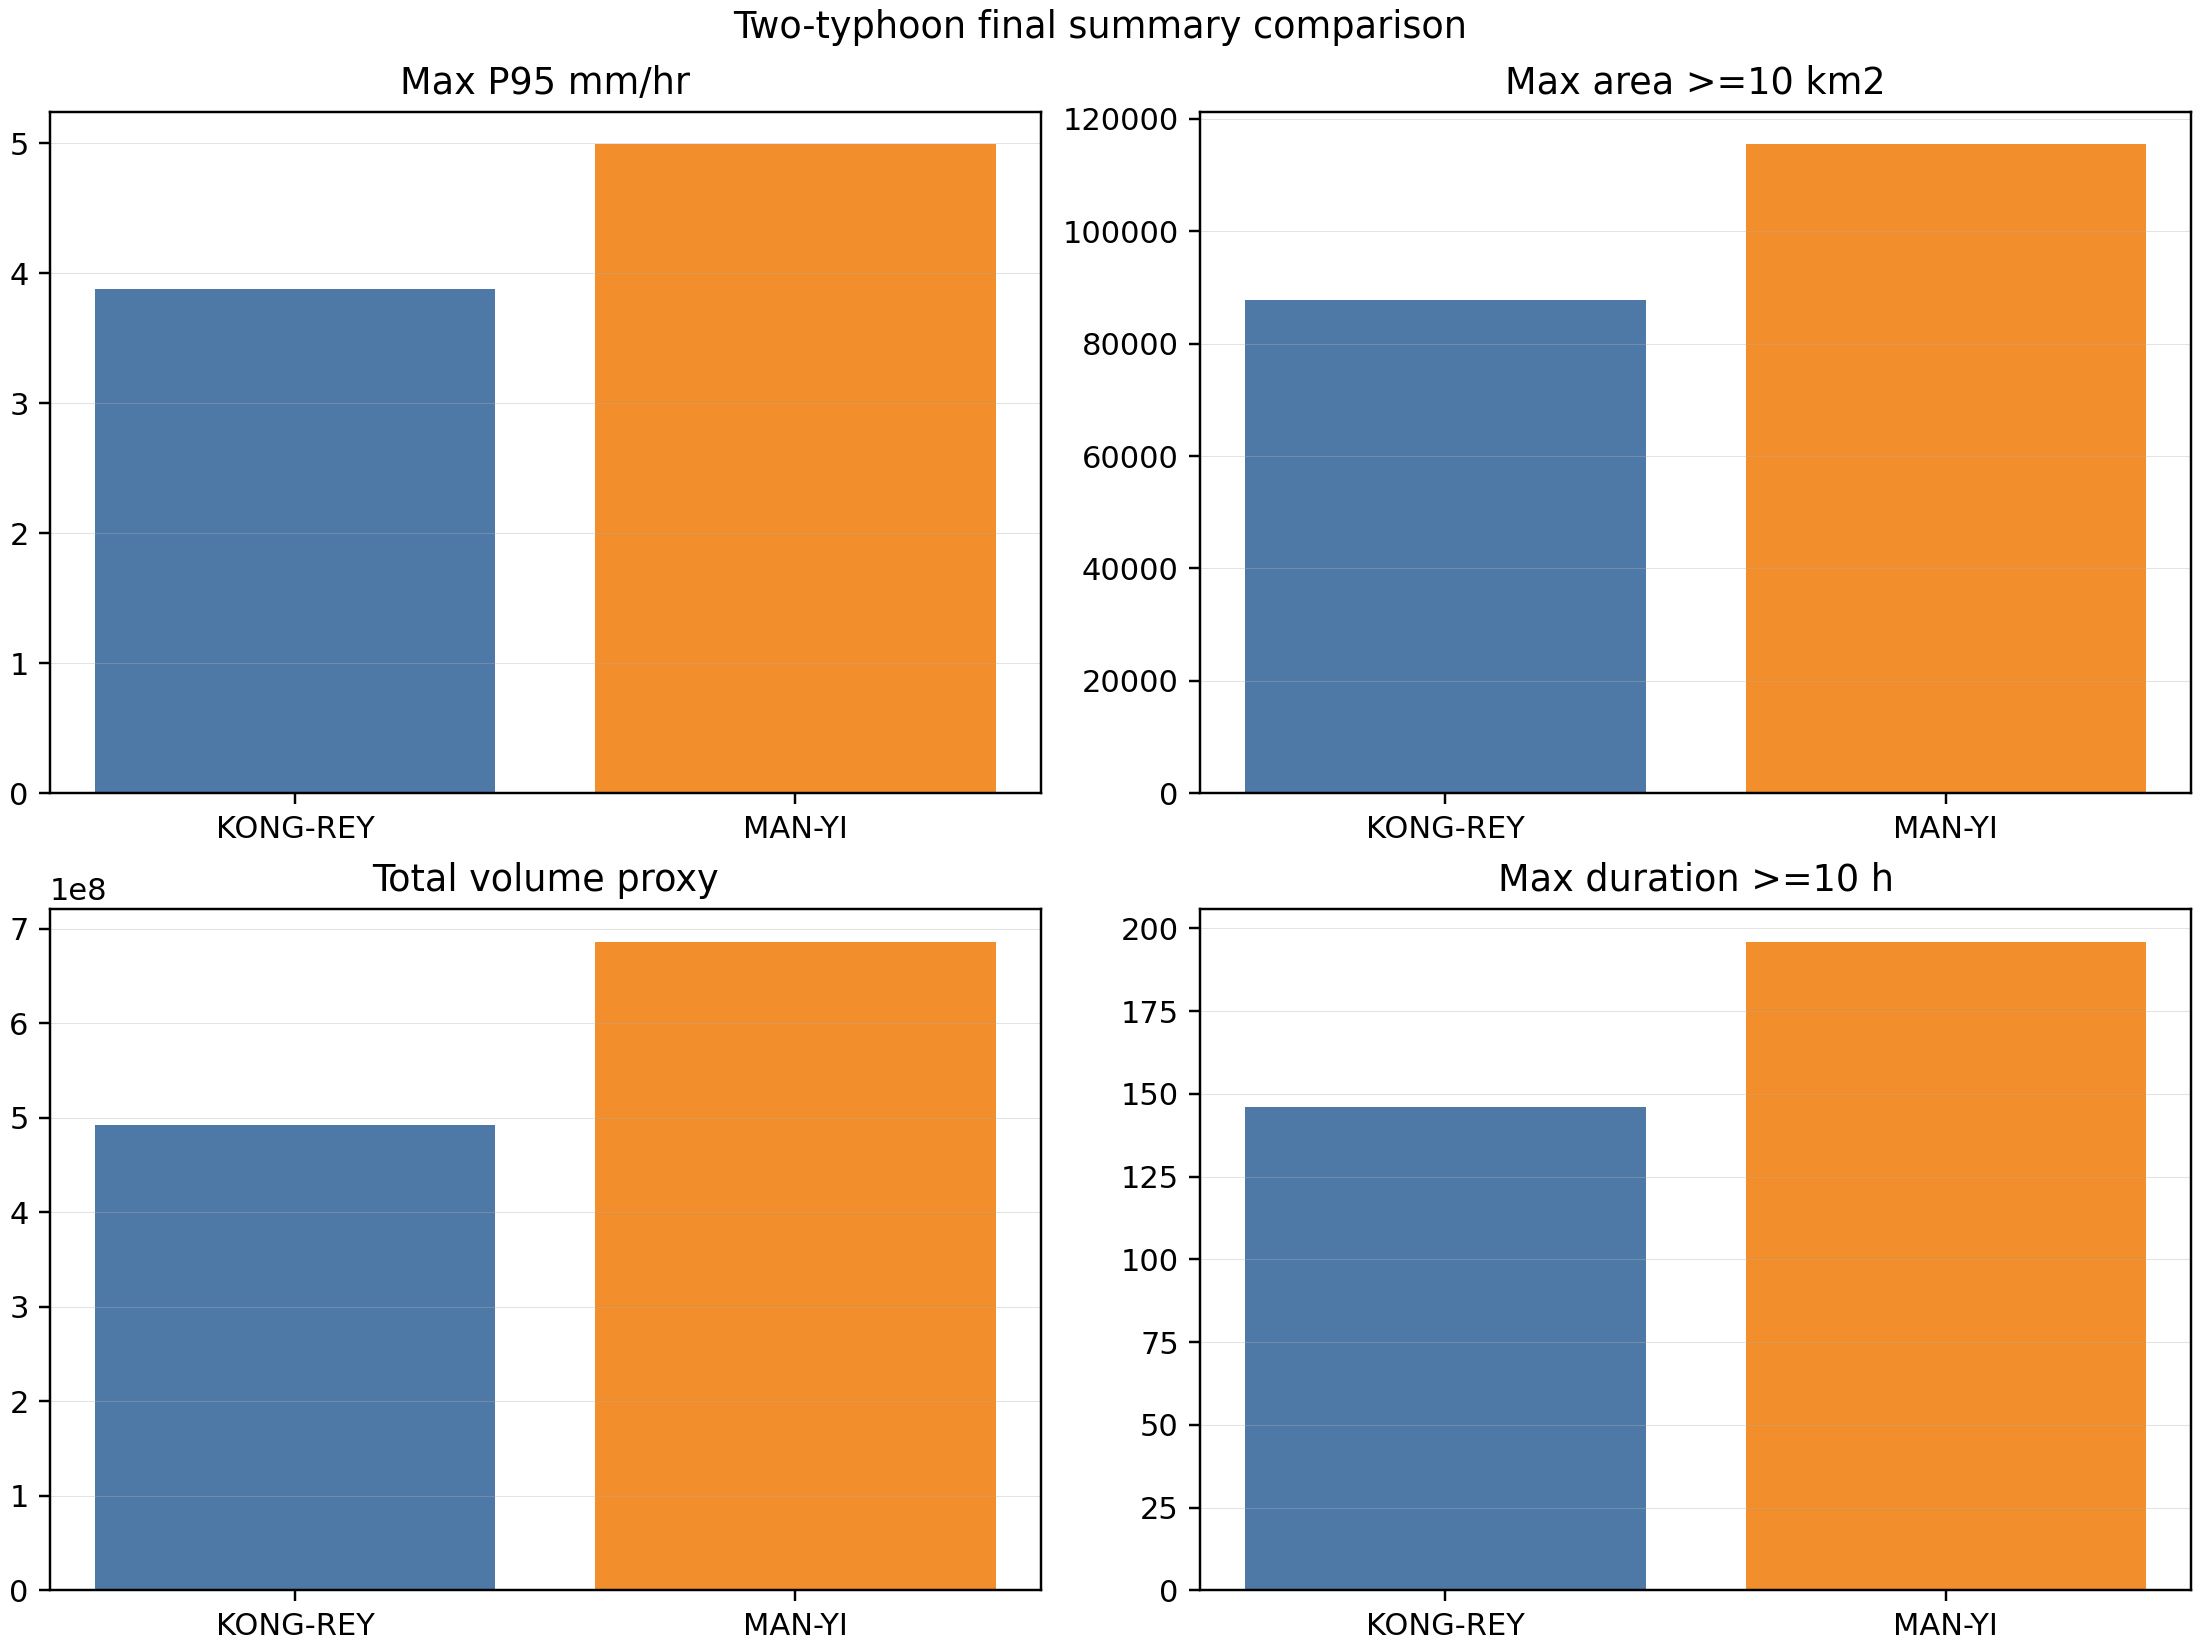
\includegraphics[width=0.95\textwidth]{outputs/figures/problem2_env/problem2_final_two_typhoons_summary_compare.png}
\caption{KONG-REY 与 MAN-YI 最终生成降水指标对比}
\label{fig:p2_two_typhoon_compare}
\end{figure}

\subsubsection{代表时刻降水场}

图 \ref{fig:p2_kongrey_fields} 和图 \ref{fig:p2_manyi_fields} 分别展示 KONG-REY 与 MAN-YI 的代表时刻台风相对坐标降水场。图中横轴为移动前方方向，纵轴为移动方向左侧。可以看出，两场台风在强度峰值和强降水面积峰值附近均形成较大范围的强降水区，且雨区相对于台风中心具有明显非对称性。

\begin{figure}[H]
\centering
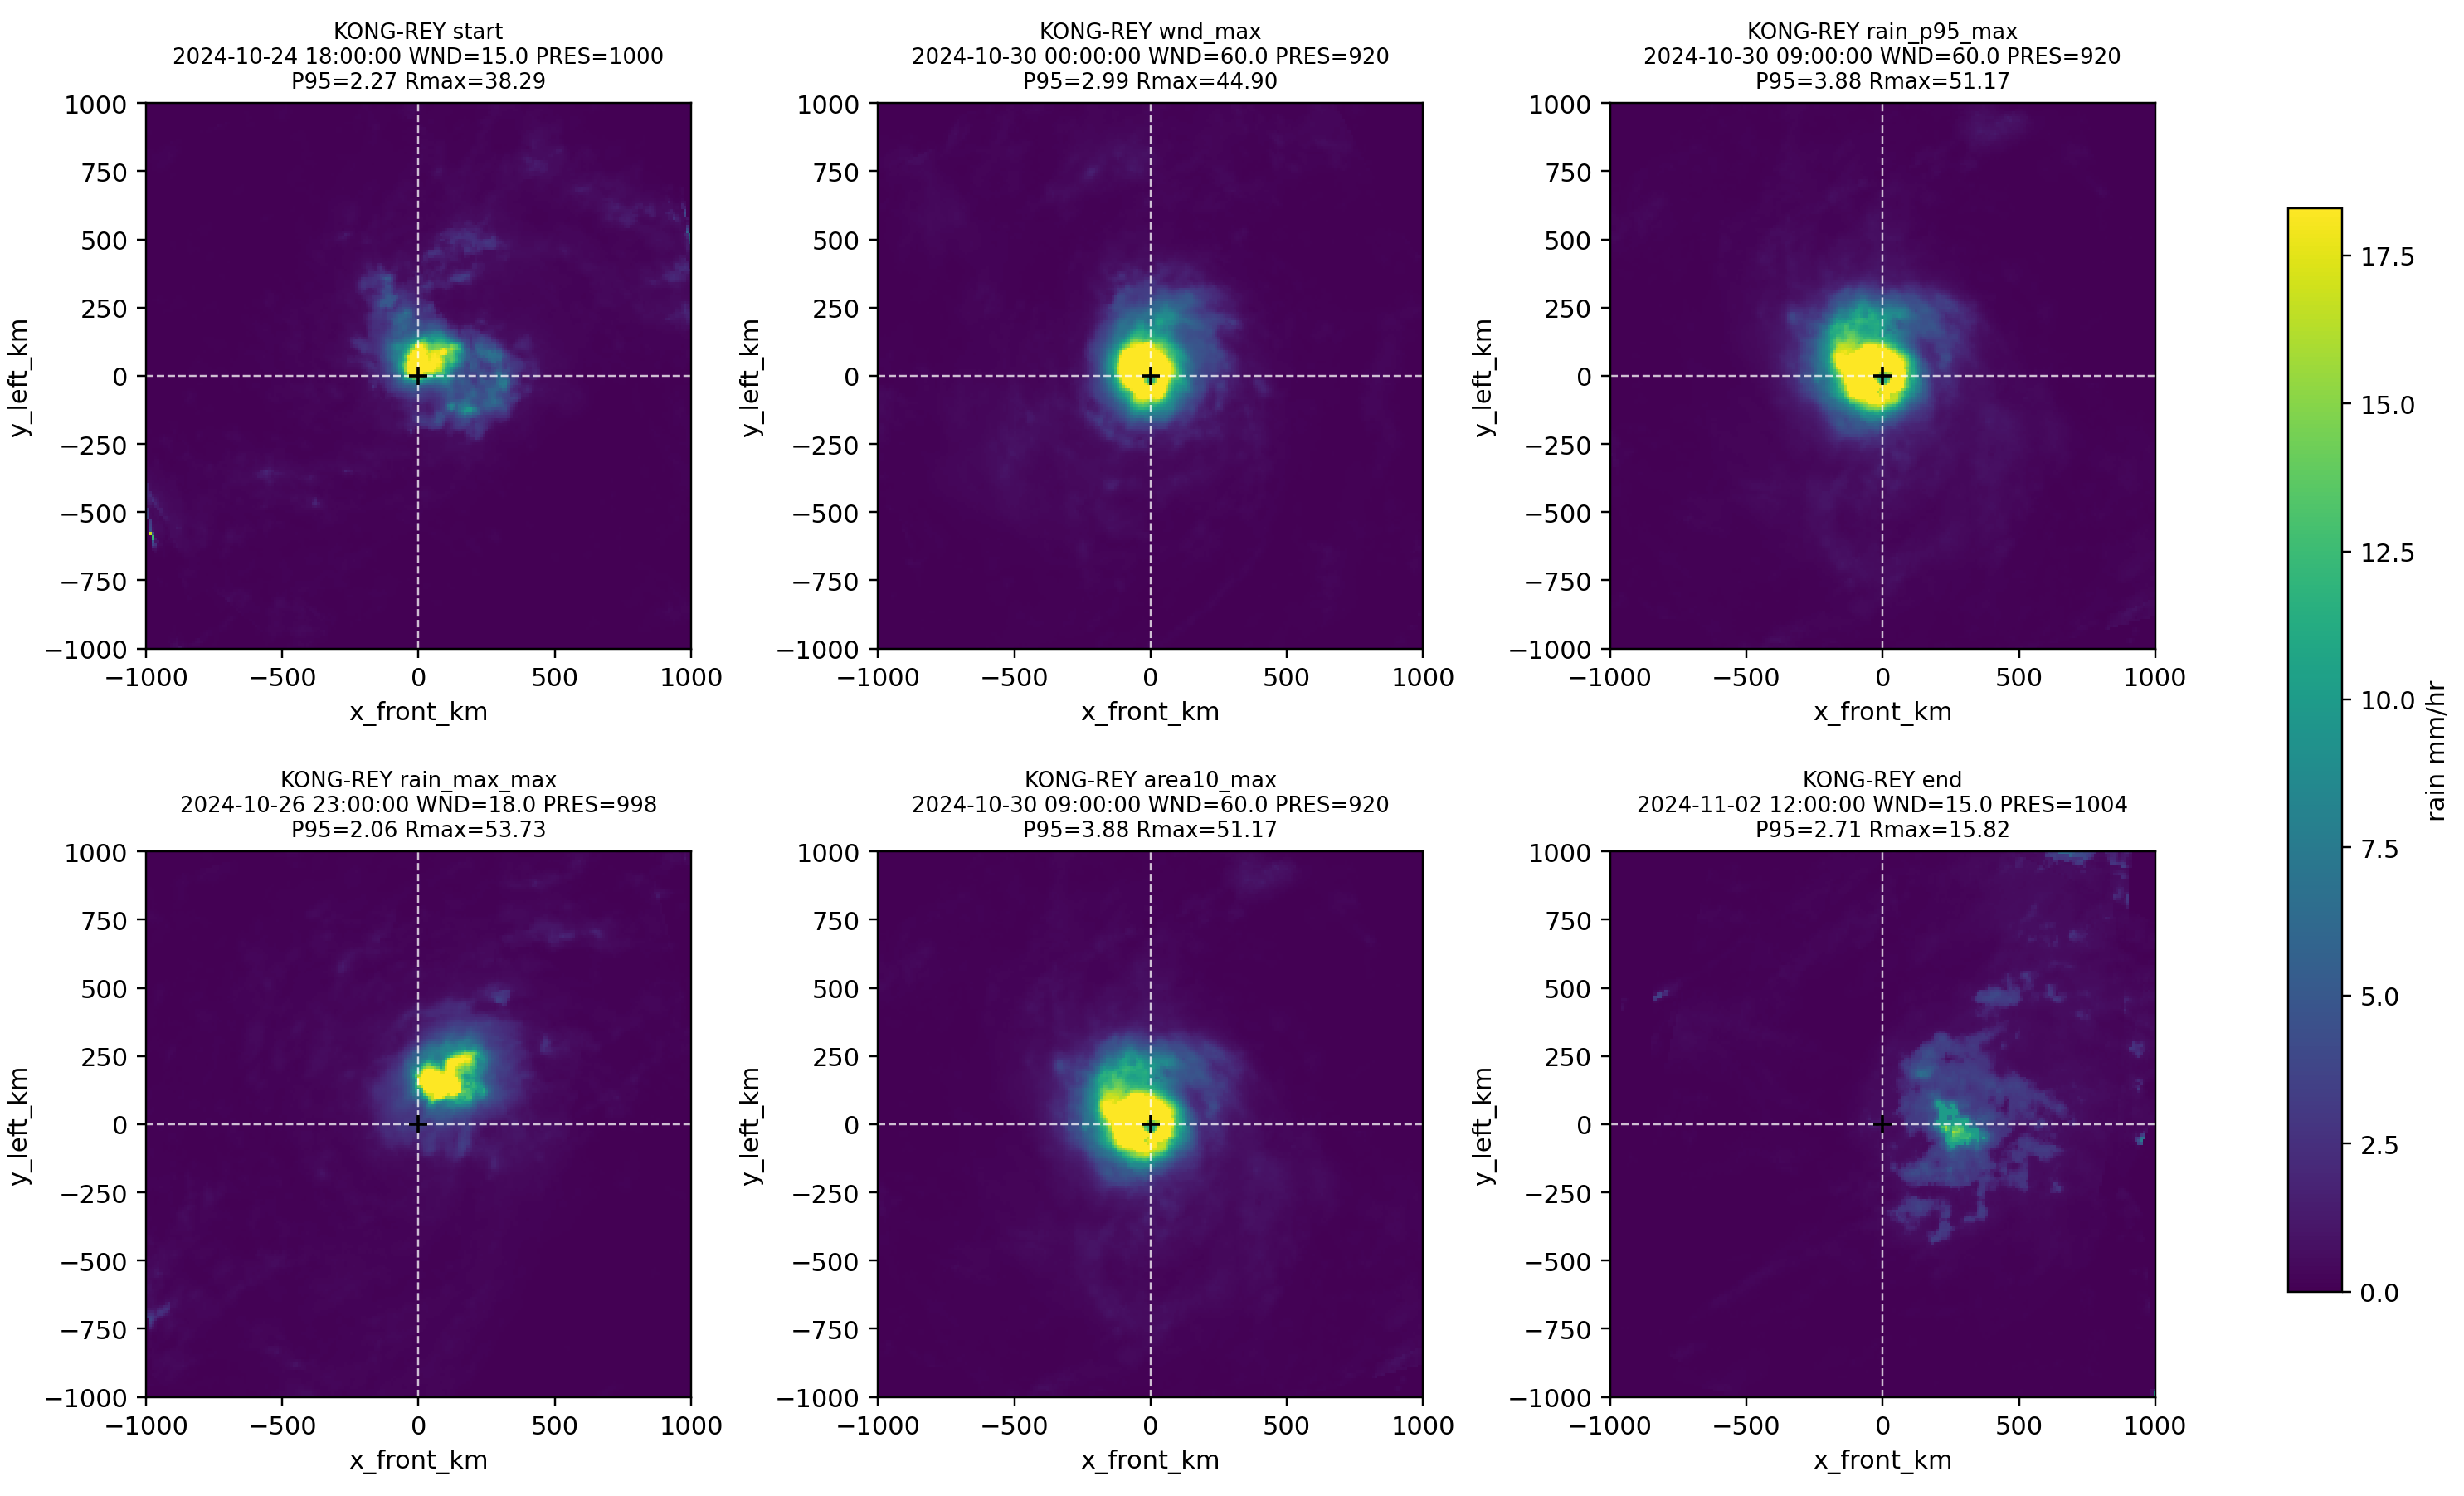
\includegraphics[width=0.95\textwidth]{outputs/figures/problem2_env/KONG_REY_final_representative_fields.png}
\caption{KONG-REY 代表时刻台风相对坐标降水场}
\label{fig:p2_kongrey_fields}
\end{figure}

\begin{figure}[H]
\centering
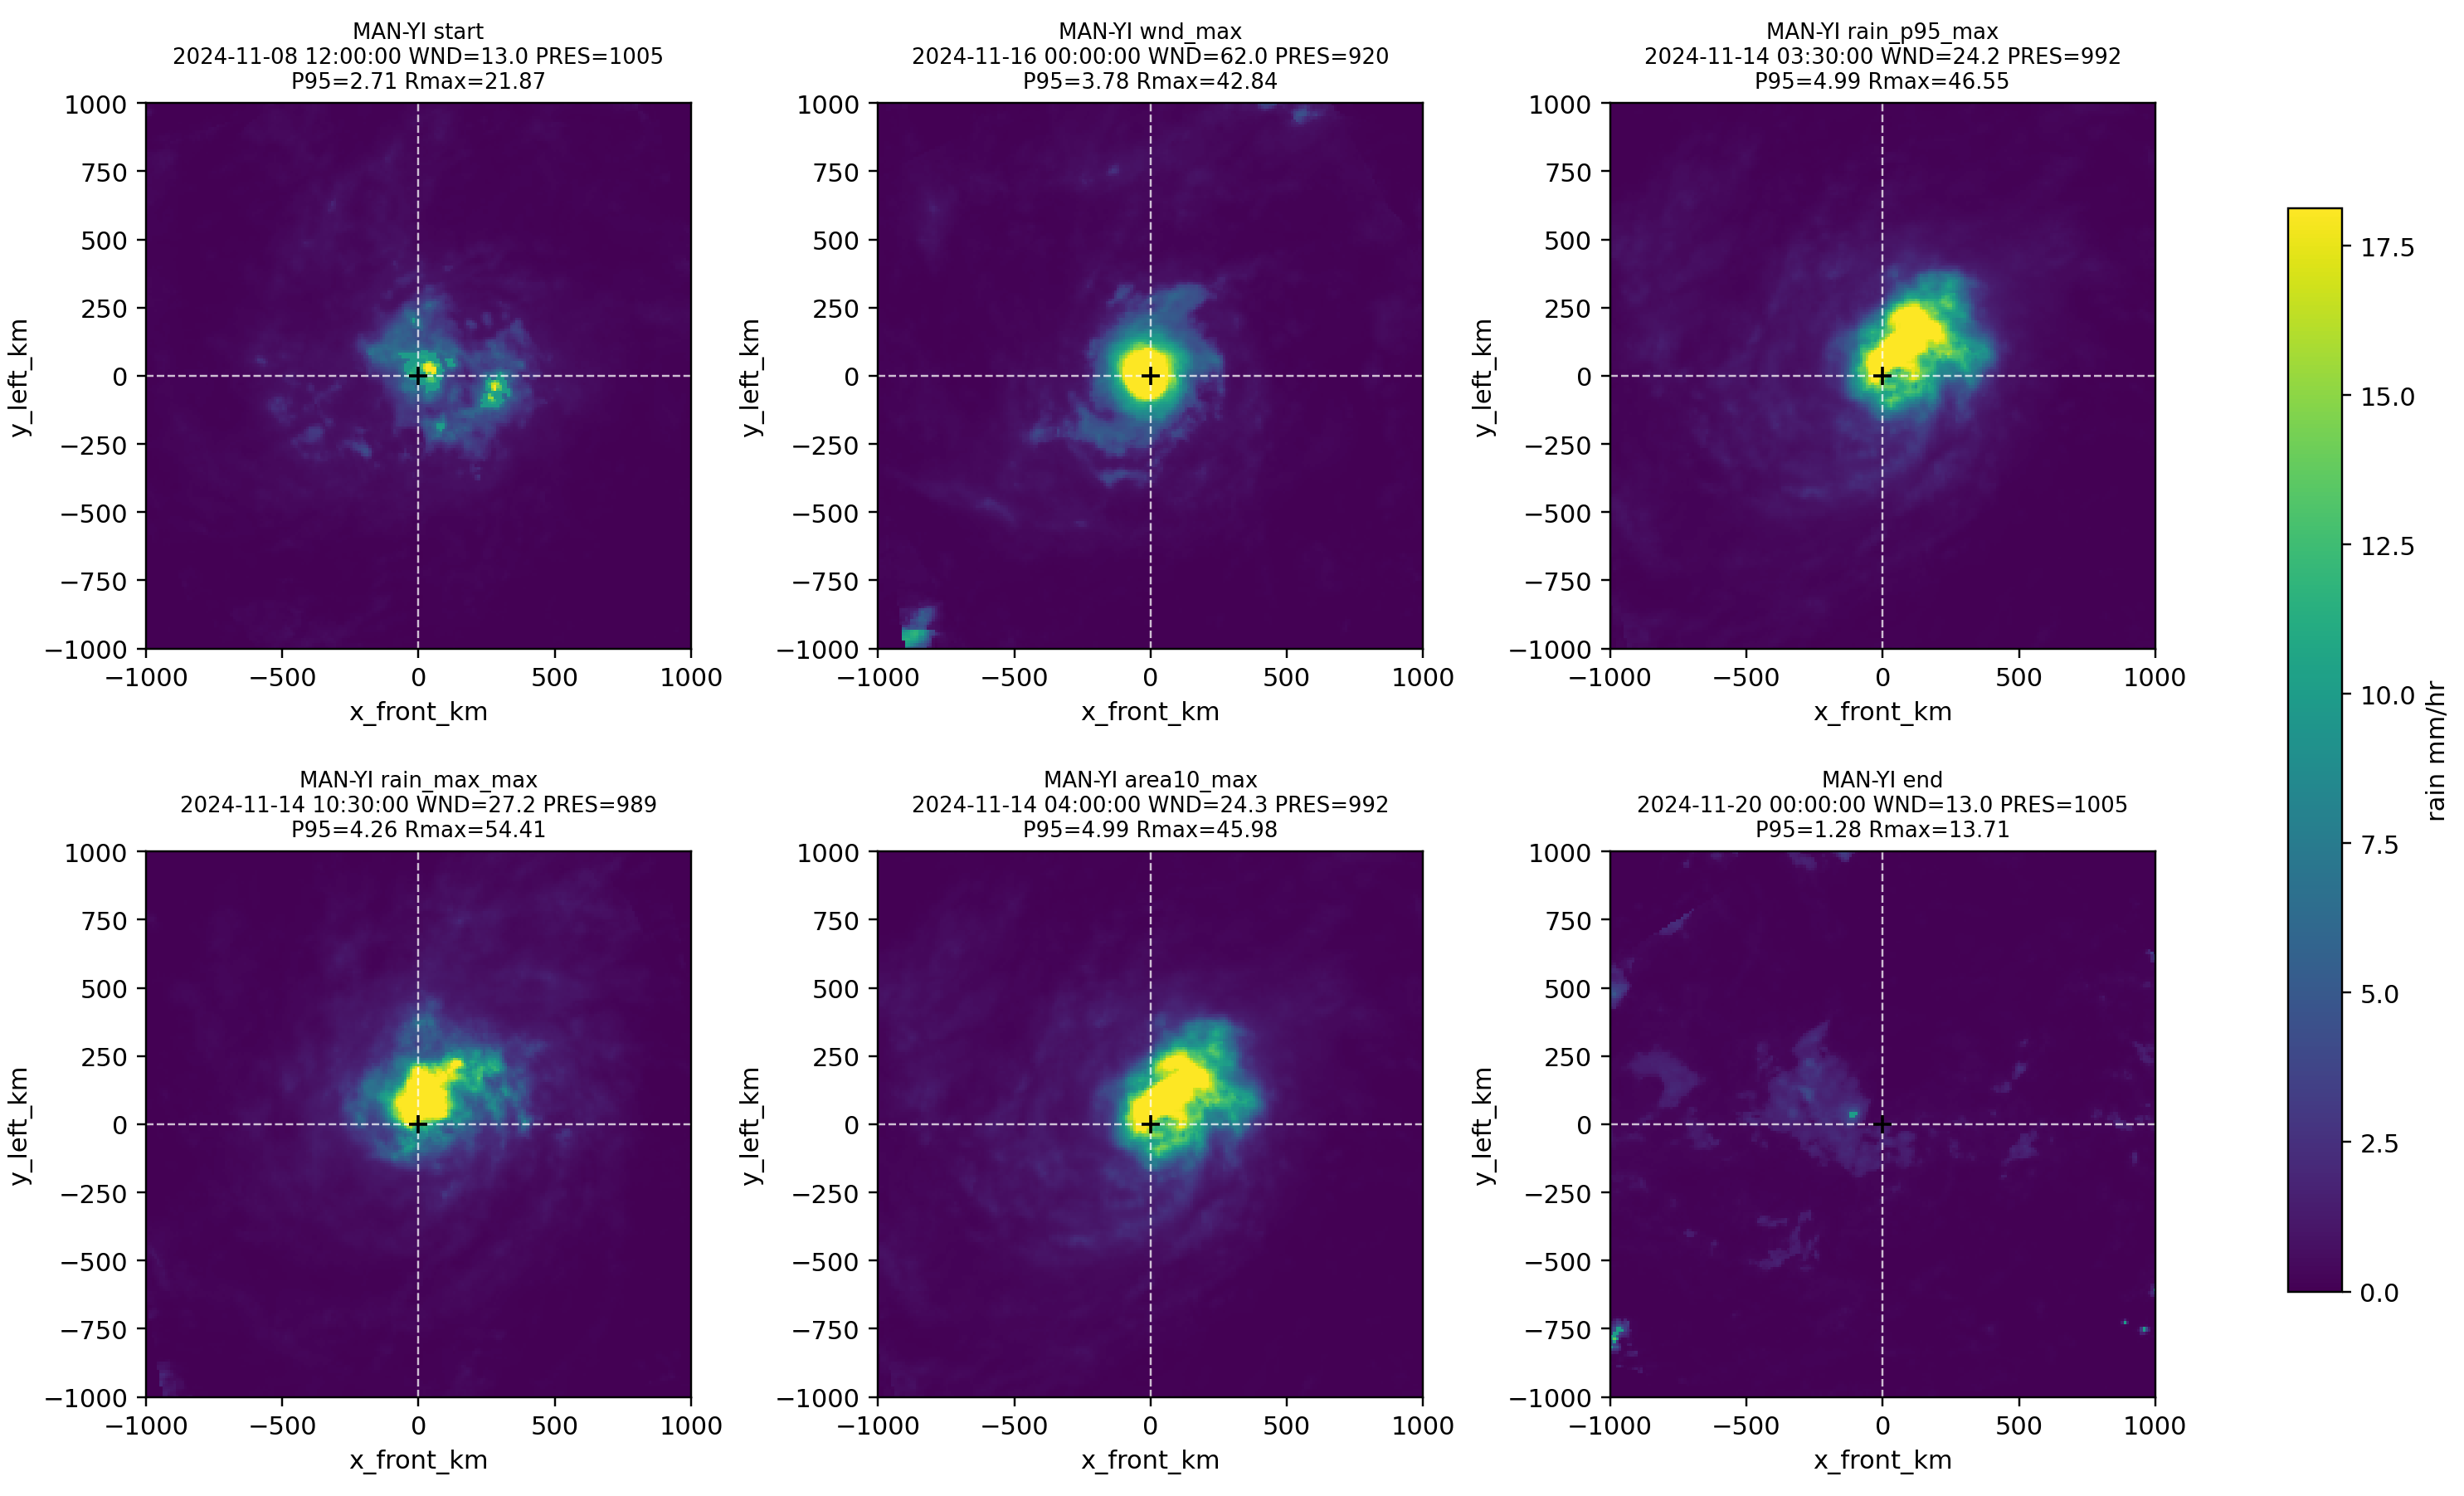
\includegraphics[width=0.95\textwidth]{outputs/figures/problem2_env/MAN_YI_final_representative_fields.png}
\caption{MAN-YI 代表时刻台风相对坐标降水场}
\label{fig:p2_manyi_fields}
\end{figure}

\subsubsection{累计降水、最大半小时降水与强降水持续时间}

本节给出的累计降水图、最大半小时降水图和强降水持续时间图均定位为 storm-relative 坐标下的结构解释图，而不是固定地理空间中的最终落区图。这些图是在台风相对运动坐标系下统计得到的，用于描述降水相对于台风中心及移动方向的结构特征，如主雨带位置、非对称性和持续性；它们不直接表示固定地理位置上的真实累计降水或持续时间。本文分别计算
\begin{equation}
P_{\mathrm{cum}}(x_f,y_l)
=
\sum_t 0.5R_t^{\mathrm{cal}}(x_f,y_l),
\end{equation}
\begin{equation}
R_{\max}^{\mathrm{grid}}(x_f,y_l)
=
\max_t R_t^{\mathrm{cal}}(x_f,y_l),
\end{equation}
\begin{equation}
D_{10}(x_f,y_l)
=
0.5\sum_t \mathbf{1}\left\{
R_t^{\mathrm{cal}}(x_f,y_l)\ge 10
\right\}.
\end{equation}
其中 $P_{\mathrm{cum}}$ 为半小时累计降水，$R_{\max}^{\mathrm{grid}}$ 为格点最大半小时降水强度，$D_{10}$ 为 $10\ \mathrm{mm/hr}$ 以上强降水持续时间指标。

\begin{figure}[H]
\centering
\begin{subfigure}{0.48\textwidth}
\centering
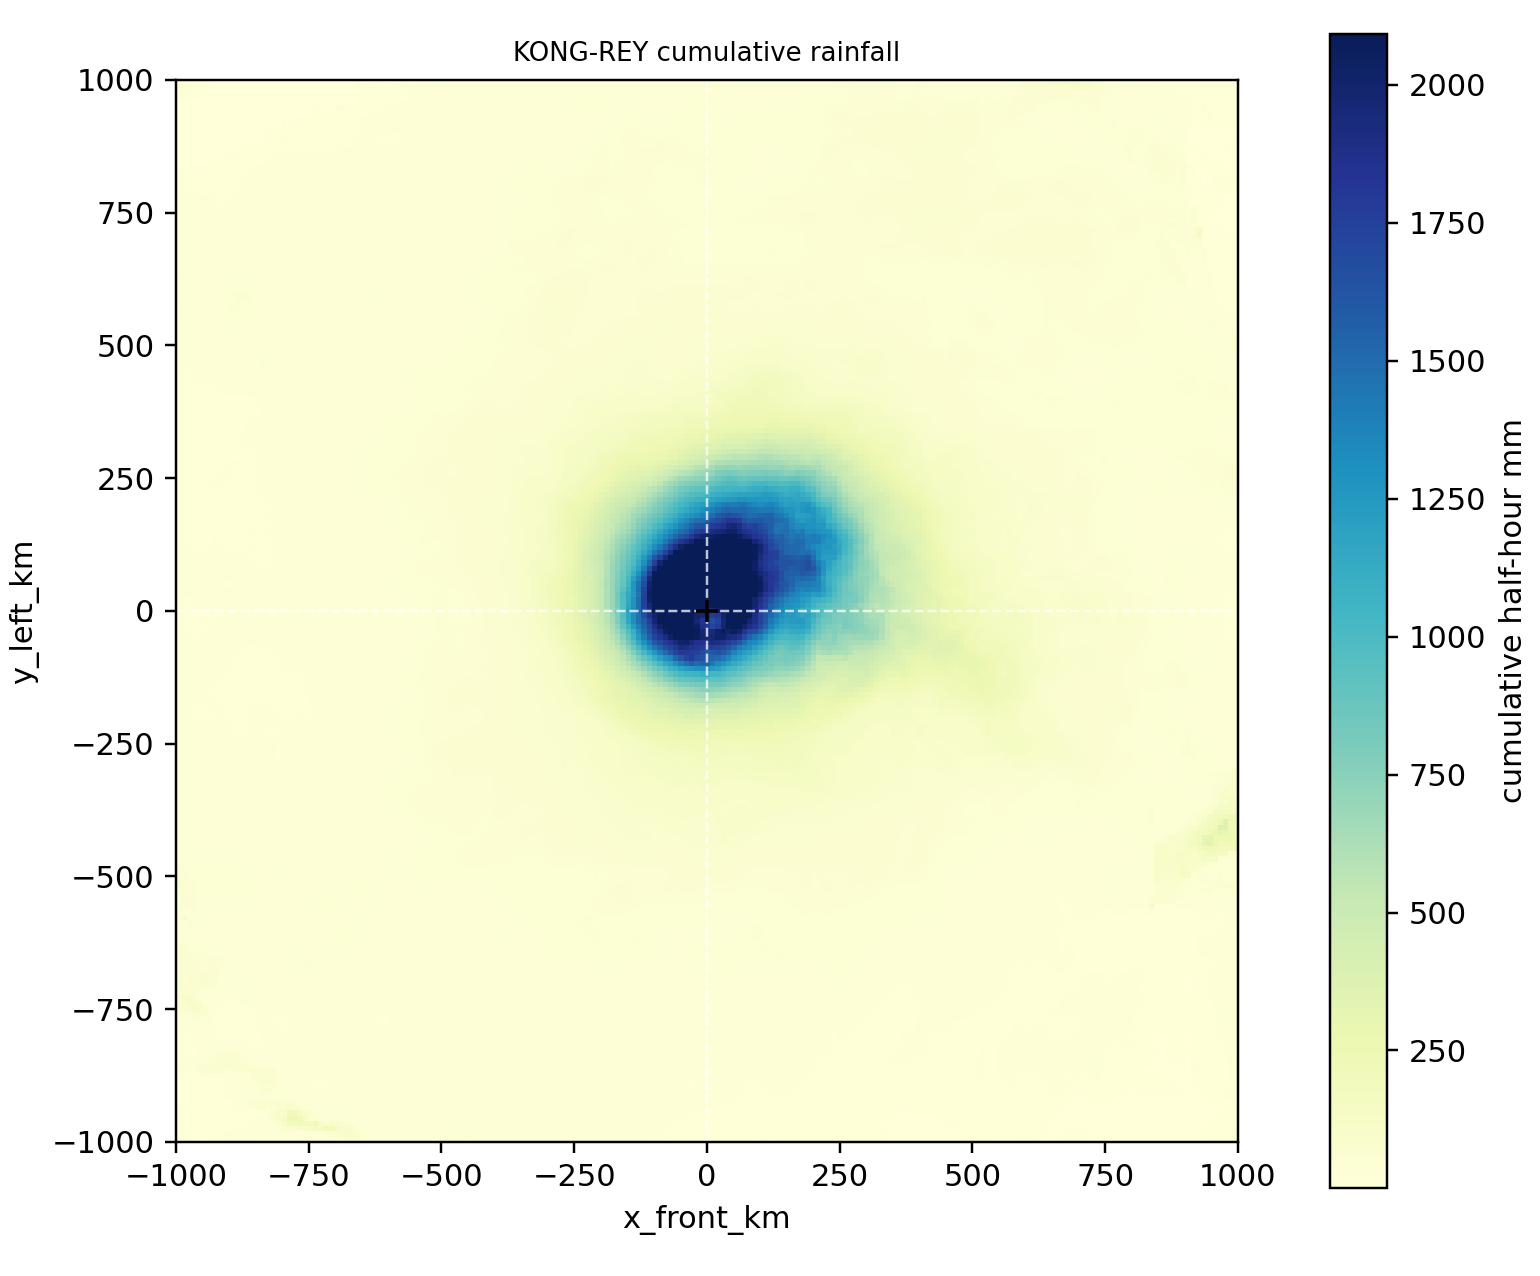
\includegraphics[width=\textwidth]{outputs/figures/problem2_env/KONG_REY_final_cumulative_rain_storm_relative.png}
\caption{KONG-REY storm-relative 累计降水结构}
\end{subfigure}
\begin{subfigure}{0.48\textwidth}
\centering
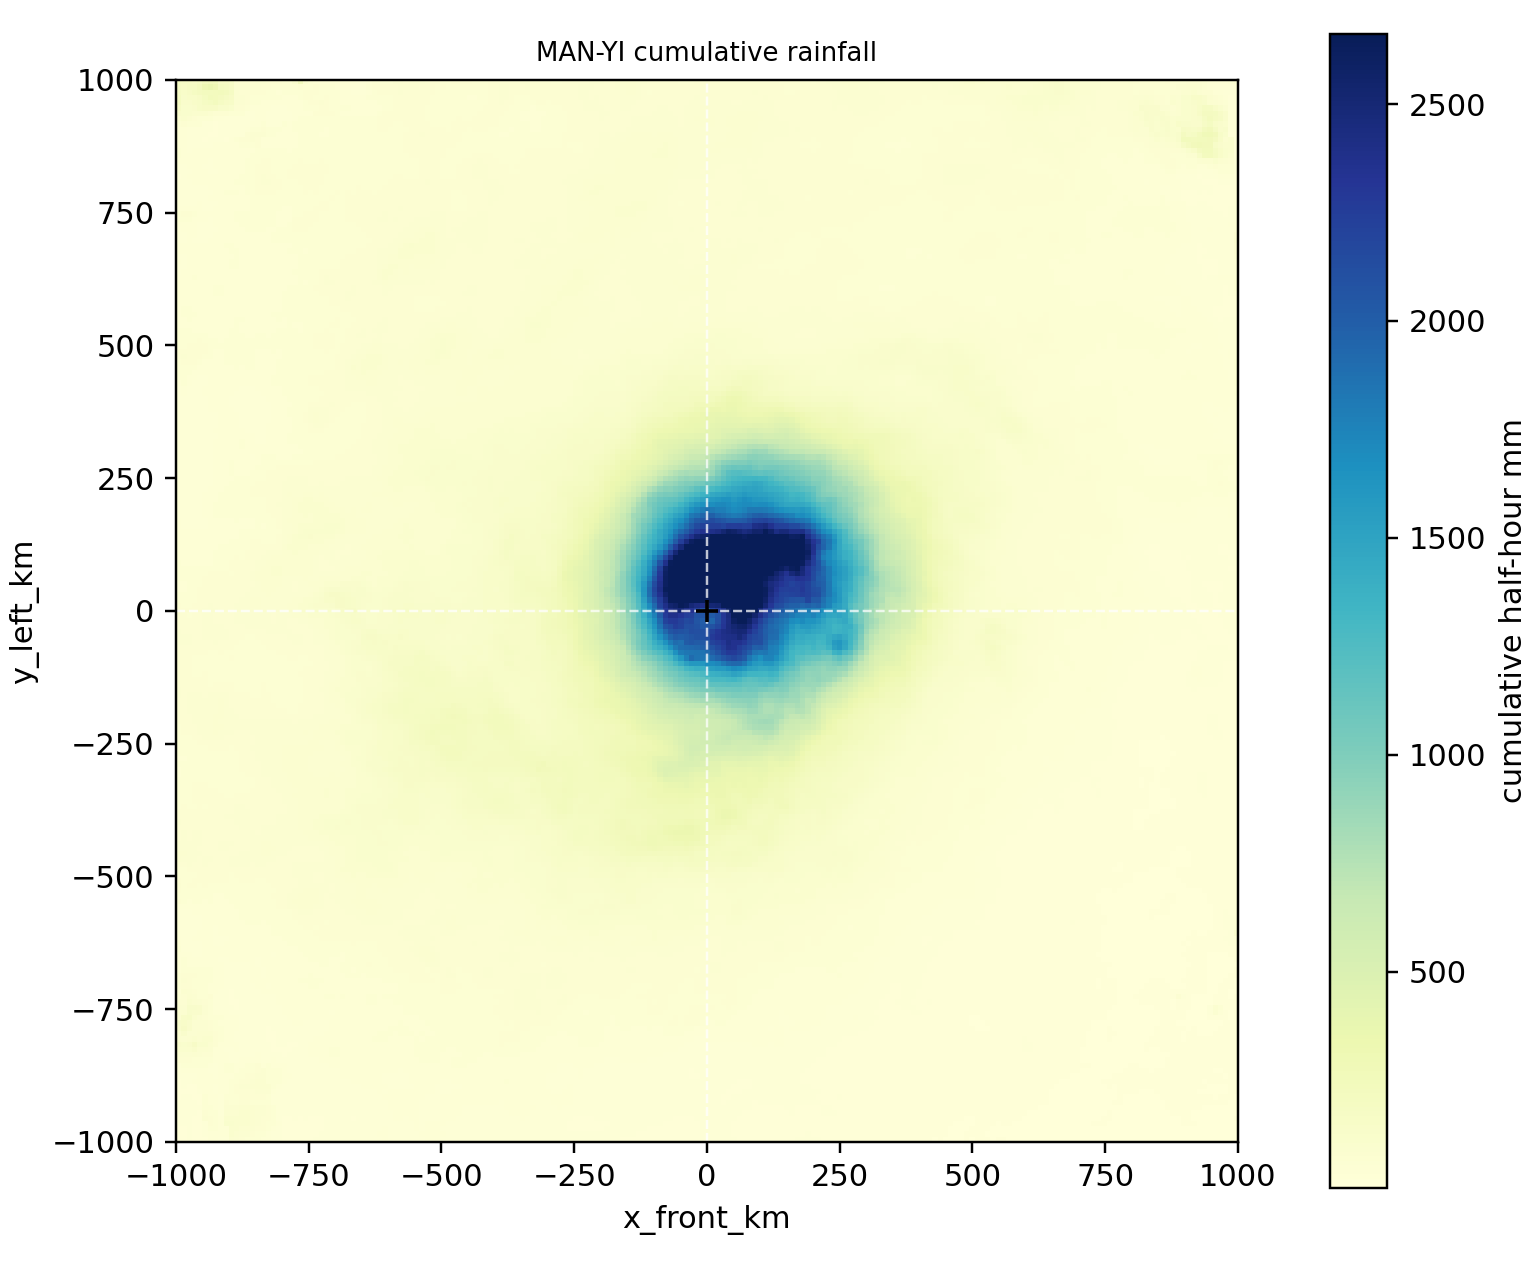
\includegraphics[width=\textwidth]{outputs/figures/problem2_env/MAN_YI_final_cumulative_rain_storm_relative.png}
\caption{MAN-YI storm-relative 累计降水结构}
\end{subfigure}
\caption{两场台风 storm-relative 累计降水结构解释图}
\label{fig:p2_cumulative_rain}
\end{figure}

\begin{figure}[H]
\centering
\begin{subfigure}{0.48\textwidth}
\centering
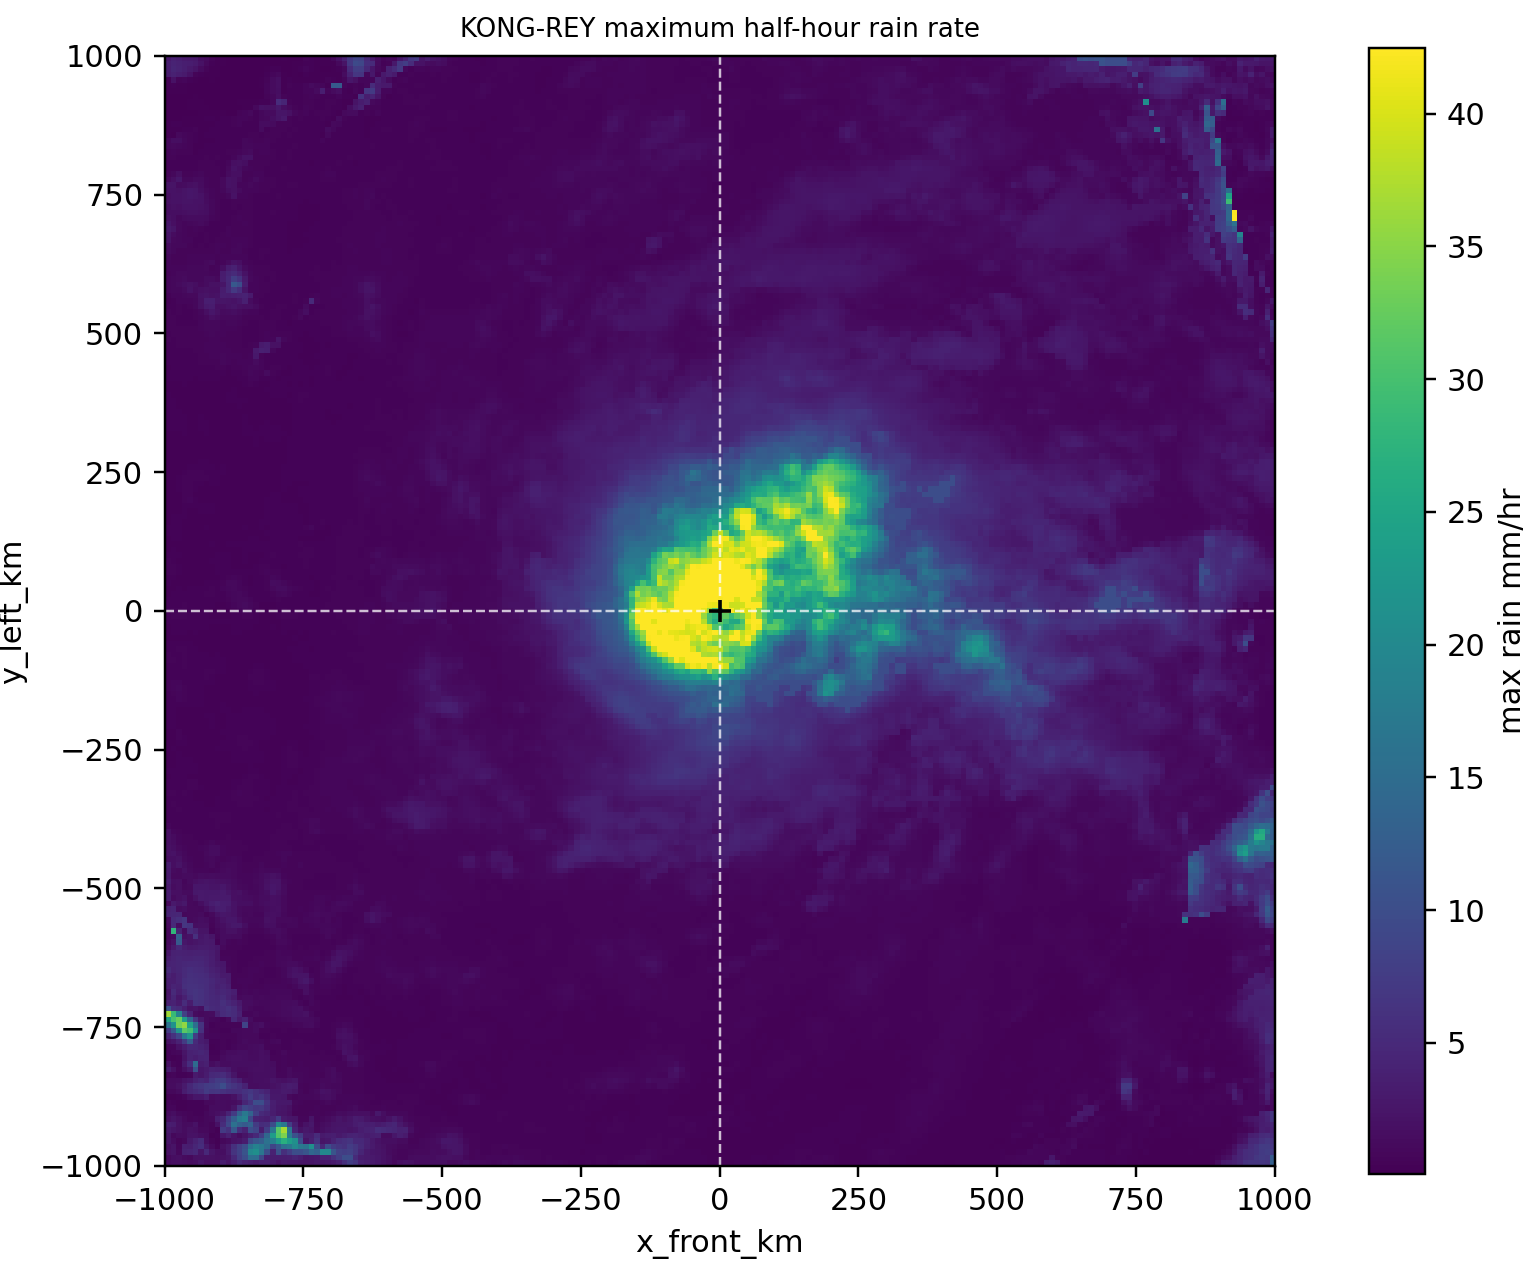
\includegraphics[width=\textwidth]{outputs/figures/problem2_env/KONG_REY_final_max_rain_storm_relative.png}
\caption{KONG-REY storm-relative 最大半小时降水结构}
\end{subfigure}
\begin{subfigure}{0.48\textwidth}
\centering
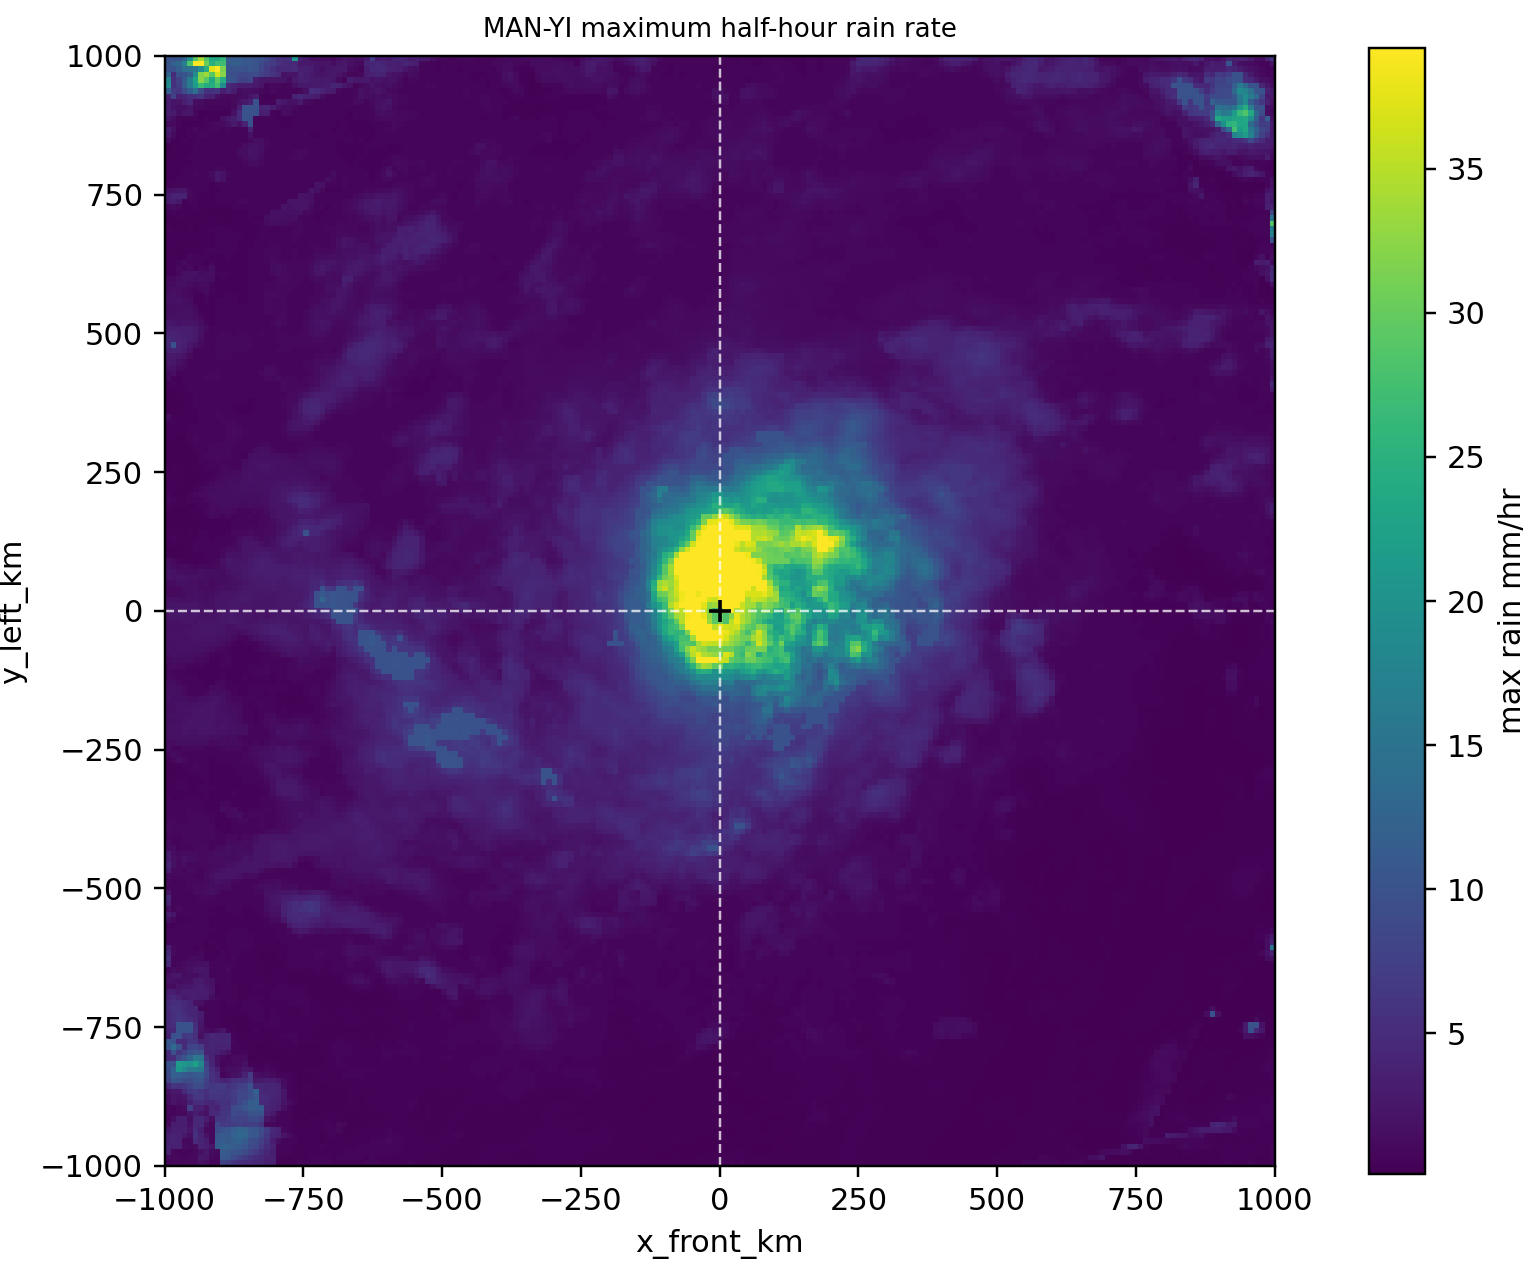
\includegraphics[width=\textwidth]{outputs/figures/problem2_env/MAN_YI_final_max_rain_storm_relative.png}
\caption{MAN-YI storm-relative 最大半小时降水结构}
\end{subfigure}
\caption{两场台风 storm-relative 最大半小时降水结构解释图}
\label{fig:p2_max_rain}
\end{figure}

\begin{figure}[H]
\centering
\begin{subfigure}{0.48\textwidth}
\centering
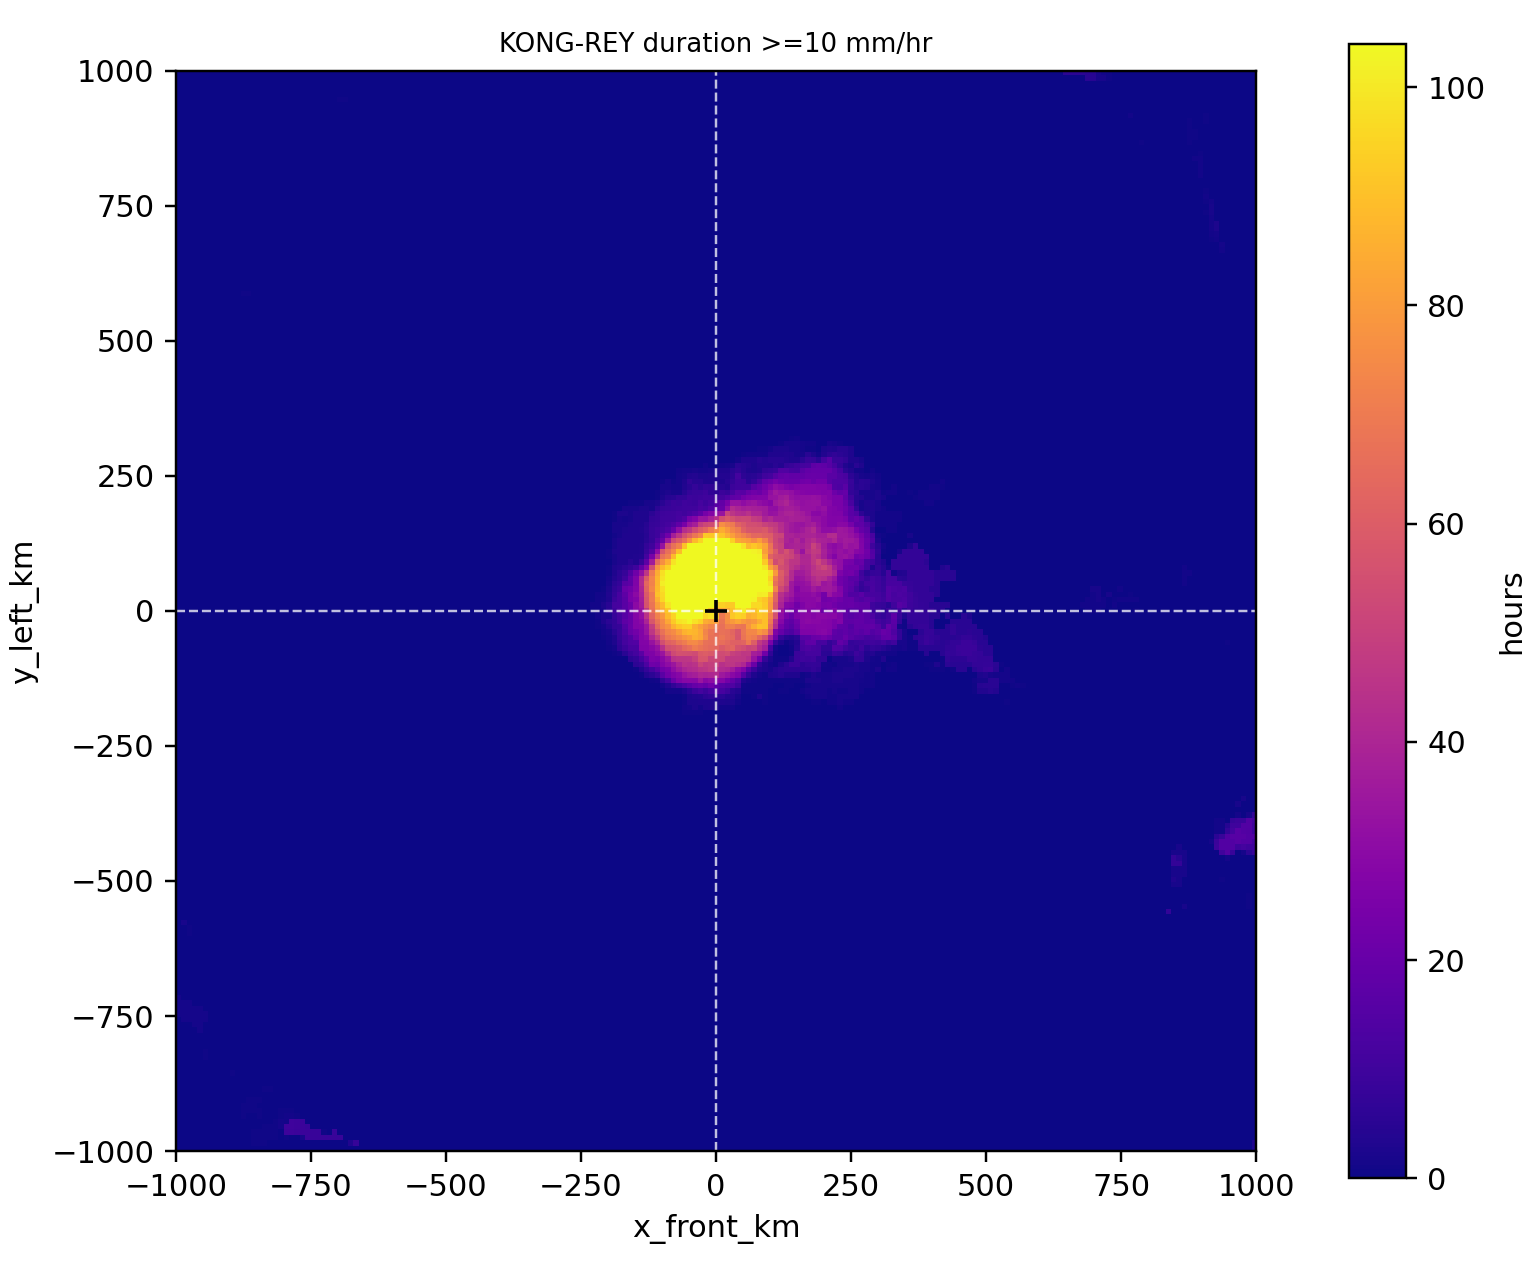
\includegraphics[width=\textwidth]{outputs/figures/problem2_env/KONG_REY_final_duration10_storm_relative.png}
\caption{KONG-REY storm-relative 强降水持续结构}
\end{subfigure}
\begin{subfigure}{0.48\textwidth}
\centering
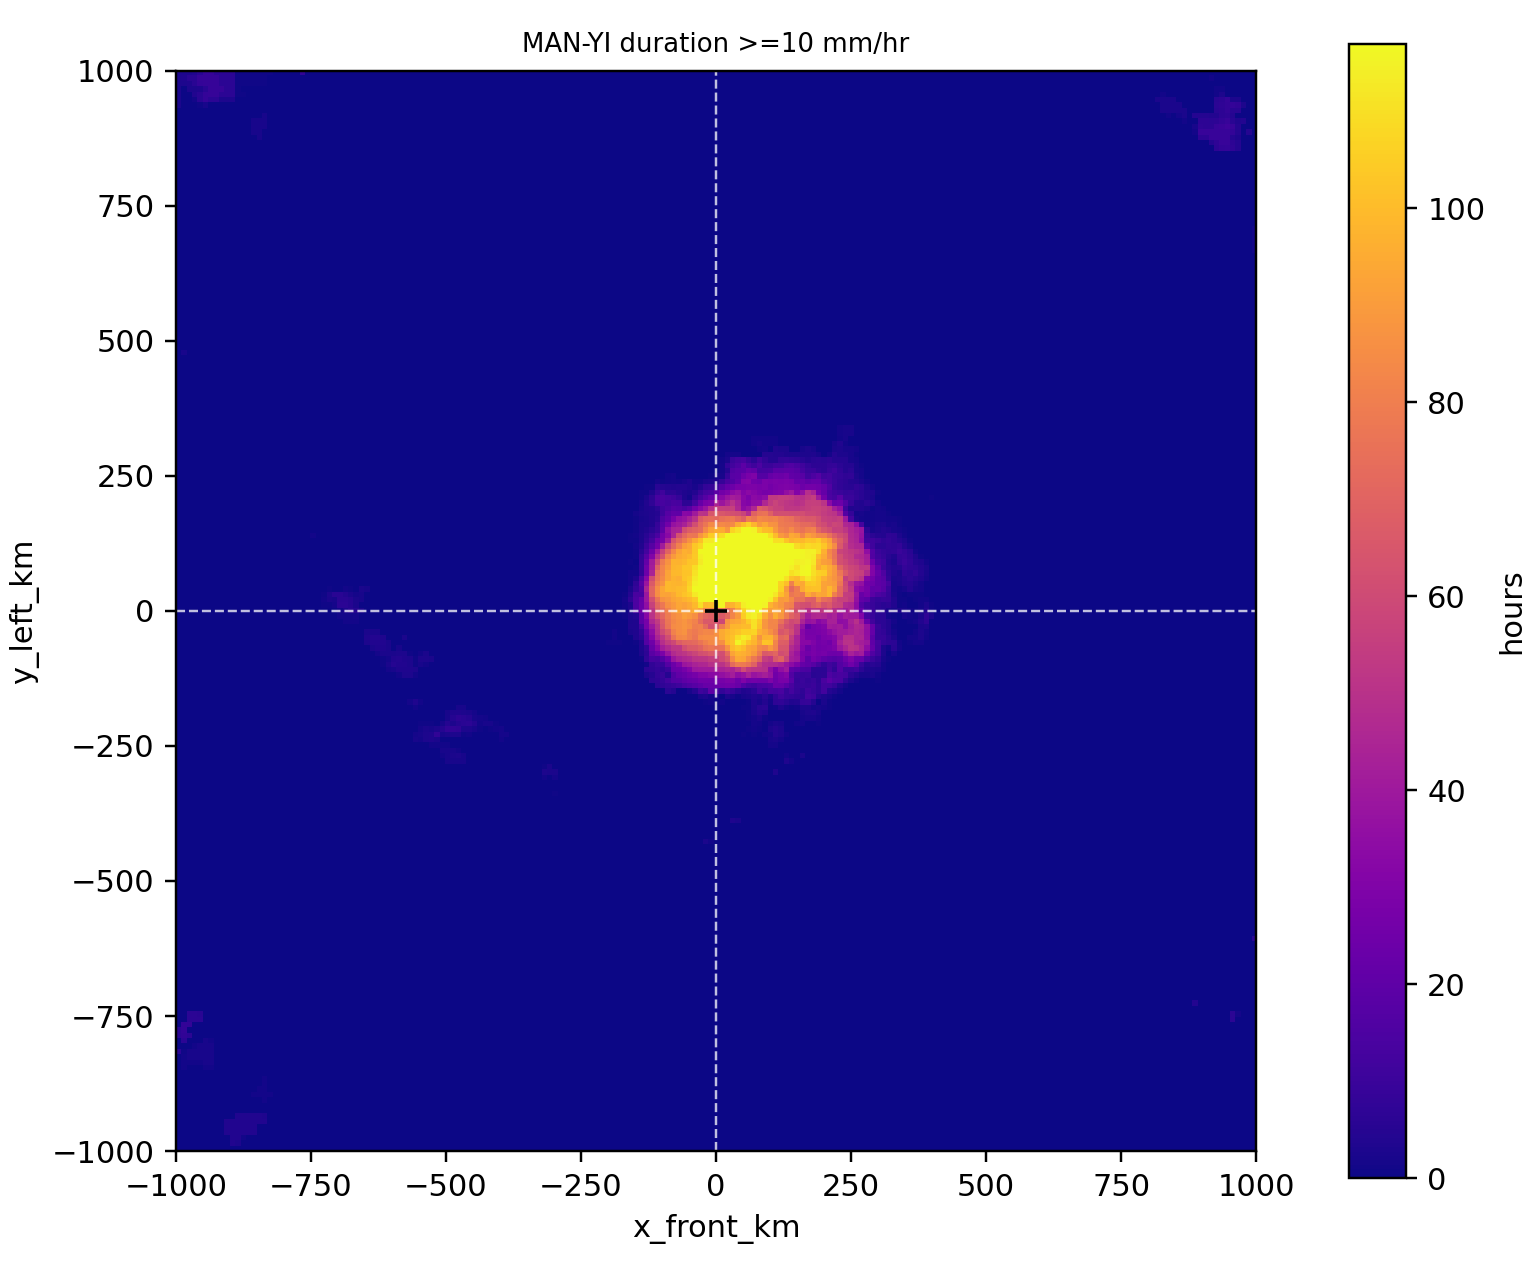
\includegraphics[width=\textwidth]{outputs/figures/problem2_env/MAN_YI_final_duration10_storm_relative.png}
\caption{MAN-YI storm-relative 强降水持续结构}
\end{subfigure}
\caption{$10\ \mathrm{mm/hr}$ 阈值下两场台风 storm-relative 强降水持续结构解释图}
\label{fig:p2_duration10}
\end{figure}

上述 storm-relative 图能够揭示台风降水结构相对于台风中心和移动方向的组织方式，但其坐标随台风中心移动而移动，并不对应固定地理位置上的降水累积。为进一步回答题目中“可能降水时空分布”的真实空间落区问题，下面将校准后的半小时降水场反投影到固定经纬度网格，计算地理累计降水和强降水持续时间。

\subsubsection{地理坐标下降水场反投影与真实落区分析}

前文给出的累计降水、最大半小时降水和强降水持续时间均是在台风相对运动坐标系下计算得到的，其主要作用是刻画降水相对于台风中心和移动方向的结构特征，例如主雨带所在象限、降水质心偏移、非对称性和雨带持续性等。该类结果有助于解释台风降水生成机理，但不能直接表示固定地理位置上的累计降水或强降水持续时间。

题目要求生成 KONG-REY 与 MAN-YI 的可能降水时空分布，因此仅给出 storm-relative 坐标下的结果是不充分的。为进一步得到真实经纬度意义下的降水落区，本文将极端分位数校准后的台风相对坐标降水场反投影到固定经纬度网格，计算地理累计降水、地理最大半小时降水和地理强降水持续时间。

设目标时刻 $t$ 的极端校准降水场为
\begin{equation}
R_t^{\mathrm{cal}}(x_f,y_l),
\end{equation}
其中 $x_f$ 表示沿台风移动方向前方的相对距离，$y_l$ 表示移动方向左侧的相对距离。记该时刻台风中心经纬度为 $(\lambda_{c,t},\phi_{c,t})$，移动方向角为 $\alpha_t$。根据台风相对运动坐标定义，可将相对坐标反变换到东西向和南北向距离：
\begin{equation}
x=x_f\sin\alpha_t-y_l\cos\alpha_t,
\qquad
y=x_f\cos\alpha_t+y_l\sin\alpha_t,
\end{equation}
其中 $x$ 表示东西向距离，$y$ 表示南北向距离，单位均为 km。

进一步将 $(x,y)$ 转换为经纬度坐标：
\begin{equation}
\lambda=\lambda_{c,t}
+\frac{x}{111.32\cos\phi_{c,t}},
\qquad
\phi=\phi_{c,t}
+\frac{y}{111.32}.
\end{equation}

实际计算时，为避免散点投影造成固定经纬度网格上的空洞，本文采用等价的反向采样方法。对固定地理网格上每个点 $(\lambda,\phi)$，先计算其相对于台风中心的东西向和南北向距离：
\begin{equation}
x=111.32\cos\phi_{c,t}(\lambda-\lambda_{c,t}),
\qquad
y=111.32(\phi-\phi_{c,t}),
\end{equation}
再转换为台风相对运动坐标：
\begin{equation}
x_f=x\sin\alpha_t+y\cos\alpha_t,
\qquad
y_l=-x\cos\alpha_t+y\sin\alpha_t.
\end{equation}
随后在 $R_t^{\mathrm{cal}}(x_f,y_l)$ 上进行双线性插值，得到固定经纬度网格上的半小时降水场
\begin{equation}
R_t^{\mathrm{geo}}(\lambda,\phi).
\end{equation}

在此基础上，定义真实地理坐标下的累计降水：
\begin{equation}
P_{\mathrm{geo}}(\lambda,\phi)
=
\sum_t 0.5 R_t^{\mathrm{geo}}(\lambda,\phi),
\end{equation}
其中 $0.5$ 为半小时累计因子，$P_{\mathrm{geo}}$ 的单位为 mm。

定义真实地理坐标下的最大半小时降水强度：
\begin{equation}
R_{\max,\mathrm{geo}}(\lambda,\phi)
=
\max_t R_t^{\mathrm{geo}}(\lambda,\phi).
\end{equation}

定义 $10\ \mathrm{mm/hr}$ 阈值下的地理强降水持续时间：
\begin{equation}
D_{10,\mathrm{geo}}(\lambda,\phi)
=
0.5\sum_t
\mathbf{1}
\left\{
R_t^{\mathrm{geo}}(\lambda,\phi)\ge 10
\right\},
\end{equation}
其中 $\mathbf{1}\{\cdot\}$ 为示性函数，$D_{10,\mathrm{geo}}$ 的单位为 h。该指标表示某一固定地理位置在整个台风过程中累计经历 $10\ \mathrm{mm/hr}$ 及以上强降水的总时长。

地理面积统计采用随纬度修正的经纬度网格面积。对于中心纬度为 $\phi$、分辨率为 $\Delta\lambda\times\Delta\phi$ 的网格单元，其面积近似为
\begin{equation}
A_{\mathrm{cell}}(\phi)
\approx
111.32^2\,\Delta\lambda\,\Delta\phi\,\cos\phi,
\end{equation}
单位为 km$^2$。因此，$P_{\mathrm{geo}}\ge100\ \mathrm{mm}$ 面积和 $D_{10,\mathrm{geo}}\ge3\ \mathrm{h}$ 面积均按满足阈值网格的 $A_{\mathrm{cell}}(\phi)$ 求和得到。

需要强调的是，$P_{\mathrm{geo}}(\lambda,\phi)$、$R_{\max,\mathrm{geo}}(\lambda,\phi)$ 和 $D_{10,\mathrm{geo}}(\lambda,\phi)$ 是用于回答真实地理空间落区的最终结果；而前文 storm-relative 坐标下的结果主要用于解释降水结构相对于台风中心和移动方向的组织形式。二者互为补充，不能相互替代。

本文以 $0.1^\circ$ 为经纬度网格分辨率，分别对 KONG-REY 与 MAN-YI 构建覆盖其路径及周边影响范围的固定地理网格。KONG-REY 的反投影网格范围为 $111.0^\circ\mathrm{E}$--$155.0^\circ\mathrm{E}$、$4.0^\circ\mathrm{N}$--$43.0^\circ\mathrm{N}$；MAN-YI 的反投影网格范围为 $103.0^\circ\mathrm{E}$--$172.0^\circ\mathrm{E}$、$2.0^\circ\mathrm{N}$--$27.0^\circ\mathrm{N}$。反投影后所有地理降水场均未出现 NaN、Inf、负值或全零异常。

图 \ref{fig:p2_geo_cum_rain} 给出了两场台风的真实地理累计降水分布。KONG-REY 的地理累计降水最大值为 $722.047\ \mathrm{mm}$，位于 $124.9^\circ\mathrm{E}$、$18.6^\circ\mathrm{N}$；MAN-YI 的地理累计降水最大值为 $533.592\ \mathrm{mm}$，位于 $153.2^\circ\mathrm{E}$、$13.9^\circ\mathrm{N}$。从局地累计峰值看，KONG-REY 更高。

\begin{figure}[H]
\centering
\begin{subfigure}{0.48\textwidth}
\centering
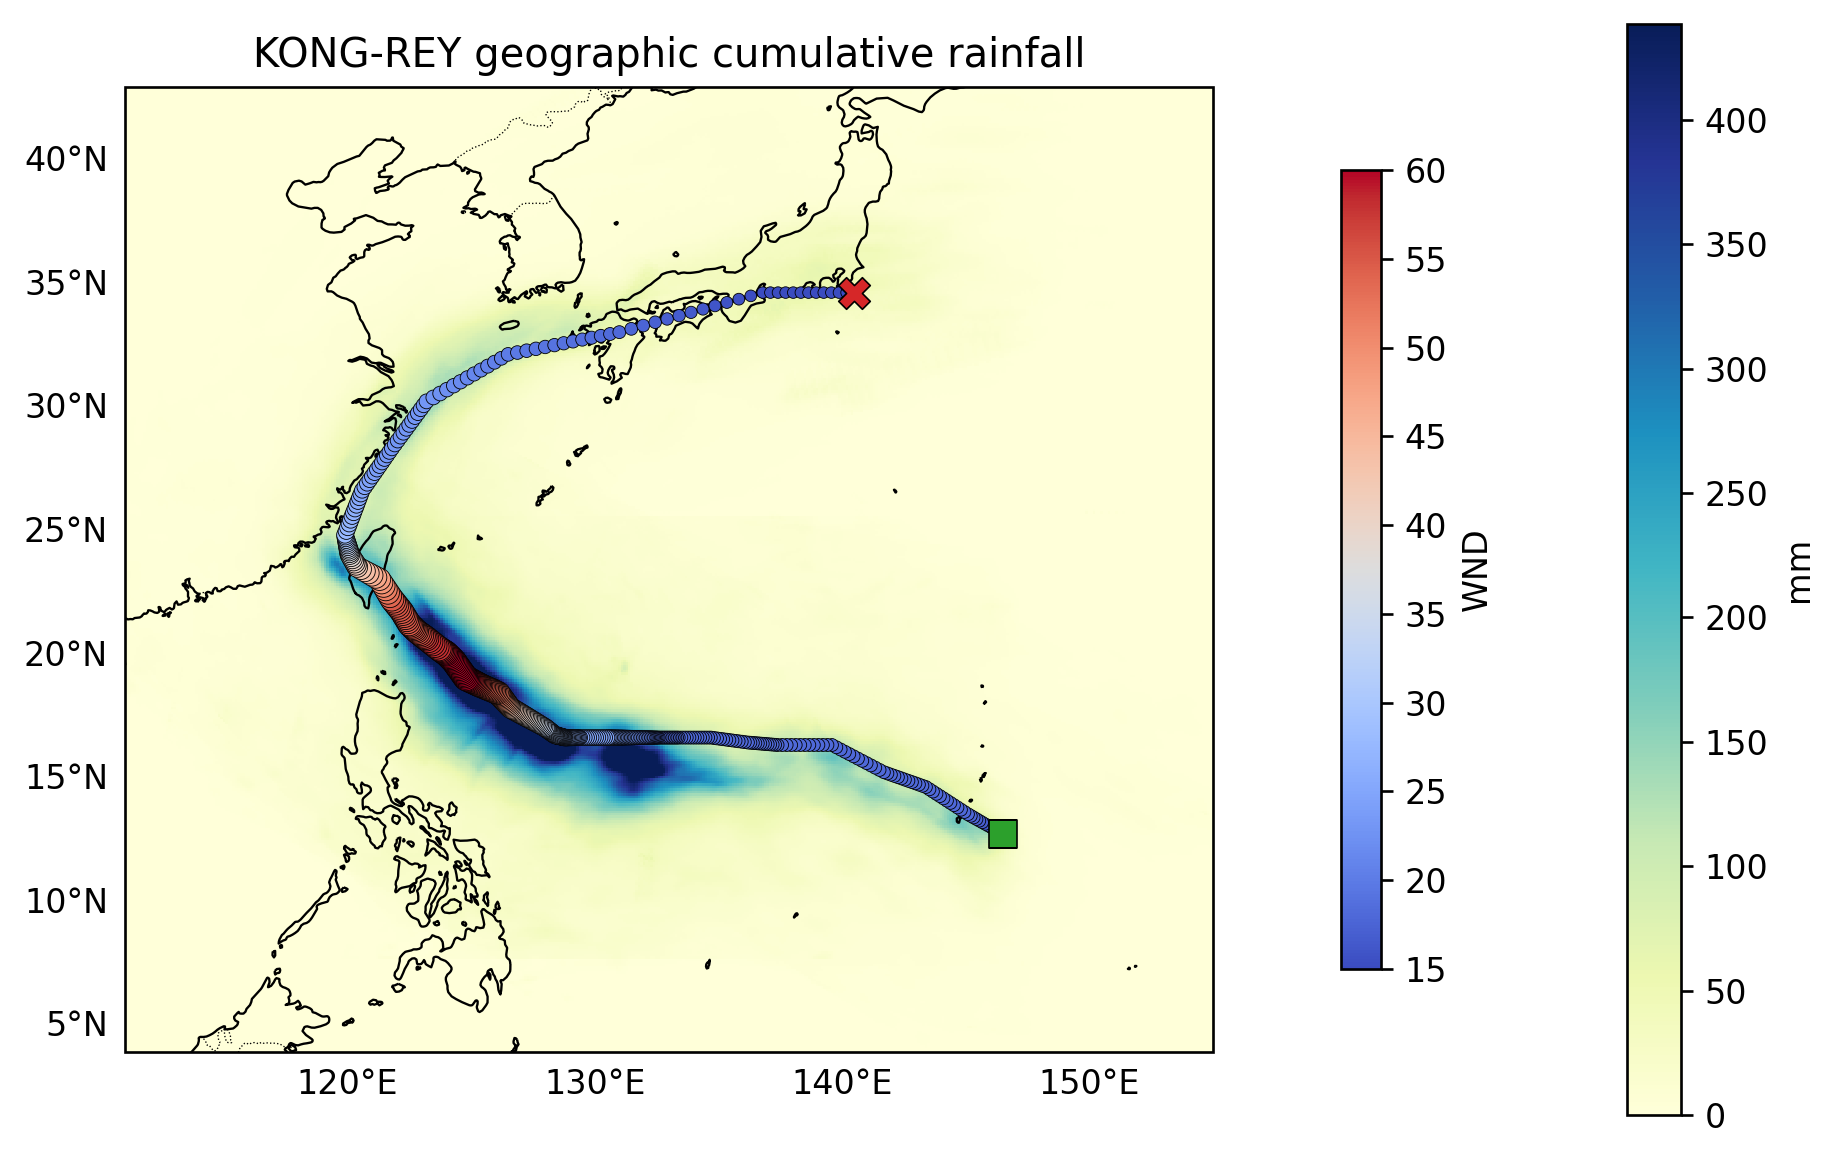
\includegraphics[width=\textwidth]{outputs/figures/problem2_env/KONG_REY_final_cumulative_rain_geographic.png}
\caption{KONG-REY 地理累计降水}
\end{subfigure}
\begin{subfigure}{0.48\textwidth}
\centering
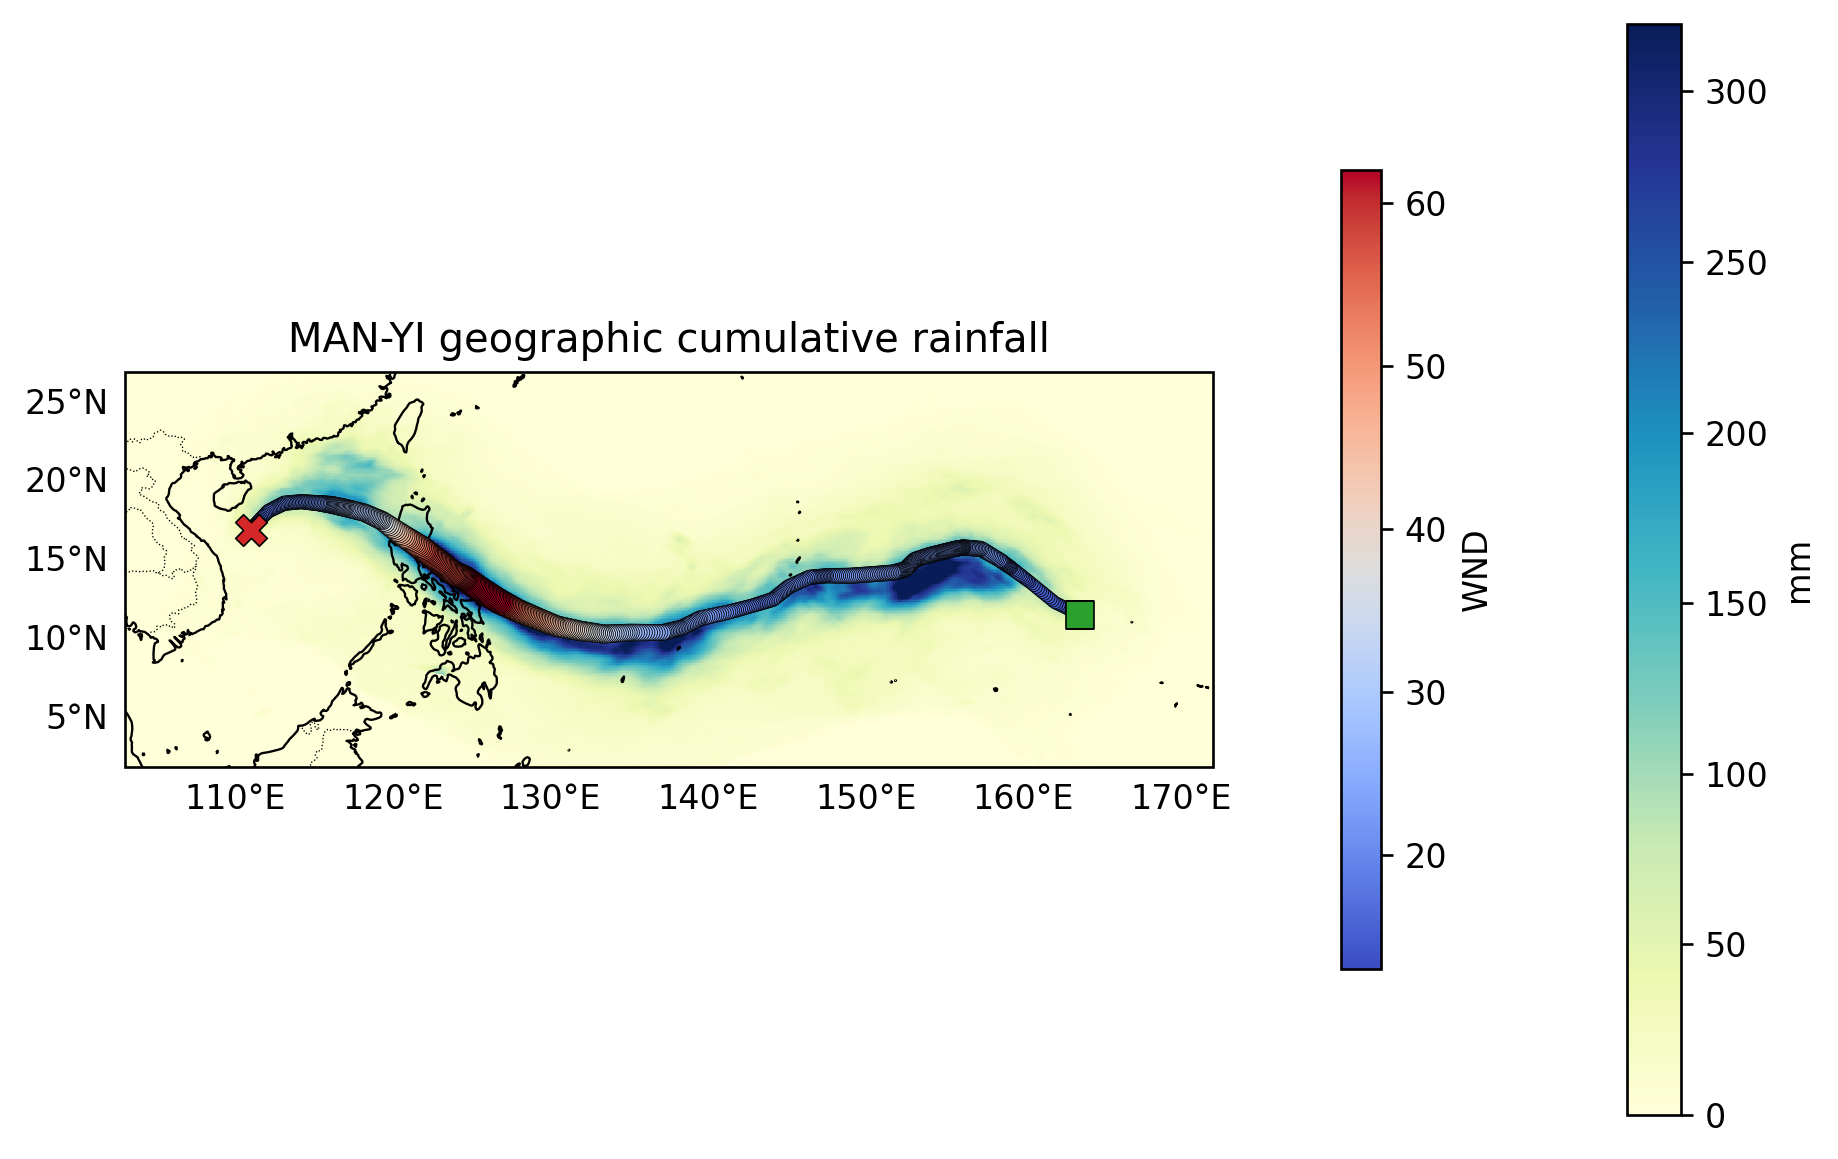
\includegraphics[width=\textwidth]{outputs/figures/problem2_env/MAN_YI_final_cumulative_rain_geographic.png}
\caption{MAN-YI 地理累计降水}
\end{subfigure}
\caption{两场台风真实地理坐标下的累计降水分布}
\label{fig:p2_geo_cum_rain}
\end{figure}

图 \ref{fig:p2_geo_max_rain} 展示了真实地理坐标下的最大半小时降水强度。KONG-REY 的最大地理半小时雨强为 $51.173\ \mathrm{mm/hr}$，发生于 2024-10-27 00:00:00，位置为 $132.2^\circ\mathrm{E}$、$15.2^\circ\mathrm{N}$；MAN-YI 的最大地理半小时雨强为 $53.529\ \mathrm{mm/hr}$，发生于 2024-11-14 10:00:00，位置为 $135.4^\circ\mathrm{E}$、$9.7^\circ\mathrm{N}$。从最大半小时雨强看，两场台风量级接近，MAN-YI 略高。

\begin{figure}[H]
\centering
\begin{subfigure}{0.48\textwidth}
\centering
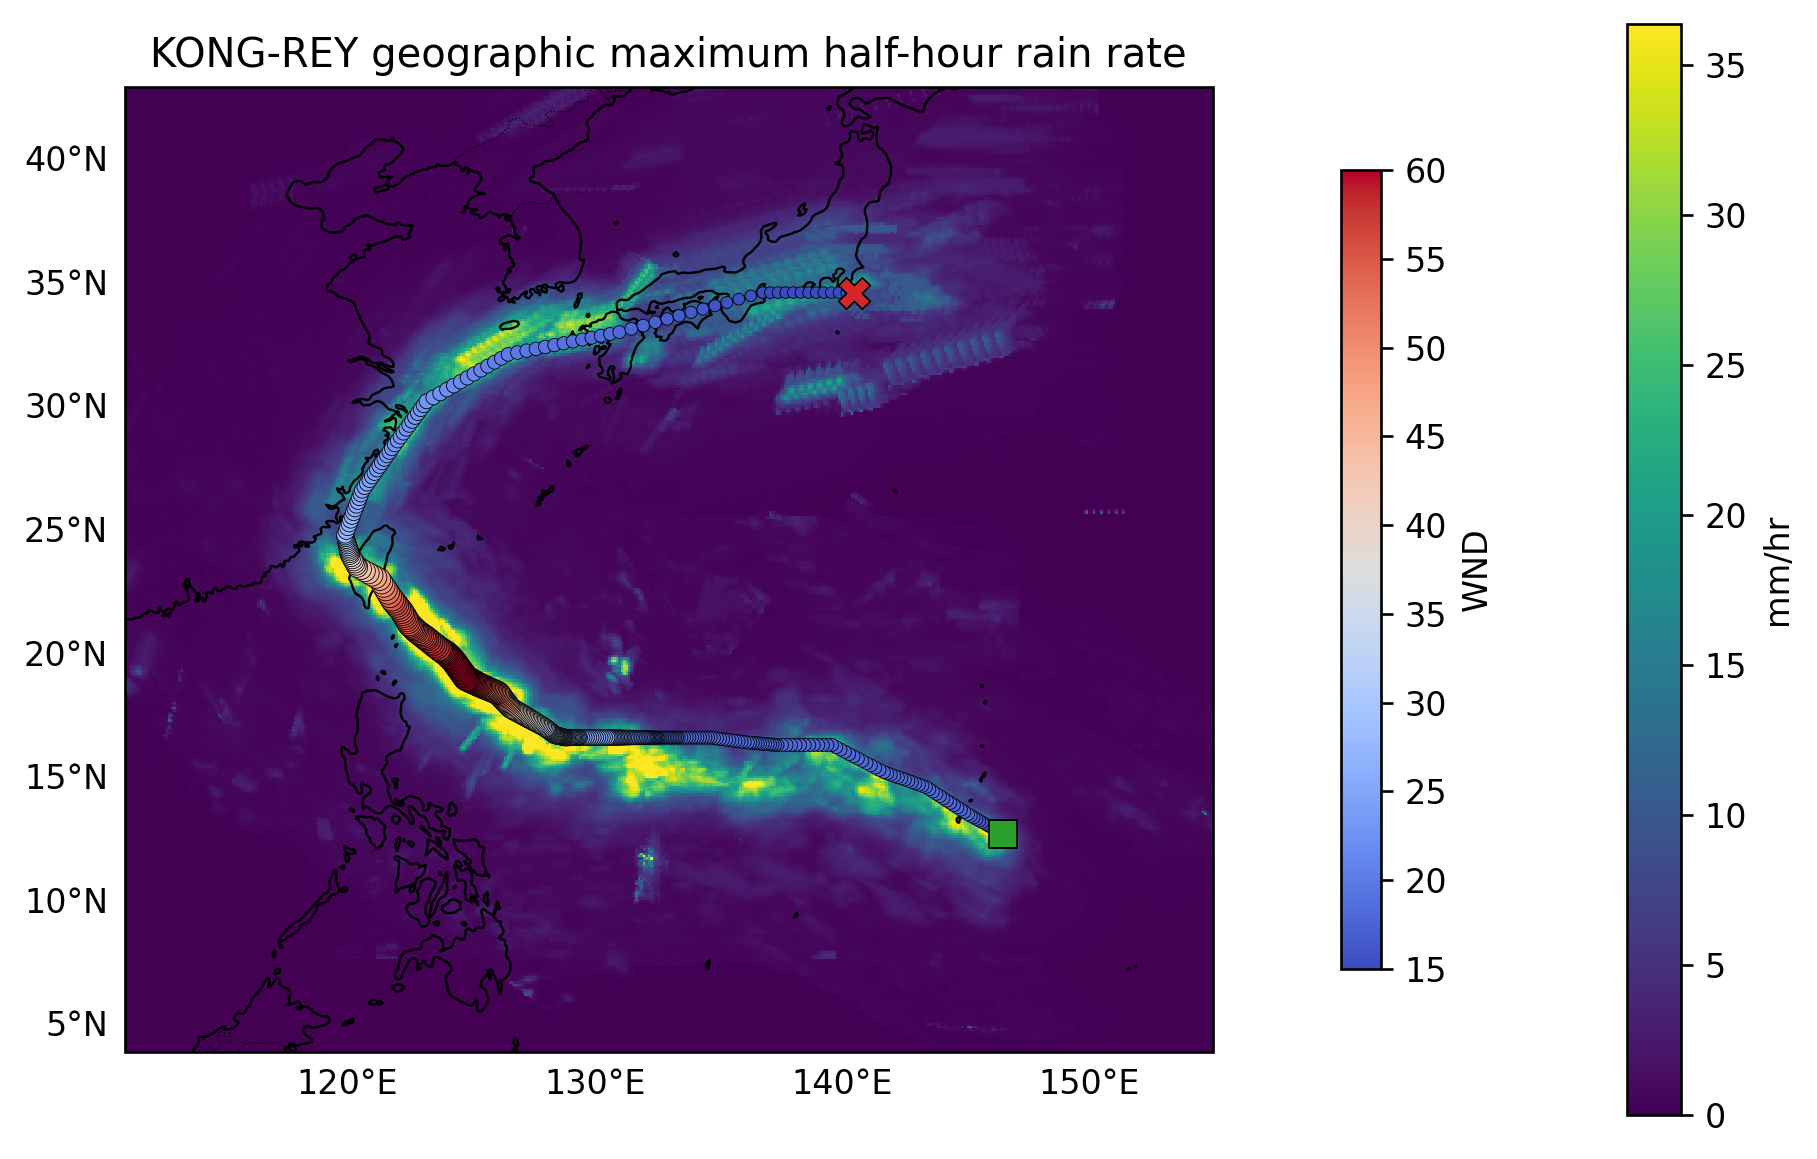
\includegraphics[width=\textwidth]{outputs/figures/problem2_env/KONG_REY_final_max_rain_geographic.png}
\caption{KONG-REY 地理最大半小时降水}
\end{subfigure}
\begin{subfigure}{0.48\textwidth}
\centering
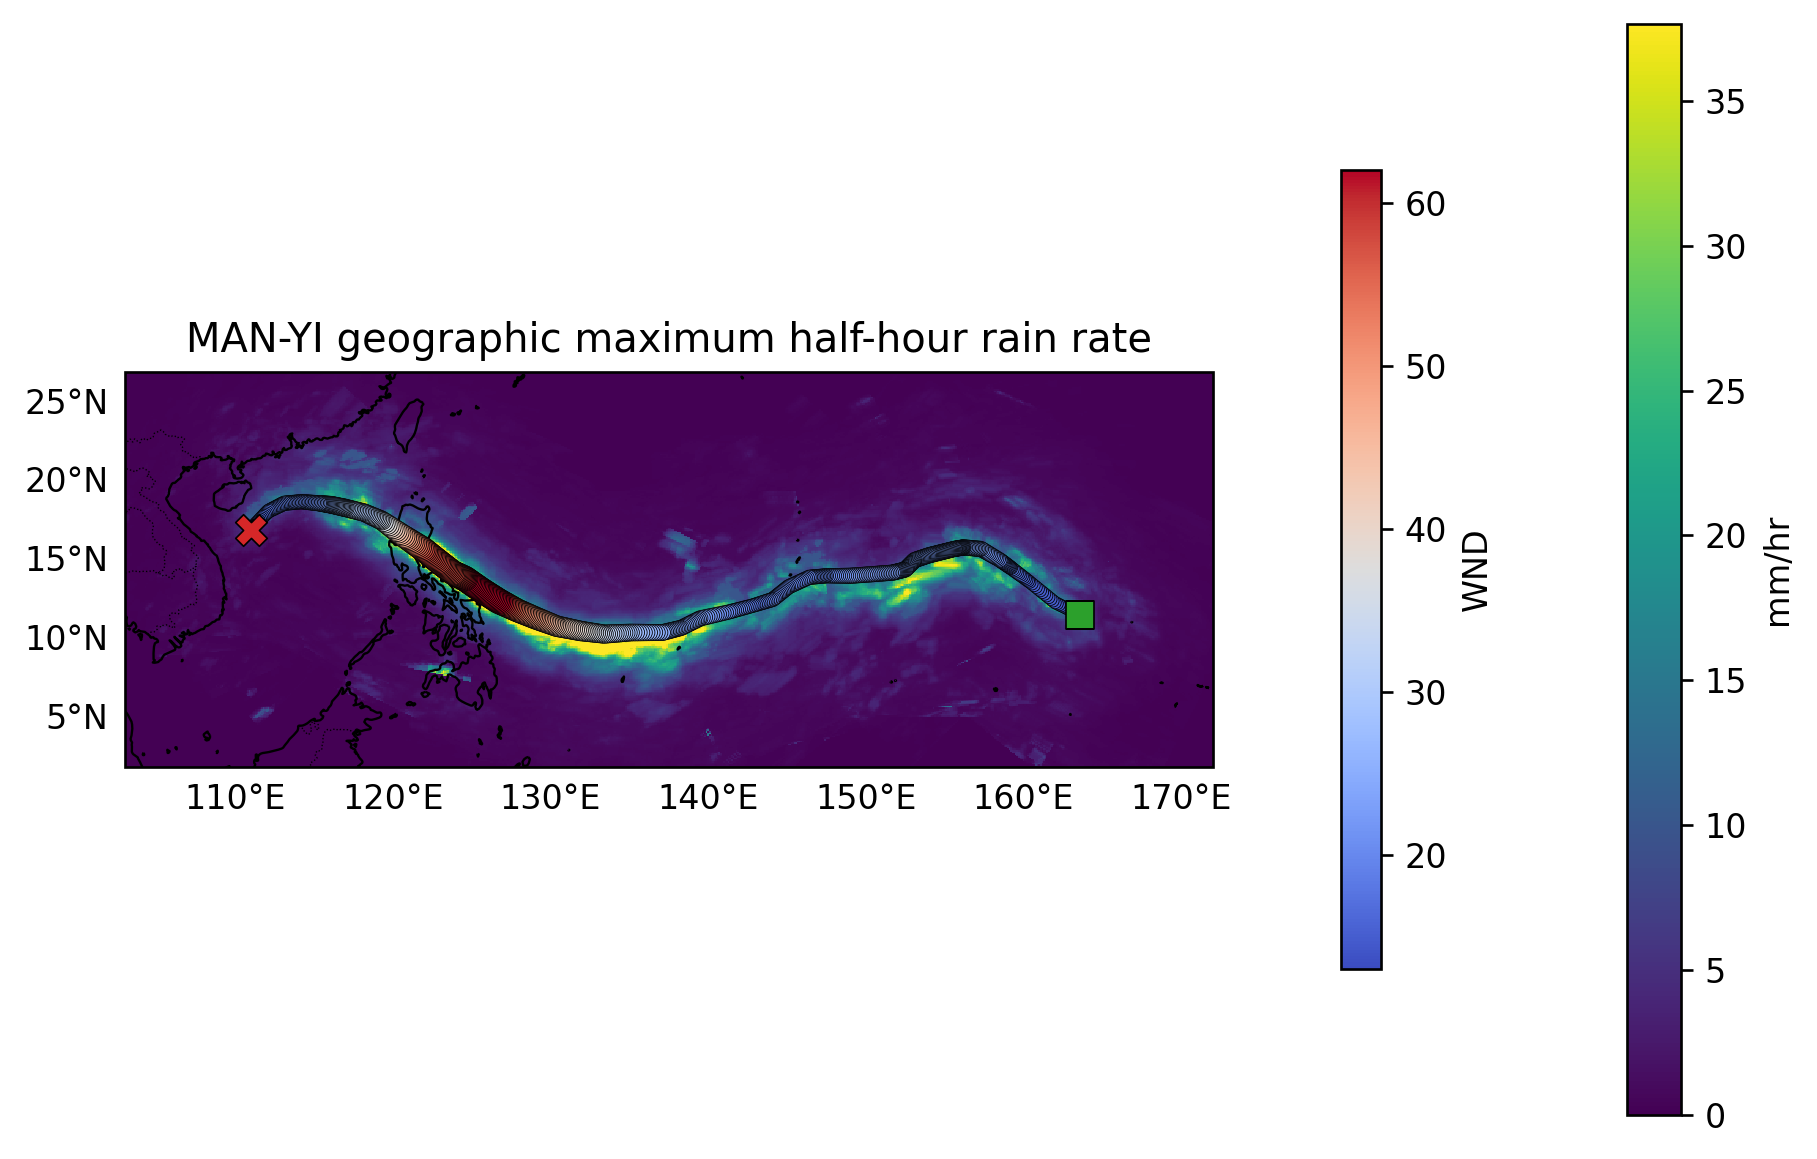
\includegraphics[width=\textwidth]{outputs/figures/problem2_env/MAN_YI_final_max_rain_geographic.png}
\caption{MAN-YI 地理最大半小时降水}
\end{subfigure}
\caption{两场台风真实地理坐标下的最大半小时降水强度分布}
\label{fig:p2_geo_max_rain}
\end{figure}

图 \ref{fig:p2_geo_duration10} 给出了 $10\ \mathrm{mm/hr}$ 阈值下的地理强降水持续时间分布。KONG-REY 的固定地理位置最大强降水持续时间为 $27.0\ \mathrm{h}$，位置为 $131.1^\circ\mathrm{E}$、$15.5^\circ\mathrm{N}$；MAN-YI 的固定地理位置最大强降水持续时间为 $23.5\ \mathrm{h}$，位置为 $153.1^\circ\mathrm{E}$、$13.8^\circ\mathrm{N}$。从单点最大持续时间看，KONG-REY 略高；但从影响范围看，MAN-YI 的 $D_{10,\mathrm{geo}}\ge3\ \mathrm{h}$ 面积达到 $1.307\times 10^6\ \mathrm{km^2}$，高于 KONG-REY 的 $8.055\times 10^5\ \mathrm{km^2}$，说明 MAN-YI 的强降水持续影响范围更广。

\begin{figure}[H]
\centering
\begin{subfigure}{0.48\textwidth}
\centering
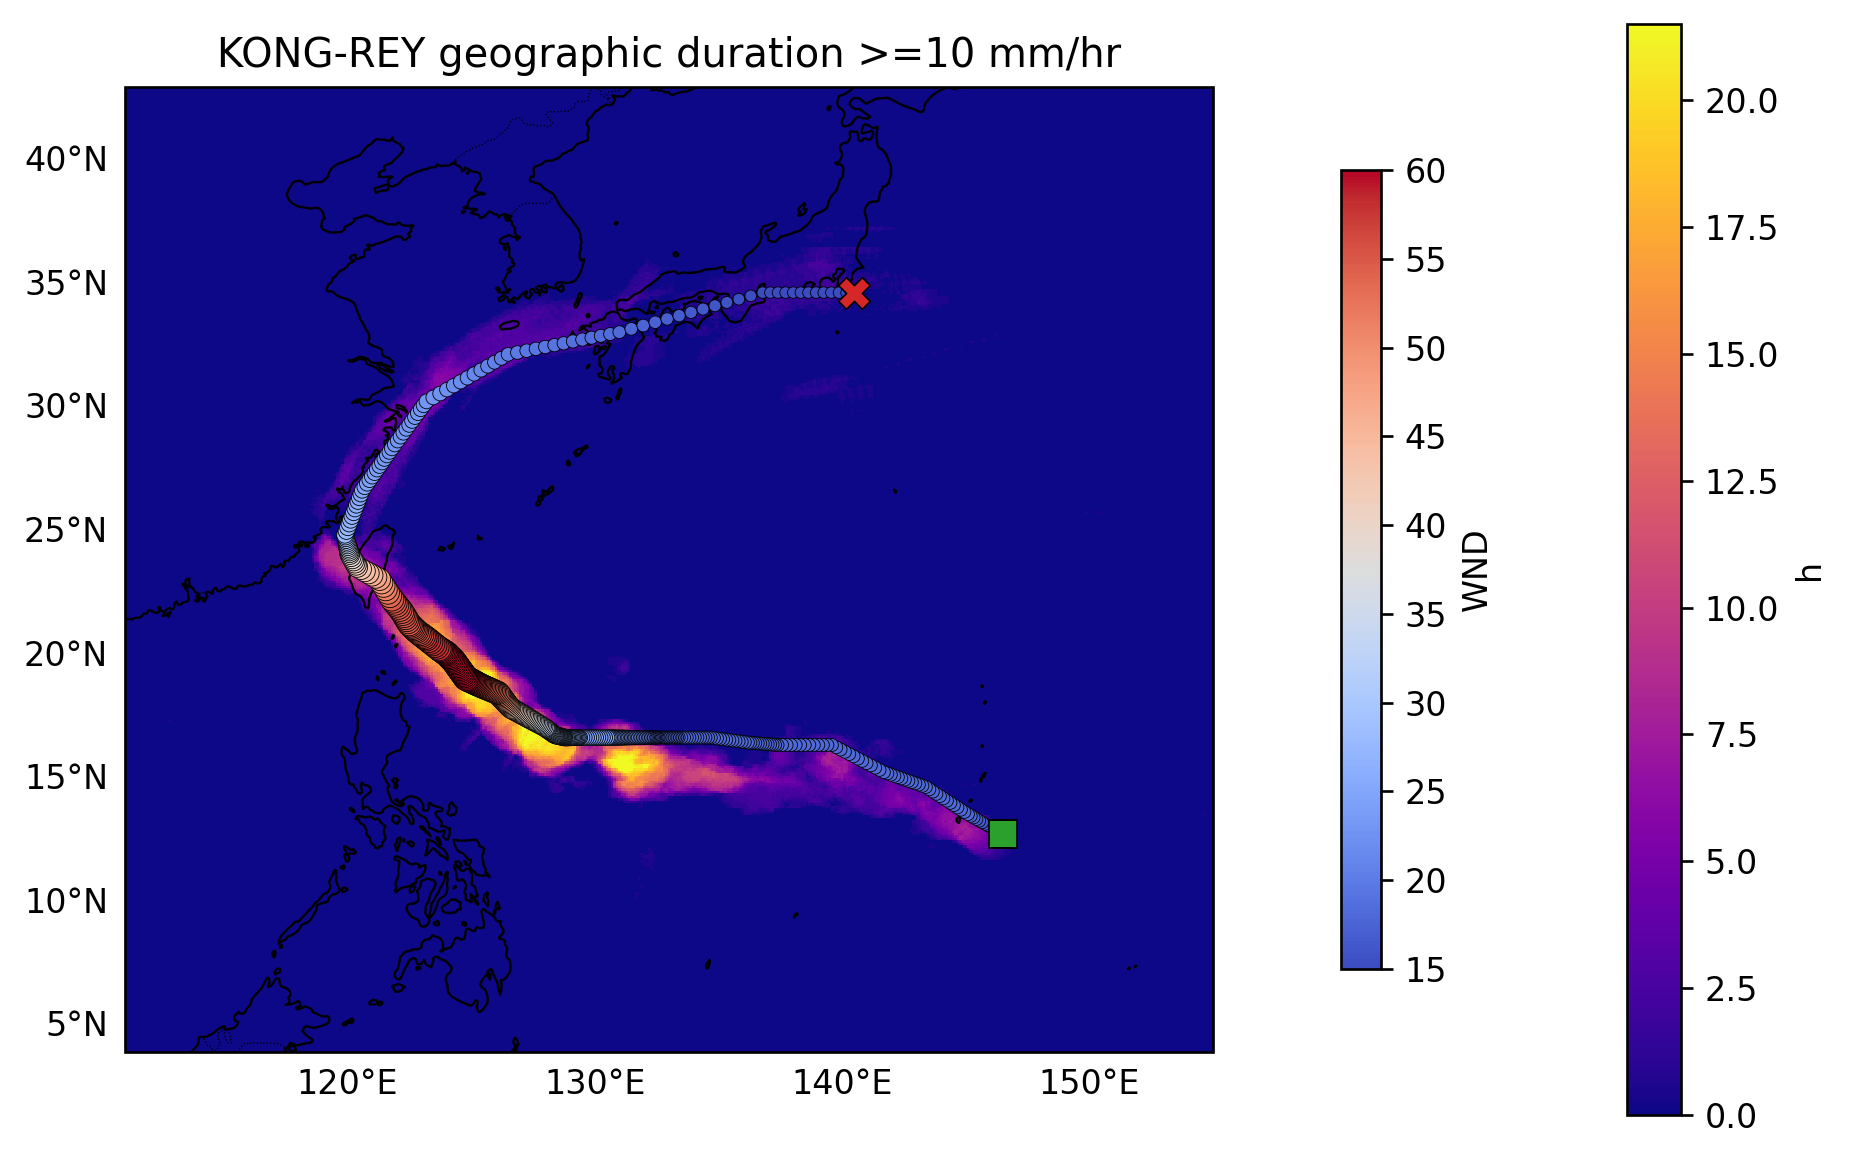
\includegraphics[width=\textwidth]{outputs/figures/problem2_env/KONG_REY_final_duration10_geographic.png}
\caption{KONG-REY 地理强降水持续时间}
\end{subfigure}
\begin{subfigure}{0.48\textwidth}
\centering
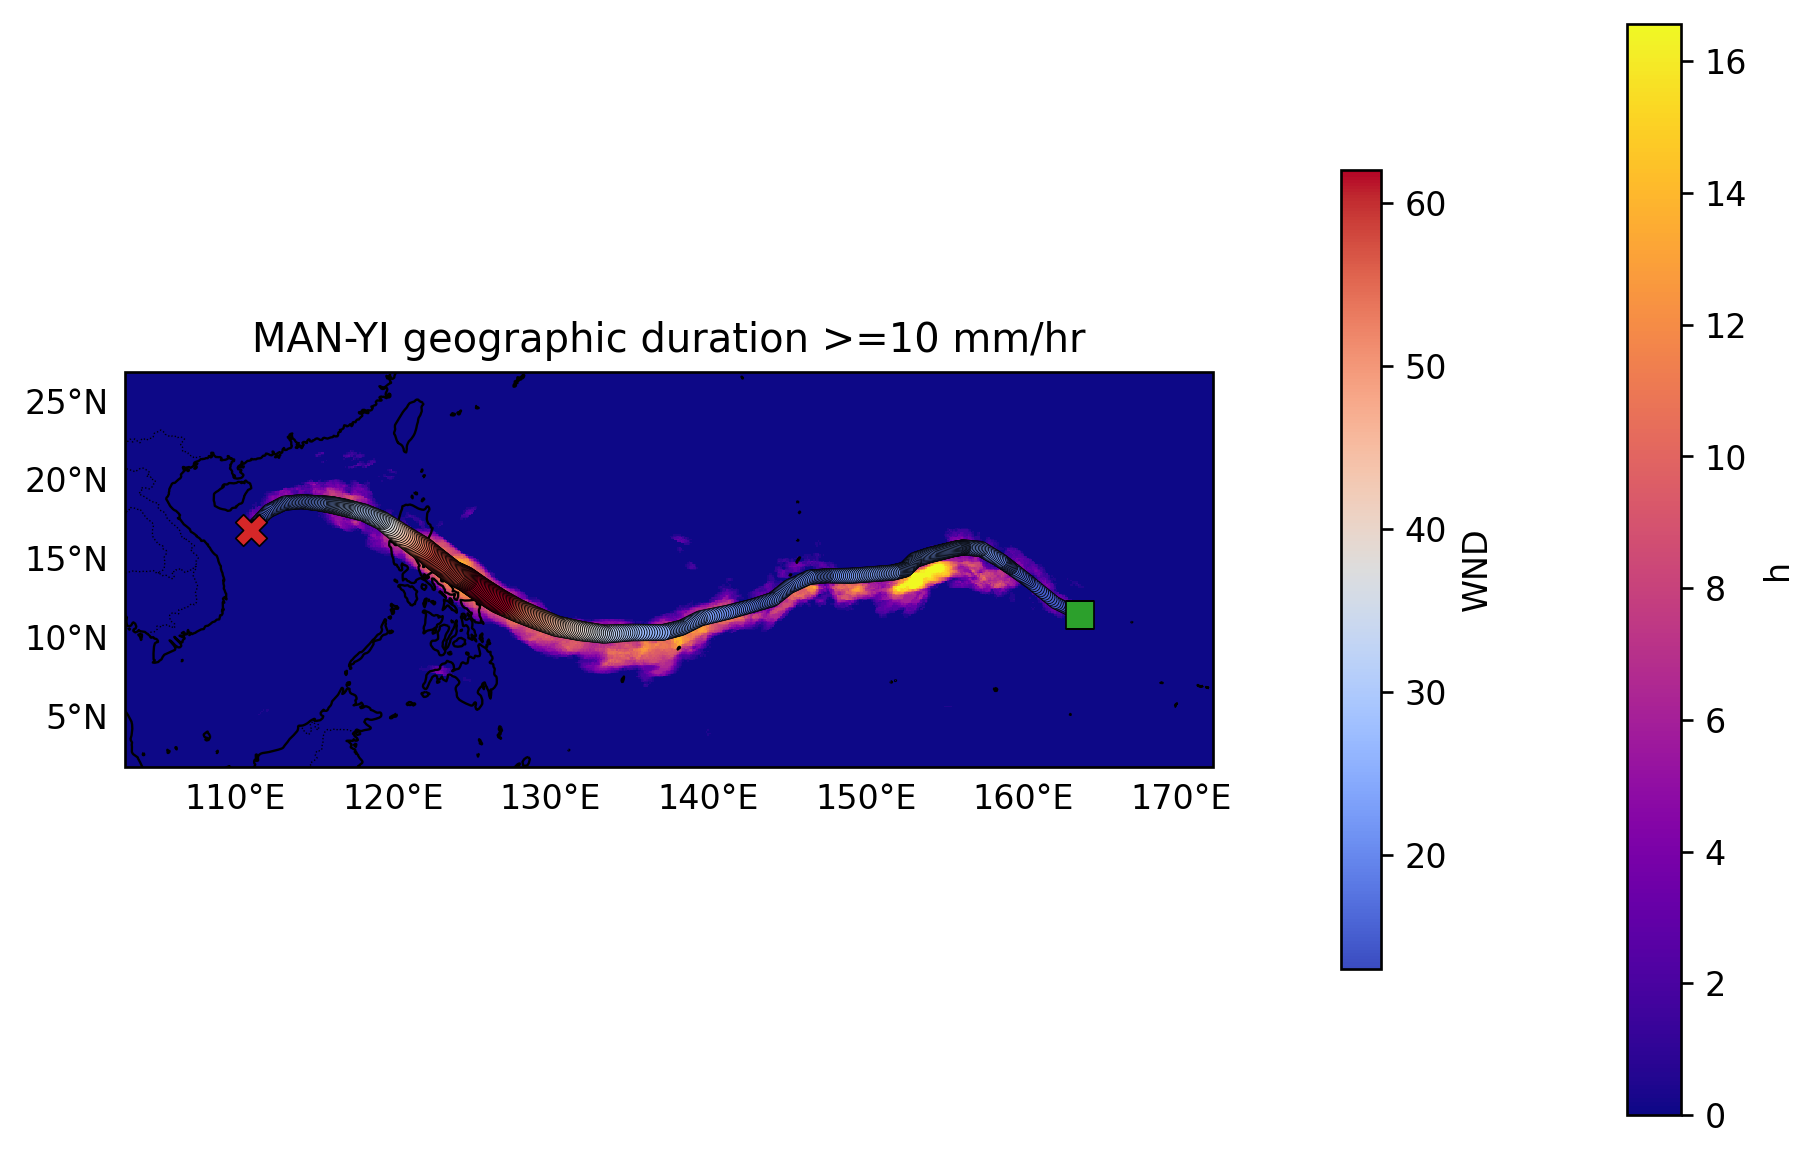
\includegraphics[width=\textwidth]{outputs/figures/problem2_env/MAN_YI_final_duration10_geographic.png}
\caption{MAN-YI 地理强降水持续时间}
\end{subfigure}
\caption{$10\ \mathrm{mm/hr}$ 阈值下两场台风真实地理强降水持续时间分布}
\label{fig:p2_geo_duration10}
\end{figure}

综合地理反投影结果可知，KONG-REY 的局地累计降水峰值更高，其最大累计降水点出现在 $124.9^\circ\mathrm{E}$、$18.6^\circ\mathrm{N}$ 附近；MAN-YI 的地理影响范围更广，其累计降水超过 $100\ \mathrm{mm}$ 的面积为 $2.071\times 10^6\ \mathrm{km^2}$，高于 KONG-REY 的 $1.229\times 10^6\ \mathrm{km^2}$。因此，从局地极端累计量看，KONG-REY 更突出；从大范围持续强降水影响看，MAN-YI 更突出。

至此，本文同时给出了两类结果：一类是台风相对坐标下的降水结构图，用于解释降水相对于台风中心和移动方向的非对称组织；另一类是真实地理坐标下的降水落区图，用于回答固定经纬度区域的可能累计降水、最大半小时雨强和强降水持续时间。二者共同构成 KONG-REY 与 MAN-YI 可能降水时空分布的最终展示。

综上，问题二所建模型在不使用目标台风真实降水记录的前提下，依据历史相似台风的路径、强度、移动和海陆环境条件，生成了 KONG-REY 与 MAN-YI 的半小时降水时空分布。伪缺失验证表明，极端校准后的模型显著提高了 P95、P99 和强降水面积的恢复能力，因此本文将 calibrated 场作为两场台风的最终可能降水分布结果。

\section{问题三模型建立与求解}

\subsection{建模思路}

第三问以问题二建立的路径--强度--环境--降水条件生成模型为基础，不另建新的降水模型。考虑到未来气候变化背景下台风路径、强度和移动速度可能偏离历史统计特征，本文将这种偏离理解为情景扰动动机，而不是确定性预报；扰动幅度仍限制在历史可比样本支持范围内。虚拟台风情景通过扰动台风路径、强度、移动速度等输入变量构造，并将扰动后的输入重新送入条件降水场生成链条，从而生成对应的半小时降水时空分布。

该过程不直接平移已有雨场，也不对基准雨场进行整体倍数放大，因此情景差异来自路径、强度、运动和环境条件共同作用下的模型响应。评价指标围绕极端降水量、强降水面积、固定地理格点持续时间和影响区域变化展开。由于 GPM 降水场的雨强单位为 $\mathrm{mm\,h^{-1}}$，而每个时次对应半小时，事件累计降水必须乘以 $0.5$ 的时间因子，不能将雨强直接累加为累计降水。

\subsection{虚拟台风情景构造}

本文以 KONG-REY 为基准台风构造 S0 情景，并在历史可比样本约束下设置五类扰动情景。S0 为基准情景，保持问题二输入不变；S1 为强度增强情景，仅扰动 WND 和 PRES，并保持风速增强与气压降低的一致性；S2 为路径近岸或西移情景，主要改变经度，使路径更靠近我国沿海；S3 为登陆点或近岸段偏移情景，仅在距岸最近附近施加平滑路径扰动；S4 为移动速度减慢情景，通过拉长时间轴降低沿路径推进速度；S5 为复合高风险情景，采用半幅强度、半幅路径和轻度减速的组合扰动。各情景的具体扰动幅度和构造方式见表~\ref{tab:problem3_scenarios}。

\begin{table}[H]
  \centering
  \footnotesize
  \setlength{\tabcolsep}{3pt}
  \renewcommand{\arraystretch}{1.16}
  \caption{问题三虚拟台风情景构造}
  \label{tab:problem3_scenarios}
  \begin{tabularx}{\linewidth}{c p{2.1cm} p{3.9cm} X X}
    \toprule
    情景 & 控制因子 & 扰动幅度 & 构造方式 & 物理含义 \\
    \midrule
    S0 & 基准 & 无扰动 & 保持 KONG-REY 的问题二输入不变 & 作为所有扰动情景的内部对照 \\
    S1 & 强度增强 & $WND'=\min(WND+8.00,\ 66.50)$ m/s；$PRES'=\max(PRES-1.748\Delta WND,\ 908.33)$ hPa & 增大 WND，并依据历史 WND--PRES 拟合关系同步降低 PRES；路径和移动过程不变 & 表征强度增强但路径和移动过程不变的情景 \\
    S2 & 路径近岸/西移 & 整条路径西移 $100\ \mathrm{km}$，即 $\Delta\lambda=100/(111.32\cos\varphi)$ & 仅改变经度并重算移动、距岸、海陆覆盖和地形变量 & 表征相同强度台风更靠近我国沿海的影响 \\
    S3 & 近岸段偏移 & 距岸最近时刻峰值北移 $75\ \mathrm{km}$，时间权重为 $\exp[-0.5((t-t_0)/24\mathrm{h})^2]$ & 仅在距岸最近附近施加平滑局地路径扰动，并重算空间环境变量 & 表征登陆点或近岸影响带位置变化 \\
    S4 & 移动速度减慢 & 时间轴拉伸系数 $1/\gamma=1/0.651\approx1.54$；沿路径速度为 S0 的 $0.651$ 倍 & 按 $\mathrm{elapsed}_{old}=\gamma\mathrm{elapsed}_{new}$ 插值路径和强度，并重新生成半小时时次 & 表征台风滞留增强导致固定地点暴露时间延长 \\
    S5 & 复合高风险 & 半幅扰动：$0.5\times$S1 强度增量、$0.5\times$S2 西移，即 $50\ \mathrm{km}$；$\gamma=0.825$ & 先施加半幅 WND/PRES 扰动，再西移 50 km，最后进行轻度时间轴拉伸 & 表征多种不利因素共同作用的风险响应 \\
    \bottomrule
  \end{tabularx}
\end{table}

上述幅度由可比历史样本约束得到：S1 和 S5 的强度扰动被限制在历史 WND 的 $P_{99}=66.50\ \mathrm{m/s}$ 与 PRES 的 $P_{01}=908.33\ \mathrm{hPa}$ 以内；S4 的 $\gamma=0.651$ 来自历史中位移速与 KONG-REY 平均移速之比，并裁剪在 $[0.65,0.80]$。有效性审计显示，S4 的 WND、PRES、移动速度和距岸距离均落在可比历史样本 min--max 范围内；S0、S1 和 S3 的少量样本外值来自 KONG-REY 观测路径本身的高速尾部，S2 和 S5 仅在近岸零距离附近出现有限沿岸边界外延，整体仍处于历史 min--max 或沿岸可比范围内。

在变量使用上，OWD 字段因在 CMABSTdata 中缺失而不纳入情景扰动；\verb|rain_*|、\verb|centroid_*|、\verb|anisotropy|、\verb|asym_*|、\verb|quad_*| 以及由降水场反推的半径类指标属于目标降水派生变量，若用于目标台风生成会造成数据泄漏，因此均不作为输入变量。虚拟台风强度扰动仅作用于 WND 与 PRES，并保持二者的物理一致性。对于 S2、S3、S4 和 S5 中涉及路径或时间轴变化的情景，扰动后重新计算移动速度、移动方向、距岸距离、海陆状态、海陆覆盖比例和地形变量，以保证输入变量之间具有物理一致性。

\subsection{评价指标体系}

设第 $s$ 个情景在时刻 $t$ 的模型生成雨强场为 $R_{s,t}(i,j)$，单位为 $\mathrm{mm\,h^{-1}}$。由于时间分辨率为半小时，单时次累计降水为
\begin{equation}
H_{s,t}(i,j)=0.5R_{s,t}(i,j).
\end{equation}

事件累计降水定义为
\begin{equation}
C_s(i,j)=0.5\sum_t R_{s,t}(i,j).
\end{equation}

强降水面积以雨强阈值定义。以 $10\ \mathrm{mm\,h^{-1}}$ 为例，
\begin{equation}
A_{10,s}(t)=\sum_{i,j} A_{ij}\mathbf{1}\{R_{s,t}(i,j)\ge 10\},
\end{equation}
其中 $A_{ij}$ 为经纬度格点面积，按纬度进行修正。若网格分辨率为 $0.1^\circ\times0.1^\circ$，则可近似取
\begin{equation}
A_{ij}=111.32^2\times 0.1\times 0.1\times \cos\varphi_i ,
\end{equation}
其中 $\varphi_i$ 为第 $i$ 行格点纬度。固定地理格点上的强降水持续时间定义为
\begin{equation}
D_{10,s}(i,j)=0.5\sum_t \mathbf{1}\{R_{s,t}(i,j)\ge 10\}.
\end{equation}

为比较扰动情景相对基准情景的变化，定义相对变化率为
\begin{equation}
\Delta Y_s=\frac{Y_s-Y_0}{Y_0}\times 100\%,
\end{equation}
其中 $Y_0$ 表示 S0 对应指标。对于空间落区，本文进一步计算累计雨区质心偏移距离和雨区重叠率 IoU。若 $\Omega_s$ 为情景 $s$ 中超过给定阈值的地理格点集合，则
\begin{equation}
\mathrm{IoU}_s=\frac{|\Omega_s\cap\Omega_0|_A}{|\Omega_s\cup\Omega_0|_A},
\end{equation}
其中 $|\cdot|_A$ 表示按格点面积加权后的区域面积。质心偏移用于刻画降水影响中心相对 S0 的空间位移，IoU 用于刻画影响范围与基准情景的重叠程度。

\subsection{情景生成质量与基准一致性检验}

问题三第二步生成的半小时雨强场 shape 为 $(2841,201,201)$，其中 S0、S1、S2、S3 分别包含 421 个半小时时次，S4 包含 647 个半小时时次，S5 包含 510 个半小时时次。经检查，生成雨场中 NaN、Inf、负值和全零场数量均为 0。由于第二步雨场为以台风中心为参考的 storm-relative 网格，第三步进一步执行地理反投影，将其映射到统一的固定经纬度网格。反投影后累计降水和持续时间数组 shape 为 $(6,391,451)$。

S0 与问题二 KONG-REY 地理基准在事件级累计峰值上基本一致。S0 的最大累计降水为 $723.48\ \mathrm{mm}$，与问题二 KONG-REY 的 $722.05\ \mathrm{mm}$ 接近；由于问题三采用统一地理网格和情景链条重采样设置，逐像元位置、固定地理格点持续时间和部分面积指标不要求与问题二结果完全一致。因此，问题三后续比较统一采用问题三链条下的 S0 作为内部对照，解释各虚拟情景相对于同一基准链条的相对变化，而不将 S0 表述为问题二 KONG-REY 结果的逐像元完全复刻。

\subsection{情景结果分析}

S0--S5 的事件级核心指标见表~\ref{tab:problem3_scenario_comparison}。正文主表仅保留最大累计降水、最大强降水面积、固定地理格点最大持续时间及其相对变化，完整事件级宽表可作为附录或支撑材料。基准情景 S0 的最大累计降水为 $723.48\ \mathrm{mm}$，最大 $A_{10}$ 为 $74508.15\ \mathrm{km^2}$，固定地理格点 $D_{10}$ 最大值为 $24.5\ \mathrm{h}$。相对 S0，S4 的最大累计降水增加 $66.98\%$，$D_{10}$ 增加 $59.18\%$，总降水体量指数增加 $49.66\%$，说明移动速度减慢在模型条件下显著增强固定地理位置上的降水滞留效应。S5 的最大累计降水增加 $30.99\%$，最大 $A_{10}$ 增加 $11.06\%$，表明复合扰动可使多个风险指标同步放大。

\begin{table}[htbp]
\centering
\small
\caption{S0--S5 虚拟台风情景事件级核心指标与相对变化}
\label{tab:problem3_scenario_comparison}
\resizebox{\textwidth}{!}{
\begin{tabular}{c l r r r r r r p{4.3cm}}
\hline
情景 & 情景名称 & 最大累计/mm & 最大$A_{10}$/km$^2$ & 最大$D_{10}$/h & $\Delta C_{\max}$/\% & $\Delta A_{10}$/\% & $\Delta D_{10}$/\% & 简要结论 \\
\hline
S0 & baseline\_kong\_rey & 723.48 & 74508.15 & 24.5 & 0.00 & 0.00 & 0.00 & 问题三统一链条下的基准对照。 \\
S1 & intensity\_enhanced & 746.93 & 79501.25 & 26.0 & 3.24 & 6.70 & 6.12 & 强度增强主要抬升强降水面积和雨强尾部。 \\
S2 & near\_coast\_westward\_path\_shift & 798.34 & 71587.80 & 26.5 & 10.35 & -3.92 & 8.16 & 路径近岸改变落区重叠，强降水面积不单调增加。 \\
S3 & nearshore\_segment\_landfall\_shift & 705.52 & 74772.72 & 23.5 & -2.48 & 0.36 & -4.08 & 近岸段偏移主要体现沿海影响带转移。 \\
S4 & slower\_translation & 1208.09 & 75003.97 & 39.0 & 66.98 & 0.67 & 59.18 & 移速减慢显著放大累计降水和固定格点持续时间。 \\
S5 & compound\_moderate\_high\_risk & 947.66 & 82748.91 & 31.5 & 30.99 & 11.06 & 28.57 & 复合扰动使多项风险指标同步抬升。 \\
\hline
\end{tabular}
}
\end{table}


路径扰动情景呈现不同特征。S2 的最大累计降水增加 $10.35\%$，但最大 $A_{10}$ 下降 $3.92\%$，同时累计降水超过 $100\ \mathrm{mm}$ 区域与 S0 的 IoU 为 0.67，说明该情景主要体现降水落区重新分布，而不是强降水面积的单调增加。因此，S2 的 $A_{10}$ 下降不应解释为模型失败，而应理解为路径偏移后强降水区投影到固定地理网格的位置发生改变。S3 整体指标变化较小，最大累计降水下降 $2.48\%$，固定地理格点 $D_{10}$ 下降 $4.08\%$，主要表现为近岸影响带位置调整。S1 的最大 $A_{10}$ 增加 $6.70\%$，P99 增加 $3.98\%$，反映强度增强对强降水范围和极端尾部的抬升作用。

从生成雨带宽度诊断看，S0--S5 的平均 $B$ 分别为 $510.8$、$534.3$、$513.9$、$515.2$、$521.3$ 和 $504.5\ \mathrm{km}$。其中 S1 强度增强情景的平均带宽和最大带宽均高于 S0，说明强度增强不仅提高极端尾部和强降水范围，也会使生成雨带横向扩展更明显；S4 移动减慢情景的平均带宽略高于 S0，但其主要风险仍体现为固定地理位置上的降水滞留和持续时间增加。带宽变化反映的是 storm-relative 结构的横向扩展或收缩，不能替代固定地理累计降水和持续时间指标。

\begin{figure}[htbp]
    \centering
    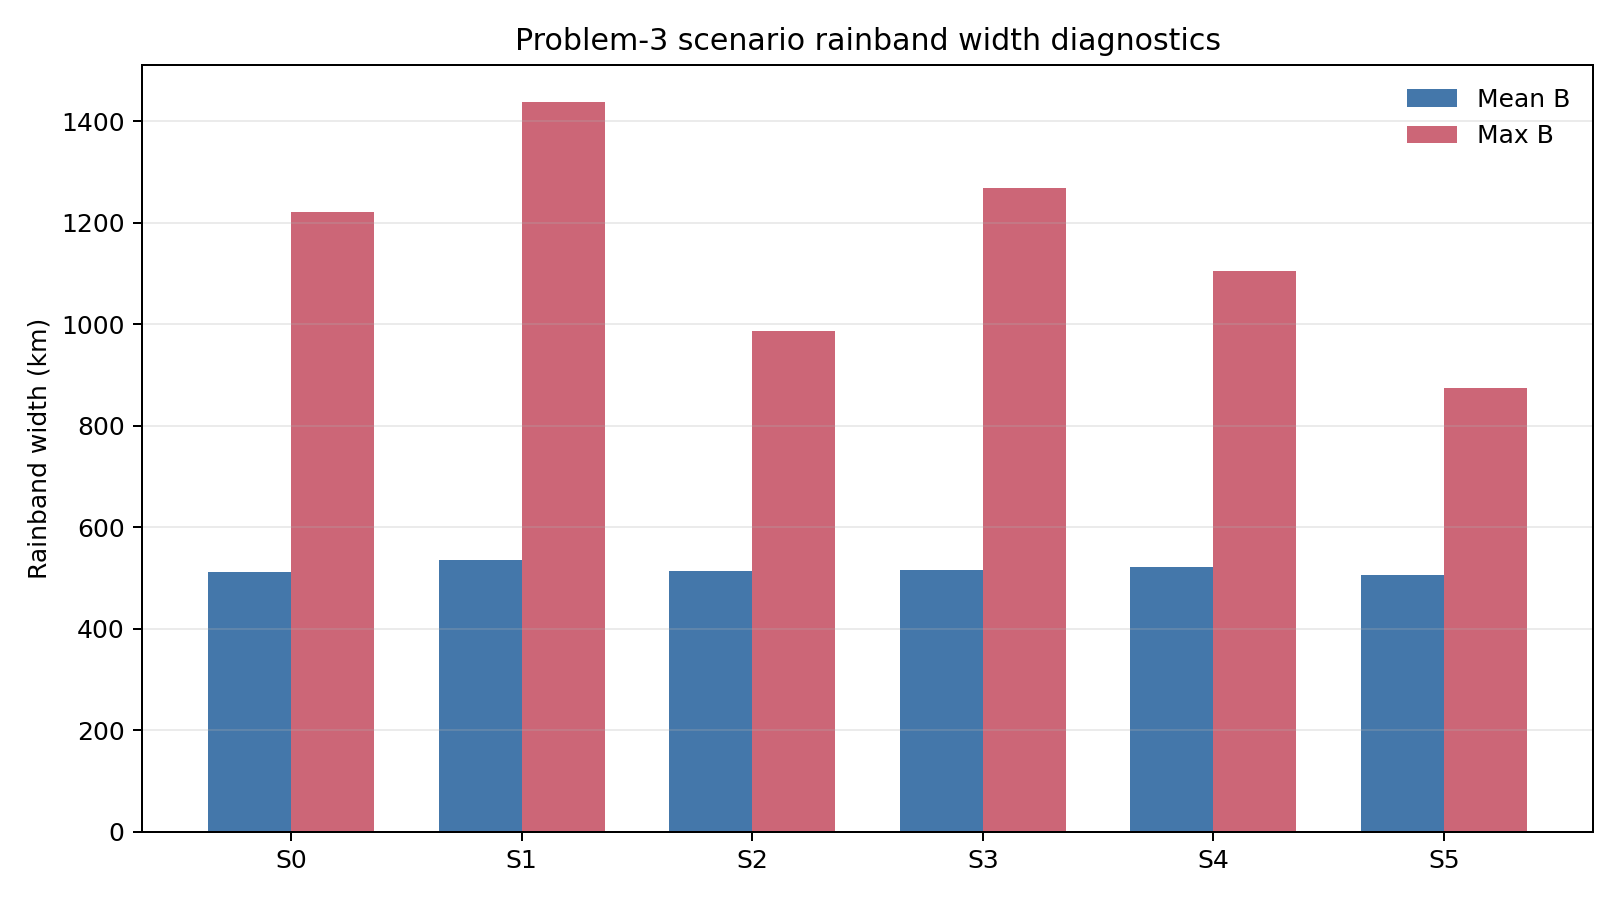
\includegraphics[width=0.78\textwidth]{outputs/figures/problem3/problem3_rainband_width_bars.png}
    \caption{S0--S5 情景生成雨带带宽对比}
    \label{fig:problem3_rainband_width_bars}
\end{figure}

\begin{figure}[H]
  \centering
  \begin{subfigure}{0.48\linewidth}
    \centering
    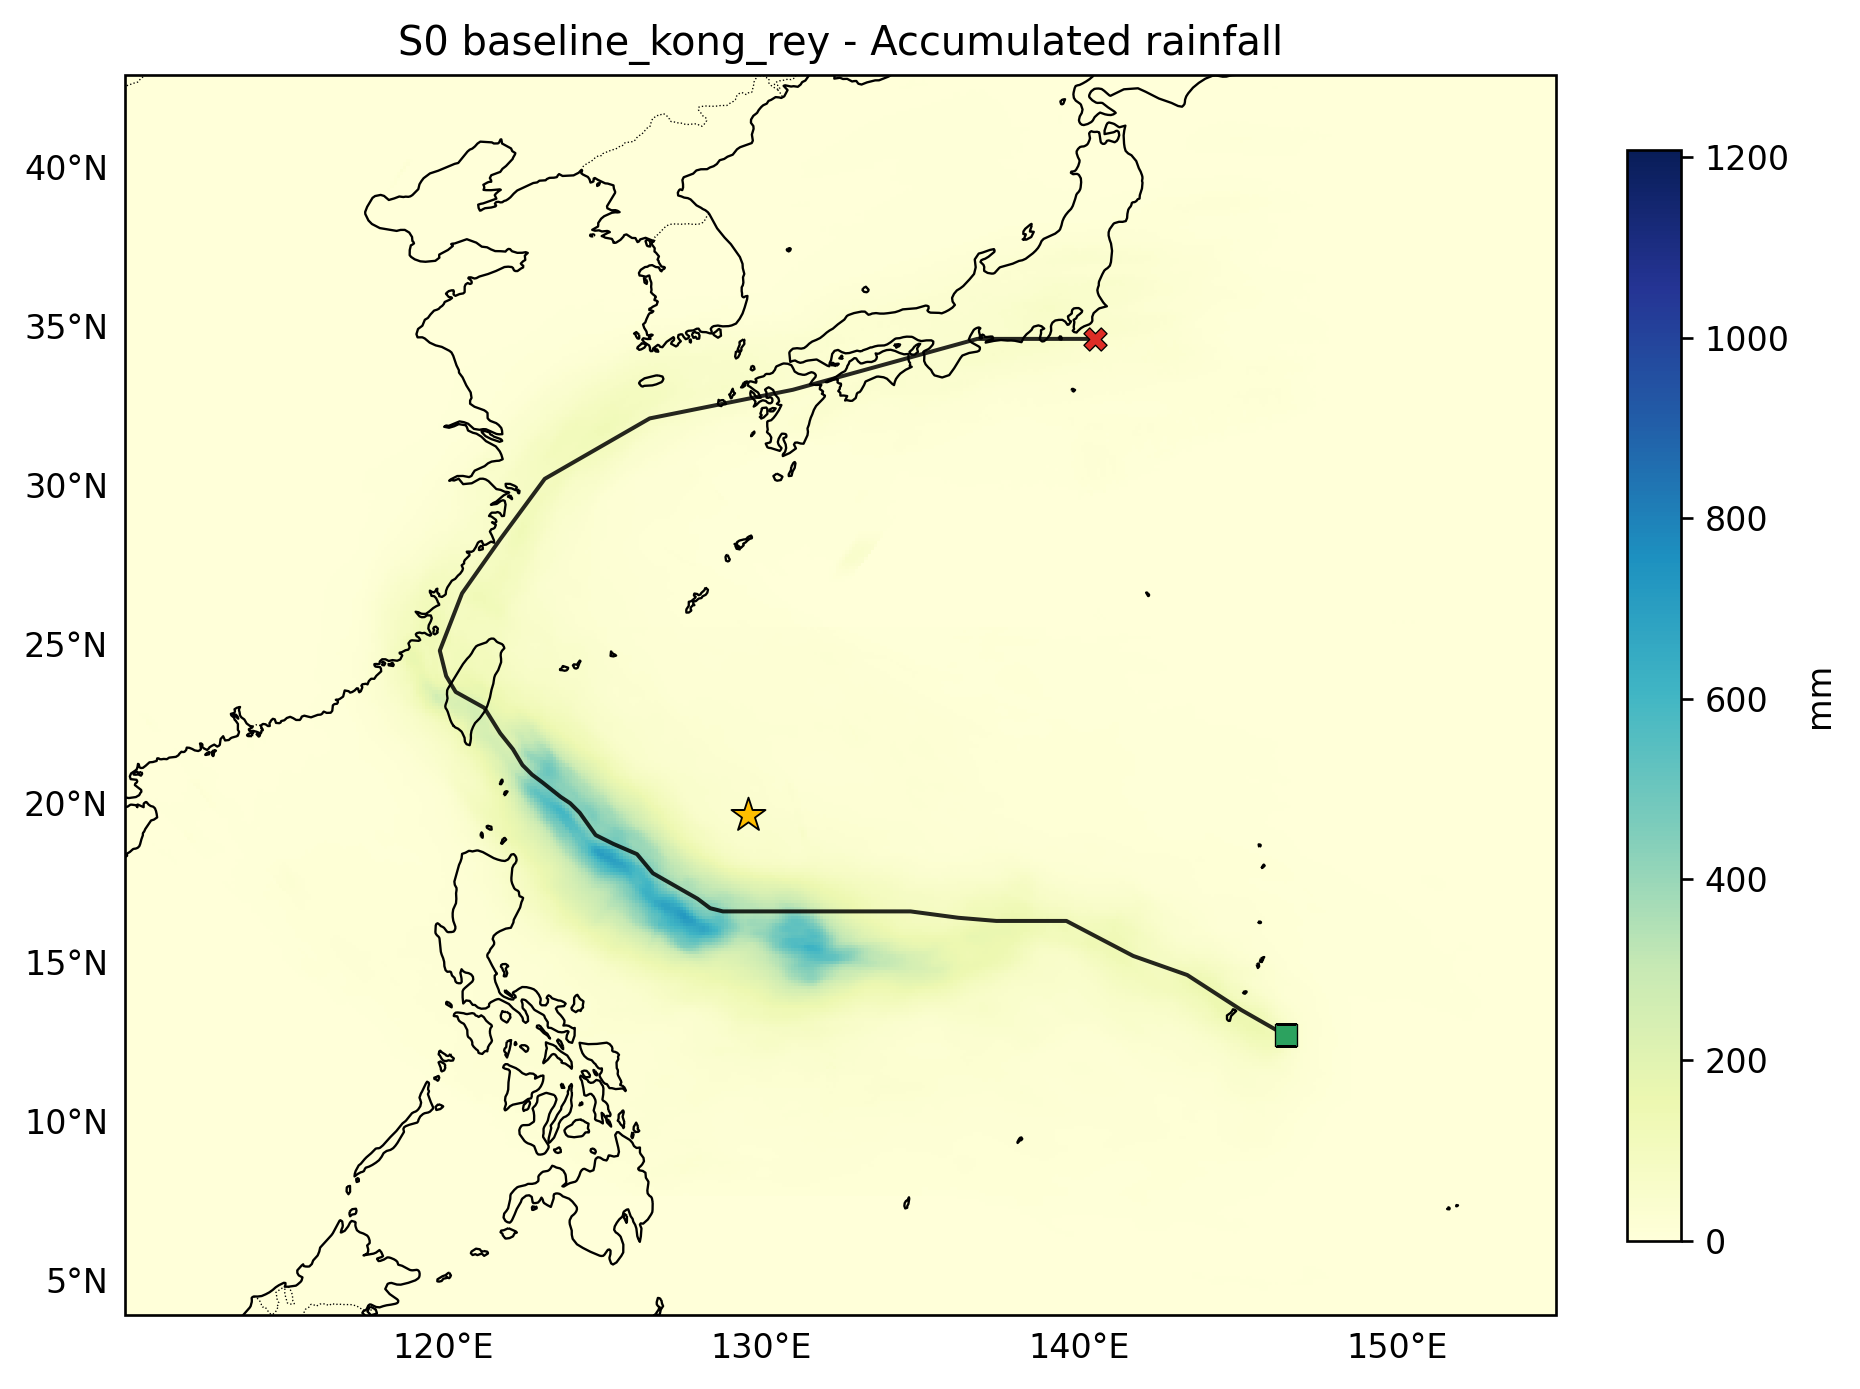
\includegraphics[width=\linewidth]{outputs/figures/problem3/problem3_accum_rain_S0.png}
    \caption{S0 基准情景}
  \end{subfigure}
  \hfill
  \begin{subfigure}{0.48\linewidth}
    \centering
    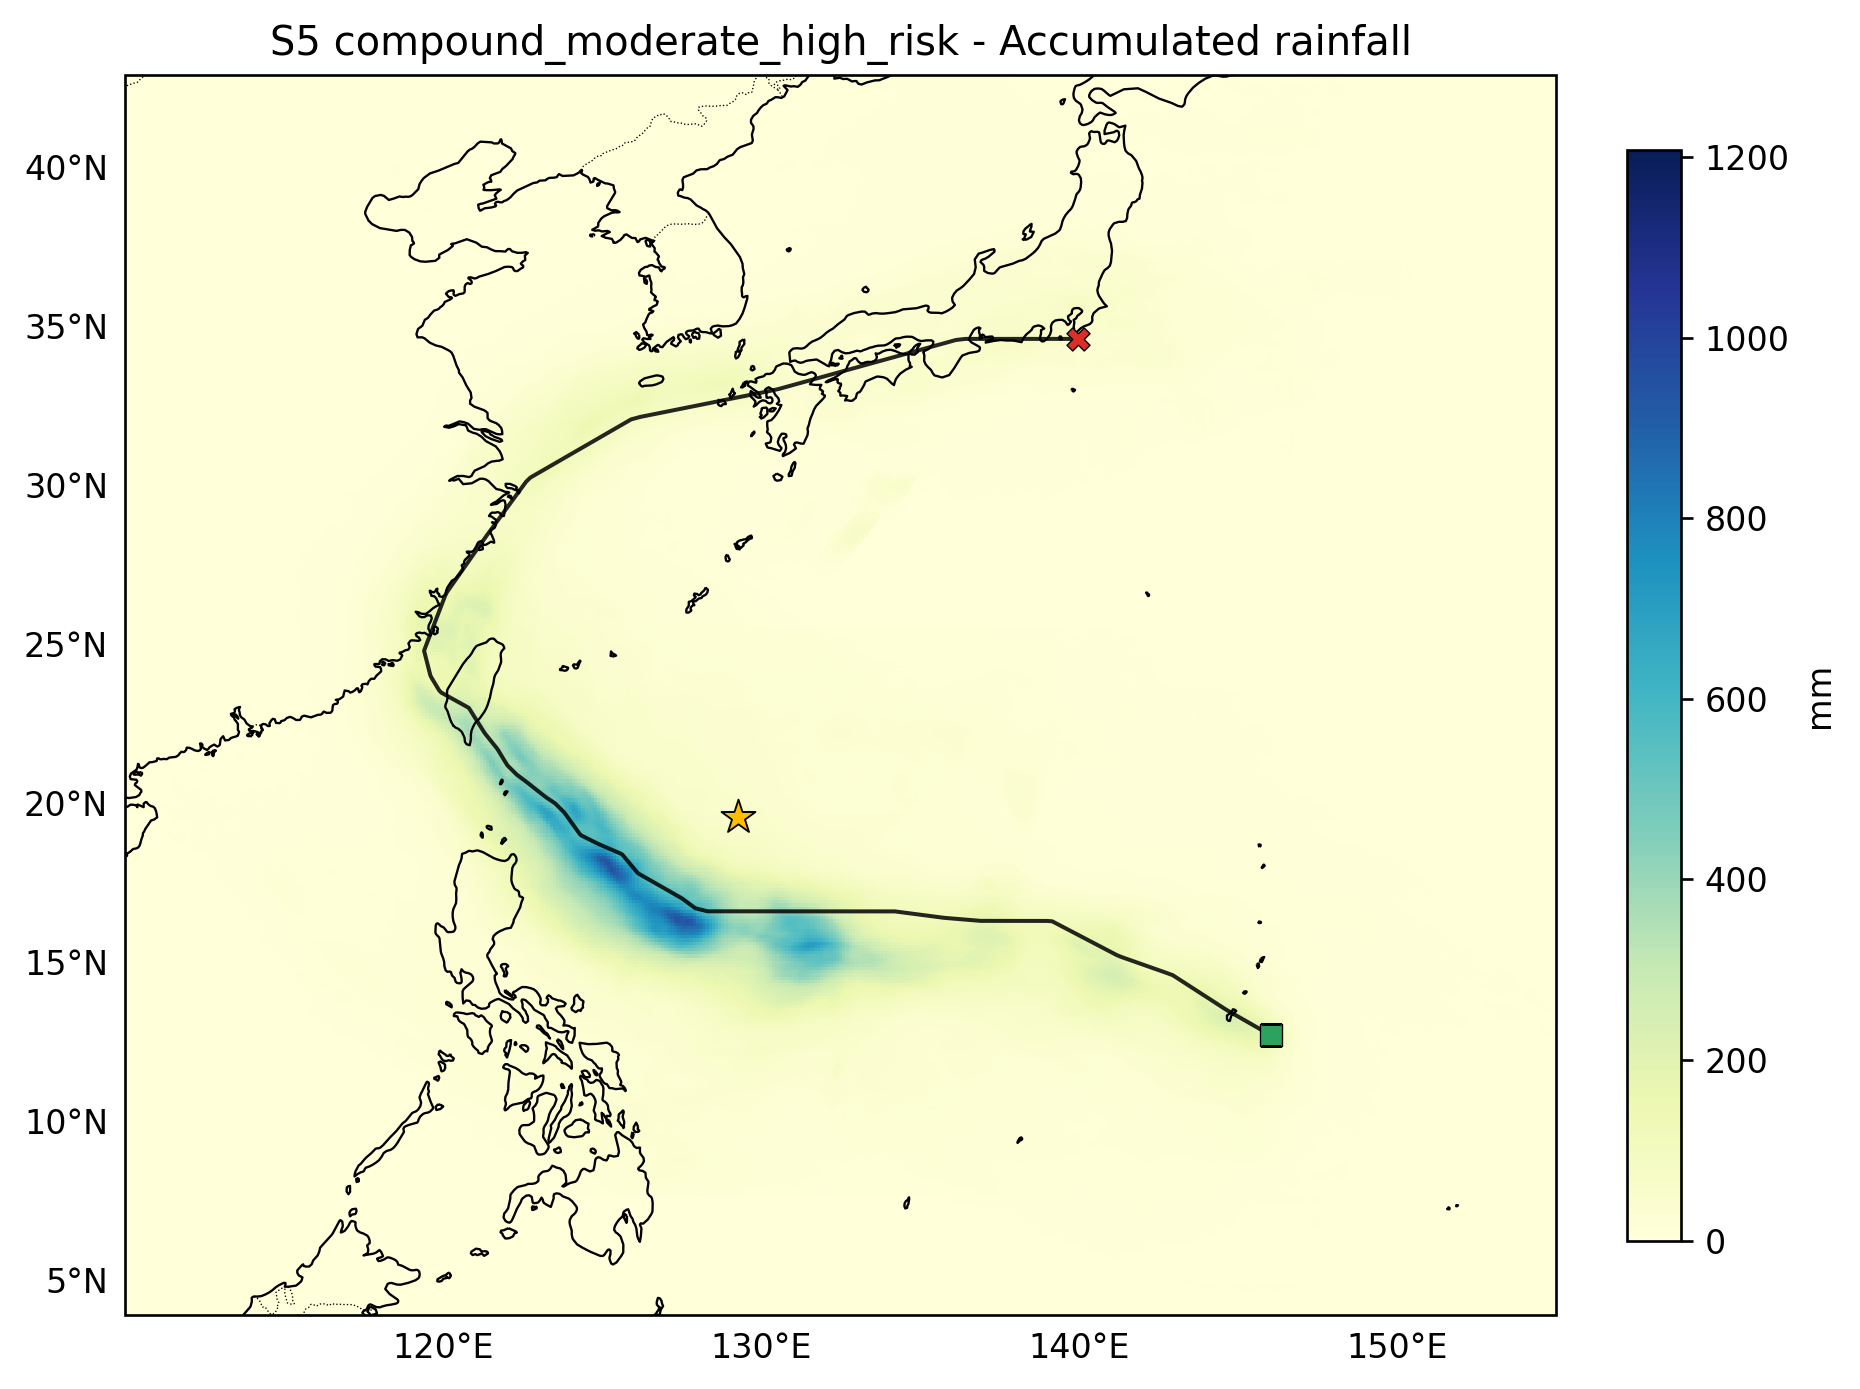
\includegraphics[width=\linewidth]{outputs/figures/problem3/problem3_accum_rain_S5.png}
    \caption{S5 复合高风险情景}
  \end{subfigure}
  \caption{S0 与 S5 固定地理网格事件累计降水对比（单位：mm）}
  \label{fig:problem3_s0_s5_accum}
\end{figure}

\begin{figure}[H]
  \centering
  \begin{subfigure}{0.48\linewidth}
    \centering
    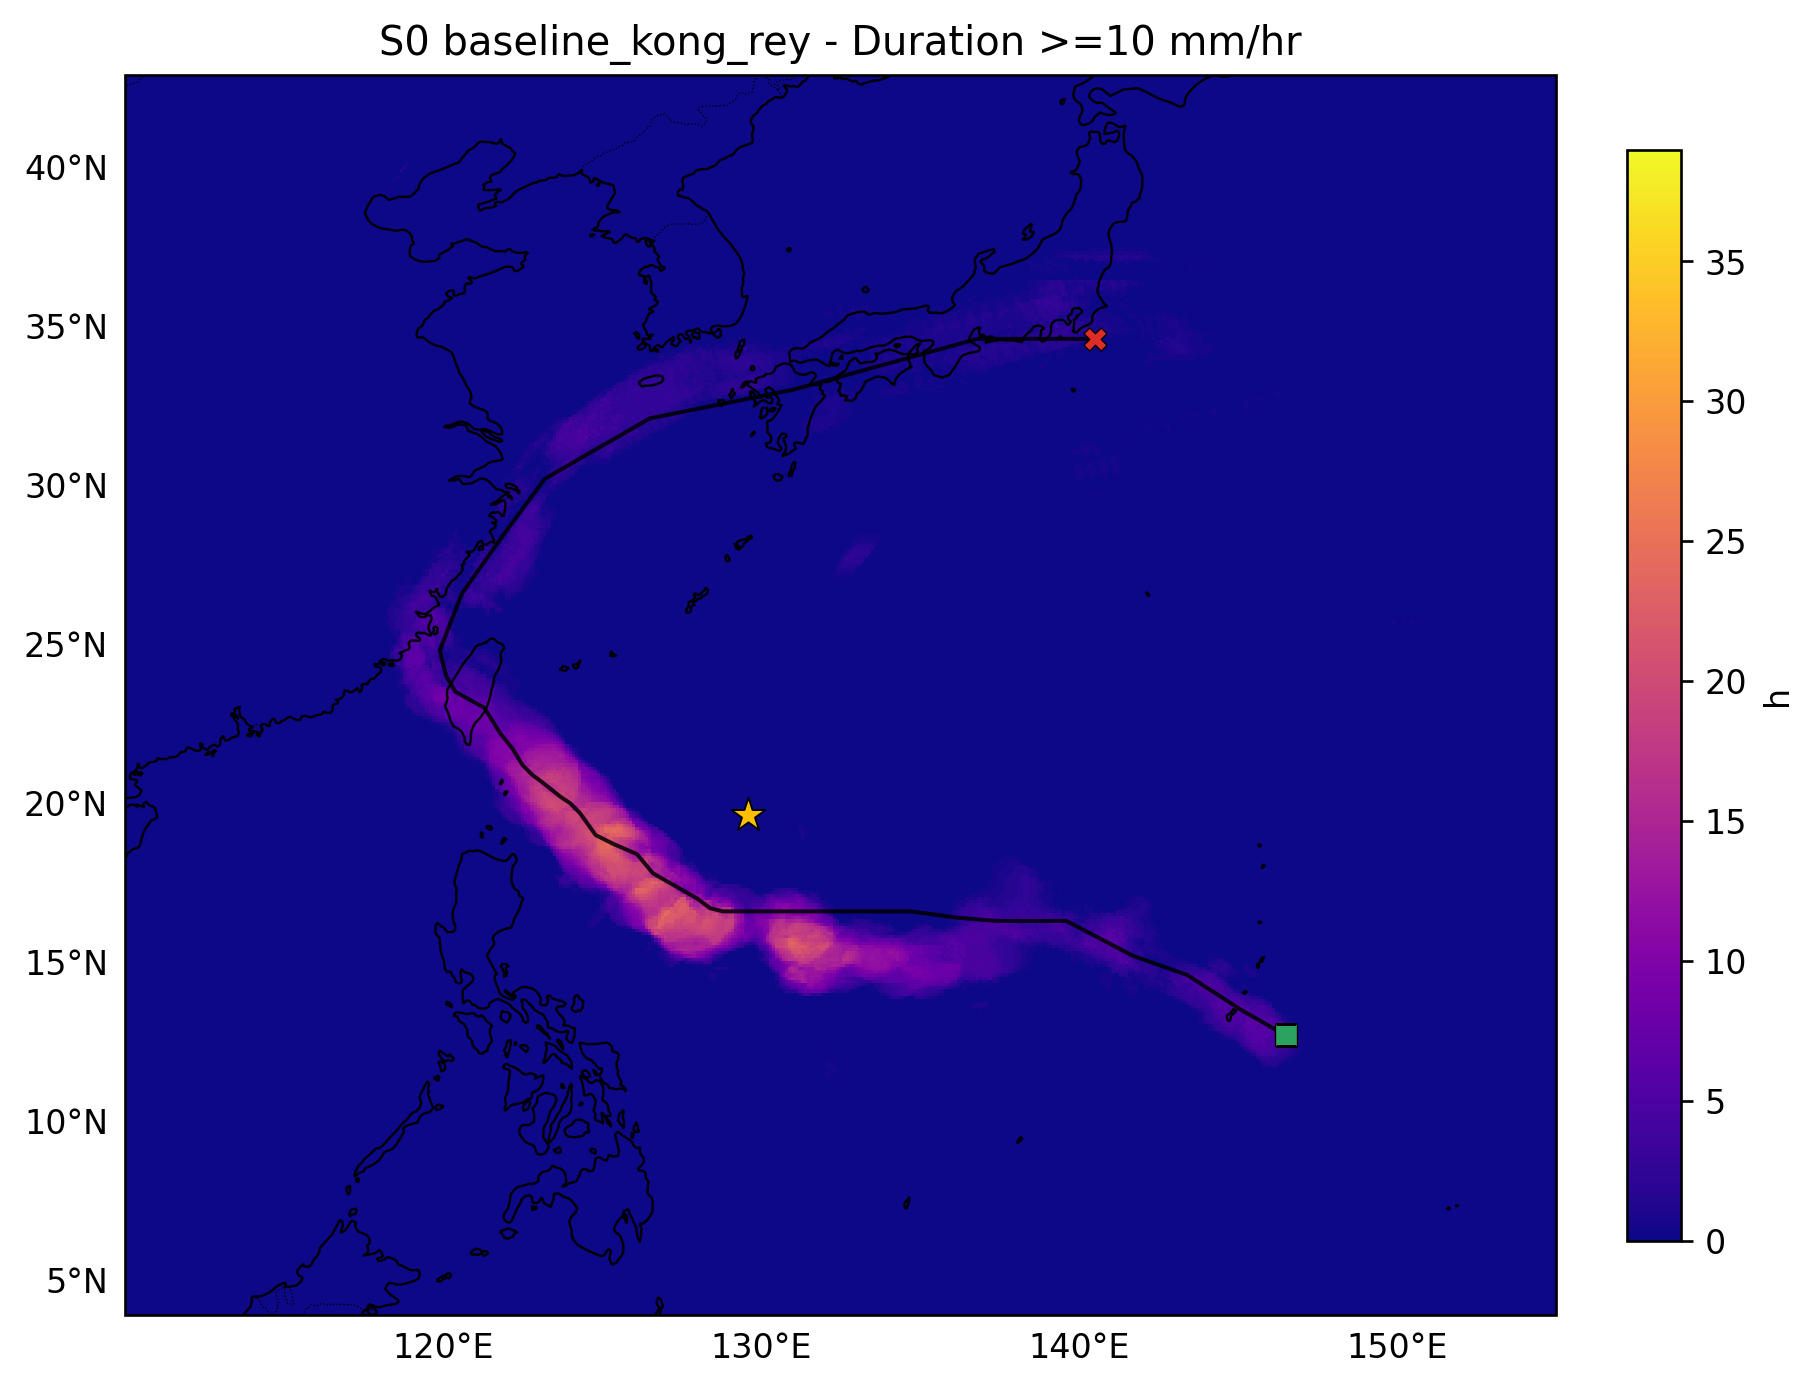
\includegraphics[width=\linewidth]{outputs/figures/problem3/problem3_duration10_S0.png}
    \caption{S0 基准情景}
  \end{subfigure}
  \hfill
  \begin{subfigure}{0.48\linewidth}
    \centering
    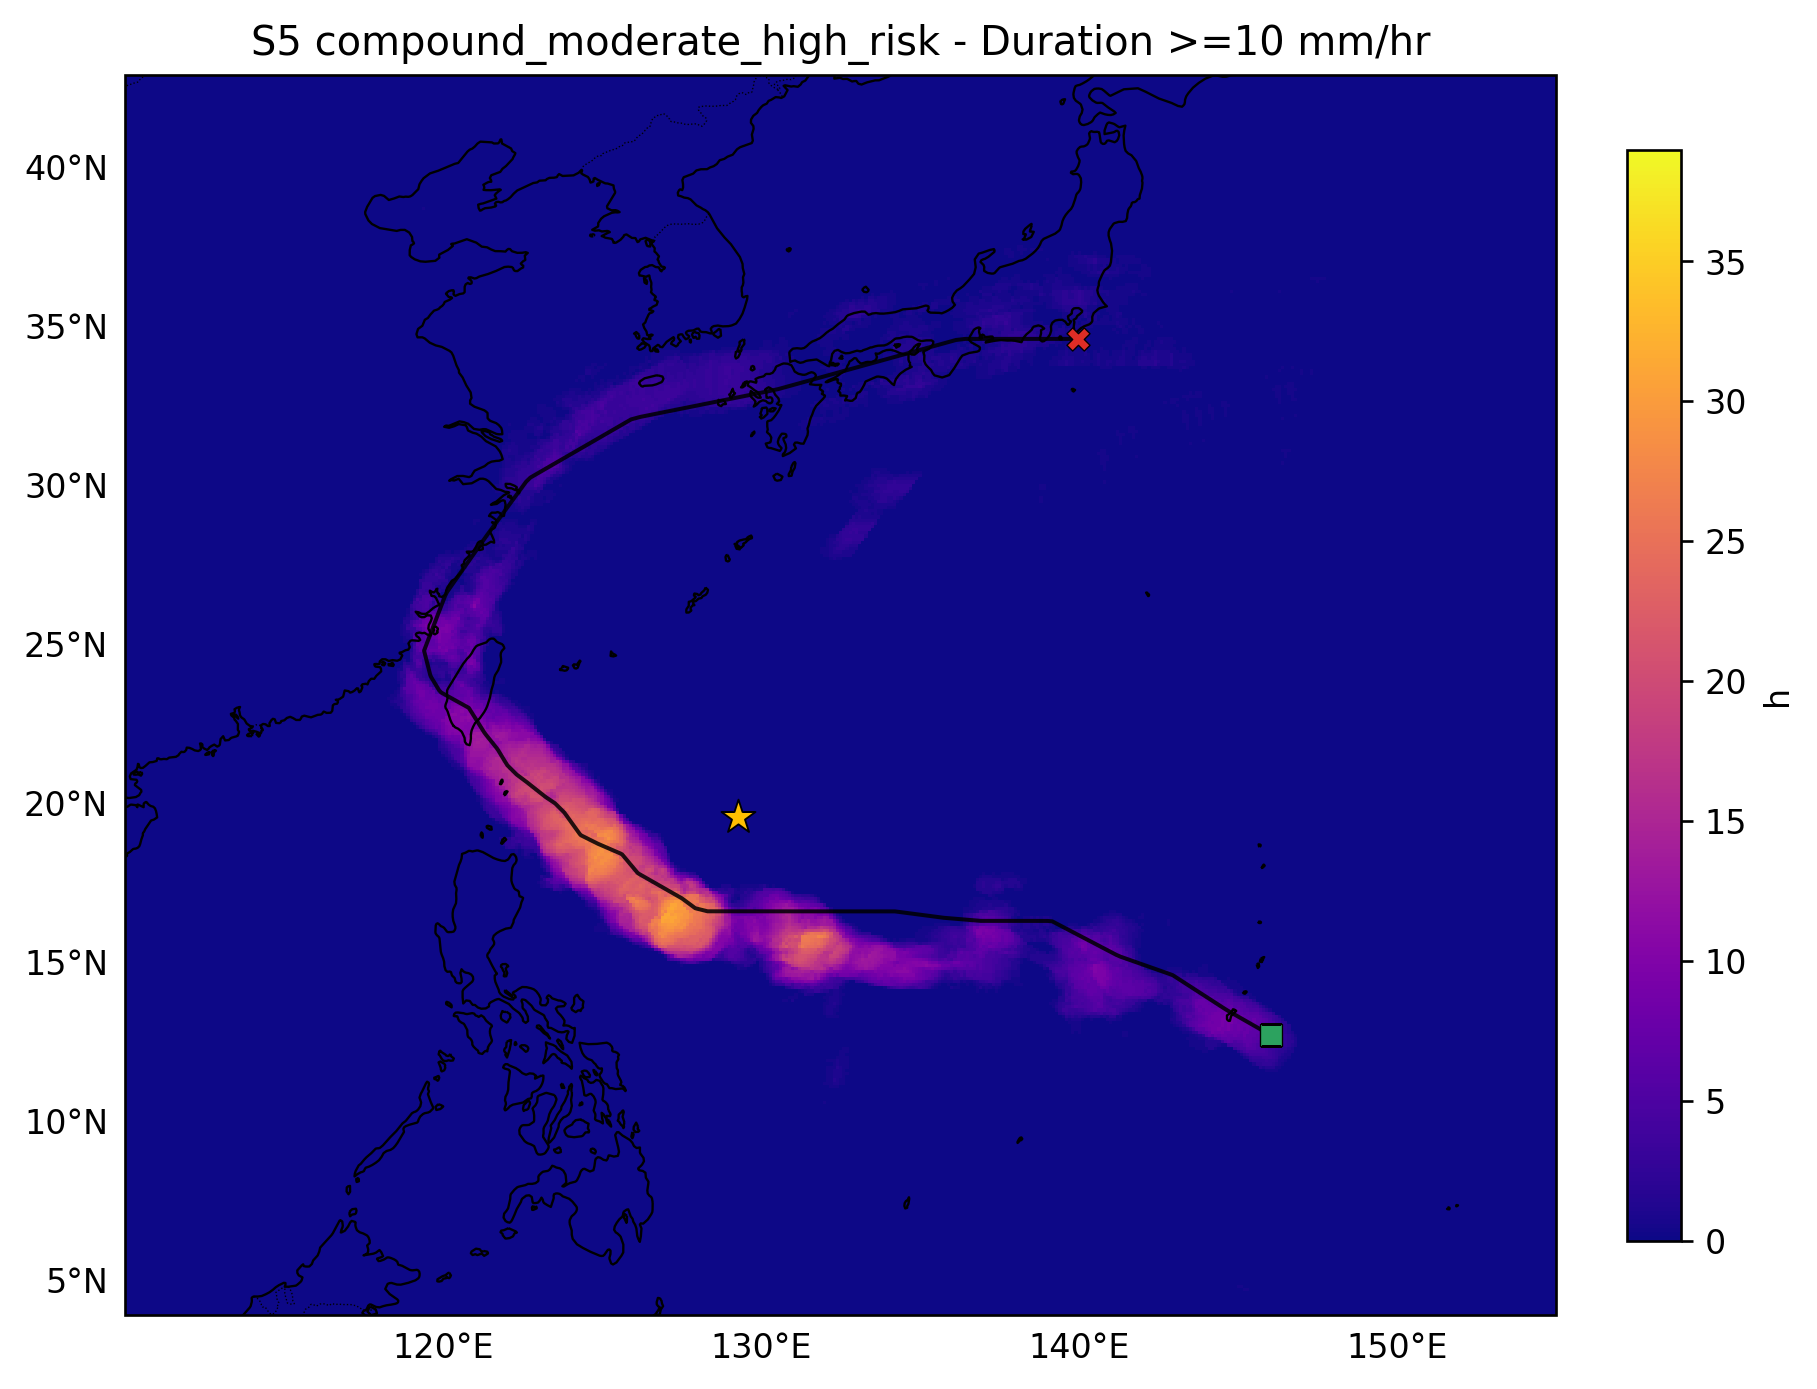
\includegraphics[width=\linewidth]{outputs/figures/problem3/problem3_duration10_S5.png}
    \caption{S5 复合高风险情景}
  \end{subfigure}
  \caption{S0 与 S5 固定地理格点 $D_{10}$ 对比（单位：h）}
  \label{fig:problem3_s0_s5_duration10}
\end{figure}

\begin{figure}[H]
  \centering
  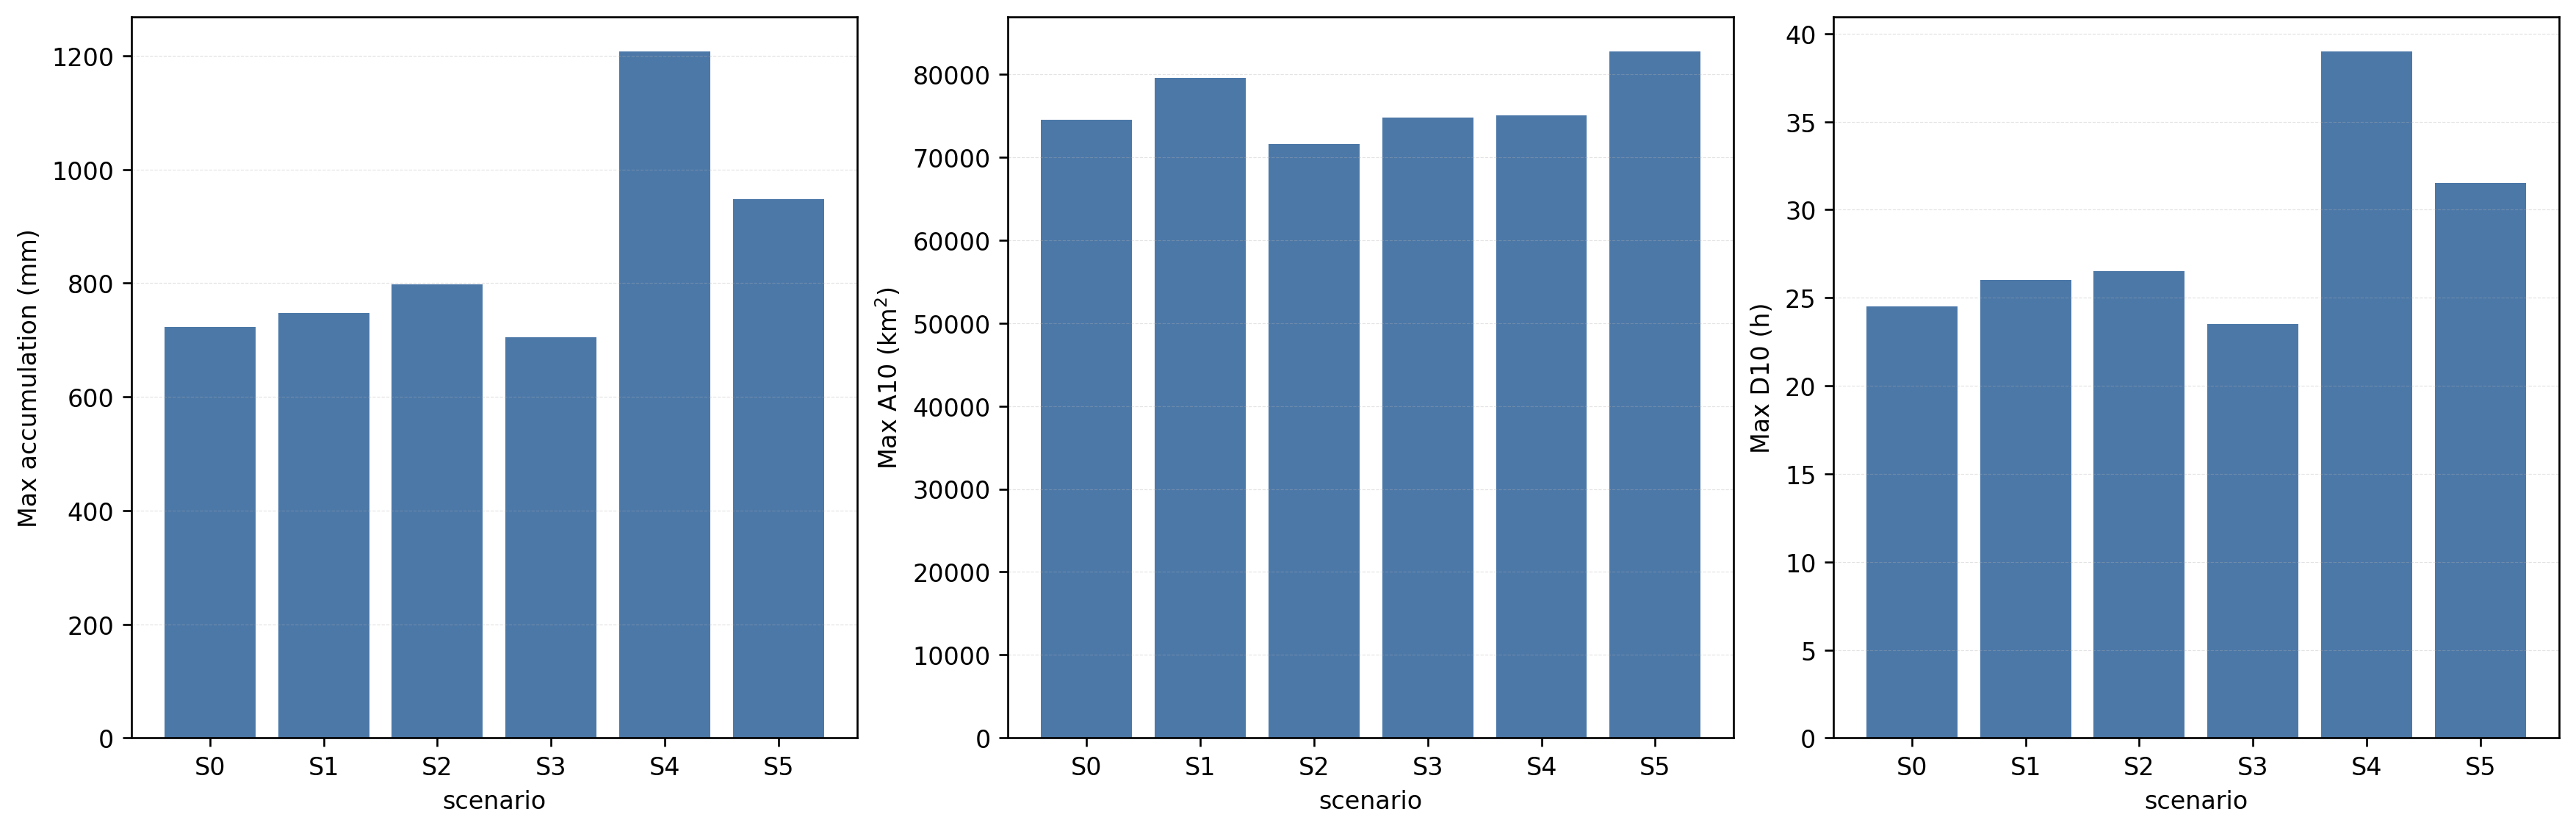
\includegraphics[width=0.92\textwidth]{outputs/figures/problem3/problem3_scenario_metric_bars.png}
  \caption{S0--S5 情景关键降水风险指标对比}
  \label{fig:problem3_metric_bars}
\end{figure}

\begin{figure}[H]
  \centering
  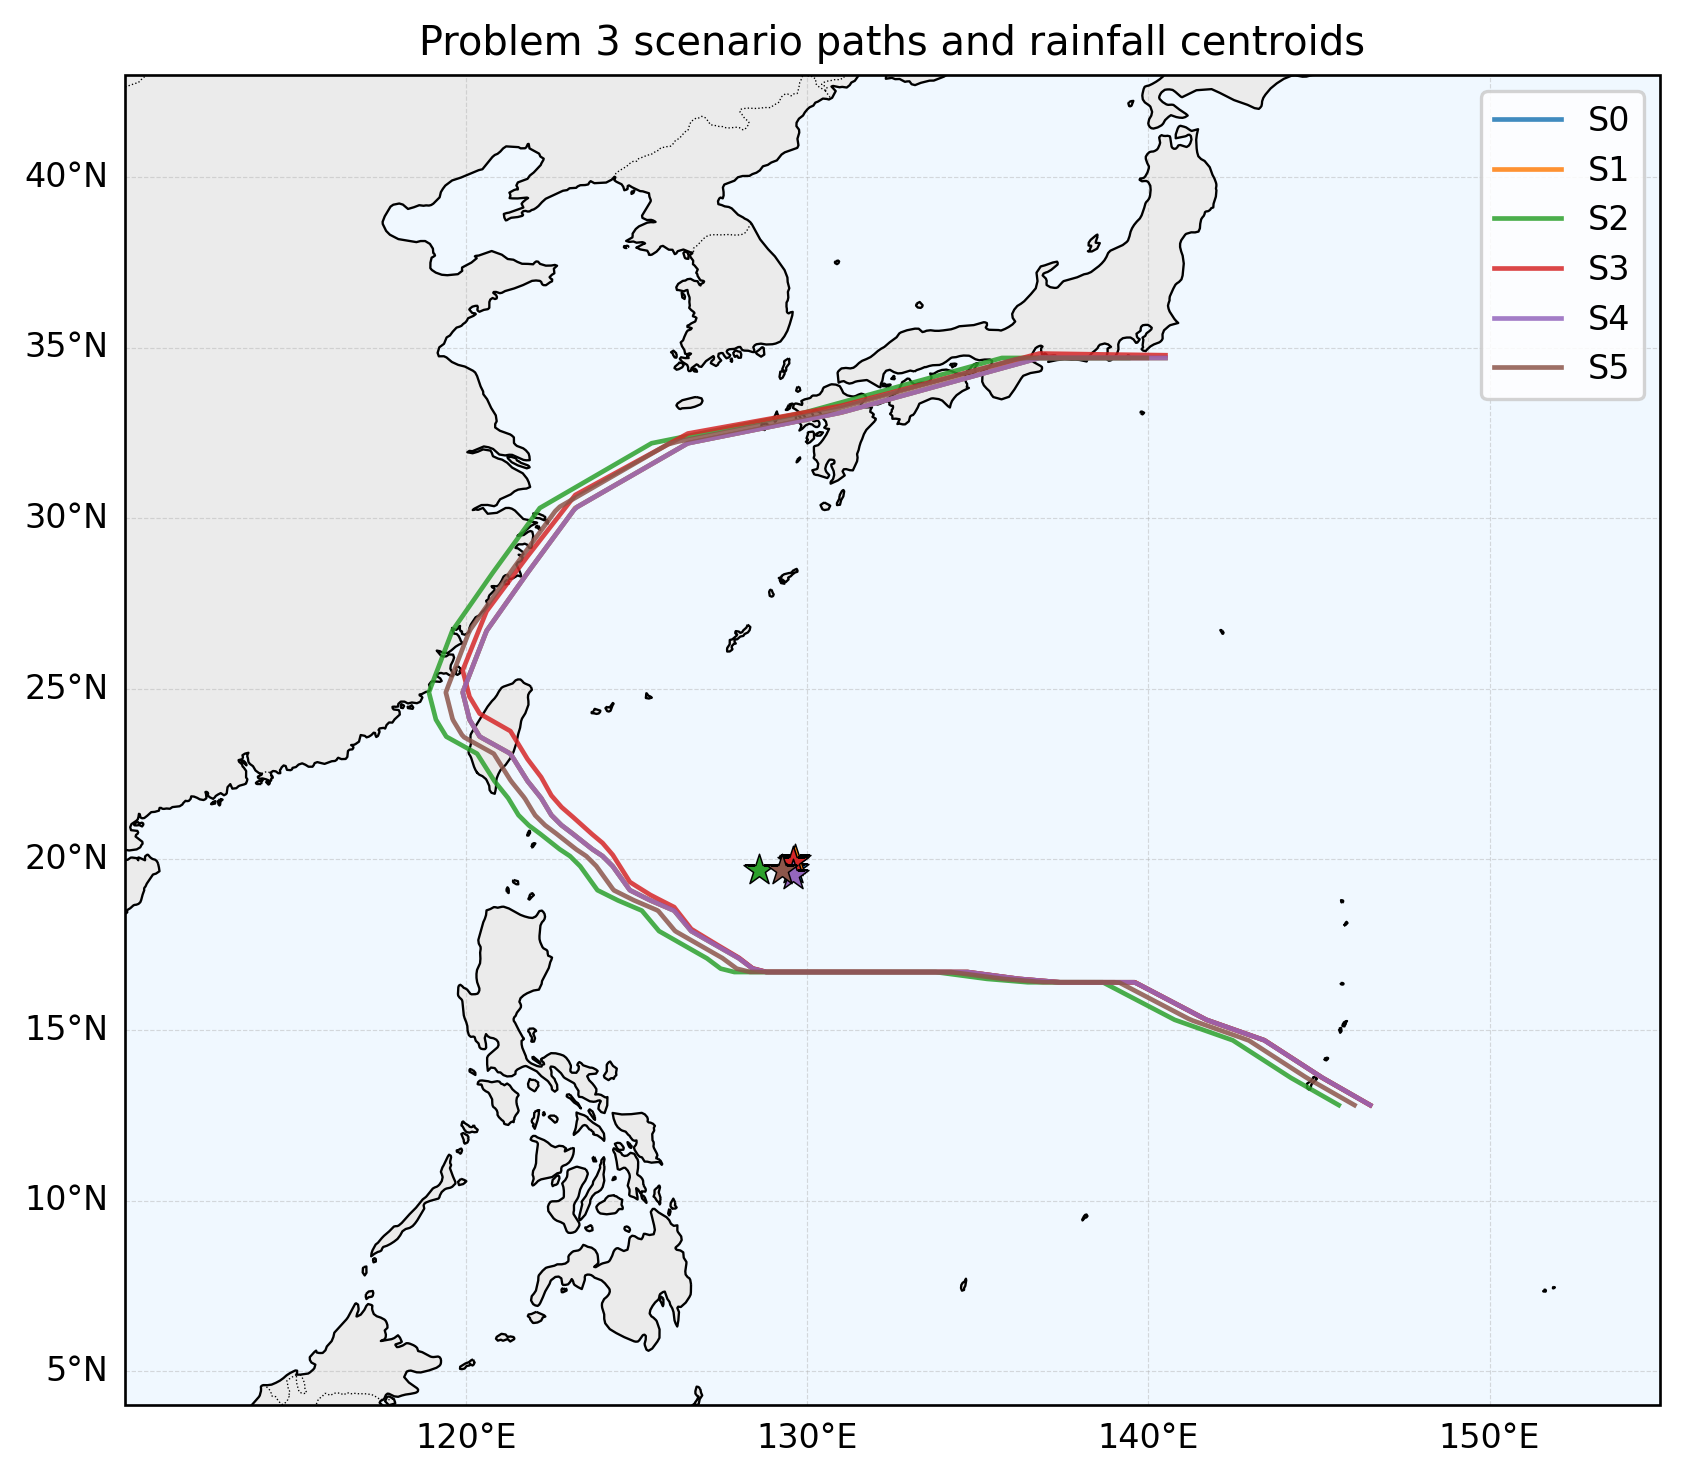
\includegraphics[width=0.86\textwidth]{outputs/figures/problem3/problem3_path_and_centroid_shift.png}
  \caption{S0--S5 路径与事件累计降水质心偏移}
  \label{fig:problem3_path_centroid}
\end{figure}

图~\ref{fig:problem3_s0_s5_accum} 和图~\ref{fig:problem3_s0_s5_duration10} 展示了 S0 与 S5 在固定地理落区上的累计降水和持续时间差异；图~\ref{fig:problem3_metric_bars} 比较了 S0--S5 的关键指标；图~\ref{fig:problem3_path_centroid} 则用于解释路径扰动导致的降水质心偏移。

\subsection{灵敏度分析与物理解释}

强度增强主要影响最大雨强、P99 和强降水面积。路径近岸或西移主要改变累计雨区质心、IoU 和局地落区，因此其影响不一定表现为所有面积指标同步增大。近岸段偏移主要影响沿海风险带的位置，适合用于讨论局地防灾对象的空间转移。移动速度减慢主要影响累计降水和固定地理位置的强降水持续时间，是本组情景中对累计风险最敏感的因子。复合高风险情景表现为最大累计降水、最大强降水面积和持续时间等多项指标同步增加，但并非所有单项指标均达到最大值。

\subsection{小结}

情景实验表明，在历史可比扰动范围内，移动速度减慢是累计降水和持续时间最敏感因子。S4 的最大累计降水相对 S0 增加 $66.98\%$，固定地理格点 $D_{10}$ 最大值增加 $59.18\%$。

强度增强主要扩大强降水范围并增强极端尾部。S1 的最大 $A_{10}$ 增加 $6.70\%$，P99 增加 $3.98\%$，说明强度扰动更直接影响强降水覆盖和雨强尾部。

路径和登陆点变化主要改变风险落区。S2 和 S3 的结果说明，强降水影响区可随路径扰动发生明显空间转移，因此防灾减灾中不能只关注总雨量大小，还应关注降水落区的变化。

\section{模型检验与灵敏度分析}

\subsection{模型有效性检验}
本文从数据对齐、历史伪缺失验证、消融实验和情景一致性四个层面检验模型。问题一中，33420 个 GPM 半小时时次均完成路径匹配，中心误差均值为 $0.331\ \mathrm{km}$、最大误差为 $0.785\ \mathrm{km}$，说明路径插值与 GPM 文件中心高度一致。增强随机森林对 P95 降水强度、强降水等效半径、降水质心偏移和雨带各向异性的测试集 $R^2$ 均超过 $0.64$，表明路径、强度、移动、海陆、地形和季节背景能够解释台风降水空间结构的主要变化。

问题二采用历史台风伪缺失验证。相较 initial 场，calibrated 场使 P95 误差降低 $39.73\%$，P99 误差降低 $39.41\%$，$10\ \mathrm{mm/hr}$ 强降水面积误差降低 $37.13\%$，CSI10 从 $0.0230$ 提升至 $0.1097$，F1\_10 从 $0.0390$ 提升至 $0.1773$。这说明极端分位数校准能够明显改善极端降水强度和强降水区域识别能力。环境变量消融实验显示，Base-old、Env-full 和 Env-key 三组设置整体差异较小，最终选择更稳定的 Base-old 作为问题二相似检索环境距离设置。

问题三对生成雨场进行了质量检查。S0--S5 共生成 $(2841,201,201)$ 的半小时雨强场，NaN、Inf、负值和全零场数量均为 $0$。S0 的最大累计降水为 $723.48\ \mathrm{mm}$，与问题二 KONG-REY 地理基准结果 $722.05\ \mathrm{mm}$ 接近，因此可作为情景比较的内部对照。

\subsection{灵敏度分析}
问题二对 Top-$K$ 相似样本数量、强度权重、移动权重、环境权重和 EOF/PCA 融合系数进行了参数敏感性检验。结果显示，不同参数设置下 P95 误差、P99 误差、强降水面积误差和 CSI10 均未出现突变，说明生成模型对关键超参数具有一定鲁棒性。其中，$K=20$ 在历史模板多样性和样本相似性之间取得折中。

问题三情景实验表明，在历史可比扰动范围内，移动速度减慢是累计降水和持续时间最敏感因子；强度增强主要扩大强降水范围并增强极端尾部；路径和登陆点变化主要改变风险落区。这一结果说明，未来台风极端降水风险不仅取决于台风强度，也取决于移动速度和路径相对陆地的位置。

\section{结论与最终答案汇总}

\begin{table}[H]
  \centering
  \caption{各问题最终答案汇总}
  \begin{tabularx}{\linewidth}{lXX}
    \toprule
    问题 & 最终结果 & 说明 \\
    \midrule
    问题一 & 构建了降水强度、强降水面积、质心偏移、非对称性、雨带各向异性和降水带宽等指标，并用相关性分析和随机森林解释路径、强度、移动及环境因素影响 & 台风强度主控降水强度和范围，移动方向与移动速度显著影响非对称结构和雨带横向扩展；海陆覆盖和地形起伏具有非线性调制作用 \\
    问题二 & 生成了 KONG-REY 和 MAN-YI 的可能半小时降水时空分布 & KONG-REY 地理累计降水峰值为 $722.047\ \mathrm{mm}$，MAN-YI 地理累计降水峰值为 $533.592\ \mathrm{mm}$；两场台风均呈现移动方向左前侧主雨象限特征 \\
    问题三 & 构造 S0--S5 虚拟台风情景，比较路径偏移、强度增强、移动减慢和复合扰动对降水风险的影响 & S4 移动减慢使最大累计降水相对 S0 增加 $66.98\%$、$D_{10}$ 最大值增加 $59.18\%$；S5 复合扰动使多个风险指标同步放大 \\
    \bottomrule
  \end{tabularx}
\end{table}

\section{模型评价与改进方向}

\subsection{模型优点}
\begin{enumerate}
  \item \textbf{可解释性较强。}

  本文围绕“路径--强度--移动--环境--降水结构”建立模型，不仅给出降水生成结果，也能解释强度、移动方向、近岸环境和地形条件对降水强度、范围与偏向的影响。

  \item \textbf{避免了目标台风降水信息泄漏。}

  对于 KONG-REY 和 MAN-YI，模型只使用路径、强度、移动、时间和近岸环境等安全变量，不使用真实降水派生指标，因此问题二的生成结果具有外推意义。

  \item \textbf{能较好保留真实台风降水结构。}

  模型采用相似历史时次和真实 GPM 降水模板进行迁移生成，并结合结构修正和极端分位数校准，兼顾了空间形态和极端降水特征。GPM IMERG 本身具有半小时降水估计能力，适合作为本文历史降水模板来源\cite{ref2}。
\end{enumerate}

\subsection{模型不足}
\begin{enumerate}
  \item \textbf{动态气象环境变量仍不充分。}

  台风降水还受水汽输送、垂直风切变、海温和大尺度环流等因素影响，本文主要依靠历史模板和海陆地形变量间接刻画，因而对特殊环流背景下的异常降水解释仍有限。

  \item \textbf{相对坐标转换可能削弱固定地形作用。}

  将历史降水模板旋转到台风相对运动坐标系，有利于对齐雨带结构，但也可能使山脉、海岸线等固定地理强迫被一并“旋转”，从而弱化真实地形对局地强降水落区的锁定作用。

  问题三情景比较采用统一生成链条下的 S0 作为内部对照，侧重分析扰动情景相对基准的变化；不同网格设置下的逐像元落区仍存在一定离散化差异。
\end{enumerate}

\subsection{改进方向}
未来可以引入更长时段的多源降水资料、再分析环流场、垂直风切变和水汽通量等环境变量，并进一步结合物理约束生成模型或区域数值模式输出，提高复杂地形和登陆台风降水模拟能力。

\phantomsection
\addcontentsline{toc}{section}{参考文献}
\begin{thebibliography}{99}
  \bibitem{ref1} Ying M, Zhang W, Yu H, Lu X, Feng J, Fan Y, et al. An overview of the China Meteorological Administration tropical cyclone database[J]. Journal of Atmospheric and Oceanic Technology, 2014, 31(2): 287-301.
  \bibitem{ref2} NASA. IMERG: Integrated Multi-satellitE Retrievals for GPM[EB/OL]. NASA Global Precipitation Measurement Mission.
  \bibitem{ref3} MacFerrin M, et al. The Earth Topography 2022 (ETOPO 2022) global DEM dataset[J]. Earth System Science Data, 2025, 17: 1835-1849.
  \bibitem{ref4} Natural Earth. 1:50m Physical Vectors: Land polygons[DB/OL]. Natural Earth.
  \bibitem{ref5} Lorenz E N. Atmospheric predictability as revealed by naturally occurring analogues[J]. Journal of the Atmospheric Sciences, 1969, 26(4): 636-646.
  \bibitem{ref6} Horton P. AtmoSwing: Analog Technique Model for Statistical Weather Forecasting[J]. Geoscientific Model Development, 2019, 12: 2915-2940.
  \bibitem{ref7} Breiman L. Random Forests[J]. Machine Learning, 2001, 45: 5-32.
  \bibitem{ref8} 陈爱军, 吴雪菲, 楚志刚. 精细化评估GPM/IMERG产品对台风“妮坦”降水的观测精度[J]. 气象科学, 2021, 41(5): 678-686.
  \bibitem{ref9} 韩芙蓉, 鹿翔, 吴天贻, 徐业佳, 韩兴, 蔡晓冬. 多卫星融合降水产品对2015—2020年登陆浙江台风降水的监测能力评估[J]. 暴雨灾害, 2023, 42(1): 57-66.
  \bibitem{ref10} 徐{\songtifallback 燚}, 钱浩, 罗玲, 余晖. 基于ECMWF模式预报的台风降水地形订正方法[J]. 气象学报, 2019, 77(4): 674-685.
  \bibitem{ref11} 高延康, 赵铜铁钢, 田雨, 杨芳, 郑飞飞, 陈晓宏. 台风活动对中国沿海地区极端降水的影响[J]. 水科学进展, 2023, 34(1): 1-11.
  \bibitem{ref12} 黄燕燕, 蒙伟光, 冯业荣, 张诚忠, 陈德辉, 郑彬. 华南登陆台风降水不对称性及持续性问题[J]. 气象, 2023, 49(4): 385-399.
  \bibitem{ref13} Liu C C, et al. The influence of terrain on the tropical rainfall potential technique in Taiwan[J]. Weather and Forecasting, 2009, 24(3): 785-799.
  \bibitem{ref14} IPCC. Climate Change 2021: The Physical Science Basis, Chapter 11: Weather and Climate Extreme Events[R]. Cambridge University Press, 2021.
  \bibitem{ref15} NOAA Geophysical Fluid Dynamics Laboratory. Global Warming and Hurricanes[EB/OL].
\end{thebibliography}

\appendix

\section{支撑材料文件列表}
\begin{table}[H]
  \centering
  \caption{支撑材料文件列表}
  \begin{tabularx}{\linewidth}{lXX}
    \toprule
    文件类别 & 文件名称 & 内容说明 \\
    \midrule
    原始数据 & \texttt{CMABSTdata} & 台风路径资料，包括台风编号、名称、中心位置、中心气压、最大风速等字段 \\
    原始数据 & \texttt{GPM\_3IMERGHHE.07} & GPM 半小时降水空间分布图 \\
    外部数据 & \texttt{Natural Earth land polygons} & 用于构造海陆覆盖比例和陆地判定变量 \\
    外部数据 & \texttt{ETOPO 2022} & 用于构造地形高程、地形起伏等环境变量 \\
    中间数据 & \texttt{historical library index} & 历史台风半小时样本索引及路径、强度、环境特征 \\
    中间数据 & \texttt{target typhoon inputs} & KONG-REY 和 MAN-YI 的安全输入特征表 \\
    结果文件 & \texttt{problem1 result tables} & 问题一相关性、随机森林重要性和分组验证结果 \\
    结果文件 & \texttt{problem1 rainband width tables} & 历史样本雨带带宽统计、随机森林指标和重要性结果 \\
    结果文件 & \texttt{problem2 generated fields} & 问题二目标台风生成降水场 \\
    结果文件 & \texttt{problem2/problem3 rainband width diagnostics} & 目标台风和 S0--S5 情景生成雨带带宽诊断表与图 \\
    结果文件 & \texttt{validation result tables} & 伪缺失验证、消融实验和模型对比结果 \\
    图像文件 & \texttt{figures} & 路径图、降水分布图、重要性图、验证图和最终结果图 \\
    \bottomrule
  \end{tabularx}
\end{table}

\section{源程序代码说明}
本文程序主要使用 Python 编写，按数据预处理、问题一分析、问题二生成和结果验证四类组织。

第一类为数据预处理程序，用于读取 CMABST 台风路径资料和 GPM 降水图像，完成时间对齐、路径插值、降水场裁剪和基础特征提取。第二类为问题一分析程序，用于计算降水强度、强降水面积、质心偏移、雨带形态、象限贡献和降水带宽等指标，并完成相关性分析、随机森林特征重要性分析和分组验证。第三类为问题二生成程序，用于构造目标台风安全输入表，检索 Top-K 相似历史时次，完成历史模板迁移、EOF/PCA 结构修正和极端分位数校准，最终输出 KONG-REY 和 MAN-YI 的可能降水场。第四类为结果汇总和检验程序，用于整理目标台风生成结果、伪缺失验证结果、环境变量消融实验结果、雨带带宽诊断和论文图表。所有程序均由团队在本地运行，论文中使用的表格和图像均来自程序实际输出。

\subsection*{问题一核心代码}
问题一核心程序位于 \path{scripts/10_problem1_analysis_enhanced.py}。雨带带宽特征由 \path{scripts/32_add_rainband_width_features.py} 和 \path{scripts/rainband_width_utils.py} 计算后并入最终历史样本表。该部分对降水结构指标与路径、强度、移动、海陆和地形变量进行随机森林解释，并用置换重要性识别主要影响因素。

\begin{lstlisting}[language=Python,caption={问题一核心代码：随机森林解释模型与置换重要性}]
rf_targets = [
    "rain_max",
    "rain_p95",
    "rain_area_10_km2",
    "rain_area_10_equiv_radius_km",
    "centroid_offset_km",
    "anisotropy",
    "rainband_width_km",
]
rf_targets = [c for c in rf_targets if c in model_df.columns]

importance_records = []
metric_records = []

for target in rf_targets:
    sub = model_df[x_cols + [target]].dropna().copy()
    if len(sub) < 100:
        continue

    X = sub[x_cols]
    y = sub[target]
    X_train, X_test, y_train, y_test = train_test_split(
        X, y, test_size=0.25, random_state=42
    )

    rf = RandomForestRegressor(
        n_estimators=250,
        max_depth=14,
        min_samples_leaf=20,
        random_state=42,
        n_jobs=-1,
    )
    rf.fit(X_train, y_train)

    pred_train = rf.predict(X_train)
    pred_test = rf.predict(X_test)
    metric_records.append(
        {
            "target": target,
            "n_train": len(X_train),
            "n_test": len(X_test),
            "train_r2": rf.score(X_train, y_train),
            "test_r2": rf.score(X_test, y_test),
            "train_mae": mean_absolute_error(y_train, pred_train),
            "test_mae": mean_absolute_error(y_test, pred_test),
            "train_rmse": mean_squared_error(y_train, pred_train) ** 0.5,
            "test_rmse": mean_squared_error(y_test, pred_test) ** 0.5,
        }
    )

    result = permutation_importance(
        rf, X_test, y_test, n_repeats=10, random_state=42, n_jobs=1
    )
    imp = pd.DataFrame(
        {
            "target": target,
            "feature": x_cols,
            "importance_mean": result.importances_mean,
            "importance_std": result.importances_std,
        }
    ).sort_values("importance_mean", ascending=False)
    importance_records.append(imp)
\end{lstlisting}

\subsection*{问题二核心代码}
问题二核心程序主要位于 18、19 和 21 号脚本。其主线是：安全特征检索 Top-K 历史相似时次、在台风相对运动坐标系下融合历史模板，再进行极端分位数校准。生成结果的雨带带宽诊断由 \path{scripts/33_problem2_rainband_width_diagnostics.py} 计算，不参与安全输入构造。

\begin{lstlisting}[language=Python,caption={问题二核心代码：安全相似检索、模板融合与极端校准}]
SAFE_FEATURE_COMPONENTS = {
    "track": ["lat", "lon_180"],
    "intensity": ["WND", "PRES", "intensity"],
    "motion": [
        "move_speed_kmh", "move_dir_sin", "move_dir_cos",
        "wind_change_rate", "pressure_change_rate",
    ],
    "environment": ["is_land", "signed_coast_dist_km", "coast_dist_km"],
    "time": ["month_sin", "month_cos"],
    "life_progress": ["life_progress"],
}

def compute_component_distances(target_z, history_z, component_indices):
    components = {}
    total = np.zeros(history_z.shape[0], dtype=np.float64)
    for component, indices in component_indices.items():
        if not indices:
            components[component] = np.zeros(history_z.shape[0])
            continue
        diff = history_z[:, indices] - target_z[np.newaxis, indices]
        comp_dist = np.mean(diff * diff, axis=1, dtype=np.float64)
        components[component] = comp_dist
        total += COMPONENT_WEIGHTS[component] * comp_dist
    return total, components

def retrieve_topk_for_one_target(target_z, history_z, component_indices, event_ids, k):
    distances, components = compute_component_distances(
        target_z, history_z, component_indices
    )
    pool_n = min(len(distances), max(TOPK_CANDIDATE_POOL, k * 10))
    candidate_idx = np.argpartition(distances, pool_n - 1)[:pool_n]
    candidate_idx = candidate_idx[np.argsort(distances[candidate_idx])]
    selected = diversify_topk_by_event(candidate_idx, distances, event_ids, k)
    selected_arr = np.array(selected, dtype=int)
    component_selected = {name: values[selected_arr] for name, values in components.items()}
    return selected, distances[selected_arr], component_selected

def compute_softmax_weights(distances):
    dist = np.asarray(distances, dtype=float)
    if np.nanmax(dist) - np.nanmin(dist) <= EPS:
        return np.full(len(dist), 1.0 / len(dist), dtype=float)
    tau = max(float(np.nanmedian(dist)), EPS)
    score = np.exp(-(dist - np.nanmin(dist)) / tau)
    return score / float(np.sum(score))

def generate_initial_field_for_target(target_row, topk_one, cache, x_grid, y_grid):
    weighted_sum = np.zeros((GRID_SIZE, GRID_SIZE), dtype=np.float64)
    valid_weight_sum_grid = np.zeros((GRID_SIZE, GRID_SIZE), dtype=np.float64)
    included_weights = []

    for _, hist_row in topk_one.sort_values("rank").iterrows():
        weight = float(hist_row.get("similarity_weight", 0.0))
        if weight <= 0.0:
            continue
        log_template, _ = get_cached_history_template(
            hist_row, cache, x_grid, y_grid, qc_events=[], counters={}
        )
        if log_template is None:
            continue
        valid = np.isfinite(log_template)
        weighted_sum[valid] += weight * log_template[valid]
        valid_weight_sum_grid[valid] += weight
        included_weights.append(weight)

    log_initial = np.divide(
        weighted_sum,
        valid_weight_sum_grid,
        out=np.zeros_like(weighted_sum),
        where=valid_weight_sum_grid > EPS,
    )
    rain_initial = np.expm1(log_initial)
    rain_initial[~np.isfinite(rain_initial)] = 0.0
    rain_initial[rain_initial < 0.0] = 0.0
    return rain_initial, log_initial, {"valid_template_count": len(included_weights)}

def calibrate_one_field_tail_enhancement(rain_blend, target_row, cell_area_km2):
    r = np.nan_to_num(np.asarray(rain_blend, dtype=np.float32), nan=0.0)
    r[r < 0.0] = 0.0
    q90 = float(np.nanquantile(r, TAIL_START_QUANTILE))
    q95 = float(np.nanquantile(r, P95_QUANTILE))
    q99 = float(np.nanquantile(r, P99_QUANTILE))
    rmax = float(np.nanmax(r))

    t95 = max(float(target_row["target_rain_p95_mmhr"]), q95)
    t99 = max(float(target_row["target_rain_p99_mmhr"]), t95)
    tmax = max(float(target_row["target_rain_max_mmhr"]), t99)
    cap = min(float(target_row.get("target_cap_mmhr", GLOBAL_RAIN_MAX_CAP_MMHR)),
              GLOBAL_RAIN_MAX_CAP_MMHR)

    y95 = min(max(q95 * np.clip(t95 / (q95 + EPS), SCALE_MIN, SCALE_MAX), q90), cap)
    y99 = min(max(q99 * np.clip(t99 / (q99 + EPS), SCALE_MIN, SCALE_MAX), y95), cap)
    ymax = min(max(rmax * np.clip(tmax / (rmax + EPS), SCALE_MIN, SCALE_MAX_MAX), y99), cap)

    calibrated = _piecewise_tail_scale_map(r, q90, q95, q99, rmax, y95, y99, ymax)
    calibrated, _ = calibrate_area_threshold(
        calibrated, target_row["target_rain_area_10_km2"], cell_area_km2
    )
    calibrated, _ = apply_physical_caps(calibrated, cap)
    return calibrated.astype(np.float32)
\end{lstlisting}

\subsection*{问题三核心代码}
问题三核心程序主要位于 29、30 和 31 号脚本。该部分先构造 S0--S5 虚拟台风安全输入，再复用问题二生成链条，最后在固定地理网格上统计累计降水、强降水持续时间和相对变化。S0--S5 生成雨场的雨带带宽诊断由 \path{scripts/34_problem3_rainband_width_diagnostics.py} 计算。

\begin{lstlisting}[language=Python,caption={问题三核心代码：虚拟情景构造、反投影与事件指标}]
def build_scenarios(base, ctx, audit_messages):
    coastline = CoastlineSampler(NATURAL_EARTH_LAND_PATH)
    env_sampler = EnvironmentSampler()
    try:
        s0_base = recompute_spatial_environment(
            base, coastline, env_sampler, recompute_coast=False, recompute_env=False
        )
        s1_base = apply_intensity(s0_base, ctx, fraction=1.0)
        s2_base = shift_west(s0_base, ctx.full_west_shift_km)
        s3_base = shift_nearshore_segment(s0_base, ctx.local_shift_km)
        s4_base = stretch_time_axis(s0_base, ctx.speed_gamma_full)

        s5_base = apply_intensity(s0_base, ctx, fraction=0.5)
        s5_base = shift_west(s5_base, ctx.full_west_shift_km * 0.5)
        s5_base = stretch_time_axis(s5_base, ctx.speed_gamma_compound)

        scenario_frames = [
            annotate(s0_base, "S0", "baseline retained from Problem-2 KONG-REY input"),
            annotate(s1_base, "S1", "full intensity enhancement"),
            annotate(s2_base, "S2", "westward path shift"),
            annotate(s3_base, "S3", "nearshore segment shift"),
            annotate(s4_base, "S4", "time-axis slowdown"),
            annotate(s5_base, "S5", "compound moderate high-risk perturbation"),
        ]
    finally:
        env_sampler.close()

    out = pd.concat(scenario_frames, ignore_index=True, sort=False)
    order = {sid: i for i, sid in enumerate(["S0", "S1", "S2", "S3", "S4", "S5"])}
    return out.sort_values(["scenario_id", "time"]).reset_index(drop=True)

def run_problem3_generation_chain(target):
    topk, selected_features, history_imp = build_problem3_topk(step18, target, env_setting)
    rain_initial, log_initial, initial_index, _ = step19.build_initial_fields(
        target, topk, history_imp
    )
    rain_blend, blended_index = apply_existing_eof_pca(
        step20, rain_initial, log_initial, initial_index
    )
    rain_calibrated, calibrated_index = calibrate_fields(
        step21, topk, history_imp, rain_blend, blended_index
    )
    return rain_calibrated, calibrated_index

def backproject_scenarios(rain, meta, x_front_km, y_left_km, geo, problem2_geo_module):
    results = {}
    timeseries_rows = []
    for sid in ["S0", "S1", "S2", "S3", "S4", "S5"]:
        sub = meta.loc[meta["scenario_id"] == sid].sort_values("time_dt")
        cumulative = np.zeros(geo["lon2d"].shape, dtype=np.float64)
        duration10 = np.zeros(geo["lon2d"].shape, dtype=np.float32)
        max_rate = np.zeros(geo["lon2d"].shape, dtype=np.float32)

        for _, row in sub.iterrows():
            r_geo, _ = problem2_geo_module.sample_storm_relative_to_geo_grid(
                rain[int(row["field_index"])],
                x_front_km, y_left_km,
                float(row["lon_180"]), float(row["lat"]), float(row["move_dir_deg"]),
                geo["lon2d"], geo["lat2d"],
            )
            r_geo = np.maximum(np.nan_to_num(r_geo, nan=0.0), 0.0)
            cumulative += r_geo * 0.5
            duration10 += (r_geo >= 10.0).astype(np.float32) * 0.5
            max_rate = np.maximum(max_rate, r_geo)

        results[sid] = {
            "accum_rain_mm": cumulative,
            "duration10_h": duration10,
            "max_rate_mmhr": max_rate,
            "track": sub,
        }
    return results, pd.DataFrame(timeseries_rows)

def compute_event_metrics(results, geo, geo_timeseries, timeslice_metrics, topk_summary):
    base_accum = np.asarray(results["S0"]["accum_rain_mm"], dtype=np.float64)
    base_d10 = np.asarray(results["S0"]["duration10_h"], dtype=np.float64)
    base_mask_acc100 = base_accum >= 100.0
    base_mask_d10_3h = base_d10 >= 3.0

    rows = []
    for sid in ["S0", "S1", "S2", "S3", "S4", "S5"]:
        accum = np.asarray(results[sid]["accum_rain_mm"], dtype=np.float64)
        d10 = np.asarray(results[sid]["duration10_h"], dtype=np.float64)
        max_rate = np.asarray(results[sid]["max_rate_mmhr"], dtype=np.float64)
        max_accum, max_lon, max_lat = argmax_lon_lat(
            accum, geo["lon_1d"], geo["lat_1d"]
        )
        rows.append(
            {
                "scenario_id": sid,
                "max_accum_rain_mm": float(max_accum),
                "max_rain_rate_mmhr": float(np.nanmax(max_rate)),
                "geo_D10_max_h": float(np.nanmax(d10)),
                "area_accum_ge_100mm_km2": area_of_mask(accum >= 100.0, geo["area_1d"]),
                "area_D10_ge_3h_km2": area_of_mask(d10 >= 3.0, geo["area_1d"]),
                "IoU_accum_ge_100mm_vs_S0": 1.0 if sid == "S0"
                    else weighted_iou(accum >= 100.0, base_mask_acc100, geo["area_1d"]),
                "IoU_D10_ge_3h_vs_S0": 1.0 if sid == "S0"
                    else weighted_iou(d10 >= 3.0, base_mask_d10_3h, geo["area_1d"]),
            }
        )
    return pd.DataFrame(rows)
\end{lstlisting}

\section{人工智能工具使用说明}
本文在建模思路梳理、代码报错解释、文献检索线索整理、LaTeX 表格框架、论文语言润色和逻辑检查等环节使用了人工智能工具。AI 工具主要用于辅助提高资料整理和写作效率，不替代团队完成模型设计、参数设定、程序运行、结果判断和最终结论。

具体而言，AI 工具曾用于辅助理解题目要求、比较不同建模路线、解释 Python 报错信息、检查论文叙述是否存在逻辑漏洞、整理参考文献线索，并对部分文字表达进行润色。所有数据处理、模型运行、结果图表、参数取舍和结论判断均由团队成员结合题目数据、程序输出和验证结果独立完成。

本文未使用 AI 工具伪造数据、图表、文献或实验结果，也未将未经核验的 AI 输出直接作为论文结论。AI 工具提供的建议均经团队人工筛选、修改和验证后才被采纳。若支撑材料需要提供使用记录，本文将在支撑材料中列出主要交互内容、用途和人工修改说明。

\end{document}
